%%%%%%%%%%%%%%%%%%%%%%%%%%%%%%%%%%%%%%%%%%%%%%%%%%%%%%%%%%%%%%%%%%%%%%
%%  disstemplate.tex, to be compiled with latex.		     %
%%  08 April 2002	Version 4				     %
%%%%%%%%%%%%%%%%%%%%%%%%%%%%%%%%%%%%%%%%%%%%%%%%%%%%%%%%%%%%%%%%%%%%%%
%%								     %
%%  Writing a Doctoral Dissertation with LaTeX at		     %
%%	the University of Texas at Austin			     %
%%								     %
%%  (Modify this ``template'' for your own dissertation.)	     %
%%								     %
%%%%%%%%%%%%%%%%%%%%%%%%%%%%%%%%%%%%%%%%%%%%%%%%%%%%%%%%%%%%%%%%%%%%%%


\documentclass[12pt]{report}	% The documentclass must be ``report''.

\usepackage{utdiss2}  		% Dissertation package style file.


%%%%%%%%%%%%%%%%%%%%%%%%%%%%%%%%%%%%%%%%%%%%%%%%%%%%%%%%%%%%%%%%%%%%%%
% Optional packages used for this sample dissertation. If you don't  %
% need a capability in your dissertation, feel free to comment out   %
% the package usage command.					     %
%%%%%%%%%%%%%%%%%%%%%%%%%%%%%%%%%%%%%%%%%%%%%%%%%%%%%%%%%%%%%%%%%%%%%%

\usepackage{amsmath,amsthm,amsfonts,amscd} 
				% Some packages to write mathematics.
\usepackage{eucal} 	 	% Euler fonts
\usepackage{graphicx} 	 	% Euler fonts
\usepackage{epstopdf}
\usepackage{caption}
\usepackage{subcaption}
\usepackage{verbatim}      	% Allows quoting source with commands.
\usepackage{makeidx}       	% Package to make an index.
\usepackage{psfig}         	% Allows inclusion of eps files.
\usepackage{epsfig}         	% Allows inclusion of eps files.
%\usepackage{hyperref}         	% 
\usepackage{url}		% Allows good typesetting of web URLs.
\usepackage{citesort}         	% 
\usepackage{draftcopy}		% Uncomment this line to have the
				% word, "DRAFT," as a background
				% "watermark" on all of the pages of
				% of your draft versions. When ready
				% to generate your final copy, re-comment
				% it out with a percent sign to remove
				% the word draft before you re-run
				% Makediss for the last time.

\author{Nam-phuong Duc Nguyen}  	% Required

\address{3438 Shiraz Loop\\ Round Rock, Texas 78665}  % Required

\title{Families of Hidden Markov Models and their applications to phylogenetics and metagenomics}
% Required

%%%%%%%%%%%%%%%%%%%%%%%%%%%%%%%%%%%%%%%%%%%%%%%%%%%%%%%%%%%%%%%%%%%%%%
% NOTICE: The total number of supervisors and other members %%%%%%%%%%
%%%%%%%%%%%%%%% MUST be seven (7) or less! If you put in more, %%%%%%%
%%%%%%%%%%%%%%% they are put on the page after the Committee %%%%%%%%%
%%%%%%%%%%%%%%% Certification of Approved Version page. %%%%%%%%%%%%%%
%%%%%%%%%%%%%%%%%%%%%%%%%%%%%%%%%%%%%%%%%%%%%%%%%%%%%%%%%%%%%%%%%%%%%%

%%%%%%%%%%%%%%%%%%%%%%%%%%%%%%%%%%%%%%%%%%%%%%%%%%%%%%%%%%%%%%%%%%%%%%
%
% Enter names of the supervisor and co-supervisor(s), if any,
% of your dissertation committee. Put one name per line with
% the name in square brackets. The name on the last line, however,
% must be in curly braces.
%
% If you have only one supervisor, the entry below will read:
%
%	\supervisor
%		{Supervisor's Name}
%
% NOTE: Maximum three supervisors. Minimum one supervisor.
% NOTE: The Office of Graduate Studies will accept only two supervisors!
% 
%
\supervisor
	{Tandy Warnow}	

%%%%%%%%%%%%%%%%%%%%%%%%%%%%%%%%%%%%%%%%%%%%%%%%%%%%%%%%%%%%%%%%%%%%%%
%
% Enter names of the other (non-supervisor) members(s) of your
% dissertation committee. Put one name per line with the name
% in square brackets. The name on the last line, however, must
% be in curly braces.
%
% NOTE: Maximum six other members. Minimum zero other members.
% NOTE: The Office of Graduate Studies may restrict you to a total
%	of six committee members.
%
%
\committeemembers	
	[Joydeep Ghosh]
	[Raymond Mooney]
  [Keshav Pingali]
	[Mihai Pop]
  {Shibu Yooseph}

%%%%%%%%%%%%%%%%%%%%%%%%%%%%%%%%%%%%%%%%%%%%%%%%%%%%%%%%%%%%%%%%%%%%%%

\previousdegrees{B.S.,M.S.}
     % The abbreviated form of your previous degree(s).
     % E.g., \previousdegrees{B.S., MBA}.
     %
     % The default value is `B.S., M.S.'

\graduationmonth{August}      
     % Graduation month, either May, August, or December, in the form
     % as `\graduationmonth{May}'. Do not abbreviate.
     
     % The default value (either May, August, or December) is guessed
     % according to the time of running LaTeX.

\graduationyear{2014}   
     % Graduation year, in the form as `\graduationyear{2001}'.
     % Use a 4 digit (not a 2 digit) number.
     
     % The default value is guessed according to the time of 
     % running LaTeX.

\typist{the author}       
     % The name(s) of typist(s), put `the author' if you do it yourself.
     % E.g., `\typist{Maryann Hersey and the author}'.
     %
     % The default value is `the author'.


%%%%%%%%%%%%%%%%%%%%%%%%%%%%%%%%%%%%%%%%%%%%%%%%%%%%%%%%%%%%%%%%%%%%%%
% Commands for master's theses and reports.			     %
%%%%%%%%%%%%%%%%%%%%%%%%%%%%%%%%%%%%%%%%%%%%%%%%%%%%%%%%%%%%%%%%%%%%%%
%
% If the degree you're seeking is NOT Doctor of Philosophy, uncomment
% (remove the % in front of) the following two command lines (the ones
% that have the \ as their second character).
%
%\degree{MASTER OF ARTS}
%\degreeabbr{M.A.}

% Uncomment the line below that corresponds to the type of master's
% document you are writing.
%
%\masterreport
%\masterthesis


%%%%%%%%%%%%%%%%%%%%%%%%%%%%%%%%%%%%%%%%%%%%%%%%%%%%%%%%%%%%%%%%%%%%%%
% Some optional commands to change the document's defaults.	     %
%%%%%%%%%%%%%%%%%%%%%%%%%%%%%%%%%%%%%%%%%%%%%%%%%%%%%%%%%%%%%%%%%%%%%%
%
%\singlespacing
%\oneandonehalfspacing

%\singlespacequote
\oneandonehalfspacequote

\topmargin 0.125in	% Adjust this value if the PostScript file output
			% of your dissertation has incorrect top and 
			% bottom margins. Print a copy of at least one
			% full page of your dissertation (not the first
			% page of a chapter) and measure the top and
			% bottom margins with a ruler. You must have
			% a top margin of 1.5" and a bottom margin of
			% at least 1.25". The page numbers must be at
			% least 1.00" from the bottom of the page.
			% If the margins are not correct, adjust this
			% value accordingly and re-compile and print again.
			%
			% The default value is 0.125"

		% If you want to adjust other margins, they are in the
		% utdiss2-nn.sty file near the top. If you are using
		% the shell script Makediss on a Unix/Linux system, make
		% your changes in the utdiss2-nn.sty file instead of
		% utdiss2.sty because Makediss will overwrite any changes
		% made to utdiss2.sty.

%%%%%%%%%%%%%%%%%%%%%%%%%%%%%%%%%%%%%%%%%%%%%%%%%%%%%%%%%%%%%%%%%%%%%%
% Some optional commands to be tested.				     %
%%%%%%%%%%%%%%%%%%%%%%%%%%%%%%%%%%%%%%%%%%%%%%%%%%%%%%%%%%%%%%%%%%%%%%

% If there are 10 or more sections, 10 or more subsections for a section,
% etc., you need to make an adjustment to the Table of Contents with the
% command \longtocentry.
%
%\longtocentry 



%%%%%%%%%%%%%%%%%%%%%%%%%%%%%%%%%%%%%%%%%%%%%%%%%%%%%%%%%%%%%%%%%%%%%%
%	Some math support.					     %
%%%%%%%%%%%%%%%%%%%%%%%%%%%%%%%%%%%%%%%%%%%%%%%%%%%%%%%%%%%%%%%%%%%%%%
%
%	Theorem environments (these need the amsthm package)
%
%% \theoremstyle{plain} %% This is the default

\newtheorem{thm}{Theorem}[section]
\newtheorem{cor}[thm]{Corollary}
\newtheorem{lem}[thm]{Lemma}
\newtheorem{prop}[thm]{Proposition}
\newtheorem{ax}{Axiom}

\theoremstyle{definition}
\newtheorem{defn}{Definition}[section]

\theoremstyle{remark}
\newtheorem{rem}{Remark}[section]
\newtheorem*{notation}{Notation}

%\numberwithin{equation}{section}


%%%%%%%%%%%%%%%%%%%%%%%%%%%%%%%%%%%%%%%%%%%%%%%%%%%%%%%%%%%%%%%%%%%%%%
%	Macros.							     %
%%%%%%%%%%%%%%%%%%%%%%%%%%%%%%%%%%%%%%%%%%%%%%%%%%%%%%%%%%%%%%%%%%%%%%
%
%	Here some macros that are needed in this document:


\newcommand{\latexe}{{\LaTeX\kern.125em2%
                      \lower.5ex\hbox{$\varepsilon$}}}
                      
\newcommand{\hmmer}{HMMER}
\newcommand{\pplacer}{pplacer}
\newcommand{\epa}{EPA}
\newcommand{\papara}{PaPaRa}
\newcommand{\ssa}{$a$}
\newcommand{\ssp}{$p$}
%\newcommand{\jk}[2]{$#1 \forwardslash #2$}
\newcommand{\mc}[3]{\multicolumn{#1}{#2}{#3}}
\newcommand{\keyw}[1]{{\bf #1}}
                      

\newcommand{\amslatex}{\AmS-\LaTeX{}}

\chardef\bslash=`\\	% \bslash makes a backslash (in tt fonts)
			%	p. 424, TeXbook

\newcommand{\cn}[1]{\texttt{\bslash #1}}
\newcommand{\sate}{SAT\'{e}}

\makeatletter		% Starts section where @ is considered a letter
			% and thus may be used in commands.
\def\square{\RIfM@\bgroup\else$\bgroup\aftergroup$\fi
  \vcenter{\hrule\hbox{\vrule\@height.6em\kern.6em\vrule}%
                                              \hrule}\egroup}
\makeatother		% Ends sections where @ is considered a letter.
			% Now @ cannot be used in commands.

\makeindex    % Make the index

%%%%%%%%%%%%%%%%%%%%%%%%%%%%%%%%%%%%%%%%%%%%%%%%%%%%%%%%%%%%%%%%%%%%%%
%		The document starts here.			     %
%%%%%%%%%%%%%%%%%%%%%%%%%%%%%%%%%%%%%%%%%%%%%%%%%%%%%%%%%%%%%%%%%%%%%%

\begin{document}
\sloppy
\copyrightpage          % Produces the copyright page.


%
% NOTE: In a doctoral dissertation, the Committee Certification page
%		(with signatures) is BEFORE the Title page.
%	In a masters thesis or report, the Signature page
%		(with signatures) is AFTER the Title page.
%
%	If you are writing a masters thesis or report, you MUST REVERSE
%	the order of the \commcertpage and \titlepage commands below.
%
\commcertpage           % Produces the Committee Certification
			%   of Approved Version page (doctoral)
			%   or Signature page (masters).
			%		20 Mar 2002	cwm

\titlepage              % Produces the title page.



%%%%%%%%%%%%%%%%%%%%%%%%%%%%%%%%%%%%%%%%%%%%%%%%%%%%%%%%%%%%%%%%%%%%%%
% Dedication and/or epigraph are optional, but must occur here.      %
%%%%%%%%%%%%%%%%%%%%%%%%%%%%%%%%%%%%%%%%%%%%%%%%%%%%%%%%%%%%%%%%%%%%%%
%
\begin{dedication}
\index{Dedication@\emph{Dedication}}%
Dedicated to my loved ones.  Fill this out.
\end{dedication}


\begin{acknowledgments}% Optional
\index{Acknowledgments@\emph{Acknowledgments}}%
I wish to thank the multitudes of people who helped me.   
\end{acknowledgments}


% The abstract is required. Note the use of ``utabstract'' instead of
% ``abstract''! This was necessary to fix a page numbering problem.
% The abstract heading is generated automatically.
% Do NOT use \begin{abstract} ... \end{abstract}.

\utabstract
\index{Abstract}%
\indent

Generating a multiple sequence alignment (MSA) from 
a set of unaligned sequences is an important step in
estimating the evolutionary relationship between
different species.  The MSA can be used to infer homologies
between the different sequences, and from these homologies,
a phylogeny representing the evolutionary history of the species can be inferred.

In the situation where an MSA has
already been estimated on a set of sequences (called ``backbone alignment), new sequences (called ``query sequences) can be inserted into the MSA using a profile Hidden Markov Models (HMM), removing the need to re-estimate the MSA on the full set of sequences from scratch.  The basic algorithm for profile HMM alignment estimation is to compute an HMM from the backbone alignment, and then align the query sequences independently to the HMM, which in turn, defines an alignment of the query sequences to the backbone alignment.  I will show, however, that this technique suffers when the backbone alignment contains very evolutionarily divergent
sequences~\ref{Mirarab2012}.  

In this dissertation, I present a new machine learning technique called families of HMMs (fHMMs) that address this problem.  By using multiple HMMs instead of a single HMM to represent a backbone alignment, query sequences can be more accurately aligned to the backbone alignment.  I apply the fMMs to three different domains: phylogenetic placement, taxonomic profiling and identification, and MSA estimation.  In phylogenetic placement, the problem addressed is how to insert a query sequence into an existing phylogeny.  In taxonomic identification and profiling, the problem addressed is how to taxonomically classification a query sequence, and how to estimate a taxonomic profile on a set of sequences.  Finally, in MSA estimation, the problem is how to estimate an MSA on a set of sequences.

For each domain, I present a software pipeline that implements the fMMs that specifically addresses problems in the domain: SEPP for phylogenetic placement, TIPP for taxonomic profiling and identification, and UPP for MSA estimation.  I present simulation experiments to show that the fHMMs approaches result in improved accuracy compared to the single HMM approaches.  I show that SEPP results in more accurate phylogenetic placements compared to existing placement methods, and is more computationally efficient, both in memory and running time.  I show that TIPP more accurately classifies novel sequences, and estimates more accurate taxonomic profiles than leading methods on metagenomic datasets.  Finally, I show how UPP estimates ``de novo'' alignments, and is more accurate and efficient than than existing alignment methods.  I show that UPP can estimate a very accurate alignment on a dataset with 1,000,000 sequences in less than 2 days on a machine with 12 processors.

\tableofcontents   % Table of Contents will be automatically
                   % generated and placed here.

\listoftables      % List of Tables and List of Figures will be placed
\listoffigures     % here, if applicable.



%%%%%%%%%%%%%%%%%%%%%%%%%%%%%%%%%%%%%%%%%%%%%%%%%%%%%%%%%%%%%%%%%%%%%%
% Actual text starts here.					     %
%%%%%%%%%%%%%%%%%%%%%%%%%%%%%%%%%%%%%%%%%%%%%%%%%%%%%%%%%%%%%%%%%%%%%%
%
% Including external files for each chapter makes this document simpler,
% makes each chapter simpler, and allows for generating test documents
% with as few as zero chapters (by commenting out the include statements).
% This allows quicker processing by the Makediss command file in case you
% are not working on a specific, long and slow to compile chapter. You
% can even change the chapter order by merely interchanging the order
% of the include statements (something I found helpful in my own
% dissertation).
%
% \chapter{Introduction}
\index{Introduction@\emph{Introduction}}%
Write intro
% \chapter{Instructions for Preparing Dissertations, Theses, and Reports}
\index{Instructions for Preparing Dissertations, Theses, and Reports%
@\emph{Instructions for Preparing Dissertations, Theses, and Reports}}%

We are not going to look at the complete set of instructions contained
in \emph{Instructions for Preparation of Doctoral Dissertations and
Dissertation Abstracts} or \emph{Format For The Master's Thesis and Report}
which can be obtained from the Office of Graduate Studies (OGS)
\index{Office of Graduate Studies}%
or on their web page,
\index{Office of Graduate Studies web page}%
\url{http://www.utexas.edu/ogs}.
The doctoral Instructions I am using are dated March, 2001.
The master's Format I am using is dated May, 2001.

Here we will look at a few instructions related to the arrangement of the
dissertation, thesis, or report and a few other ``technical'' details,
providing some examples of common \LaTeX\ usage and some examples of
not-so-common \LaTeX\ usage.

The following are just a couple of tests for the ``quote''
and ``quotation'' environments. The following paragraph is a quote.
\begin{quote}
\index{quote}%
This template package is provided and licensed
``as is'' without warranty of any kind, either expressed or
implied, including, but not limited to, the implied warranties
of merchantability and fitness for a particular purpose.
\end{quote}
The following paragraph is a quotation.
\begin{quotation}
\index{quotation}%
This template package is provided and licensed
``as is'' without warranty of any kind, either expressed or
implied, including, but not limited to, the implied warranties
of merchantability and fitness for a particular purpose.
\end{quotation}

The OGS Instructions say prose quotations over four lines
should be indented on the left. The Doctoral Degree Evaluator says
the quote environment is the correct one to use.

\section{Arrangement of Dissertation}
\index{Arrangement of Dissertation@\emph{Arrangement of Dissertation}}%

Always remember that this ``fake'' dissertation 
\index{fake dissertation}%
is only intended to be a template for writing your own. Since the ultimate
responsibility of making sure your dissertation meets the Graduate School's
requirements, however, lies only with you, you \textbf{\textit{must}} get
the current \emph{Instructions for Preparation of Doctoral Dissertations and
Dissertation Abstracts} from the Office of Graduate Studies or their web
page and check everything yourself. If you don't, you may have a very
rude awakening from the Lynn Renegar, Doctoral Degree Evaluator (aka,
``The Ruler Lady'') at a most inopportune time.

Arrange your dissertation as follows (all sections are required 
unless said otherwise.

\begin{enumerate}

\item Fly Page 
\index{Fly Page}%
(blank protective page). This page is \textbf{not} counted in the numbering.
\textbf{Note:} This template does not insert a Fly Page; if you are printing
an official copy, you must manually insert a blank piece of paper on your own.
Electronic documents do not need a fly page.

\item Copyright Legend 
\index{Copyright Legend}%
(optional) - See OGS Instructions Sample Form A.
Begin counting \textbf{pretext} pages here, but \textbf{do not
place a number on this page.} 

\item Committee Certification of Approved Version.
\index{Committee Certification of Approved Version}%
See OGS Instructions Sample Form B. This page is included in the
pretext count, but there should be no page number on the page.

\item Title Page - 
\index{Title Page}%
See OGS Instructions Sample Form C.
This page is counted, but there should not be a page number on this page.

\item Dedication 
\index{Dedication}%
and/or Epigraph (optional). 
\index{Epigraph}%
Included in count, but not numbered.

\item Acknowledgments
\index{Acknowledgments}%
or Preface 
\index{Preface}%
(optional) - Begin showing \textbf{pretext} page numbers with \textbf{lower
case Roman numerals} at bottom of page.

\item Abstract 
\index{Abstract}%
(optional) - See OGS Instructions Sample Form D.

\item Table of contents -
\index{Table of contents}%
List ALL sections which follow it. There are too may different ways a table
of contents may be done for the OGS to give examples in their Instructions
booklet, but do be sure there is agreement between the major headings in
your text and their designations in the Table of Contents (fortunately \LaTeX{}
does this for you automatically). Please ask the Doctoral Degree Evaluator
for assistance if necessary.

\item List of Tables,
\index{List of Tables}%
List of Figures,
\index{List of figures}%
List of Illustrations, 
\index{List of Illustrations}% 
Nomenclature,
\index{Nomenclature}%
List of Supplemental Files (such as multimedia files)
(optional).

\item Text. 
\index{Text}%
The text should be divided into chapters, books or sections. The first page
is Arabic numeral \textbf{``1''}. All sections, \textbf{from the first page
of text through Vita,} should be numbered consecutively.

\item If you group all Tables, 
\index{Tables}%
Figures, 
\index{Figures}%
or Illustrations 
\index{Illustrations}%
in one place in your dissertation, the section should be placed 
here, immediately after the text and before any appendices 
(optional).

\item Appendix or Appendices 
\index{Appendix}%
\index{Appendices}%
(optional).

\item Glossary 
\index{Glossary}%
(optional) - this section may be placed either here or after the Table
of Contents, in the area with List of Tables, List of Figures...

\item Bibliography
\index{Bibliography}%
- consult your supervisor about which recognized style to use.

\item Index
\index{Index}%
(optional).

\item Vita -
\index{Vita}%
This should be a brief biographical sketch of the author. List in the
Table of Contents. See OGS Instructions Sample Form E.


\end{enumerate}


\section{Other Requirements}
\index{Other Requirements@\emph{Other Requirements}}%


\subsection{Margins}
\index{Margins@\emph{Margins}}%

The dissertation, after printing, should have left and top margins of
1~1/2 inches, and the right and bottom margins should be 1~1/4 inches.
These margins should be consistent throughout the dissertation - including
all pages in the appendix. \textbf{All page numbers must be \textit{at
least} one inch from the edges of the page}. Headers are rarely used in
dissertations; if you are considering using them, check with the Doctoral
Degree Evaluator first to be sure they will be accepted.


\subsection{Spacing and Page Arrangement}
\index{Spacing and Page Arrangement@\emph{Spacing and Page Arrangement}}
\index{Spacing}%
\index{Page Arrangement}%

The document should be double-spaced or space-and-a-half. 
Exceptions to double-spacing are: the Table of Contents, Lists of Tables, 
Tables, Figures, Graphs, Captions, Footnotes, Endnotes, 
Appendices, Glossary, Bibliography and Index; these may 
be single-spaced. Paragraph indentations are usually five to ten 
spaces. Prose quotations over four lines should be in 
block quote (double or single spaced, indented on the left). 
Do not use quotation marks if the quotation is indented except for
quotations within the block quote. Please refer to a style manual for
more detailed instructions.

Be sure that each new chapter or major section (i.e., Appendix, Bibliography,
Vita) begins on a new page.

\section{Master's Theses and Reports}

Always remember that this ``fake'' thesis or report 
\index{fake thesis or report}%
--- assuming you have followed the instructions in the next chapter about
how to format it as such --- is only intended to be a template for writing
your own. Since the ultimate responsibility of making sure your thesis or
report meets the Graduate School's requirements, however, lies only with
you, you \textbf{\textit{must}} get the current \emph{Format For The
Master's Thesis and Report} from the Office of Graduate Studies or their web
page and check everything yourself. If you don't, you may have a very
rude awakening from the Mike Feissli, Master's Degree Evaluator at a most
inopportune time.

That said, the formatting requirements for Dissertations and Reports and
Theses are very similar. They are, however, \textbf{\textit{not}} identical.
The primary differences are in the ordering of the title and signature
pages and where the optional index is inserted. For Master's Theses
and Reports, the Title Page must be in front of the Signature Page. For
Master's Theses and Reports, \textbf{\textit{nothing}} is permitted to
come between the bibliography and the vita; the index, if used, must be
before the bibliography. If you want to use an index, talk with Mike
Feissli before your deadline to verify that its inclusion is
acceptable. The index can be removed by commenting out one line with a
percent sign, if necessary, for producing the ``official'' copy of your
thesis or report, and then inserted for copies for your advisor and
you by removing the percent sign.


% \chapter{How to Use the utdiss2 Package}
\index{How to Use the utdiss2 Package%
@\emph{How to Use the utdiss2 Package}}%

\section{Preamble}
\index{Preamble@\emph{Preamble}}%

The preamble of the document starts like this:
\begin{verbatim}
     \documentclass[12pt]{report}
     \usepackage{utdiss2}
\end{verbatim}
\index{commands!documentclass@\cn{documentclass}}%
\index{commands!usepackage@\cn{usepackage}}%

The first line declares ``\texttt{report}'' as the document 
class, 
\index{document class}%
with an option of 12pt for the character size, 
which is slightly greater that usual (the default is 10pt), but is
what the Office of the Graduate School (OGS) recommends.
You may include other options, as in any other \LaTeX{} document.

The second line loads the \texttt{utdiss2} package, 
\index{utdiss2 package@{\texttt{utdiss2} package}}%
which contains a set of commands intended to produce a document fulfilling
the official requirements for a doctoral dissertation or master's thesis or
report. Besides that, you may include other packages. 
For instance:
\begin{verbatim}
     \usepackage{amsmath,amsthm,amsfonts,amscd}
\end{verbatim}
for mathematical symbols, or,
\begin{verbatim}
     \usepackage{draftcopy}
\end{verbatim}
to have a large ``watermark'' across each page of your document that
says, ``DRAFT.''


The next few commands in the preamble are required.

\cn{author\{Craig William McCluskey\}}
\index{commands!author@\cn{author}}%
Replace my name in the command by your
full, official University name.  Make it combination of lower and uppercases.

\cn{address\{9905 Chukar Circle\bslash\bslash\ Austin, Texas 78758\}}
\index{commands!address@\cn{address}}%
Replace my address with your *permanent* (not local) address. Use
\texttt{\bslash\bslash} to separate address lines.

\cn{title\{Writing a Doctoral Dissertation with \cn{LaTeX\{\}} at
the University of Texas at Austin\} }
\index{commands!title@\cn{title}}%
Replace the name of this document
in this command by your dissertation title. If the title consists of more
than one line, it should be in inverted pyramid form. You may have to specify
the line breakings by \texttt{\bslash\bslash} commands.

\cn{supervisor[Isaac Newton]\{Johannes Kepler\} }
\index{commands!supervisor@\cn{supervisor}}%
This document has two supervisors listed. See the source file
(disstemplate.tex) for information on how to have only one supervisor.
This command can be broken across lines as it is in the source file and
as the \cn{committeemembers} command is shown below.

\begin{verbatim}
\committeemembers
        [Erwin Schr\"odinger]
        [Albert Einstein]
        [Charles Townes]
        {Arthur Schawlow}
\end{verbatim}
\index{commands!committeemembers@\cn{committeemembers}}%
This document shows four non-supervisor committee members. See the source
file (disstemplate.tex) for information on how to have a different number.

\cn{previousdegrees\{B.S.\} } Replace B.S. with your previous degree.

The next few commands in the preamble are optional.
\begin{verbatim}
%\graduationmonth{...}
%\graduationyear{...}
%\typist{...}
\end{verbatim}
Their use is documented in the source file.

At this point, if you are writing a master thesis or report
you must use the optional \cn{degree} and \cn{degreeabbr} commands
and specify
\index{master}
\index{master!master thesis}
\index{commands!masterthesis@\cn{masterthesis}}
\index{master!master report}
\index{commands!masterreport@\cn{masterreport}}
\begin{verbatim}
%\degree{MASTER OF ARTS}
%\degreeabbr{M.A.}
%\masterreport
%\masterthesis
\end{verbatim}
as documented in the source file. By default the document is formated
as a \emph{dissertation}%
\footnote{The command \cn{dissertation} is also provided for symmetry.}%
\index{commands!dissertation@\cn{dissertation}}


The default spacing for both text and quoted text is doublespaced.
That can be changed with the following self-explanatory commands: 
\begin{verbatim}
\oneandonehalfspacing 
\singlespacing
\oneandonehalfspacequote
\singlespacequote
\end{verbatim}
\index{commands!oneandonehalfspacing@\cn{oneandonehalfspacing}}%
\index{commands!singlespacing@\cn{singlespacing}}%
\index{commands!oneandonehalfspacequote@\cn{oneandonehalfspacequote}}%
\index{commands!singlespacequote@\cn{singlespacequote}}%

Some versions of LaTeX in combination with some types of printers
produce printed output that has incorrect vertical margins.
The command \cn{topmargin 0.125} is provided to allow easy adjustment
if it's needed.

If there are 10 or more sections, 10 or more subsections for a section,
etc., you need to make an adjustment to the Table of Contents with the
command \cn{longtocentry}.
\index{commands!longtocentry@\cn{longtocentry}}%
This command allocates the proper horizontal space for double-digit
numbers.


\section{Document}
\index{Document@\emph{Document}}%

Next comes the actual text. It could be a sequence of chapters divided
into sections, subsections, etc., all in the main file:
\begin{verbatim}
\chapter{...}     % The first chapter. The
                  % \chapter command is of the form
                  % \chapter[..]{..} or \chapter{..} where
    ... text ...  % [...] is the entry in table of contents
                  % and {...} is the chapter heading printed
                  % in the body of the document.
\section{...}     %
                  % IMPORTANT: If your chapter heading consists
                  % of more than one line, it will be auto-
    ... text ...  % matically broken into separate lines.
                  % If you don't like the way LaTeX breaks the
                  % chapter heading into lines, however, use
\section{...}     % `\newheadline' command to break lines.
                  % NEVER USE \\ IN SECTIONAL (E.G., CHAPTER,
    ... text ...  % SECTION, SUBSECTION, SUBSUBSECTION) HEADINGS!
                  %
\chapter{...}     % This is Chapter 2.
    ... text ...
\section{...}
    ... text...
\subsection{...}
    ... more text ...
\subsubsection{...}
    ... more text ...
\appendix         % The appendix begins here.
% \appendices     % If more than one appendix chapters,
                  % use \appendices instead of \appendix
\chapter{...}     % First appendix chapter, i.e., Appendix A.
\section{...}     % This is appendix section A.1.
    .................
\end{verbatim}
\index{commands!chapter@\cn{chapter}}%
\index{commands!section@\cn{section}}%
\index{commands!subsection@\cn{subsection}}%
\index{commands!appendix@\cn{appendix}}%
\index{commands!appendices@\cn{appendices}}%

Or, the chapters can be written in different files like this document
and be loaded by \cn{include} commands:
\begin{verbatim}
\chapter{Introduction}
\index{Introduction@\emph{Introduction}}%
Write intro
\chapter{Instructions for Preparing Dissertations, Theses, and Reports}
\index{Instructions for Preparing Dissertations, Theses, and Reports%
@\emph{Instructions for Preparing Dissertations, Theses, and Reports}}%

We are not going to look at the complete set of instructions contained
in \emph{Instructions for Preparation of Doctoral Dissertations and
Dissertation Abstracts} or \emph{Format For The Master's Thesis and Report}
which can be obtained from the Office of Graduate Studies (OGS)
\index{Office of Graduate Studies}%
or on their web page,
\index{Office of Graduate Studies web page}%
\url{http://www.utexas.edu/ogs}.
The doctoral Instructions I am using are dated March, 2001.
The master's Format I am using is dated May, 2001.

Here we will look at a few instructions related to the arrangement of the
dissertation, thesis, or report and a few other ``technical'' details,
providing some examples of common \LaTeX\ usage and some examples of
not-so-common \LaTeX\ usage.

The following are just a couple of tests for the ``quote''
and ``quotation'' environments. The following paragraph is a quote.
\begin{quote}
\index{quote}%
This template package is provided and licensed
``as is'' without warranty of any kind, either expressed or
implied, including, but not limited to, the implied warranties
of merchantability and fitness for a particular purpose.
\end{quote}
The following paragraph is a quotation.
\begin{quotation}
\index{quotation}%
This template package is provided and licensed
``as is'' without warranty of any kind, either expressed or
implied, including, but not limited to, the implied warranties
of merchantability and fitness for a particular purpose.
\end{quotation}

The OGS Instructions say prose quotations over four lines
should be indented on the left. The Doctoral Degree Evaluator says
the quote environment is the correct one to use.

\section{Arrangement of Dissertation}
\index{Arrangement of Dissertation@\emph{Arrangement of Dissertation}}%

Always remember that this ``fake'' dissertation 
\index{fake dissertation}%
is only intended to be a template for writing your own. Since the ultimate
responsibility of making sure your dissertation meets the Graduate School's
requirements, however, lies only with you, you \textbf{\textit{must}} get
the current \emph{Instructions for Preparation of Doctoral Dissertations and
Dissertation Abstracts} from the Office of Graduate Studies or their web
page and check everything yourself. If you don't, you may have a very
rude awakening from the Lynn Renegar, Doctoral Degree Evaluator (aka,
``The Ruler Lady'') at a most inopportune time.

Arrange your dissertation as follows (all sections are required 
unless said otherwise.

\begin{enumerate}

\item Fly Page 
\index{Fly Page}%
(blank protective page). This page is \textbf{not} counted in the numbering.
\textbf{Note:} This template does not insert a Fly Page; if you are printing
an official copy, you must manually insert a blank piece of paper on your own.
Electronic documents do not need a fly page.

\item Copyright Legend 
\index{Copyright Legend}%
(optional) - See OGS Instructions Sample Form A.
Begin counting \textbf{pretext} pages here, but \textbf{do not
place a number on this page.} 

\item Committee Certification of Approved Version.
\index{Committee Certification of Approved Version}%
See OGS Instructions Sample Form B. This page is included in the
pretext count, but there should be no page number on the page.

\item Title Page - 
\index{Title Page}%
See OGS Instructions Sample Form C.
This page is counted, but there should not be a page number on this page.

\item Dedication 
\index{Dedication}%
and/or Epigraph (optional). 
\index{Epigraph}%
Included in count, but not numbered.

\item Acknowledgments
\index{Acknowledgments}%
or Preface 
\index{Preface}%
(optional) - Begin showing \textbf{pretext} page numbers with \textbf{lower
case Roman numerals} at bottom of page.

\item Abstract 
\index{Abstract}%
(optional) - See OGS Instructions Sample Form D.

\item Table of contents -
\index{Table of contents}%
List ALL sections which follow it. There are too may different ways a table
of contents may be done for the OGS to give examples in their Instructions
booklet, but do be sure there is agreement between the major headings in
your text and their designations in the Table of Contents (fortunately \LaTeX{}
does this for you automatically). Please ask the Doctoral Degree Evaluator
for assistance if necessary.

\item List of Tables,
\index{List of Tables}%
List of Figures,
\index{List of figures}%
List of Illustrations, 
\index{List of Illustrations}% 
Nomenclature,
\index{Nomenclature}%
List of Supplemental Files (such as multimedia files)
(optional).

\item Text. 
\index{Text}%
The text should be divided into chapters, books or sections. The first page
is Arabic numeral \textbf{``1''}. All sections, \textbf{from the first page
of text through Vita,} should be numbered consecutively.

\item If you group all Tables, 
\index{Tables}%
Figures, 
\index{Figures}%
or Illustrations 
\index{Illustrations}%
in one place in your dissertation, the section should be placed 
here, immediately after the text and before any appendices 
(optional).

\item Appendix or Appendices 
\index{Appendix}%
\index{Appendices}%
(optional).

\item Glossary 
\index{Glossary}%
(optional) - this section may be placed either here or after the Table
of Contents, in the area with List of Tables, List of Figures...

\item Bibliography
\index{Bibliography}%
- consult your supervisor about which recognized style to use.

\item Index
\index{Index}%
(optional).

\item Vita -
\index{Vita}%
This should be a brief biographical sketch of the author. List in the
Table of Contents. See OGS Instructions Sample Form E.


\end{enumerate}


\section{Other Requirements}
\index{Other Requirements@\emph{Other Requirements}}%


\subsection{Margins}
\index{Margins@\emph{Margins}}%

The dissertation, after printing, should have left and top margins of
1~1/2 inches, and the right and bottom margins should be 1~1/4 inches.
These margins should be consistent throughout the dissertation - including
all pages in the appendix. \textbf{All page numbers must be \textit{at
least} one inch from the edges of the page}. Headers are rarely used in
dissertations; if you are considering using them, check with the Doctoral
Degree Evaluator first to be sure they will be accepted.


\subsection{Spacing and Page Arrangement}
\index{Spacing and Page Arrangement@\emph{Spacing and Page Arrangement}}
\index{Spacing}%
\index{Page Arrangement}%

The document should be double-spaced or space-and-a-half. 
Exceptions to double-spacing are: the Table of Contents, Lists of Tables, 
Tables, Figures, Graphs, Captions, Footnotes, Endnotes, 
Appendices, Glossary, Bibliography and Index; these may 
be single-spaced. Paragraph indentations are usually five to ten 
spaces. Prose quotations over four lines should be in 
block quote (double or single spaced, indented on the left). 
Do not use quotation marks if the quotation is indented except for
quotations within the block quote. Please refer to a style manual for
more detailed instructions.

Be sure that each new chapter or major section (i.e., Appendix, Bibliography,
Vita) begins on a new page.

\section{Master's Theses and Reports}

Always remember that this ``fake'' thesis or report 
\index{fake thesis or report}%
--- assuming you have followed the instructions in the next chapter about
how to format it as such --- is only intended to be a template for writing
your own. Since the ultimate responsibility of making sure your thesis or
report meets the Graduate School's requirements, however, lies only with
you, you \textbf{\textit{must}} get the current \emph{Format For The
Master's Thesis and Report} from the Office of Graduate Studies or their web
page and check everything yourself. If you don't, you may have a very
rude awakening from the Mike Feissli, Master's Degree Evaluator at a most
inopportune time.

That said, the formatting requirements for Dissertations and Reports and
Theses are very similar. They are, however, \textbf{\textit{not}} identical.
The primary differences are in the ordering of the title and signature
pages and where the optional index is inserted. For Master's Theses
and Reports, the Title Page must be in front of the Signature Page. For
Master's Theses and Reports, \textbf{\textit{nothing}} is permitted to
come between the bibliography and the vita; the index, if used, must be
before the bibliography. If you want to use an index, talk with Mike
Feissli before your deadline to verify that its inclusion is
acceptable. The index can be removed by commenting out one line with a
percent sign, if necessary, for producing the ``official'' copy of your
thesis or report, and then inserted for copies for your advisor and
you by removing the percent sign.


\chapter{How to Use the utdiss2 Package}
\index{How to Use the utdiss2 Package%
@\emph{How to Use the utdiss2 Package}}%

\section{Preamble}
\index{Preamble@\emph{Preamble}}%

The preamble of the document starts like this:
\begin{verbatim}
     \documentclass[12pt]{report}
     \usepackage{utdiss2}
\end{verbatim}
\index{commands!documentclass@\cn{documentclass}}%
\index{commands!usepackage@\cn{usepackage}}%

The first line declares ``\texttt{report}'' as the document 
class, 
\index{document class}%
with an option of 12pt for the character size, 
which is slightly greater that usual (the default is 10pt), but is
what the Office of the Graduate School (OGS) recommends.
You may include other options, as in any other \LaTeX{} document.

The second line loads the \texttt{utdiss2} package, 
\index{utdiss2 package@{\texttt{utdiss2} package}}%
which contains a set of commands intended to produce a document fulfilling
the official requirements for a doctoral dissertation or master's thesis or
report. Besides that, you may include other packages. 
For instance:
\begin{verbatim}
     \usepackage{amsmath,amsthm,amsfonts,amscd}
\end{verbatim}
for mathematical symbols, or,
\begin{verbatim}
     \usepackage{draftcopy}
\end{verbatim}
to have a large ``watermark'' across each page of your document that
says, ``DRAFT.''


The next few commands in the preamble are required.

\cn{author\{Craig William McCluskey\}}
\index{commands!author@\cn{author}}%
Replace my name in the command by your
full, official University name.  Make it combination of lower and uppercases.

\cn{address\{9905 Chukar Circle\bslash\bslash\ Austin, Texas 78758\}}
\index{commands!address@\cn{address}}%
Replace my address with your *permanent* (not local) address. Use
\texttt{\bslash\bslash} to separate address lines.

\cn{title\{Writing a Doctoral Dissertation with \cn{LaTeX\{\}} at
the University of Texas at Austin\} }
\index{commands!title@\cn{title}}%
Replace the name of this document
in this command by your dissertation title. If the title consists of more
than one line, it should be in inverted pyramid form. You may have to specify
the line breakings by \texttt{\bslash\bslash} commands.

\cn{supervisor[Isaac Newton]\{Johannes Kepler\} }
\index{commands!supervisor@\cn{supervisor}}%
This document has two supervisors listed. See the source file
(disstemplate.tex) for information on how to have only one supervisor.
This command can be broken across lines as it is in the source file and
as the \cn{committeemembers} command is shown below.

\begin{verbatim}
\committeemembers
        [Erwin Schr\"odinger]
        [Albert Einstein]
        [Charles Townes]
        {Arthur Schawlow}
\end{verbatim}
\index{commands!committeemembers@\cn{committeemembers}}%
This document shows four non-supervisor committee members. See the source
file (disstemplate.tex) for information on how to have a different number.

\cn{previousdegrees\{B.S.\} } Replace B.S. with your previous degree.

The next few commands in the preamble are optional.
\begin{verbatim}
%\graduationmonth{...}
%\graduationyear{...}
%\typist{...}
\end{verbatim}
Their use is documented in the source file.

At this point, if you are writing a master thesis or report
you must use the optional \cn{degree} and \cn{degreeabbr} commands
and specify
\index{master}
\index{master!master thesis}
\index{commands!masterthesis@\cn{masterthesis}}
\index{master!master report}
\index{commands!masterreport@\cn{masterreport}}
\begin{verbatim}
%\degree{MASTER OF ARTS}
%\degreeabbr{M.A.}
%\masterreport
%\masterthesis
\end{verbatim}
as documented in the source file. By default the document is formated
as a \emph{dissertation}%
\footnote{The command \cn{dissertation} is also provided for symmetry.}%
\index{commands!dissertation@\cn{dissertation}}


The default spacing for both text and quoted text is doublespaced.
That can be changed with the following self-explanatory commands: 
\begin{verbatim}
\oneandonehalfspacing 
\singlespacing
\oneandonehalfspacequote
\singlespacequote
\end{verbatim}
\index{commands!oneandonehalfspacing@\cn{oneandonehalfspacing}}%
\index{commands!singlespacing@\cn{singlespacing}}%
\index{commands!oneandonehalfspacequote@\cn{oneandonehalfspacequote}}%
\index{commands!singlespacequote@\cn{singlespacequote}}%

Some versions of LaTeX in combination with some types of printers
produce printed output that has incorrect vertical margins.
The command \cn{topmargin 0.125} is provided to allow easy adjustment
if it's needed.

If there are 10 or more sections, 10 or more subsections for a section,
etc., you need to make an adjustment to the Table of Contents with the
command \cn{longtocentry}.
\index{commands!longtocentry@\cn{longtocentry}}%
This command allocates the proper horizontal space for double-digit
numbers.


\section{Document}
\index{Document@\emph{Document}}%

Next comes the actual text. It could be a sequence of chapters divided
into sections, subsections, etc., all in the main file:
\begin{verbatim}
\chapter{...}     % The first chapter. The
                  % \chapter command is of the form
                  % \chapter[..]{..} or \chapter{..} where
    ... text ...  % [...] is the entry in table of contents
                  % and {...} is the chapter heading printed
                  % in the body of the document.
\section{...}     %
                  % IMPORTANT: If your chapter heading consists
                  % of more than one line, it will be auto-
    ... text ...  % matically broken into separate lines.
                  % If you don't like the way LaTeX breaks the
                  % chapter heading into lines, however, use
\section{...}     % `\newheadline' command to break lines.
                  % NEVER USE \\ IN SECTIONAL (E.G., CHAPTER,
    ... text ...  % SECTION, SUBSECTION, SUBSUBSECTION) HEADINGS!
                  %
\chapter{...}     % This is Chapter 2.
    ... text ...
\section{...}
    ... text...
\subsection{...}
    ... more text ...
\subsubsection{...}
    ... more text ...
\appendix         % The appendix begins here.
% \appendices     % If more than one appendix chapters,
                  % use \appendices instead of \appendix
\chapter{...}     % First appendix chapter, i.e., Appendix A.
\section{...}     % This is appendix section A.1.
    .................
\end{verbatim}
\index{commands!chapter@\cn{chapter}}%
\index{commands!section@\cn{section}}%
\index{commands!subsection@\cn{subsection}}%
\index{commands!appendix@\cn{appendix}}%
\index{commands!appendices@\cn{appendices}}%

Or, the chapters can be written in different files like this document
and be loaded by \cn{include} commands:
\begin{verbatim}
\chapter{Introduction}
\index{Introduction@\emph{Introduction}}%
Write intro
\chapter{Instructions for Preparing Dissertations, Theses, and Reports}
\index{Instructions for Preparing Dissertations, Theses, and Reports%
@\emph{Instructions for Preparing Dissertations, Theses, and Reports}}%

We are not going to look at the complete set of instructions contained
in \emph{Instructions for Preparation of Doctoral Dissertations and
Dissertation Abstracts} or \emph{Format For The Master's Thesis and Report}
which can be obtained from the Office of Graduate Studies (OGS)
\index{Office of Graduate Studies}%
or on their web page,
\index{Office of Graduate Studies web page}%
\url{http://www.utexas.edu/ogs}.
The doctoral Instructions I am using are dated March, 2001.
The master's Format I am using is dated May, 2001.

Here we will look at a few instructions related to the arrangement of the
dissertation, thesis, or report and a few other ``technical'' details,
providing some examples of common \LaTeX\ usage and some examples of
not-so-common \LaTeX\ usage.

The following are just a couple of tests for the ``quote''
and ``quotation'' environments. The following paragraph is a quote.
\begin{quote}
\index{quote}%
This template package is provided and licensed
``as is'' without warranty of any kind, either expressed or
implied, including, but not limited to, the implied warranties
of merchantability and fitness for a particular purpose.
\end{quote}
The following paragraph is a quotation.
\begin{quotation}
\index{quotation}%
This template package is provided and licensed
``as is'' without warranty of any kind, either expressed or
implied, including, but not limited to, the implied warranties
of merchantability and fitness for a particular purpose.
\end{quotation}

The OGS Instructions say prose quotations over four lines
should be indented on the left. The Doctoral Degree Evaluator says
the quote environment is the correct one to use.

\section{Arrangement of Dissertation}
\index{Arrangement of Dissertation@\emph{Arrangement of Dissertation}}%

Always remember that this ``fake'' dissertation 
\index{fake dissertation}%
is only intended to be a template for writing your own. Since the ultimate
responsibility of making sure your dissertation meets the Graduate School's
requirements, however, lies only with you, you \textbf{\textit{must}} get
the current \emph{Instructions for Preparation of Doctoral Dissertations and
Dissertation Abstracts} from the Office of Graduate Studies or their web
page and check everything yourself. If you don't, you may have a very
rude awakening from the Lynn Renegar, Doctoral Degree Evaluator (aka,
``The Ruler Lady'') at a most inopportune time.

Arrange your dissertation as follows (all sections are required 
unless said otherwise.

\begin{enumerate}

\item Fly Page 
\index{Fly Page}%
(blank protective page). This page is \textbf{not} counted in the numbering.
\textbf{Note:} This template does not insert a Fly Page; if you are printing
an official copy, you must manually insert a blank piece of paper on your own.
Electronic documents do not need a fly page.

\item Copyright Legend 
\index{Copyright Legend}%
(optional) - See OGS Instructions Sample Form A.
Begin counting \textbf{pretext} pages here, but \textbf{do not
place a number on this page.} 

\item Committee Certification of Approved Version.
\index{Committee Certification of Approved Version}%
See OGS Instructions Sample Form B. This page is included in the
pretext count, but there should be no page number on the page.

\item Title Page - 
\index{Title Page}%
See OGS Instructions Sample Form C.
This page is counted, but there should not be a page number on this page.

\item Dedication 
\index{Dedication}%
and/or Epigraph (optional). 
\index{Epigraph}%
Included in count, but not numbered.

\item Acknowledgments
\index{Acknowledgments}%
or Preface 
\index{Preface}%
(optional) - Begin showing \textbf{pretext} page numbers with \textbf{lower
case Roman numerals} at bottom of page.

\item Abstract 
\index{Abstract}%
(optional) - See OGS Instructions Sample Form D.

\item Table of contents -
\index{Table of contents}%
List ALL sections which follow it. There are too may different ways a table
of contents may be done for the OGS to give examples in their Instructions
booklet, but do be sure there is agreement between the major headings in
your text and their designations in the Table of Contents (fortunately \LaTeX{}
does this for you automatically). Please ask the Doctoral Degree Evaluator
for assistance if necessary.

\item List of Tables,
\index{List of Tables}%
List of Figures,
\index{List of figures}%
List of Illustrations, 
\index{List of Illustrations}% 
Nomenclature,
\index{Nomenclature}%
List of Supplemental Files (such as multimedia files)
(optional).

\item Text. 
\index{Text}%
The text should be divided into chapters, books or sections. The first page
is Arabic numeral \textbf{``1''}. All sections, \textbf{from the first page
of text through Vita,} should be numbered consecutively.

\item If you group all Tables, 
\index{Tables}%
Figures, 
\index{Figures}%
or Illustrations 
\index{Illustrations}%
in one place in your dissertation, the section should be placed 
here, immediately after the text and before any appendices 
(optional).

\item Appendix or Appendices 
\index{Appendix}%
\index{Appendices}%
(optional).

\item Glossary 
\index{Glossary}%
(optional) - this section may be placed either here or after the Table
of Contents, in the area with List of Tables, List of Figures...

\item Bibliography
\index{Bibliography}%
- consult your supervisor about which recognized style to use.

\item Index
\index{Index}%
(optional).

\item Vita -
\index{Vita}%
This should be a brief biographical sketch of the author. List in the
Table of Contents. See OGS Instructions Sample Form E.


\end{enumerate}


\section{Other Requirements}
\index{Other Requirements@\emph{Other Requirements}}%


\subsection{Margins}
\index{Margins@\emph{Margins}}%

The dissertation, after printing, should have left and top margins of
1~1/2 inches, and the right and bottom margins should be 1~1/4 inches.
These margins should be consistent throughout the dissertation - including
all pages in the appendix. \textbf{All page numbers must be \textit{at
least} one inch from the edges of the page}. Headers are rarely used in
dissertations; if you are considering using them, check with the Doctoral
Degree Evaluator first to be sure they will be accepted.


\subsection{Spacing and Page Arrangement}
\index{Spacing and Page Arrangement@\emph{Spacing and Page Arrangement}}
\index{Spacing}%
\index{Page Arrangement}%

The document should be double-spaced or space-and-a-half. 
Exceptions to double-spacing are: the Table of Contents, Lists of Tables, 
Tables, Figures, Graphs, Captions, Footnotes, Endnotes, 
Appendices, Glossary, Bibliography and Index; these may 
be single-spaced. Paragraph indentations are usually five to ten 
spaces. Prose quotations over four lines should be in 
block quote (double or single spaced, indented on the left). 
Do not use quotation marks if the quotation is indented except for
quotations within the block quote. Please refer to a style manual for
more detailed instructions.

Be sure that each new chapter or major section (i.e., Appendix, Bibliography,
Vita) begins on a new page.

\section{Master's Theses and Reports}

Always remember that this ``fake'' thesis or report 
\index{fake thesis or report}%
--- assuming you have followed the instructions in the next chapter about
how to format it as such --- is only intended to be a template for writing
your own. Since the ultimate responsibility of making sure your thesis or
report meets the Graduate School's requirements, however, lies only with
you, you \textbf{\textit{must}} get the current \emph{Format For The
Master's Thesis and Report} from the Office of Graduate Studies or their web
page and check everything yourself. If you don't, you may have a very
rude awakening from the Mike Feissli, Master's Degree Evaluator at a most
inopportune time.

That said, the formatting requirements for Dissertations and Reports and
Theses are very similar. They are, however, \textbf{\textit{not}} identical.
The primary differences are in the ordering of the title and signature
pages and where the optional index is inserted. For Master's Theses
and Reports, the Title Page must be in front of the Signature Page. For
Master's Theses and Reports, \textbf{\textit{nothing}} is permitted to
come between the bibliography and the vita; the index, if used, must be
before the bibliography. If you want to use an index, talk with Mike
Feissli before your deadline to verify that its inclusion is
acceptable. The index can be removed by commenting out one line with a
percent sign, if necessary, for producing the ``official'' copy of your
thesis or report, and then inserted for copies for your advisor and
you by removing the percent sign.


\chapter{How to Use the utdiss2 Package}
\index{How to Use the utdiss2 Package%
@\emph{How to Use the utdiss2 Package}}%

\section{Preamble}
\index{Preamble@\emph{Preamble}}%

The preamble of the document starts like this:
\begin{verbatim}
     \documentclass[12pt]{report}
     \usepackage{utdiss2}
\end{verbatim}
\index{commands!documentclass@\cn{documentclass}}%
\index{commands!usepackage@\cn{usepackage}}%

The first line declares ``\texttt{report}'' as the document 
class, 
\index{document class}%
with an option of 12pt for the character size, 
which is slightly greater that usual (the default is 10pt), but is
what the Office of the Graduate School (OGS) recommends.
You may include other options, as in any other \LaTeX{} document.

The second line loads the \texttt{utdiss2} package, 
\index{utdiss2 package@{\texttt{utdiss2} package}}%
which contains a set of commands intended to produce a document fulfilling
the official requirements for a doctoral dissertation or master's thesis or
report. Besides that, you may include other packages. 
For instance:
\begin{verbatim}
     \usepackage{amsmath,amsthm,amsfonts,amscd}
\end{verbatim}
for mathematical symbols, or,
\begin{verbatim}
     \usepackage{draftcopy}
\end{verbatim}
to have a large ``watermark'' across each page of your document that
says, ``DRAFT.''


The next few commands in the preamble are required.

\cn{author\{Craig William McCluskey\}}
\index{commands!author@\cn{author}}%
Replace my name in the command by your
full, official University name.  Make it combination of lower and uppercases.

\cn{address\{9905 Chukar Circle\bslash\bslash\ Austin, Texas 78758\}}
\index{commands!address@\cn{address}}%
Replace my address with your *permanent* (not local) address. Use
\texttt{\bslash\bslash} to separate address lines.

\cn{title\{Writing a Doctoral Dissertation with \cn{LaTeX\{\}} at
the University of Texas at Austin\} }
\index{commands!title@\cn{title}}%
Replace the name of this document
in this command by your dissertation title. If the title consists of more
than one line, it should be in inverted pyramid form. You may have to specify
the line breakings by \texttt{\bslash\bslash} commands.

\cn{supervisor[Isaac Newton]\{Johannes Kepler\} }
\index{commands!supervisor@\cn{supervisor}}%
This document has two supervisors listed. See the source file
(disstemplate.tex) for information on how to have only one supervisor.
This command can be broken across lines as it is in the source file and
as the \cn{committeemembers} command is shown below.

\begin{verbatim}
\committeemembers
        [Erwin Schr\"odinger]
        [Albert Einstein]
        [Charles Townes]
        {Arthur Schawlow}
\end{verbatim}
\index{commands!committeemembers@\cn{committeemembers}}%
This document shows four non-supervisor committee members. See the source
file (disstemplate.tex) for information on how to have a different number.

\cn{previousdegrees\{B.S.\} } Replace B.S. with your previous degree.

The next few commands in the preamble are optional.
\begin{verbatim}
%\graduationmonth{...}
%\graduationyear{...}
%\typist{...}
\end{verbatim}
Their use is documented in the source file.

At this point, if you are writing a master thesis or report
you must use the optional \cn{degree} and \cn{degreeabbr} commands
and specify
\index{master}
\index{master!master thesis}
\index{commands!masterthesis@\cn{masterthesis}}
\index{master!master report}
\index{commands!masterreport@\cn{masterreport}}
\begin{verbatim}
%\degree{MASTER OF ARTS}
%\degreeabbr{M.A.}
%\masterreport
%\masterthesis
\end{verbatim}
as documented in the source file. By default the document is formated
as a \emph{dissertation}%
\footnote{The command \cn{dissertation} is also provided for symmetry.}%
\index{commands!dissertation@\cn{dissertation}}


The default spacing for both text and quoted text is doublespaced.
That can be changed with the following self-explanatory commands: 
\begin{verbatim}
\oneandonehalfspacing 
\singlespacing
\oneandonehalfspacequote
\singlespacequote
\end{verbatim}
\index{commands!oneandonehalfspacing@\cn{oneandonehalfspacing}}%
\index{commands!singlespacing@\cn{singlespacing}}%
\index{commands!oneandonehalfspacequote@\cn{oneandonehalfspacequote}}%
\index{commands!singlespacequote@\cn{singlespacequote}}%

Some versions of LaTeX in combination with some types of printers
produce printed output that has incorrect vertical margins.
The command \cn{topmargin 0.125} is provided to allow easy adjustment
if it's needed.

If there are 10 or more sections, 10 or more subsections for a section,
etc., you need to make an adjustment to the Table of Contents with the
command \cn{longtocentry}.
\index{commands!longtocentry@\cn{longtocentry}}%
This command allocates the proper horizontal space for double-digit
numbers.


\section{Document}
\index{Document@\emph{Document}}%

Next comes the actual text. It could be a sequence of chapters divided
into sections, subsections, etc., all in the main file:
\begin{verbatim}
\chapter{...}     % The first chapter. The
                  % \chapter command is of the form
                  % \chapter[..]{..} or \chapter{..} where
    ... text ...  % [...] is the entry in table of contents
                  % and {...} is the chapter heading printed
                  % in the body of the document.
\section{...}     %
                  % IMPORTANT: If your chapter heading consists
                  % of more than one line, it will be auto-
    ... text ...  % matically broken into separate lines.
                  % If you don't like the way LaTeX breaks the
                  % chapter heading into lines, however, use
\section{...}     % `\newheadline' command to break lines.
                  % NEVER USE \\ IN SECTIONAL (E.G., CHAPTER,
    ... text ...  % SECTION, SUBSECTION, SUBSUBSECTION) HEADINGS!
                  %
\chapter{...}     % This is Chapter 2.
    ... text ...
\section{...}
    ... text...
\subsection{...}
    ... more text ...
\subsubsection{...}
    ... more text ...
\appendix         % The appendix begins here.
% \appendices     % If more than one appendix chapters,
                  % use \appendices instead of \appendix
\chapter{...}     % First appendix chapter, i.e., Appendix A.
\section{...}     % This is appendix section A.1.
    .................
\end{verbatim}
\index{commands!chapter@\cn{chapter}}%
\index{commands!section@\cn{section}}%
\index{commands!subsection@\cn{subsection}}%
\index{commands!appendix@\cn{appendix}}%
\index{commands!appendices@\cn{appendices}}%

Or, the chapters can be written in different files like this document
and be loaded by \cn{include} commands:
\begin{verbatim}
\include{chapter-introduction}
\include{chapter-instructions}
\include{chapter-howtouse}
\include{chapter-makingbib}
\include{chapter-tables+figs}
\include{chapter-math}
\appendices
\index{Appendices@\emph{Appendices}}%
\include{chapter-appendix1}
\include{chapter-appendix2}
\include{chapter-appendix3}
\end{verbatim}
\index{commands!include@\cn{include}}%
Having the chapters in separate files makes the main .tex file simpler
and allows chapters to be easily re-ordered (just swap the order of the
include commands) or left (commented) out for draft copies.

Note: If you have only one appendix, in addition to using
\cn{appendix} instead of \cn{appendices}, you must leave out the
\cn{chapter} definition at the start of the appendix's text. Putting
it in will cause the insertion of an extra page with only the word
Appendix on it and will cause the appendix to be labeled Appendix 1,
both of which are poor form if there is only one appendix.

If you are writing a short dissertation 
\index{short dissertation}%
that does not require 
chapters, you need to use the command \cn{nochapters} 
\index{commands!nochapters@\cn{nochapters}}%
just before the first section:

\begin{verbatim}
\nochapters 

\section{...}     % First section.
    ... text ... 
\section{...}     % Second section.
    ... text ... 
        (...)
\end{verbatim}

Next comes the bibliography.
\index{bibliography}%
It can be made by hand like this:
\begin{verbatim}
\begin{thebibliography}{foo}
\bibitem ...   
\end{thebibliography}
\end{verbatim}
\index{commands!environments!thebibliography}%
Or it can also be generated with BiB\TeX{}, 
\index{BiBTeX@BiB\TeX{}}%
as explained in chapter \ref{c:bib}.

Finally the vita is produced like this:
\begin{verbatim}
\begin{vita}
     % Insert your brief biographical sketch here. 
     % Your permanent address and the name of the 
     % typist(s) are generated automatically.
\end{vita}

\end{verbatim}

\chapter{Making the Bibliography with BiB\TeX{}}\label{c:bib}
\index{Making the Bibliography with BiBTeX%
@\emph{Making the Bibliography with BiB\TeX{}}}%

BiB\TeX{} 
\index{BiBTeX@BiB\TeX{}}%
allows one to generate automatically the bibliography 
from a database of bibliographic 
items. You need to do the following:

\begin{enumerate}
\item Create the bibliographic database, 
\index{bibliographic database}%
which is a file whose name ends in \texttt{.bib}. 
\index{.bib@\texttt{.bib}}%
Let us call it \texttt{diss.bib}. Entries in this file are like this:
\begin{verbatim}
@BOOK{knuth:tb,
  author = "Donald K. Knuth",
  title = "The \TeXbook",
  publisher = "Addison-Wesley",
  year = "1984",
}
@TECHREPORT{poorten:sp,
  author = "Alf~J.~van der Poorten",
  title = "Some problems of recurrent interest",
  institution = "School of Mathematics and Physics,
                 Macquarie University",
  address = "North Ryde, Australia 2113",
  number = "81-0037",
  month = "August",
  year = "1981",
}
@ARTICLE{erdos:oap,
 author = "Paul Erd{\"o}s and Paul Turan",
 title = "On a problem in the theory of uniform 
          distribution, {I}", 
 journal = "Indag. Math.",
 volume = "10",
 year = "1948",
 pages = "370--378",
}
\end{verbatim}

\item Include a \cn{bibliographystyle} 
\index{commands!bibliographystyle@\cn{bibliographystyle}}%
command in your \LaTeX{} file, say 

\cn{bibliographystyle\{plain\}} 
and a \cn{bibliography} 
\index{commands!bibliography@\cn{bibliography}}%
command to load the bibliography, 
in this case \cn{bibliography\{diss\}}, at the point of your 
document where the bibliography should be inserted. 

The document at this point will look like this:
\begin{verbatim}
\bibliographystyle{plain}
\bibliography{diss}
\end{verbatim}

\item Run \LaTeX{} on your main file, say \texttt{foo.tex}: 
\texttt{latex foo}. This generates an auxiliary file 
\texttt{foo.aux} with a list of \cn{cite} 
\index{commands!cite@\cn{cite}}
references.

\item Run BiB\TeX{} on your file: \texttt{bibtex foo}. 
BiB\TeX{} reads the auxiliary file, looks up the 
bibliographic database (\texttt{diss.bib}), 
and writes a \texttt{.bbl} 
\index{.bbl@\texttt{.bbl}}%
file with the bibliographic information formated according to
the bibliographic style file (\texttt{.bst}, 
\index{.bst@\texttt{.bst}}%
say \texttt{plain.bst}) 
\index{plain.bst@\texttt{plain.bst}}%
specified.  Messages about resources used and error messages
are written to a \texttt{.blg} 
\index{.blg@\texttt{.blg}}%
file (in the case of this template, disstemplate.blg).

\item Run \LaTeX{} again: \texttt{latex foo}, which now 
reads the \texttt{.bbl} 
\index{.bbl@\texttt{.bbl}}%
reference file.

\item Run \LaTeX{} for a third time: \texttt{latex foo}, 
resolving all references.

\end{enumerate}

This includes all bibliographic items that have been cited 
in the document with a \cn{cite} 
\index{commands!cite@\cn{cite}}%
command. In order to include non cited items in the bibliography,
use the command \cn{nocite}. For example, \cn{nocite\{knuth:tb\}}
anywhere in the document (after \cn{begin\{document\}}) includes 
in the bibliography the item with label \texttt{knuth:tb}. 
In order to include \emph{all} items of the bibliographic 
database, use the command \cn{nocite\{*\}}.
\index{commands!nocite@\cn{nocite}}%

\chapter{Making Tables and Including Figures}
\index{Making Tables and Including Figures@\emph{Making Tables
	and Including Figures}}%

The \emph{tabular} 
\index{commands!environments!tabular}%
environment allows us to create complex 
tables and figures, and draw boundaries around and within it.
The following example illustrates this:

\begin{table}[h]
\begin{center}
\caption{An example of a table.}
\vskip 10pt
\begin{tabular}{|ll|l|ll|l|lll|}
\cline{1-2} \cline{4-5} \cline{7-9}
\multicolumn{2}{|c|} {\textsl{Gegenwart}} & &
\multicolumn{2}{|c|} {\textsl{Imperfekt}} & &
\multicolumn{3}{|c|} {\textsl{Perfekt}} \\
\cline{1-2} \cline{4-5} \cline{7-9}
ich & bin  & & ich & war   & & ich & bin  & gewesen \\
du  & bist & & du  & warst & & du  & bist & gewesen \\
er  &      & & er  &       & & er  &      &         \\
sie & ist  & & sie & wart  & & sie & ist  & gewesen \\
es  &      & & es  &       & & es  &      &         \\
\cline{1-2} \cline{4-5} \cline{7-9}
wir & sind & & wir & waren & & wir & sind & gewesen \\
ihr & seid & & ihr & wart  & & ihr & seid & gewesen \\
sie & sind & & sie & waren & & sie & sind & gewesen \\
\cline{1-2} \cline{4-5} \cline{7-9}
Sie & sind & & Sie & waren & & Sie & sind & gewesen \\
\cline{1-2} \cline{4-5} \cline{7-9}
\end{tabular} \\[10pt]
Note: The assistance of Herr Professor Lothar Frommhold \\
in generating this table of German declensions \\
is gratefully acknowledged.
\vskip -20pt
\end{center}
\end{table}
\index{commands!environments!table}%

This table was created with the following sequence 
of commands:
\begin{verbatim}
\begin{table}[h]
\begin{center}
\caption{An example of a table.}
\vskip 10pt
\begin{tabular}{|ll|l|ll|l|lll|}
\cline{1-2} \cline{4-5} \cline{7-9}
\multicolumn{2}{|c|} {\textsl{Gegenwart}} & &
\multicolumn{2}{|c|} {\textsl{Imperfekt}} & &
\multicolumn{3}{|c|} {\textsl{Perfekt}} \\
\cline{1-2} \cline{4-5} \cline{7-9}
ich & bin  & & ich & war   & & ich & bin  & gewesen \\
du  & bist & & du  & warst & & du  & bist & gewesen \\
er  &      & & er  &       & & er  &      &         \\
sie & ist  & & sie & wart  & & sie & ist  & gewesen \\
es  &      & & es  &       & & es  &      &         \\
\cline{1-2} \cline{4-5} \cline{7-9}
wir & sind & & wir & waren & & wir & sind & gewesen \\
ihr & seid & & ihr & wart  & & ihr & seid & gewesen \\
sie & sind & & sie & waren & & sie & sind & gewesen \\
\cline{1-2} \cline{4-5} \cline{7-9}
Sie & sind & & Sie & waren & & Sie & sind & gewesen \\
\cline{1-2} \cline{4-5} \cline{7-9}
\end{tabular} \\[10pt]
Note: The assistance of Herr Professor Lothar Frommhold \\
in generating this table of German declensions \\
is gratefully acknowledged.
\vskip -20pt
\end{center}
\end{table}
\index{commands!environments!table}%
\end{verbatim}

The argument \texttt{h} indicates the position for the 
table, in this case ``here if possible''. Other values
of this argument are:
\texttt{t} (top of the page),
\texttt{b} (bottom of the page),
\texttt{p} (on the page of floats) and 
\texttt{H} (HERE! - requires using the package float.sty.
Note: When this option is used, LaTeX ignores all of its formatting
rules and does what you say, putting the entire float exactly where
it is defined. Check your output to make sure it is what you want!
If you are having trouble with LaTeX wanting to put a figure that's
larger than roughly half-a-page, as well as all of the figures
following it, at the end of a chapter, try using the command
\cn{clearpage} immediately following the large figure --- and maybe
a \cn{newpage} later.)
It is possible to combine several arguments, such as
\texttt{ht} (``here if possible, otherwise on top of
the page''). The default is \texttt{tbp}.

Figure \ref{f:ex} is a typical example of inclusion of a 
figure contained in an encapsulated PostScript file. 
\index{PostScript}%
\index{encapsulated PostScript}%
In order to use it, it is necessary to include the 
command \cn{usepackage\{psfig\}} 
\index{psfig}%
at the beginning of the document.

\begin{figure}[htb] % Imported eps example.
\begin{center}
\ \psfig{file=pup-on-rug.eps,height=1.5in,width=2.0in}
\caption{An example of an imported eps file.}
\label{f:ex}
\end{center}
\end{figure}
\index{commands!environments!figure}%
You can see the commands that generated this
figure in the source file. Look for the line
\cn{begin\{figure\}[htb] \% Imported eps example. }

The command that imports the file is \cn{psfig}, and it also 
controls its size (\texttt{height} and \texttt{width}), and 
can rotate the figure (\texttt{angle}).

Figures can also be drawn by using \LaTeX{} commands. 
Figure \ref{f:circuit} is an example 
(taken from \cite{gms:tlc}).

\begin{figure}[htb] % Picture example.
\begin{center}
   \setlength{\unitlength}{4mm}
   \begin{picture}(12,10)(-2,0)
      \linethickness{0.4pt}
      \qbezier(2.00,6.00)(7.00,6.00)(9.00,3.00)
      \qbezier(2.00,0.00)(7.00,0.00)(9.00,3.00)
      \qbezier(2.00,6.00)(4.00,3.00)(2.00,0.00)
      \qbezier(1.00,6.00)(3.00,3.00)(1.00,0.00)
      \put(9.75,3.00){\circle{1.50}}
      \put(10.50,3.00){\line(1,0){1.50}}
      \put(0.00,5.00){\line(1,0){1.50}}
      \put(0.00,1.00){\line(1,0){1.50}}
   \end{picture}
\caption{An example of a picture}
\label{f:circuit}
\end{center}
\end{figure}
\index{picture}%

The commands that generated this
picture are in the source file following the line
\cn{begin\{figure\}[htb] \% Picture example.  }

The commands used have rather obvious meanings. In particular, 
the command \cn{qbezier} 
\index{commands!qbezier@\cn{qbezier}}%
draws a quadratic Bezier curve, 
defined by its two ending points, and a third point (whose 
coordinates are in the middle) that is used as control point. 
Figure \ref{f:qb} illustrates the effect of the control point:

%\begin{figure}[htb] % Bezier curves example.
\begin{figure}[h] % Bezier curves example.
\begin{center}
   \setlength{\unitlength}{.8mm}
   \begin{picture}(55,55)(-15,0)
      \linethickness{1pt}
      \qbezier(0,0)(-10,30)(50,30)
      \qbezier(0,0)(20,50)(50,30)
      \thinlines
      \put(0,0){\line(-1,3){10}}
      \put(50,30){\line(-1,0){60}}
      \put(0,0){\line(2,5){20}}
      \put(50,30){\line(-3,2){30}}
      \put(0,0){\circle*{1}}
      \put(0,-1){\makebox(0,0)[t]{$A_{0,0}$}}
      \put(-10,30){\circle*{1}}
      \put(-10,31){\makebox(0,0)[b]{$B_{10,30}$}}
      \put(50,30){\circle*{1}}
      \put(58,29){\makebox(0,0)[b]{$C_{50,30}$}}
      \put(20,50){\circle*{1}}
      \put(20,51){\makebox(0,0)[b]{$D_{20,50}$}}
   \end{picture}
\caption{Bezier curves}
\label{f:qb}
\end{center}
\end{figure}
\index{Bezier curves}%


This figure has been generated with the following commands:
\begin{verbatim}
\begin{figure}[htb] % Bezier curves example.
\begin{center}
   \setlength{\unitlength}{.8mm}
   \begin{picture}(55,55)(-15,0)
      \linethickness{1pt}
      \qbezier(0,0)(-10,30)(50,30)
      \qbezier(0,0)(20,50)(50,30)
      \thinlines
      \put(0,0){\line(-1,3){10}}
      \put(50,30){\line(-1,0){60}}
      \put(0,0){\line(2,5){20}}
      \put(50,30){\line(-3,2){30}}
      \put(0,0){\circle*{1}}
      \put(0,-1){\makebox(0,0)[t]{$A_{0,0}$}}
      \put(-10,30){\circle*{1}}
      \put(-10,31){\makebox(0,0)[b]{$B_{10,30}$}}
      \put(50,30){\circle*{1}}
      \put(58,29){\makebox(0,0)[b]{$C_{50,30}$}}
      \put(20,50){\circle*{1}}
      \put(20,51){\makebox(0,0)[b]{$D_{20,50}$}}
   \end{picture}
\caption{Bezier curves}
\label{f:qb}
\end{center}
\end{figure}
\end{verbatim}


\chapter{An Example of Mathematical Writing}
\index{An Example of Mathematical Writing%
@\emph{An Example of Mathematical Writing}}%

\section{Generalized Fatou's Lemma}
\index{Generalized Fatou's Lemma%
@\emph{Generalized Fatou's Lemma}}%

Here we show an application of the following lemma:

\begin{lem}[Generalized Fatou's Lemma] \label{l:fatou}

Let $A$ be a Dedekind ring and $F$ a rational series 
in $A[[X]]$, i.e., $F = p/q$ for some 
$p, q \in A[X]$. Then there exist two polynomials 
$P, Q \in A[X]$ such that $F = P/Q$, 
where $P$ and $Q$ are relatively prime and 
$Q(0) = 1$.

\end{lem}

\proof
See \cite{bertin:psn}, p.~15, theorem~1.3.
\endproof

\begin{thm} \label{l:req}
Let $\{c_n\}_{n=-\infty}^{\infty}$ a set of 
elements from $K$ such that $c_n \in k'$ for every 
$n \geq n_0$, and verifying the following recurrence 
relation of order M:
\begin{equation}
c_n\ =\ r_1\,c_{n-1} + r_2\,c_{n-2} + \dots + r_M\,c_{n-M}
\end{equation}
for every $n \in \mathbb Z$, where $r_1,r_2,\dots,r_M$ are in 
$K$, $r_M \neq 0$. 
Then:

\item{(i)} The coefficients $r_1,r_2,\dots,r_M$ are in 
$k'$, and for every $n \in \mathbb Z$, $c_n \in k'$.

\item{(ii)} If $c_n \in \mathcal O_{k',v}$ 
for every $n \geq n_0$, then the coefficients 
$r_1,r_2,\dots,r_M$ are all in 
$\mathcal O_{k',v}$.

\end{thm}


\proof 

\item{(i)} Let $C_n$ and $R$ be the matrices:

\begin{equation}
C_n\ =
\ \left(
\begin{array}{llll}
              c_n & c_{n+1} & \hdots & c_{n+M-1} \\
              c_{n+1} & c_{n+2} & \hdots  & c_{n+M} \\
              \vdots & \vdots & \ddots & \vdots \\
              c_{n+M-1} & c_{n+M} & \hdots & c_{n+2M-2}
\end{array}
\right)
\end{equation}
and
\begin{equation}
R\ =
\ \left(
\begin{array}{lllll}
              0 & 1 & 0 & \hdots & 0 \\
              0 & 0 & 1 & \hdots & 0 \\
             \vdots & \vdots & \vdots & \ddots & \vdots \\
              0 & 0 & 0 & \hdots & 1 \\
              r_M & r_{M-1} & r_{M-2} & \hdots & r_1 
\end{array}
\right)
\end{equation} 

We have that $C_{n+1} = R\,C_n$. Since the recurrence 
relation is of order M, $C_n$ is non singular. 
On the other hand, $R = C_{n+1}\,C_{n}^{-1}$. Since the 
elements of $C_n$ are in $k'$ for $n \geq n_0$, the entries 
of $R$, and those of $R^{-1}$, will be in $k'$. Since 
$C_{n-1} = R^{-1}\,C_n$, we get that the entries of 
$C_n$ will be in $k'$ also for $n < n_0$. 

\item{(ii)} For each $t \geq n_0$ define the formal 
power series 

\begin{equation}
F_t(X)\ =\ \sum_{n=0}^{\infty} c_{t+n}\,X^n
\end{equation}
which is in $\mathcal O_{k',v}[[X]]$. 
We have $F_t(X) = p_t(X)/q(X)$, 
where $p_t(X),q(X) \in k'[X]$ are the following:
\begin{equation}
p_t(X)\ =\ \sum_{j=0}^{M-1} \Bigl( c_{t+j} - 
                    \sum_{i=1}^{j} r_i\,c_{t+j-i} \Bigr)\,X^j
\end{equation}
\begin{equation}
q(X)\ =\ 1 - r_1\,X - r_2\,X^2 - \dots - r_M\,X^M
\end{equation}
This can be checked by multiplying $F_t(X)$ by $q_t(X)$ 
and using the recurrence relation, which gives 
$F_t(X)\,q(X) = p_t(X)$ (see \cite{poorten:sp}). 

Now we will prove that $p_t(X)$ and $q(X)$ are relatively 
prime. To do so, we will see that they cannot have any 
common root (in $\overline {k'}$). In fact, assume 
that $\alpha$ is a common root of $p_{t_0}(X)$ and $q(X)$ 
for some $t_0 \geq n_0$, i.e.: 
$p_{t_0}(\alpha) = q(\alpha) = 0$. 
Since $q(0)=1$, then $\alpha \neq 0$. Now we have:
\begin{equation}
X\,F_{t_0+1}(X) = F_{t_0}(X) - c_{t_0}
\end{equation}
so:
\begin{multline}
X\,p_{t_0+1}(X) = X\,q(X)\,F_{t_0+1}(X) \\
= q(X)\,(F_{t_0}(X) - c_{t_0}) = p_{t_0}(X) - c_{t_0}\,q(X)
\end{multline}
Hence $p_{t_0+1}(\alpha) = 0$, which means that $\alpha$ is 
also a root of $p_{t_0+1}(X)$. By induction we get that 
$p_t(\alpha) = 0$ for every $t \geq t_0$. Grouping the 
terms of $p_t(X)$ with respect to $c_t,c_{t+1},\dots,c_{t+M-1}$, 
we get:
\begin{equation}
p_t(X) = \sum_{j=0}^{M-1} a_j(X)\,c_{t+j}
\end{equation}
where 
\begin{equation}
a_j(X) = X^j\,\Bigl( 1 - \sum_{i=1}^{M-j-1} r_i\,X^i \Bigr)
\end{equation}
Note that $a_0(X),a_1(X),\dots,a_{M-1}(X)$ do not depend on t. 
On the other hand $p_t(\alpha)=0$ implies
\begin{equation}
\label{e:coldep}
\sum_{j=0}^{M-1} a_j(\alpha)\,c_{t+j} = 0
\end{equation}
for every $t \geq t_0$. Note that $a_{M-1}(\alpha)=\alpha^{M-1}
\neq 0$, so $a_0(\alpha),a_1(\alpha),\dots,a_{M-1}(\alpha)$ 
are not all zero, and (\ref{e:coldep}) means that the columns 
of the matrix $C_{t_0}$ are linearly dependent, so 
$\det C_{t_0}=0$, which contradicts the fact that $C_{t_0}$ 
is non singular. Hence, the hypothesis that $p_t(X)$ and 
$q(X)$ have a common root has to be false. This proves that 
$p_t(X)$ and $q(X)$ are relatively prime. 

By (generalized Fatou's) lemma~\ref{l:fatou}, 
and taking into account that 
$\mathcal O_{k',v}$ is a Dedekind ring, 
we get that there exist two relatively prime 
polynomials $P_t(X)$ and $Q_t(X)$ in 
$\mathcal O_{k',v}[X]$ such that 
$F_t(X) = P_t(X)/Q_t(X)$ and $Q_t(0)=1$. Hence: 
$p_t(X)\,Q_t(X) = q(X)\,P_t(X)$. By unique factorization 
of polynomials in $k'[X]$, there is a $u \in k'$ such that 
$P_t(X) = u\,p_t(X)$ and $Q_t(X) = u\,q_t(X)$. Since 
$Q_t(0)=q(0)=1$, we get that $u=1$, so 
$P_t(X) = p_t(X)$ and $Q_t(X) = q(X)$. 
Hence, the coefficients of $q(X)$ are in 
$\mathcal O_{k',v}$. 

\endproof


\section{Other Examples of Mathematical Writing}

\subsection{An Example of a Commutative Diagram}
\index{An Example of a Commutative Diagram%
@{An Example of a Commutative Diagram}}%

The following is an example of a commutative diagram.
\index{commutative diagram}%
It requires the \texttt{amscd} package.
\index{amscd package@{\texttt{amscd} package}}

\begin{equation*}
\newcommand{\End}{\operatorname{End}}
\begin{CD}
S^{{\mathcal{W}}_\Lambda}\otimes T   @>j>>   T\\
@VVV                                    @VV{\End P}V\\
(S\otimes T)/I                  @=      (Z\otimes T)/J
\end{CD}
\end{equation*}

That diagram has been made with the following commands:

\begin{verbatim}
\newcommand{\End}{\operatorname{End}}
\begin{CD}
S^{{\mathcal{W}}_\Lambda}\otimes T   @>j>>   T\\
@VVV                                    @VV{\End P}V\\
(S\otimes T)/I                  @=      (Z\otimes T)/J
\end{CD}
\end{verbatim}

\subsection{Using AMS Fonts}
\index{Using AMS Fonts@{Using AMS Fonts}}

To use AMS fonts it is necessary to choose from an assortment 
of \LaTeX{} packages. For instance the command 
\cn{usepackage\{amsfonts\}} calls in the \emph{amsfonts} package, 
which provides blackboard bold letters (e.g. $\mathbb{R}$) and 
some math symbols. A superset of that package is 
\emph{amssymb}. Other packages are \emph{eufrak} 
for Frankfurt letters (e.g. $\mathfrak{R}$)
and \emph{eucal} for Euler script 
(e.g. $\mathcal{R}$). 
Consult the \LaTeX{} documentation about this subject 
for additional information.

\appendices
\index{Appendices@\emph{Appendices}}%
\chapter{Lerma's Appendix}
\index{Appendix!Lerma's Appendix@\emph{Lerma's Appendix}}%
The source \LaTeX{} file for this document is no longer quoted in
its entirety in the output document. A \LaTeX{} file can 
include its own source by using the command
\cn{verbatiminput\{\cn{jobname}\}}.


%%%%%%%%%%%%%%%%%%%%%%%%%%%%%%%%%%%%%%%%%%
\chapter{My Appendix \#2}
\index{Appendix!My Appendix \#2@\emph{My Appendix \#2}}%
\section{The First Section}
This is the first section.
This is the second appendix.

\section{The Second Section}
This is the second section of the second appendix.

\subsection{The First Subsection of the Second Section}
This is the first subsection of the second section of the second appendix.

\subsection{The Second Subsection of the Second Section}
This is the second subsection of the second section of the second appendix.

\subsubsection{The First Subsubsection of the Second Subsection of
		the Second Section}
This is the first subsubsection of the second subsection of the
second section of the second appendix.

\subsubsection{The Second Subsubsection of the Second Subsection
		of the Second Section}
This is the second subsubsection of the second subsection of the
second section of the second appendix.

%%%%%%%%%%%%%%%%%%%%%%%%%%%%%%%%%%%%%%%%%%
\chapter{My Appendix \#3}
\index{Appendix!My Appendix \#3@\emph{My Appendix \#3}}%

\section{The First Section}
This is the first section.
This is the third appendix.

\section{The Second Section}
This is the second section of the third appendix.



\end{verbatim}
\index{commands!include@\cn{include}}%
Having the chapters in separate files makes the main .tex file simpler
and allows chapters to be easily re-ordered (just swap the order of the
include commands) or left (commented) out for draft copies.

Note: If you have only one appendix, in addition to using
\cn{appendix} instead of \cn{appendices}, you must leave out the
\cn{chapter} definition at the start of the appendix's text. Putting
it in will cause the insertion of an extra page with only the word
Appendix on it and will cause the appendix to be labeled Appendix 1,
both of which are poor form if there is only one appendix.

If you are writing a short dissertation 
\index{short dissertation}%
that does not require 
chapters, you need to use the command \cn{nochapters} 
\index{commands!nochapters@\cn{nochapters}}%
just before the first section:

\begin{verbatim}
\nochapters 

\section{...}     % First section.
    ... text ... 
\section{...}     % Second section.
    ... text ... 
        (...)
\end{verbatim}

Next comes the bibliography.
\index{bibliography}%
It can be made by hand like this:
\begin{verbatim}
\begin{thebibliography}{foo}
\bibitem ...   
\end{thebibliography}
\end{verbatim}
\index{commands!environments!thebibliography}%
Or it can also be generated with BiB\TeX{}, 
\index{BiBTeX@BiB\TeX{}}%
as explained in chapter \ref{c:bib}.

Finally the vita is produced like this:
\begin{verbatim}
\begin{vita}
     % Insert your brief biographical sketch here. 
     % Your permanent address and the name of the 
     % typist(s) are generated automatically.
\end{vita}

\end{verbatim}

\chapter{Making the Bibliography with BiB\TeX{}}\label{c:bib}
\index{Making the Bibliography with BiBTeX%
@\emph{Making the Bibliography with BiB\TeX{}}}%

BiB\TeX{} 
\index{BiBTeX@BiB\TeX{}}%
allows one to generate automatically the bibliography 
from a database of bibliographic 
items. You need to do the following:

\begin{enumerate}
\item Create the bibliographic database, 
\index{bibliographic database}%
which is a file whose name ends in \texttt{.bib}. 
\index{.bib@\texttt{.bib}}%
Let us call it \texttt{diss.bib}. Entries in this file are like this:
\begin{verbatim}
@BOOK{knuth:tb,
  author = "Donald K. Knuth",
  title = "The \TeXbook",
  publisher = "Addison-Wesley",
  year = "1984",
}
@TECHREPORT{poorten:sp,
  author = "Alf~J.~van der Poorten",
  title = "Some problems of recurrent interest",
  institution = "School of Mathematics and Physics,
                 Macquarie University",
  address = "North Ryde, Australia 2113",
  number = "81-0037",
  month = "August",
  year = "1981",
}
@ARTICLE{erdos:oap,
 author = "Paul Erd{\"o}s and Paul Turan",
 title = "On a problem in the theory of uniform 
          distribution, {I}", 
 journal = "Indag. Math.",
 volume = "10",
 year = "1948",
 pages = "370--378",
}
\end{verbatim}

\item Include a \cn{bibliographystyle} 
\index{commands!bibliographystyle@\cn{bibliographystyle}}%
command in your \LaTeX{} file, say 

\cn{bibliographystyle\{plain\}} 
and a \cn{bibliography} 
\index{commands!bibliography@\cn{bibliography}}%
command to load the bibliography, 
in this case \cn{bibliography\{diss\}}, at the point of your 
document where the bibliography should be inserted. 

The document at this point will look like this:
\begin{verbatim}
\bibliographystyle{plain}
\bibliography{diss}
\end{verbatim}

\item Run \LaTeX{} on your main file, say \texttt{foo.tex}: 
\texttt{latex foo}. This generates an auxiliary file 
\texttt{foo.aux} with a list of \cn{cite} 
\index{commands!cite@\cn{cite}}
references.

\item Run BiB\TeX{} on your file: \texttt{bibtex foo}. 
BiB\TeX{} reads the auxiliary file, looks up the 
bibliographic database (\texttt{diss.bib}), 
and writes a \texttt{.bbl} 
\index{.bbl@\texttt{.bbl}}%
file with the bibliographic information formated according to
the bibliographic style file (\texttt{.bst}, 
\index{.bst@\texttt{.bst}}%
say \texttt{plain.bst}) 
\index{plain.bst@\texttt{plain.bst}}%
specified.  Messages about resources used and error messages
are written to a \texttt{.blg} 
\index{.blg@\texttt{.blg}}%
file (in the case of this template, disstemplate.blg).

\item Run \LaTeX{} again: \texttt{latex foo}, which now 
reads the \texttt{.bbl} 
\index{.bbl@\texttt{.bbl}}%
reference file.

\item Run \LaTeX{} for a third time: \texttt{latex foo}, 
resolving all references.

\end{enumerate}

This includes all bibliographic items that have been cited 
in the document with a \cn{cite} 
\index{commands!cite@\cn{cite}}%
command. In order to include non cited items in the bibliography,
use the command \cn{nocite}. For example, \cn{nocite\{knuth:tb\}}
anywhere in the document (after \cn{begin\{document\}}) includes 
in the bibliography the item with label \texttt{knuth:tb}. 
In order to include \emph{all} items of the bibliographic 
database, use the command \cn{nocite\{*\}}.
\index{commands!nocite@\cn{nocite}}%

\chapter{Making Tables and Including Figures}
\index{Making Tables and Including Figures@\emph{Making Tables
	and Including Figures}}%

The \emph{tabular} 
\index{commands!environments!tabular}%
environment allows us to create complex 
tables and figures, and draw boundaries around and within it.
The following example illustrates this:

\begin{table}[h]
\begin{center}
\caption{An example of a table.}
\vskip 10pt
\begin{tabular}{|ll|l|ll|l|lll|}
\cline{1-2} \cline{4-5} \cline{7-9}
\multicolumn{2}{|c|} {\textsl{Gegenwart}} & &
\multicolumn{2}{|c|} {\textsl{Imperfekt}} & &
\multicolumn{3}{|c|} {\textsl{Perfekt}} \\
\cline{1-2} \cline{4-5} \cline{7-9}
ich & bin  & & ich & war   & & ich & bin  & gewesen \\
du  & bist & & du  & warst & & du  & bist & gewesen \\
er  &      & & er  &       & & er  &      &         \\
sie & ist  & & sie & wart  & & sie & ist  & gewesen \\
es  &      & & es  &       & & es  &      &         \\
\cline{1-2} \cline{4-5} \cline{7-9}
wir & sind & & wir & waren & & wir & sind & gewesen \\
ihr & seid & & ihr & wart  & & ihr & seid & gewesen \\
sie & sind & & sie & waren & & sie & sind & gewesen \\
\cline{1-2} \cline{4-5} \cline{7-9}
Sie & sind & & Sie & waren & & Sie & sind & gewesen \\
\cline{1-2} \cline{4-5} \cline{7-9}
\end{tabular} \\[10pt]
Note: The assistance of Herr Professor Lothar Frommhold \\
in generating this table of German declensions \\
is gratefully acknowledged.
\vskip -20pt
\end{center}
\end{table}
\index{commands!environments!table}%

This table was created with the following sequence 
of commands:
\begin{verbatim}
\begin{table}[h]
\begin{center}
\caption{An example of a table.}
\vskip 10pt
\begin{tabular}{|ll|l|ll|l|lll|}
\cline{1-2} \cline{4-5} \cline{7-9}
\multicolumn{2}{|c|} {\textsl{Gegenwart}} & &
\multicolumn{2}{|c|} {\textsl{Imperfekt}} & &
\multicolumn{3}{|c|} {\textsl{Perfekt}} \\
\cline{1-2} \cline{4-5} \cline{7-9}
ich & bin  & & ich & war   & & ich & bin  & gewesen \\
du  & bist & & du  & warst & & du  & bist & gewesen \\
er  &      & & er  &       & & er  &      &         \\
sie & ist  & & sie & wart  & & sie & ist  & gewesen \\
es  &      & & es  &       & & es  &      &         \\
\cline{1-2} \cline{4-5} \cline{7-9}
wir & sind & & wir & waren & & wir & sind & gewesen \\
ihr & seid & & ihr & wart  & & ihr & seid & gewesen \\
sie & sind & & sie & waren & & sie & sind & gewesen \\
\cline{1-2} \cline{4-5} \cline{7-9}
Sie & sind & & Sie & waren & & Sie & sind & gewesen \\
\cline{1-2} \cline{4-5} \cline{7-9}
\end{tabular} \\[10pt]
Note: The assistance of Herr Professor Lothar Frommhold \\
in generating this table of German declensions \\
is gratefully acknowledged.
\vskip -20pt
\end{center}
\end{table}
\index{commands!environments!table}%
\end{verbatim}

The argument \texttt{h} indicates the position for the 
table, in this case ``here if possible''. Other values
of this argument are:
\texttt{t} (top of the page),
\texttt{b} (bottom of the page),
\texttt{p} (on the page of floats) and 
\texttt{H} (HERE! - requires using the package float.sty.
Note: When this option is used, LaTeX ignores all of its formatting
rules and does what you say, putting the entire float exactly where
it is defined. Check your output to make sure it is what you want!
If you are having trouble with LaTeX wanting to put a figure that's
larger than roughly half-a-page, as well as all of the figures
following it, at the end of a chapter, try using the command
\cn{clearpage} immediately following the large figure --- and maybe
a \cn{newpage} later.)
It is possible to combine several arguments, such as
\texttt{ht} (``here if possible, otherwise on top of
the page''). The default is \texttt{tbp}.

Figure \ref{f:ex} is a typical example of inclusion of a 
figure contained in an encapsulated PostScript file. 
\index{PostScript}%
\index{encapsulated PostScript}%
In order to use it, it is necessary to include the 
command \cn{usepackage\{psfig\}} 
\index{psfig}%
at the beginning of the document.

\begin{figure}[htb] % Imported eps example.
\begin{center}
\ \psfig{file=pup-on-rug.eps,height=1.5in,width=2.0in}
\caption{An example of an imported eps file.}
\label{f:ex}
\end{center}
\end{figure}
\index{commands!environments!figure}%
You can see the commands that generated this
figure in the source file. Look for the line
\cn{begin\{figure\}[htb] \% Imported eps example. }

The command that imports the file is \cn{psfig}, and it also 
controls its size (\texttt{height} and \texttt{width}), and 
can rotate the figure (\texttt{angle}).

Figures can also be drawn by using \LaTeX{} commands. 
Figure \ref{f:circuit} is an example 
(taken from \cite{gms:tlc}).

\begin{figure}[htb] % Picture example.
\begin{center}
   \setlength{\unitlength}{4mm}
   \begin{picture}(12,10)(-2,0)
      \linethickness{0.4pt}
      \qbezier(2.00,6.00)(7.00,6.00)(9.00,3.00)
      \qbezier(2.00,0.00)(7.00,0.00)(9.00,3.00)
      \qbezier(2.00,6.00)(4.00,3.00)(2.00,0.00)
      \qbezier(1.00,6.00)(3.00,3.00)(1.00,0.00)
      \put(9.75,3.00){\circle{1.50}}
      \put(10.50,3.00){\line(1,0){1.50}}
      \put(0.00,5.00){\line(1,0){1.50}}
      \put(0.00,1.00){\line(1,0){1.50}}
   \end{picture}
\caption{An example of a picture}
\label{f:circuit}
\end{center}
\end{figure}
\index{picture}%

The commands that generated this
picture are in the source file following the line
\cn{begin\{figure\}[htb] \% Picture example.  }

The commands used have rather obvious meanings. In particular, 
the command \cn{qbezier} 
\index{commands!qbezier@\cn{qbezier}}%
draws a quadratic Bezier curve, 
defined by its two ending points, and a third point (whose 
coordinates are in the middle) that is used as control point. 
Figure \ref{f:qb} illustrates the effect of the control point:

%\begin{figure}[htb] % Bezier curves example.
\begin{figure}[h] % Bezier curves example.
\begin{center}
   \setlength{\unitlength}{.8mm}
   \begin{picture}(55,55)(-15,0)
      \linethickness{1pt}
      \qbezier(0,0)(-10,30)(50,30)
      \qbezier(0,0)(20,50)(50,30)
      \thinlines
      \put(0,0){\line(-1,3){10}}
      \put(50,30){\line(-1,0){60}}
      \put(0,0){\line(2,5){20}}
      \put(50,30){\line(-3,2){30}}
      \put(0,0){\circle*{1}}
      \put(0,-1){\makebox(0,0)[t]{$A_{0,0}$}}
      \put(-10,30){\circle*{1}}
      \put(-10,31){\makebox(0,0)[b]{$B_{10,30}$}}
      \put(50,30){\circle*{1}}
      \put(58,29){\makebox(0,0)[b]{$C_{50,30}$}}
      \put(20,50){\circle*{1}}
      \put(20,51){\makebox(0,0)[b]{$D_{20,50}$}}
   \end{picture}
\caption{Bezier curves}
\label{f:qb}
\end{center}
\end{figure}
\index{Bezier curves}%


This figure has been generated with the following commands:
\begin{verbatim}
\begin{figure}[htb] % Bezier curves example.
\begin{center}
   \setlength{\unitlength}{.8mm}
   \begin{picture}(55,55)(-15,0)
      \linethickness{1pt}
      \qbezier(0,0)(-10,30)(50,30)
      \qbezier(0,0)(20,50)(50,30)
      \thinlines
      \put(0,0){\line(-1,3){10}}
      \put(50,30){\line(-1,0){60}}
      \put(0,0){\line(2,5){20}}
      \put(50,30){\line(-3,2){30}}
      \put(0,0){\circle*{1}}
      \put(0,-1){\makebox(0,0)[t]{$A_{0,0}$}}
      \put(-10,30){\circle*{1}}
      \put(-10,31){\makebox(0,0)[b]{$B_{10,30}$}}
      \put(50,30){\circle*{1}}
      \put(58,29){\makebox(0,0)[b]{$C_{50,30}$}}
      \put(20,50){\circle*{1}}
      \put(20,51){\makebox(0,0)[b]{$D_{20,50}$}}
   \end{picture}
\caption{Bezier curves}
\label{f:qb}
\end{center}
\end{figure}
\end{verbatim}


\chapter{An Example of Mathematical Writing}
\index{An Example of Mathematical Writing%
@\emph{An Example of Mathematical Writing}}%

\section{Generalized Fatou's Lemma}
\index{Generalized Fatou's Lemma%
@\emph{Generalized Fatou's Lemma}}%

Here we show an application of the following lemma:

\begin{lem}[Generalized Fatou's Lemma] \label{l:fatou}

Let $A$ be a Dedekind ring and $F$ a rational series 
in $A[[X]]$, i.e., $F = p/q$ for some 
$p, q \in A[X]$. Then there exist two polynomials 
$P, Q \in A[X]$ such that $F = P/Q$, 
where $P$ and $Q$ are relatively prime and 
$Q(0) = 1$.

\end{lem}

\proof
See \cite{bertin:psn}, p.~15, theorem~1.3.
\endproof

\begin{thm} \label{l:req}
Let $\{c_n\}_{n=-\infty}^{\infty}$ a set of 
elements from $K$ such that $c_n \in k'$ for every 
$n \geq n_0$, and verifying the following recurrence 
relation of order M:
\begin{equation}
c_n\ =\ r_1\,c_{n-1} + r_2\,c_{n-2} + \dots + r_M\,c_{n-M}
\end{equation}
for every $n \in \mathbb Z$, where $r_1,r_2,\dots,r_M$ are in 
$K$, $r_M \neq 0$. 
Then:

\item{(i)} The coefficients $r_1,r_2,\dots,r_M$ are in 
$k'$, and for every $n \in \mathbb Z$, $c_n \in k'$.

\item{(ii)} If $c_n \in \mathcal O_{k',v}$ 
for every $n \geq n_0$, then the coefficients 
$r_1,r_2,\dots,r_M$ are all in 
$\mathcal O_{k',v}$.

\end{thm}


\proof 

\item{(i)} Let $C_n$ and $R$ be the matrices:

\begin{equation}
C_n\ =
\ \left(
\begin{array}{llll}
              c_n & c_{n+1} & \hdots & c_{n+M-1} \\
              c_{n+1} & c_{n+2} & \hdots  & c_{n+M} \\
              \vdots & \vdots & \ddots & \vdots \\
              c_{n+M-1} & c_{n+M} & \hdots & c_{n+2M-2}
\end{array}
\right)
\end{equation}
and
\begin{equation}
R\ =
\ \left(
\begin{array}{lllll}
              0 & 1 & 0 & \hdots & 0 \\
              0 & 0 & 1 & \hdots & 0 \\
             \vdots & \vdots & \vdots & \ddots & \vdots \\
              0 & 0 & 0 & \hdots & 1 \\
              r_M & r_{M-1} & r_{M-2} & \hdots & r_1 
\end{array}
\right)
\end{equation} 

We have that $C_{n+1} = R\,C_n$. Since the recurrence 
relation is of order M, $C_n$ is non singular. 
On the other hand, $R = C_{n+1}\,C_{n}^{-1}$. Since the 
elements of $C_n$ are in $k'$ for $n \geq n_0$, the entries 
of $R$, and those of $R^{-1}$, will be in $k'$. Since 
$C_{n-1} = R^{-1}\,C_n$, we get that the entries of 
$C_n$ will be in $k'$ also for $n < n_0$. 

\item{(ii)} For each $t \geq n_0$ define the formal 
power series 

\begin{equation}
F_t(X)\ =\ \sum_{n=0}^{\infty} c_{t+n}\,X^n
\end{equation}
which is in $\mathcal O_{k',v}[[X]]$. 
We have $F_t(X) = p_t(X)/q(X)$, 
where $p_t(X),q(X) \in k'[X]$ are the following:
\begin{equation}
p_t(X)\ =\ \sum_{j=0}^{M-1} \Bigl( c_{t+j} - 
                    \sum_{i=1}^{j} r_i\,c_{t+j-i} \Bigr)\,X^j
\end{equation}
\begin{equation}
q(X)\ =\ 1 - r_1\,X - r_2\,X^2 - \dots - r_M\,X^M
\end{equation}
This can be checked by multiplying $F_t(X)$ by $q_t(X)$ 
and using the recurrence relation, which gives 
$F_t(X)\,q(X) = p_t(X)$ (see \cite{poorten:sp}). 

Now we will prove that $p_t(X)$ and $q(X)$ are relatively 
prime. To do so, we will see that they cannot have any 
common root (in $\overline {k'}$). In fact, assume 
that $\alpha$ is a common root of $p_{t_0}(X)$ and $q(X)$ 
for some $t_0 \geq n_0$, i.e.: 
$p_{t_0}(\alpha) = q(\alpha) = 0$. 
Since $q(0)=1$, then $\alpha \neq 0$. Now we have:
\begin{equation}
X\,F_{t_0+1}(X) = F_{t_0}(X) - c_{t_0}
\end{equation}
so:
\begin{multline}
X\,p_{t_0+1}(X) = X\,q(X)\,F_{t_0+1}(X) \\
= q(X)\,(F_{t_0}(X) - c_{t_0}) = p_{t_0}(X) - c_{t_0}\,q(X)
\end{multline}
Hence $p_{t_0+1}(\alpha) = 0$, which means that $\alpha$ is 
also a root of $p_{t_0+1}(X)$. By induction we get that 
$p_t(\alpha) = 0$ for every $t \geq t_0$. Grouping the 
terms of $p_t(X)$ with respect to $c_t,c_{t+1},\dots,c_{t+M-1}$, 
we get:
\begin{equation}
p_t(X) = \sum_{j=0}^{M-1} a_j(X)\,c_{t+j}
\end{equation}
where 
\begin{equation}
a_j(X) = X^j\,\Bigl( 1 - \sum_{i=1}^{M-j-1} r_i\,X^i \Bigr)
\end{equation}
Note that $a_0(X),a_1(X),\dots,a_{M-1}(X)$ do not depend on t. 
On the other hand $p_t(\alpha)=0$ implies
\begin{equation}
\label{e:coldep}
\sum_{j=0}^{M-1} a_j(\alpha)\,c_{t+j} = 0
\end{equation}
for every $t \geq t_0$. Note that $a_{M-1}(\alpha)=\alpha^{M-1}
\neq 0$, so $a_0(\alpha),a_1(\alpha),\dots,a_{M-1}(\alpha)$ 
are not all zero, and (\ref{e:coldep}) means that the columns 
of the matrix $C_{t_0}$ are linearly dependent, so 
$\det C_{t_0}=0$, which contradicts the fact that $C_{t_0}$ 
is non singular. Hence, the hypothesis that $p_t(X)$ and 
$q(X)$ have a common root has to be false. This proves that 
$p_t(X)$ and $q(X)$ are relatively prime. 

By (generalized Fatou's) lemma~\ref{l:fatou}, 
and taking into account that 
$\mathcal O_{k',v}$ is a Dedekind ring, 
we get that there exist two relatively prime 
polynomials $P_t(X)$ and $Q_t(X)$ in 
$\mathcal O_{k',v}[X]$ such that 
$F_t(X) = P_t(X)/Q_t(X)$ and $Q_t(0)=1$. Hence: 
$p_t(X)\,Q_t(X) = q(X)\,P_t(X)$. By unique factorization 
of polynomials in $k'[X]$, there is a $u \in k'$ such that 
$P_t(X) = u\,p_t(X)$ and $Q_t(X) = u\,q_t(X)$. Since 
$Q_t(0)=q(0)=1$, we get that $u=1$, so 
$P_t(X) = p_t(X)$ and $Q_t(X) = q(X)$. 
Hence, the coefficients of $q(X)$ are in 
$\mathcal O_{k',v}$. 

\endproof


\section{Other Examples of Mathematical Writing}

\subsection{An Example of a Commutative Diagram}
\index{An Example of a Commutative Diagram%
@{An Example of a Commutative Diagram}}%

The following is an example of a commutative diagram.
\index{commutative diagram}%
It requires the \texttt{amscd} package.
\index{amscd package@{\texttt{amscd} package}}

\begin{equation*}
\newcommand{\End}{\operatorname{End}}
\begin{CD}
S^{{\mathcal{W}}_\Lambda}\otimes T   @>j>>   T\\
@VVV                                    @VV{\End P}V\\
(S\otimes T)/I                  @=      (Z\otimes T)/J
\end{CD}
\end{equation*}

That diagram has been made with the following commands:

\begin{verbatim}
\newcommand{\End}{\operatorname{End}}
\begin{CD}
S^{{\mathcal{W}}_\Lambda}\otimes T   @>j>>   T\\
@VVV                                    @VV{\End P}V\\
(S\otimes T)/I                  @=      (Z\otimes T)/J
\end{CD}
\end{verbatim}

\subsection{Using AMS Fonts}
\index{Using AMS Fonts@{Using AMS Fonts}}

To use AMS fonts it is necessary to choose from an assortment 
of \LaTeX{} packages. For instance the command 
\cn{usepackage\{amsfonts\}} calls in the \emph{amsfonts} package, 
which provides blackboard bold letters (e.g. $\mathbb{R}$) and 
some math symbols. A superset of that package is 
\emph{amssymb}. Other packages are \emph{eufrak} 
for Frankfurt letters (e.g. $\mathfrak{R}$)
and \emph{eucal} for Euler script 
(e.g. $\mathcal{R}$). 
Consult the \LaTeX{} documentation about this subject 
for additional information.

\appendices
\index{Appendices@\emph{Appendices}}%
\chapter{Lerma's Appendix}
\index{Appendix!Lerma's Appendix@\emph{Lerma's Appendix}}%
The source \LaTeX{} file for this document is no longer quoted in
its entirety in the output document. A \LaTeX{} file can 
include its own source by using the command
\cn{verbatiminput\{\cn{jobname}\}}.


%%%%%%%%%%%%%%%%%%%%%%%%%%%%%%%%%%%%%%%%%%
\chapter{My Appendix \#2}
\index{Appendix!My Appendix \#2@\emph{My Appendix \#2}}%
\section{The First Section}
This is the first section.
This is the second appendix.

\section{The Second Section}
This is the second section of the second appendix.

\subsection{The First Subsection of the Second Section}
This is the first subsection of the second section of the second appendix.

\subsection{The Second Subsection of the Second Section}
This is the second subsection of the second section of the second appendix.

\subsubsection{The First Subsubsection of the Second Subsection of
		the Second Section}
This is the first subsubsection of the second subsection of the
second section of the second appendix.

\subsubsection{The Second Subsubsection of the Second Subsection
		of the Second Section}
This is the second subsubsection of the second subsection of the
second section of the second appendix.

%%%%%%%%%%%%%%%%%%%%%%%%%%%%%%%%%%%%%%%%%%
\chapter{My Appendix \#3}
\index{Appendix!My Appendix \#3@\emph{My Appendix \#3}}%

\section{The First Section}
This is the first section.
This is the third appendix.

\section{The Second Section}
This is the second section of the third appendix.



\end{verbatim}
\index{commands!include@\cn{include}}%
Having the chapters in separate files makes the main .tex file simpler
and allows chapters to be easily re-ordered (just swap the order of the
include commands) or left (commented) out for draft copies.

Note: If you have only one appendix, in addition to using
\cn{appendix} instead of \cn{appendices}, you must leave out the
\cn{chapter} definition at the start of the appendix's text. Putting
it in will cause the insertion of an extra page with only the word
Appendix on it and will cause the appendix to be labeled Appendix 1,
both of which are poor form if there is only one appendix.

If you are writing a short dissertation 
\index{short dissertation}%
that does not require 
chapters, you need to use the command \cn{nochapters} 
\index{commands!nochapters@\cn{nochapters}}%
just before the first section:

\begin{verbatim}
\nochapters 

\section{...}     % First section.
    ... text ... 
\section{...}     % Second section.
    ... text ... 
        (...)
\end{verbatim}

Next comes the bibliography.
\index{bibliography}%
It can be made by hand like this:
\begin{verbatim}
\begin{thebibliography}{foo}
\bibitem ...   
\end{thebibliography}
\end{verbatim}
\index{commands!environments!thebibliography}%
Or it can also be generated with BiB\TeX{}, 
\index{BiBTeX@BiB\TeX{}}%
as explained in chapter \ref{c:bib}.

Finally the vita is produced like this:
\begin{verbatim}
\begin{vita}
     % Insert your brief biographical sketch here. 
     % Your permanent address and the name of the 
     % typist(s) are generated automatically.
\end{vita}

\end{verbatim}

% \chapter{Making the Bibliography with BiB\TeX{}}\label{c:bib}
\index{Making the Bibliography with BiBTeX%
@\emph{Making the Bibliography with BiB\TeX{}}}%

BiB\TeX{} 
\index{BiBTeX@BiB\TeX{}}%
allows one to generate automatically the bibliography 
from a database of bibliographic 
items. You need to do the following:

\begin{enumerate}
\item Create the bibliographic database, 
\index{bibliographic database}%
which is a file whose name ends in \texttt{.bib}. 
\index{.bib@\texttt{.bib}}%
Let us call it \texttt{diss.bib}. Entries in this file are like this:
\begin{verbatim}
@BOOK{knuth:tb,
  author = "Donald K. Knuth",
  title = "The \TeXbook",
  publisher = "Addison-Wesley",
  year = "1984",
}
@TECHREPORT{poorten:sp,
  author = "Alf~J.~van der Poorten",
  title = "Some problems of recurrent interest",
  institution = "School of Mathematics and Physics,
                 Macquarie University",
  address = "North Ryde, Australia 2113",
  number = "81-0037",
  month = "August",
  year = "1981",
}
@ARTICLE{erdos:oap,
 author = "Paul Erd{\"o}s and Paul Turan",
 title = "On a problem in the theory of uniform 
          distribution, {I}", 
 journal = "Indag. Math.",
 volume = "10",
 year = "1948",
 pages = "370--378",
}
\end{verbatim}

\item Include a \cn{bibliographystyle} 
\index{commands!bibliographystyle@\cn{bibliographystyle}}%
command in your \LaTeX{} file, say 

\cn{bibliographystyle\{plain\}} 
and a \cn{bibliography} 
\index{commands!bibliography@\cn{bibliography}}%
command to load the bibliography, 
in this case \cn{bibliography\{diss\}}, at the point of your 
document where the bibliography should be inserted. 

The document at this point will look like this:
\begin{verbatim}
\bibliographystyle{plain}
\bibliography{diss}
\end{verbatim}

\item Run \LaTeX{} on your main file, say \texttt{foo.tex}: 
\texttt{latex foo}. This generates an auxiliary file 
\texttt{foo.aux} with a list of \cn{cite} 
\index{commands!cite@\cn{cite}}
references.

\item Run BiB\TeX{} on your file: \texttt{bibtex foo}. 
BiB\TeX{} reads the auxiliary file, looks up the 
bibliographic database (\texttt{diss.bib}), 
and writes a \texttt{.bbl} 
\index{.bbl@\texttt{.bbl}}%
file with the bibliographic information formated according to
the bibliographic style file (\texttt{.bst}, 
\index{.bst@\texttt{.bst}}%
say \texttt{plain.bst}) 
\index{plain.bst@\texttt{plain.bst}}%
specified.  Messages about resources used and error messages
are written to a \texttt{.blg} 
\index{.blg@\texttt{.blg}}%
file (in the case of this template, disstemplate.blg).

\item Run \LaTeX{} again: \texttt{latex foo}, which now 
reads the \texttt{.bbl} 
\index{.bbl@\texttt{.bbl}}%
reference file.

\item Run \LaTeX{} for a third time: \texttt{latex foo}, 
resolving all references.

\end{enumerate}

This includes all bibliographic items that have been cited 
in the document with a \cn{cite} 
\index{commands!cite@\cn{cite}}%
command. In order to include non cited items in the bibliography,
use the command \cn{nocite}. For example, \cn{nocite\{knuth:tb\}}
anywhere in the document (after \cn{begin\{document\}}) includes 
in the bibliography the item with label \texttt{knuth:tb}. 
In order to include \emph{all} items of the bibliographic 
database, use the command \cn{nocite\{*\}}.
\index{commands!nocite@\cn{nocite}}%

% \chapter{Making Tables and Including Figures}
\index{Making Tables and Including Figures@\emph{Making Tables
	and Including Figures}}%

The \emph{tabular} 
\index{commands!environments!tabular}%
environment allows us to create complex 
tables and figures, and draw boundaries around and within it.
The following example illustrates this:

\begin{table}[h]
\begin{center}
\caption{An example of a table.}
\vskip 10pt
\begin{tabular}{|ll|l|ll|l|lll|}
\cline{1-2} \cline{4-5} \cline{7-9}
\multicolumn{2}{|c|} {\textsl{Gegenwart}} & &
\multicolumn{2}{|c|} {\textsl{Imperfekt}} & &
\multicolumn{3}{|c|} {\textsl{Perfekt}} \\
\cline{1-2} \cline{4-5} \cline{7-9}
ich & bin  & & ich & war   & & ich & bin  & gewesen \\
du  & bist & & du  & warst & & du  & bist & gewesen \\
er  &      & & er  &       & & er  &      &         \\
sie & ist  & & sie & wart  & & sie & ist  & gewesen \\
es  &      & & es  &       & & es  &      &         \\
\cline{1-2} \cline{4-5} \cline{7-9}
wir & sind & & wir & waren & & wir & sind & gewesen \\
ihr & seid & & ihr & wart  & & ihr & seid & gewesen \\
sie & sind & & sie & waren & & sie & sind & gewesen \\
\cline{1-2} \cline{4-5} \cline{7-9}
Sie & sind & & Sie & waren & & Sie & sind & gewesen \\
\cline{1-2} \cline{4-5} \cline{7-9}
\end{tabular} \\[10pt]
Note: The assistance of Herr Professor Lothar Frommhold \\
in generating this table of German declensions \\
is gratefully acknowledged.
\vskip -20pt
\end{center}
\end{table}
\index{commands!environments!table}%

This table was created with the following sequence 
of commands:
\begin{verbatim}
\begin{table}[h]
\begin{center}
\caption{An example of a table.}
\vskip 10pt
\begin{tabular}{|ll|l|ll|l|lll|}
\cline{1-2} \cline{4-5} \cline{7-9}
\multicolumn{2}{|c|} {\textsl{Gegenwart}} & &
\multicolumn{2}{|c|} {\textsl{Imperfekt}} & &
\multicolumn{3}{|c|} {\textsl{Perfekt}} \\
\cline{1-2} \cline{4-5} \cline{7-9}
ich & bin  & & ich & war   & & ich & bin  & gewesen \\
du  & bist & & du  & warst & & du  & bist & gewesen \\
er  &      & & er  &       & & er  &      &         \\
sie & ist  & & sie & wart  & & sie & ist  & gewesen \\
es  &      & & es  &       & & es  &      &         \\
\cline{1-2} \cline{4-5} \cline{7-9}
wir & sind & & wir & waren & & wir & sind & gewesen \\
ihr & seid & & ihr & wart  & & ihr & seid & gewesen \\
sie & sind & & sie & waren & & sie & sind & gewesen \\
\cline{1-2} \cline{4-5} \cline{7-9}
Sie & sind & & Sie & waren & & Sie & sind & gewesen \\
\cline{1-2} \cline{4-5} \cline{7-9}
\end{tabular} \\[10pt]
Note: The assistance of Herr Professor Lothar Frommhold \\
in generating this table of German declensions \\
is gratefully acknowledged.
\vskip -20pt
\end{center}
\end{table}
\index{commands!environments!table}%
\end{verbatim}

The argument \texttt{h} indicates the position for the 
table, in this case ``here if possible''. Other values
of this argument are:
\texttt{t} (top of the page),
\texttt{b} (bottom of the page),
\texttt{p} (on the page of floats) and 
\texttt{H} (HERE! - requires using the package float.sty.
Note: When this option is used, LaTeX ignores all of its formatting
rules and does what you say, putting the entire float exactly where
it is defined. Check your output to make sure it is what you want!
If you are having trouble with LaTeX wanting to put a figure that's
larger than roughly half-a-page, as well as all of the figures
following it, at the end of a chapter, try using the command
\cn{clearpage} immediately following the large figure --- and maybe
a \cn{newpage} later.)
It is possible to combine several arguments, such as
\texttt{ht} (``here if possible, otherwise on top of
the page''). The default is \texttt{tbp}.

Figure \ref{f:ex} is a typical example of inclusion of a 
figure contained in an encapsulated PostScript file. 
\index{PostScript}%
\index{encapsulated PostScript}%
In order to use it, it is necessary to include the 
command \cn{usepackage\{psfig\}} 
\index{psfig}%
at the beginning of the document.

\begin{figure}[htb] % Imported eps example.
\begin{center}
\ \psfig{file=pup-on-rug.eps,height=1.5in,width=2.0in}
\caption{An example of an imported eps file.}
\label{f:ex}
\end{center}
\end{figure}
\index{commands!environments!figure}%
You can see the commands that generated this
figure in the source file. Look for the line
\cn{begin\{figure\}[htb] \% Imported eps example. }

The command that imports the file is \cn{psfig}, and it also 
controls its size (\texttt{height} and \texttt{width}), and 
can rotate the figure (\texttt{angle}).

Figures can also be drawn by using \LaTeX{} commands. 
Figure \ref{f:circuit} is an example 
(taken from \cite{gms:tlc}).

\begin{figure}[htb] % Picture example.
\begin{center}
   \setlength{\unitlength}{4mm}
   \begin{picture}(12,10)(-2,0)
      \linethickness{0.4pt}
      \qbezier(2.00,6.00)(7.00,6.00)(9.00,3.00)
      \qbezier(2.00,0.00)(7.00,0.00)(9.00,3.00)
      \qbezier(2.00,6.00)(4.00,3.00)(2.00,0.00)
      \qbezier(1.00,6.00)(3.00,3.00)(1.00,0.00)
      \put(9.75,3.00){\circle{1.50}}
      \put(10.50,3.00){\line(1,0){1.50}}
      \put(0.00,5.00){\line(1,0){1.50}}
      \put(0.00,1.00){\line(1,0){1.50}}
   \end{picture}
\caption{An example of a picture}
\label{f:circuit}
\end{center}
\end{figure}
\index{picture}%

The commands that generated this
picture are in the source file following the line
\cn{begin\{figure\}[htb] \% Picture example.  }

The commands used have rather obvious meanings. In particular, 
the command \cn{qbezier} 
\index{commands!qbezier@\cn{qbezier}}%
draws a quadratic Bezier curve, 
defined by its two ending points, and a third point (whose 
coordinates are in the middle) that is used as control point. 
Figure \ref{f:qb} illustrates the effect of the control point:

%\begin{figure}[htb] % Bezier curves example.
\begin{figure}[h] % Bezier curves example.
\begin{center}
   \setlength{\unitlength}{.8mm}
   \begin{picture}(55,55)(-15,0)
      \linethickness{1pt}
      \qbezier(0,0)(-10,30)(50,30)
      \qbezier(0,0)(20,50)(50,30)
      \thinlines
      \put(0,0){\line(-1,3){10}}
      \put(50,30){\line(-1,0){60}}
      \put(0,0){\line(2,5){20}}
      \put(50,30){\line(-3,2){30}}
      \put(0,0){\circle*{1}}
      \put(0,-1){\makebox(0,0)[t]{$A_{0,0}$}}
      \put(-10,30){\circle*{1}}
      \put(-10,31){\makebox(0,0)[b]{$B_{10,30}$}}
      \put(50,30){\circle*{1}}
      \put(58,29){\makebox(0,0)[b]{$C_{50,30}$}}
      \put(20,50){\circle*{1}}
      \put(20,51){\makebox(0,0)[b]{$D_{20,50}$}}
   \end{picture}
\caption{Bezier curves}
\label{f:qb}
\end{center}
\end{figure}
\index{Bezier curves}%


This figure has been generated with the following commands:
\begin{verbatim}
\begin{figure}[htb] % Bezier curves example.
\begin{center}
   \setlength{\unitlength}{.8mm}
   \begin{picture}(55,55)(-15,0)
      \linethickness{1pt}
      \qbezier(0,0)(-10,30)(50,30)
      \qbezier(0,0)(20,50)(50,30)
      \thinlines
      \put(0,0){\line(-1,3){10}}
      \put(50,30){\line(-1,0){60}}
      \put(0,0){\line(2,5){20}}
      \put(50,30){\line(-3,2){30}}
      \put(0,0){\circle*{1}}
      \put(0,-1){\makebox(0,0)[t]{$A_{0,0}$}}
      \put(-10,30){\circle*{1}}
      \put(-10,31){\makebox(0,0)[b]{$B_{10,30}$}}
      \put(50,30){\circle*{1}}
      \put(58,29){\makebox(0,0)[b]{$C_{50,30}$}}
      \put(20,50){\circle*{1}}
      \put(20,51){\makebox(0,0)[b]{$D_{20,50}$}}
   \end{picture}
\caption{Bezier curves}
\label{f:qb}
\end{center}
\end{figure}
\end{verbatim}


% \chapter{An Example of Mathematical Writing}
\index{An Example of Mathematical Writing%
@\emph{An Example of Mathematical Writing}}%

\section{Generalized Fatou's Lemma}
\index{Generalized Fatou's Lemma%
@\emph{Generalized Fatou's Lemma}}%

Here we show an application of the following lemma:

\begin{lem}[Generalized Fatou's Lemma] \label{l:fatou}

Let $A$ be a Dedekind ring and $F$ a rational series 
in $A[[X]]$, i.e., $F = p/q$ for some 
$p, q \in A[X]$. Then there exist two polynomials 
$P, Q \in A[X]$ such that $F = P/Q$, 
where $P$ and $Q$ are relatively prime and 
$Q(0) = 1$.

\end{lem}

\proof
See \cite{bertin:psn}, p.~15, theorem~1.3.
\endproof

\begin{thm} \label{l:req}
Let $\{c_n\}_{n=-\infty}^{\infty}$ a set of 
elements from $K$ such that $c_n \in k'$ for every 
$n \geq n_0$, and verifying the following recurrence 
relation of order M:
\begin{equation}
c_n\ =\ r_1\,c_{n-1} + r_2\,c_{n-2} + \dots + r_M\,c_{n-M}
\end{equation}
for every $n \in \mathbb Z$, where $r_1,r_2,\dots,r_M$ are in 
$K$, $r_M \neq 0$. 
Then:

\item{(i)} The coefficients $r_1,r_2,\dots,r_M$ are in 
$k'$, and for every $n \in \mathbb Z$, $c_n \in k'$.

\item{(ii)} If $c_n \in \mathcal O_{k',v}$ 
for every $n \geq n_0$, then the coefficients 
$r_1,r_2,\dots,r_M$ are all in 
$\mathcal O_{k',v}$.

\end{thm}


\proof 

\item{(i)} Let $C_n$ and $R$ be the matrices:

\begin{equation}
C_n\ =
\ \left(
\begin{array}{llll}
              c_n & c_{n+1} & \hdots & c_{n+M-1} \\
              c_{n+1} & c_{n+2} & \hdots  & c_{n+M} \\
              \vdots & \vdots & \ddots & \vdots \\
              c_{n+M-1} & c_{n+M} & \hdots & c_{n+2M-2}
\end{array}
\right)
\end{equation}
and
\begin{equation}
R\ =
\ \left(
\begin{array}{lllll}
              0 & 1 & 0 & \hdots & 0 \\
              0 & 0 & 1 & \hdots & 0 \\
             \vdots & \vdots & \vdots & \ddots & \vdots \\
              0 & 0 & 0 & \hdots & 1 \\
              r_M & r_{M-1} & r_{M-2} & \hdots & r_1 
\end{array}
\right)
\end{equation} 

We have that $C_{n+1} = R\,C_n$. Since the recurrence 
relation is of order M, $C_n$ is non singular. 
On the other hand, $R = C_{n+1}\,C_{n}^{-1}$. Since the 
elements of $C_n$ are in $k'$ for $n \geq n_0$, the entries 
of $R$, and those of $R^{-1}$, will be in $k'$. Since 
$C_{n-1} = R^{-1}\,C_n$, we get that the entries of 
$C_n$ will be in $k'$ also for $n < n_0$. 

\item{(ii)} For each $t \geq n_0$ define the formal 
power series 

\begin{equation}
F_t(X)\ =\ \sum_{n=0}^{\infty} c_{t+n}\,X^n
\end{equation}
which is in $\mathcal O_{k',v}[[X]]$. 
We have $F_t(X) = p_t(X)/q(X)$, 
where $p_t(X),q(X) \in k'[X]$ are the following:
\begin{equation}
p_t(X)\ =\ \sum_{j=0}^{M-1} \Bigl( c_{t+j} - 
                    \sum_{i=1}^{j} r_i\,c_{t+j-i} \Bigr)\,X^j
\end{equation}
\begin{equation}
q(X)\ =\ 1 - r_1\,X - r_2\,X^2 - \dots - r_M\,X^M
\end{equation}
This can be checked by multiplying $F_t(X)$ by $q_t(X)$ 
and using the recurrence relation, which gives 
$F_t(X)\,q(X) = p_t(X)$ (see \cite{poorten:sp}). 

Now we will prove that $p_t(X)$ and $q(X)$ are relatively 
prime. To do so, we will see that they cannot have any 
common root (in $\overline {k'}$). In fact, assume 
that $\alpha$ is a common root of $p_{t_0}(X)$ and $q(X)$ 
for some $t_0 \geq n_0$, i.e.: 
$p_{t_0}(\alpha) = q(\alpha) = 0$. 
Since $q(0)=1$, then $\alpha \neq 0$. Now we have:
\begin{equation}
X\,F_{t_0+1}(X) = F_{t_0}(X) - c_{t_0}
\end{equation}
so:
\begin{multline}
X\,p_{t_0+1}(X) = X\,q(X)\,F_{t_0+1}(X) \\
= q(X)\,(F_{t_0}(X) - c_{t_0}) = p_{t_0}(X) - c_{t_0}\,q(X)
\end{multline}
Hence $p_{t_0+1}(\alpha) = 0$, which means that $\alpha$ is 
also a root of $p_{t_0+1}(X)$. By induction we get that 
$p_t(\alpha) = 0$ for every $t \geq t_0$. Grouping the 
terms of $p_t(X)$ with respect to $c_t,c_{t+1},\dots,c_{t+M-1}$, 
we get:
\begin{equation}
p_t(X) = \sum_{j=0}^{M-1} a_j(X)\,c_{t+j}
\end{equation}
where 
\begin{equation}
a_j(X) = X^j\,\Bigl( 1 - \sum_{i=1}^{M-j-1} r_i\,X^i \Bigr)
\end{equation}
Note that $a_0(X),a_1(X),\dots,a_{M-1}(X)$ do not depend on t. 
On the other hand $p_t(\alpha)=0$ implies
\begin{equation}
\label{e:coldep}
\sum_{j=0}^{M-1} a_j(\alpha)\,c_{t+j} = 0
\end{equation}
for every $t \geq t_0$. Note that $a_{M-1}(\alpha)=\alpha^{M-1}
\neq 0$, so $a_0(\alpha),a_1(\alpha),\dots,a_{M-1}(\alpha)$ 
are not all zero, and (\ref{e:coldep}) means that the columns 
of the matrix $C_{t_0}$ are linearly dependent, so 
$\det C_{t_0}=0$, which contradicts the fact that $C_{t_0}$ 
is non singular. Hence, the hypothesis that $p_t(X)$ and 
$q(X)$ have a common root has to be false. This proves that 
$p_t(X)$ and $q(X)$ are relatively prime. 

By (generalized Fatou's) lemma~\ref{l:fatou}, 
and taking into account that 
$\mathcal O_{k',v}$ is a Dedekind ring, 
we get that there exist two relatively prime 
polynomials $P_t(X)$ and $Q_t(X)$ in 
$\mathcal O_{k',v}[X]$ such that 
$F_t(X) = P_t(X)/Q_t(X)$ and $Q_t(0)=1$. Hence: 
$p_t(X)\,Q_t(X) = q(X)\,P_t(X)$. By unique factorization 
of polynomials in $k'[X]$, there is a $u \in k'$ such that 
$P_t(X) = u\,p_t(X)$ and $Q_t(X) = u\,q_t(X)$. Since 
$Q_t(0)=q(0)=1$, we get that $u=1$, so 
$P_t(X) = p_t(X)$ and $Q_t(X) = q(X)$. 
Hence, the coefficients of $q(X)$ are in 
$\mathcal O_{k',v}$. 

\endproof


\section{Other Examples of Mathematical Writing}

\subsection{An Example of a Commutative Diagram}
\index{An Example of a Commutative Diagram%
@{An Example of a Commutative Diagram}}%

The following is an example of a commutative diagram.
\index{commutative diagram}%
It requires the \texttt{amscd} package.
\index{amscd package@{\texttt{amscd} package}}

\begin{equation*}
\newcommand{\End}{\operatorname{End}}
\begin{CD}
S^{{\mathcal{W}}_\Lambda}\otimes T   @>j>>   T\\
@VVV                                    @VV{\End P}V\\
(S\otimes T)/I                  @=      (Z\otimes T)/J
\end{CD}
\end{equation*}

That diagram has been made with the following commands:

\begin{verbatim}
\newcommand{\End}{\operatorname{End}}
\begin{CD}
S^{{\mathcal{W}}_\Lambda}\otimes T   @>j>>   T\\
@VVV                                    @VV{\End P}V\\
(S\otimes T)/I                  @=      (Z\otimes T)/J
\end{CD}
\end{verbatim}

\subsection{Using AMS Fonts}
\index{Using AMS Fonts@{Using AMS Fonts}}

To use AMS fonts it is necessary to choose from an assortment 
of \LaTeX{} packages. For instance the command 
\cn{usepackage\{amsfonts\}} calls in the \emph{amsfonts} package, 
which provides blackboard bold letters (e.g. $\mathbb{R}$) and 
some math symbols. A superset of that package is 
\emph{amssymb}. Other packages are \emph{eufrak} 
for Frankfurt letters (e.g. $\mathfrak{R}$)
and \emph{eucal} for Euler script 
(e.g. $\mathcal{R}$). 
Consult the \LaTeX{} documentation about this subject 
for additional information.

\chapter{Introduction}\label{intro}
\index{Introduction@\emph{Introduction}}%
\epigraph{Nothing in biology makes sense except in the light of evolution}{Christian Theodosius Dobzhansky}

Evolution is the cornerstone of modern biology.  Through evolution, we have answered questions in areas such as hominid and human origins~\cite{Martin1990,Takahata1997}, vaccination development~\cite{Wilder-Smith2010,Fitch1993}, and even in environmental cleanup using microbes~\cite{Liu1993}.  \emph{Phylogenetics}, the study of the evolutionary relationships between different organisms, is vital in answering many of these questions.  

One of the most ambitious projects in phylogenetics is the Assembling the Tree of Life (AToL) project~\cite{atol-website}.  The goal of the AToL project is a tree representing the evolutionary relationship between all species on Earth.  As there are an estimated 9 million species on Earth~\cite{Mora2011}, so one can imagine that determining the relationship between such a huge number of diverse species can be extremely challenging, and that efficient and accurate methods for inferring the tree are needed for this task.  

A typical pipeline for inferring the relationships between different species is to first collect biomolecular sequences from the species (DNA, RNA, or amino acid sequences) of interest.  Next, estimate a \emph{Multiple Sequence Alignment} (MSA) containing the sequences.  The MSA is a hypothesis of the evolutionary history between the different characters in the sequences.  From the MSA, a tree representing the relationship between the species can be inferred.  The quality of the MSA greatly impact the quality of the estimated tree, and thus, there is great need for accurate alignment methods.

MSAs answer more questions than just tree estimation.  Examples also include protein function prediction~\cite{Pei2008}, protein struction prediction~\cite{todo}, drug target identification~ \cite{Abadio2011}, and identification of new viruses~\cite{todo}.  Many biological questions that attempt to draw inferences between the relationships of different organisms using biomolecular sequences will often use some form of MSA estimation. Thus, developing an accurate MSA alignment method would lead to a large impact across many different areas in biology.

The main core of my dissertation work came from the investigation of a specific problem in MSA estimation, how does one align a sequence to an existing MSA?  Imagine that for a particular set of species, an MSA and a tree have already been constructed from the sequences of those species, and a new sequence has now been collected from a novel species.  Instead of re-building the MSA and tree from scratch, an alternative approach is to insert the new sequence into the existing MSA.  This produces an alignment of the original sequences plus the new sequence (called ``extended alignment'').  The extended alignment can then be used to place the sequence into the existing tree.  The placement location can then be used to infer the relationship between the new species and the original species.  

The problem I described is known as the \emph{phylogenetic placement problem}.  Given an existing MSA (called the ``backbone alignment''), an existing tree (called the ``backbone tree''), and a new sequence (called the ``query sequence''), how does one align the query sequence to the backbone alignment, and then use that alignment to insert the query sequence into the backbone tree.  

My investigation into this problem has lead to the development of a new machine learning technique which I call the families of Hidden Markov Models (fHMMs).  The fHMMs is a technique that allows accurate alignment of the query sequence to an existing backbone alignment.  The utility of the fHMMs goes beyond phylogenetic placement.  I will show that this technique can be applied to a wide range of problems, such including determining the evolutionary relationship between different species, taxonomically classifying short DNA fragments from environmental samples, and estimating alignments on extremely large datasets.

In Chapter~\ref{background}, I formally introduce key concepts in phylogenetics such as MSA estimation and tree estimation.  I also introduce the use of HMMs for aligning query sequences to an MSA.  Finally, I introduce 3 problems that will be addressed using the fHMMs technique: phylogenetic placement, taxonomic profiling and taxonomic identification, and MSA estimation.  In Chapter~\ref{hmmfamily}, I describe the fHMM technique.  In Chapter~\ref{sepp_chapter}, I present a simulation study on using fHMMs to address the phylogenetic placement problem.  I show that the fHMMs technique results in more accurate placements than using a single HMM, and can accurately place sequences that are very evolutionarily divergent.  In Chapter~\ref{tipp_chapter}, I show a modification of the fHMM technique for the problems of taxonomic identification and profiling.  By incorporating statistical support within the fHMM technique, the precision in taxonomically classifying novel sequences is greatly improved.  In addition, I show that fHMM technique results in better estimation of the species abundance profile of simulated microbial communities.  In Chapter ~\ref{upp_chapter}, I show a simple modification of the fHMMs that allows for ``de novo'' MSA estimation of ultra-large datasets (large in the number of sequences) without the need of an initial backbone alignment and tree.  I show that this method is a fast and efficient MSA estimation method, and results in more accurate MSAs compared to other MSA methods.  I show that this new technique can accurate align a dataset of 1,000,000 sequences in less than 2 days without the need of a supercomputer.  Finally, in Chapter~\ref{conclusion}, I summarize the contributions of this dissertation and discuss future work.

\chapter{Background}
\index{Background@\emph{Background}}\label{background}%
In Section~\ref{back:phylogenetics}, I give a brief introduction to phylogenetics and define basic definitions and concepts that will be used throughout my dissertation.  In Section~\ref{back:hmm}, I describe Hidden Markov Models (HMMs) and their use in alignment estimation. Finally, in Section~\ref{back:metagenomic}, I describe metagenomic analyses and the difficulty in analyzing metagenomic datasets.

\section{Phylogenetics}\label{back:phylogenetics}
\emph{Phylogenetics} is the study of the evolutionary relationship between different organisms.  Often times the product of a phylogenetic study is a \emph{phylogeny}, a hypothesis of the evolutionary history between different species.  One common representation of a phylogeny is through a phylogenetic tree.  Figure~\ref{back:phylo_tree} shows an example of a rooted phylogenetic tree.  
The leaves of the tree represent the organisms of interest.  Throughout my dissertation, I will refer to the leaves of the tree as species, taxa, or sequence, interchangeably.  The relationship between the different species can be inferred from the tree.  For example, species $A$ and $B$ are more closely related than $A$ and $C$ because $A$ and $B$ share a more recent common ancestor (red node) than $A$ and $C$ (blue node).  Each internal node represents a \emph{speciation event}, in which a lineage splits into two new lineages.  The root of the phylogeny represents the most recent common ancestor of all the species.  

The theory of universal common ancestry states that all living organisms have shared evolutionary history, or in other words, all extant species descended from a common ancestor.  Thus, as DNA is passed on from parent to child, DNA and biomolecular sequences that are derived from DNA (RNA and amino acids), are often collected and used to infer phylogenies.  

\textbf{NAM:Add more formal definition, citations; include uses of phylogenies in virology, medicine production, etc..., show unrooted trees, also, discuss models of sequence evolution, indels mutation?}.

\begin{figure}[htpb]
\begin{center}
{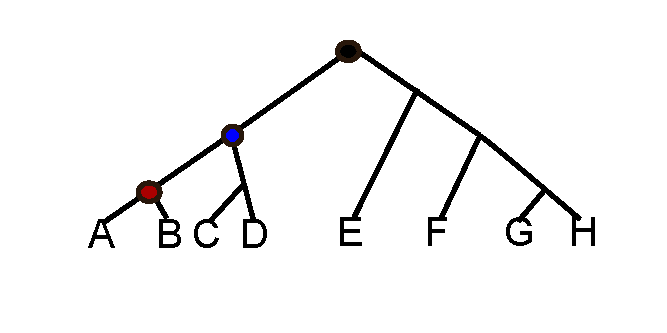
\includegraphics[scale=0.8]{background/phylogeny.pdf}}
\end{center}
\caption[A rooted phylogenetic tree.]{\label{back:phylo_tree} Example of a rooted phylogenetic tree.}
\end{figure}



\subsection{Alignment estimation}\label{back:alignment}

Start with a simplified view of sequence evolution.  There is a DNA sequence at the root.  It evolves down tree through series of substitutions and indels (Fig.~\ref{back:mutations}).  At the end of the process is are sequences that are homologous; they all descended from a common sequence.  A phylogenetic analyses will typically begin by collecting a set of homologous sequences from a common source, such as gene protein sequence.  This is the end result of the sequence evolution process; the history of the changes is lost.  Due to insertion and deletion events, the sequences are all of different length.  Typically a first step in estimating a phylogeny is to first estimate a \emph{Multiple Sequence Alignment} (MSA).  An MSA is a matrix where each row contains a sequence and each column represents shared homology for all biomolecular characters in that column.  

There are many different methods for estimating MSA, including Bayesian techniques (BAli-Phy) that co-estimate alignments and trees, progressive alignment techniques that use a guide tree to pairwise align the sequences (ClustalW, T-COFFEE), iterative methods that use a guide tree, but iterate to obtain better guide trees (Muscle, Mafft, SATe).  

\textbf{NAM:Add more formal definition, citations}.

\subsection{Phylogeny estimation}\label{back:phylogeny}

Once an alignment has been estimated, a phylogeny can be estimated based on various methods such as Maximum Parisomony (TNT and PAUP*), distance-based methods (NJ, UPGMA, FastME), Maximum Likelihood (RAxML, FastTree), or Bayesian methods (Mr. Bayes).  

\textbf{NAM:Add more formal definition, citations}.

\section{Hidden Markov Models}\label{back:hmm}

\textbf{Add text discussing problems of using a single HMM to represent divergent sequences, motivate the HMM families in the next chapter}
\begin{figure}[htbp]
\centering
{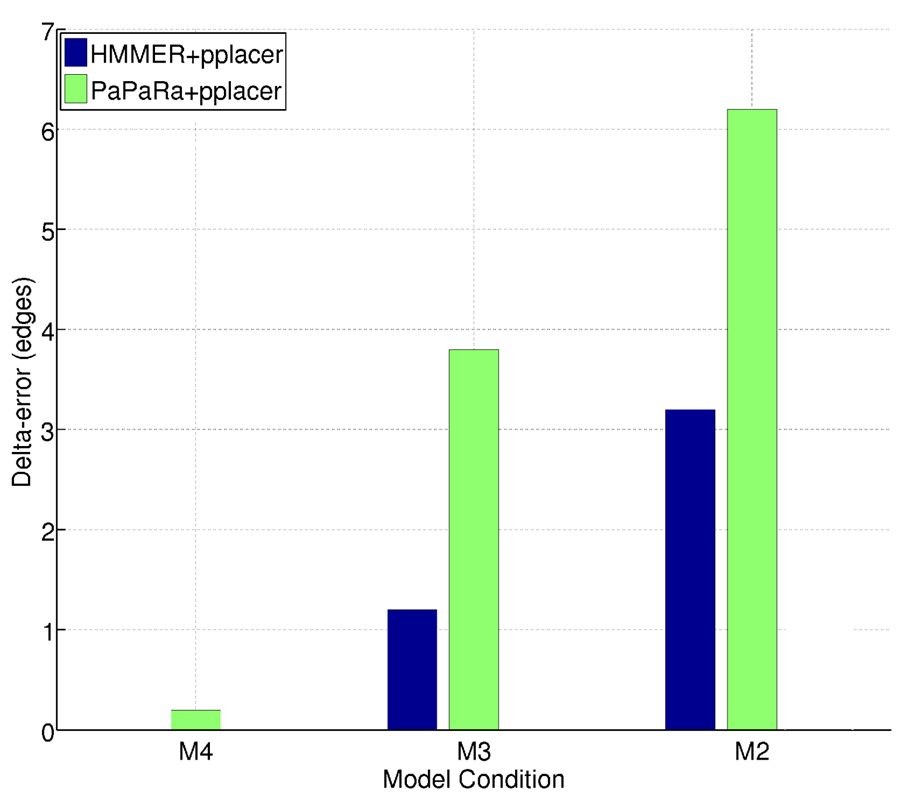
\includegraphics[width=0.80\textwidth]{sepp/hmmer_papara}}
\caption[Comparison of HMMALIGN+pplacer and PaPaRa+pplacer.]{Comparison of HMMALIGN+pplacer and PaPaRa+pplacer under 3 different model conditions, ranked in order of increasing rate of evolution.  Thus, M4 is the slowest evolving dataset, and M2 is the fastest evolving dataset.  The number of sequences in the backbone set is 500 for all model conditions.} 
\label{background:initial}
\end{figure}


\textbf{NAM:Add more formal definition, citations}.
\section{Metagenomic analyses}\label{back:metagenomic}

\textbf{NAM:Add more formal definition, citations}.
\subsection{Taxonomic identification}\label{back:taxonomic_id}

\textbf{NAM:Add more formal definition, citations}.
\subsection{Taxonomic profiling}\label{back:taxonomic_profiling}

\textbf{NAM:Add more formal definition, citations}

\chapter{Families of Hidden Markov Models}
\index{Families of Hidden Markov Models@\emph{Families of Hidden Markov Models}}\label{hmmfamily}

One basic technique for aligning a sequence to an existing backbone alignment is to build a HMM on the backbone alignment, and then align the sequence to the HMM.  In Section~\ref{hmmfamily:motivation}, I present a case study that highlights the weakness of this method on evolutionarily divergent sequences.  Section~\ref{hmmfamily:algorithm}, I present a new technique called \emph{families of HMMs} that allows accurate alignment of divergent sequences.  In Section~\ref{hmmfamily:modification}, I describe modifications of the algorithms.  

\section{Motivation}\label{hmmfamily:motivation}
There exists many databases containing structurally-based alignments that have been manually curated~\cite{Cannone2002,Thompson1999,Punta2012}.  One advantage of using a manually curated alignment is that manual curation can preserve conserved structures that may not be preserved by typically alignment methods.  However, because manual curation requires a large investment of time, the curated alignments often contain small number of sequences.  Thus, one technique for generating a larger alignment from a manually curated alignment is to use the curated alignment as a backbone alignment, and the remaining sequences are aligned to the backbone alignment.  

An example of this approach is within Pfam~\cite{Punta2012}.  Each protein family consists of a seed alignment, a manually-curated alignment.  A HMM is computed on the seed alignment, and the remaining sequences in the protein family are aligned to the HMM to obtain an alignment on the entire protein family.  Often times, the protein family can span from a very diverse range of species.  Thus, the HMM may have difficulty representing an alignment from very evolutionarily divergent species.

In order to explore this issue, I examined an application of the HMM alignment approach under the context of \emph{phylogenetic placement}.  The ``phylogenetic placement" problem is formally stated as follows:

\noindent{\em Phylogenetic Placement Problem. }
\begin{itemize}
\item Input: the {\em backbone} tree $T$ and alignment $A$ on set $S$ of full-length sequences,
and query sequence $s$.
\item Output: tree $T'$ containing $s$ obtained by adding $s$ as a leaf to
$T$.
\end{itemize}

The evolutionary relationship between the query sequence and the full-length sequences can be inferred from the placement location of the query sequence in the tree.

Methods for the first step 
include HMMALIGN\cite{Eddy1998}
and PaPaRa\cite{Berger2011a} method.  
Methods for the second step include 
 EPA\cite{Berger2011} and pplacer\cite{Matsen2010}, which
seek to optimize maximum likelihood
(pplacer also provides a Bayesian approach).
Methods for phylogenetic placement can therefore
be described
by how they handle each step.
Three such methods
include PaPaRa+EPA\cite{Berger2011a},
HMMALIGN+EPA\cite{Berger2011},
and HMMALIGN+pplacer\cite{Matsen2010}.
EPA and pplacer are comparably 
fast and have almost identical 
placement accuracy,
  but have somewhat different memory usage and algorithmic features\cite{Matsen2010};
hence the differences between HMMALIGN+EPA and HMMALIGN+pplacer
do not impact the placement accuracy, and have a minor
impact on running time and memory usage.
The two techniques for computing the extended alignment,
PaPaRa and HMMALIGN, are very different.
HMMALIGN computes a HMM to represent the full-length alignment,
and then aligns each query sequence to that HMM.  In contrast,
PaPaRa uses RAxML to estimate ancestral state 
vectors for each branch in the
tree, aligns the query sequence to every ancestral state
vector, selects the alignment that had the best score and uses
it to extend
alignment $A$ to include $s$.
Consequently, PaPaRa is computationally more 
expensive than HMMALIGN\cite{Berger2011a}, but EPA placements
of query sequences based upon PaPaRa extended alignments can be
more accurate than EPA placements based upon HMMALIGN extended alignments.
However, the improvement in topological accuracy reported\cite{Berger2011a}  for
PaPaRa+EPA over HMMALIGN+EPA was
relatively small, with PaPaRa+EPA placing
query sequences on average
about one edge closer to the correct
location, out of 799 edges. 
Therefore, PaPaRa+EPA and HMMALIGN+EPA are very close
in terms of placement accuracy, although substantially different
in terms of running time.


We investigated the performance of HMMALIGN+pplacer on datasets simulated under 3 different model conditions
with varying rates of evolution from~\cite{Liu2011}.  Each dataset originally consisted of 1000 full-length sequences.  Each dataset was randomly split in half into a query set and a backbone set, each containing 500 sequences.  For each sequence in the query set, 10 different fragments were simulated from the query sequence by selecting a random substring from the query sequence.  On the backbone set, a backbone alignment and tree were estimated using SAT\'{e}-II~\cite{Liu2011}.  We measured the placement accuracy of each query sequence by computing the \emph{delta error}, which is the difference in the number of missing edges of the backbone tree and the backbone tree after the query sequence is inserted into the backbone tree.  

On each dataset, we ran HMMALIGN+pplacer as follows.  An HMM is computed using HMMBUILD on the backbone alignment.  For each query sequence, the extended alignment of the query sequence is estimated by aligning the query sequence to the HMM using HMMALIGN.  Finally, the query sequence is inserted into backbone tree using pplacer.

Figure~\ref{sepp:initial} shows that under
low rates of evolution, both HMMALIGN+pplacer yield very accurate
placements (less than 0.01 delta error), however, as the datasets undergo higher rates of evolution, the accuracy degrades rapidly.

\begin{figure}[htbp]
\centering
{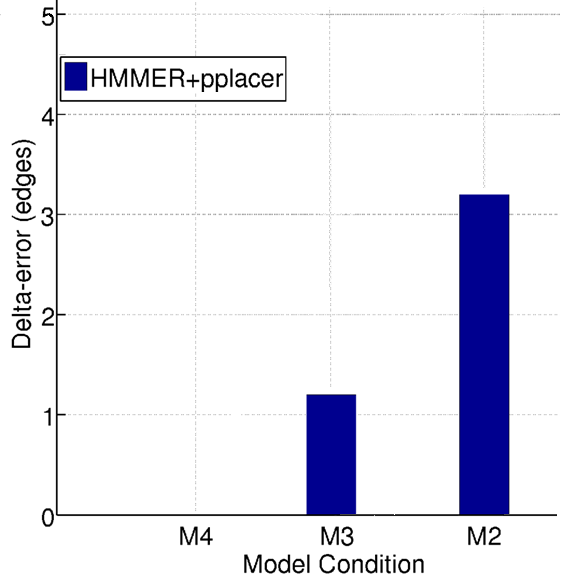
\includegraphics[width=0.60\textwidth]{hmmfamily/hmmer_pplacer}}
\caption[HMMALIGN+pplacer on datasets of varying rates of evolution.]{Comparison of HMMALIGN+pplacer under 3 different model conditions, ranked in order of increasing rate of evolution.  Thus, M4 is the slowest evolving dataset, and M2 is the fastest evolving dataset.  The number of sequences in the backbone set is 500 for all model conditions.} 
\label{sepp:initial}
\end{figure}

In ~\cite{Liu2009}, Liu et al. developed a new alignment and phylogeny co-estimation technique that showed significantly improved alignment and tree reconstruction accuracy on simulated datasets under high rates of evolution (Fig.~\ref{hmmfamily:sate}).  For model conditions simulated under low rates of evolution, all alignment methods had comparable performances.  As the rates of evolution increased, however, alignment and tree accuracy degraded.  This observation lead to the key insight used within \sate: if the evolutionary distance of the sequences could be constrained, then better alignments could be estimated.  By dividing the sequences into subsets of closely related sequences, the evolutionary diameter of the individual subsets is reduced, and more accurate alignments can be estimated on each subset.  The subsets are created using the phylogeny such that sequences that are more closely related will typically fall into the same subset.  This divide-and-conquer approach serves as the basis of the \emph{family of HMM} technique.

\begin{figure}[htbp]
\centering
{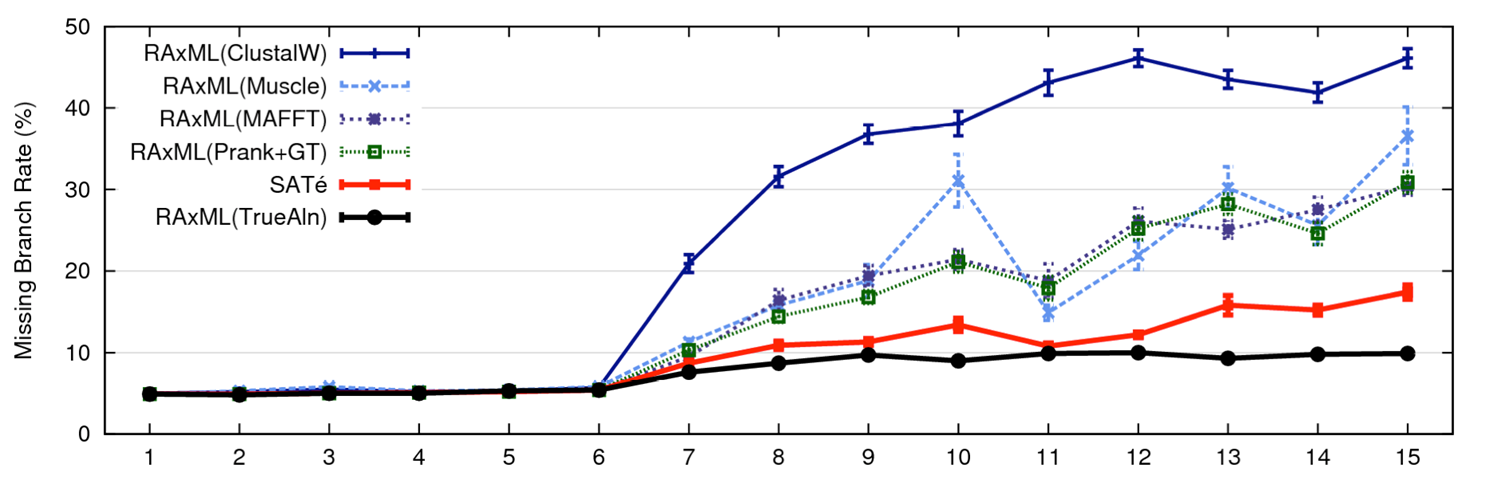
\includegraphics[width=1.00\textwidth]{sepp/sate}}
\caption[Tree error of RAxML trees estimated on different alignment methods.]{Missing branch rate of RAxML trees estimated on different alignment methods under different model conditions (taken from \cite{Liu2009}).  Each model condition was ranked by difficulty; the higher the model condition number, the more evolution has taken place.} 
\label{hmmfamily:sate}
\end{figure}

\section{Families of HMM}\label{hmmfamily:algorithm}
The \emph{families of HMMs} is a technique for aligning a query sequence to a backbone alignment.  The basic outline of the technique is to divide the backbone alignment into subalignments of closely related sequences.  HMMs are computed on each of the subalignments.  We call the HMMs produced by this technique the families of HMMs.  To align a query sequence, we score the query sequence against each HMM, and select the HMM that gives the best alignment score.  We align the query sequence to the HMM, and by transitivity, extend the alignment of the query sequence to the entire backbone alignment.  The creation of the HMM, scoring of the query sequence against the HMMs, and alignment of the query sequence against the HMM use the software suite in HMMER3~\cite{hmmer}.

I now provide the details of each step.

\paragraph{Building the families of HMM.}
We apply the recursive decomposition technique called the 
``centroid edge decomposition'' \cite{Liu2012} 
to build the family of HMMs (see Fig.~\ref{hmmfamily:decomp}).  
From the backbone tree, we select the centroid edge $e$ 
(one whose removal separates the leaf set into 
approximately two equally 
sized subsets).
We remove $e$ (but not its endpoints) from 
the backbone tree  to produce two subtrees.  
This process is recursively repeated on each subtree with
more leaves than a user-defined threshold $t$.  Thus, at the end
of the decomposition, each subtree has $t$ or fewer leaves, and the leaf set of each subtree defines subset.
The backbone alignment restricted to each of these subsets is
called a ``subset alignment".
 For each alignment subset, we run HMMBUILD to produce an HMM, 
 producing a match state for every site that is not completely gapped. 
 
 \begin{figure}[htbp]
\centering
{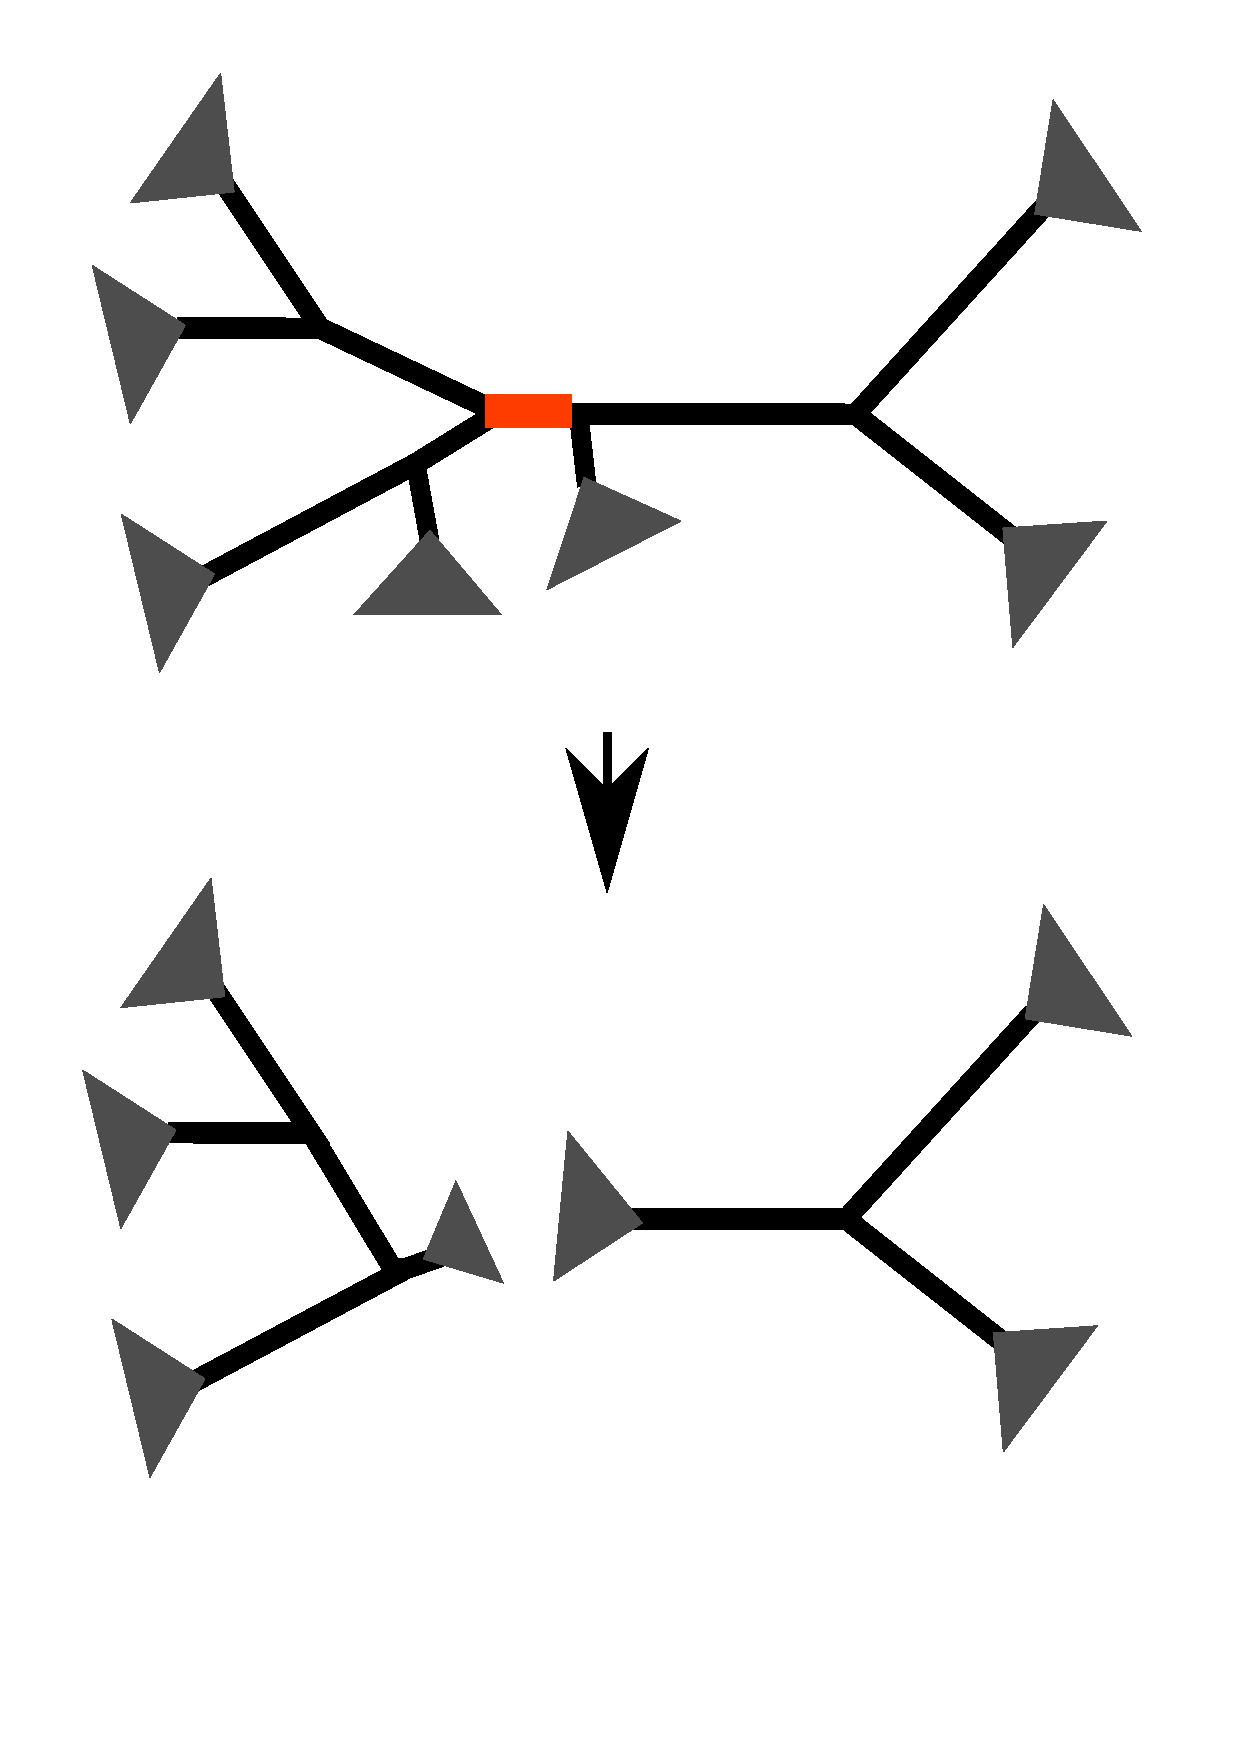
\includegraphics[width=.50\textwidth]{hmmfamily/decomposition}}
\caption[Example of centroid decomposition.]{Example of centroid decomposition.  The centroid edge (colored orange) partitions the tree into roughly two equally sized subtrees.  This edge is removed, and two subtrees are created.  This process is repeated on the subtrees until all subtrees contain at most as many sequences as a user-set threshold.  By default, this is set to 10.} 
\label{hmmfamily:decomp}
\end{figure}


\paragraph{Aligning the query sequences.}
For a given query sequence $q$, it is scored against each of the HMMs using HMMSEARCH, which reports a HMMER ``bit score'', a measure of the quality of the match between the query sequence $q$ and the HMM (see Fig.~\ref{hmmfamily:alignment}).  The HMM that yields the best bit score is selected and an extended subalignment is produced by inserting $q$ into the subalignment using HMMALIGN.  The alignment of $q$ to the entire backbone alignment is computed through transitivity (see Fig.~\ref{hmmfamily:alignment}).

In the special case where a query sequence resulted in no scores against any of the HMMs (i.e., HMMSEARCH reports the sequence as non-homologous to all HMMs), the query sequence is omitted from the final alignment.  

\begin{figure}[htbp]
\centering
{
\includegraphics[width=1.0\textwidth]{hmmfamily/alignment}}
\caption[Example of alignment using HMM families.]{Example of aligning a query sequence using the families of HMMs.  The traditional approach uses a single HMM to align the query sequence.  The families of HMMs uses multiple HMMs.  The query sequence is scored against all HMMs.  The HMM that yields the best score (HMM-1) is selected and the query sequence is aligned to the HMM.} 
\label{hmmfamily:alignment}
\end{figure}

\begin{figure}[htbp]
\centering
{
\includegraphics[width=1.0\textwidth]{hmmfamily/alignment}}
\caption[Example of alignment using HMM families.]{Example of aligning a query sequence using the families of HMMs.  The traditional approach uses a single HMM to align the query sequence.  The families of HMMs uses multiple HMMs.  The query sequence is scored against all HMMs.  The HMM that yields the best score (HMM-1) is selected and the query sequence is aligned to the HMM.} 
\label{hmmfamily:alignment}
\end{figure}


\section{Variations of the algorithm}\label{hmmfamily:modification}



\chapter{SEPP: \sate-enabled phylogenetic placement}\label{sepp_chapter}
\index{SEPP@\emph{SEPP}}%
Metagenomic datasets contain thousands to millions of short
reads, many from different species and for different genes.
Identifying the lineage of the reads is a fundamental step
in metagenomic analysis.  One approach is through phylogenetic
placement.  Under the assumption that all short reads are from
the same gene and that a tree and alignment for a large
number of full-length sequences for that gene are 
available, each short read  can be placed into a phylogenetic
tree, thereby enabling species identification for these reads, 
the inference of evolutionary relationships between
the reads, and potentially also the identification of reads coming
from unknown species.  

Because metagenomic samples can contain millions of sequences and the sequences may come from novel lineages, there is a need for efficient phylogenetic placement algorithms that can handle evolutionarily divergent reads.  I
have developed such a method called \sate-enabled phylogenetic placement (SEPP).  Unlike
HMMALIGN+pplacer which uses a single HMM, SEPP uses multiple HMMs to represent the backbone alignment.  SEPP produces more accurate placements than HMMALIGN+pplacer and PaPaRa+pplacer
on evolutionary divergent datasets and is more computationally efficient, both in 
terms of peak memory usage and running time when placing on very large backbone trees.
I show that SEPP can be parametrized for speed or accuracy, depending on the application.  These results
show the advantages of a family of HMMs for representing a multiple sequence alignment, and form the basis of the remaining methods that I present in my dissertation. 

Section \ref{sepp:motivation} formally describes the phylogenetic placement problem and presents previous work that motivated the development of SEPP.  In Section \ref{sepp:algorithm}, I describe the SEPP algorithm.  In Section \ref{sepp:evaluation}, I describe the simulation study designed to evaluate the performance of SEPP.  Section \ref{sepp:results}, I present the results comparing SEPP with two different techniques for phylogenetic placement, which show that SEPP outperforms the other methods on hard datasets and is significantly faster and more computationally efficient on datasets with large backbone trees.  Finally, in Section \ref{sepp:conclusion}, I present possible ways of improving SEPP, as well as outlining extensions of SEPP toward taxonomic identification and profiling and ultra-large alignment estimation.
 

\section{Motivation and previous studies}\label{sepp:motivation}
\textbf{Move this section to chapter 2, to motivate the HMM families approach?}
% The ``phylogenetic placement" problem is 
% formally stated as follows:
% 
% \noindent{\em Phylogenetic Placement Problem. }
% \begin{itemize}
% \item Input: the {\em backbone} tree $T$ and alignment $A$ on set $S$ of full-length sequences,
% and query sequence $s$.
% \item Output: tree $T'$ containing $s$ obtained by adding $s$ as a leaf to
% $T$.
% \end{itemize}
% 
% Several methods have been developed for this problem using
% the following two steps:
% \begin{itemize}
% \item Step 1: insert $s$ into alignment $A$ to produce the
% {\em extended alignment} $A'$
% \item Step 2: add $s$ into $T$ using $A'$, optimizing some criterion
% \end{itemize}
% Methods for the first step 
% include HMMALIGN\cite{Eddy1998}
% and the recently introduced PaPaRa\cite{Berger2011a} method.  
% Methods for the second step include 
%  EPA\cite{Berger2011} and pplacer\cite{Matsen2010}, which
% seek to optimize maximum likelihood
% (pplacer also provides a Bayesian approach).
% Methods for phylogenetic placement can therefore
% be described
% by how they handle each step.
% Three such methods
% include PaPaRa+EPA\cite{Berger2011a},
% HMMALIGN+EPA\cite{Berger2011},
% and HMMALIGN+pplacer\cite{Matsen2010}.
% EPA and pplacer are comparably 
% fast and have almost identical 
% placement accuracy,
%   but have somewhat
% different memory usage and algorithmic features\cite{Matsen2010};
% hence the differences between HMMALIGN+EPA and HMMALIGN+pplacer
% do not impact the placement accuracy, and have a minor
% impact on running time and memory usage.
% The two techniques for computing the extended alignment,
% PaPaRa and HMMALIGN, are very different.
% HMMALIGN computes a HMM to represent the full-length alignment,
% and then aligns each query sequence to that HMM.  In contrast,
% PaPaRa uses RAxML to estimate ancestral state 
% vectors for each branch in the
% tree, aligns the query sequence to every ancestral state
% vector, selects the alignment that had the best score and uses
% it to extend
% alignment $A$ to include $s$.
% Consequently, PaPaRa is computationally more 
% expensive than HMMALIGN\cite{Berger2011a}, but EPA placements
% of query sequences based upon PaPaRa extended alignments can be
% more accurate than EPA placements based upon HMMALIGN extended alignments.
% However, the improvement in topological accuracy reported\cite{Berger2011a}  for
% PaPaRa+EPA over HMMALIGN+EPA was
% relatively small, with PaPaRa+EPA placing
% query sequences on average
% about one edge closer to the correct
% location, out of 799 edges. 
% Therefore, PaPaRa+EPA and HMMALIGN+EPA are very close
% in terms of placement accuracy, although substantially different
% in terms of running time.
% 
% In order to explore the impact of rates of evolution on phylogenetic
% placement accuracy, I investigated the performance of HMMALIGN+pplacer
% and PaPaRa+pplacer on datasets simulated under 3 different model conditions
% with varying rates of evolution.  Figure~\ref{sepp:initial} shows that under
% low rates of evolution, both HMMALIGN+pplacer and PaPaRa+pplacer yield accurate
% placements, however, as the datasets undergo higher rates of evolution,
% the accuracy greatly degrades, though at a slower rate for HMMALIGN.
% 
% \begin{figure}[htbp]
% \centering
% {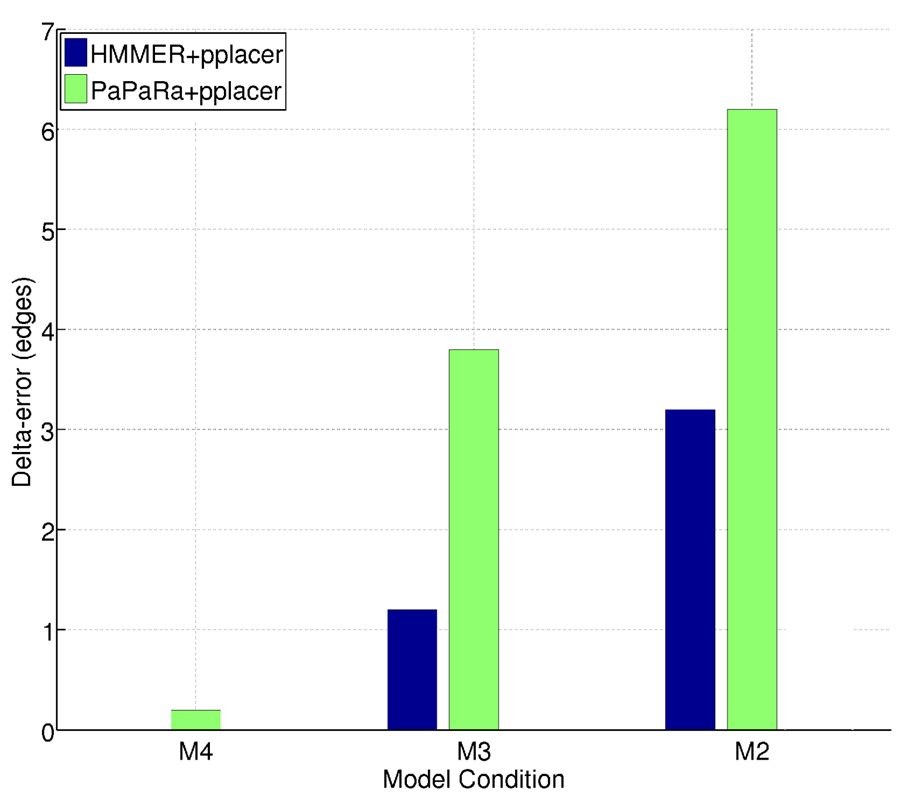
\includegraphics[width=0.80\textwidth]{sepp/hmmer_papara}}
% \caption[Comparison of HMMALIGN+pplacer and PaPaRa+pplacer.]{Comparison of HMMALIGN+pplacer and PaPaRa+pplacer under 3 different model conditions, ranked in order of increasing rate of evolution.  Thus, M4 is the slowest evolving dataset, and M2 is the fastest evolving dataset.  The number of sequences in the backbone set is 500 for all model conditions.} 
% \label{sepp:initial}
% \end{figure}

% In ~\cite{Liu2009}, Liu et al. developed a new alignment and phylogeny co-estimation technique that showed significantly improved alignment and tree reconstruction accuracy on simulated datasets under high rates of evolution (Fig.~\ref{sepp:sate}).  For model conditions simulated under low rates of evolution, all alignment methods had comparable performances.  As the rates of evolution increased, however, alignment and tree accuracy degraded.  This observation lead to the key insight used within \sate: if the evolutionary distance of the sequences could be constrained, then better alignments could be estimated.  By dividing the sequences into subsets of closely related sequences, the evolutionary diameter of the individual subsets is reduced, and more accurate alignments can be estimated on each subset.  The subsets are created using the phylogeny such that sequences that are more closely related will typically fall into the same subset.  This divide-and-conquer approach serves as the basis of the SEPP algorithm.
% 
% \begin{figure}[htbp]
% \centering
% {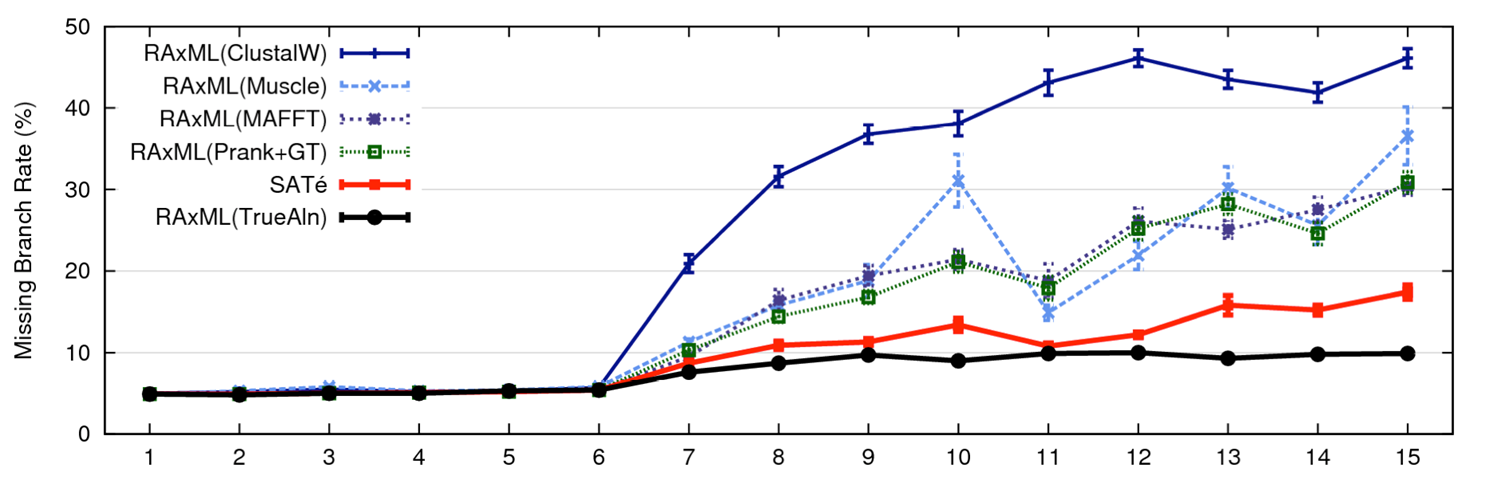
\includegraphics[width=1.00\textwidth]{sepp/sate}}
% \caption[Tree error of RAxML trees estimated on different alignment methods.]{Missing branch rate of RAxML trees estimated on different alignment methods under different model conditions (taken from \cite{Liu2009}).  Each model condition was ranked by difficulty; the higher the model condition number, the more evolution has taken place.} 
% \label{sepp:sate}
% \end{figure}

\section{SEPP algorithm}\label{sepp:algorithm}
SEPP is a meta-method that works with existing
methods for the two steps of phylogenetic placement (computing
the extended alignment, and placing query sequences into
a backbone tree).  SEPP
utilizes upon dataset decomposition technique in
the SAT\'{e}-2 method, which co-estimates sequence alignments and
phylogenies.  This technique takes as input a tree $T$
with leaves labelled by a set $S$ of sequences, a target size $K$,
and it
partitions the set of sequences into smaller subsets, as follows.
SAT\'{e}-2 removes a centroid edge (an edge that
splits the taxon set into two approximately equally sized subsets)
from the input 
tree, thus dividing into two subtrees,
and repeats the process
 until each subset has at most $K$ taxa.
Thus,  the taxa within
any single subset are close together
within the tree and densely sampled within that subset.

The input to SEPP
consists of
\begin{itemize}
\item the backbone tree $T$ and alignment $A$
for the full-length sequences and 
a set of query sequences,
\item
positive integers
\ssa~ and \ssp, with \ssp~$\geq$ \ssa, 
\item a technique for aligning the query sequence
to a multiple sequence alignment of full-length sequences, and
\item
a technique for inserting the query sequence into
a backbone tree, given the extended alignment that
includes the query sequence.
\end{itemize}
The output of SEPP
is the placement of each query sequence into the backbone tree.  The
default methods for SEPP is HMMALIGN for producing the extended alignment
and pplacer for inserting the query sequences into the backbone tree.

%In this study we explore SEPP
%where we use HMMALIGN to produce extended
%alignments and pplacer to insert query sequences into 
%backbone trees.

I now show how SEPP uses the parameters \ssa~ and
\ssp~ to compute the extended alignment and placement of a
set of query sequences
into the tree.
For the sake of simplicity of exposition, I describe this for a single
query sequence.

\begin{itemize}
\item 
SEPP uses the SAT\'{e}-2 decomposition strategy 
to divide the set of taxa in the tree $T$
into disjoint subsets of size at most \ssp.
These subsets are called the ``taxon-insertion-subsets."
\item
SEPP further divides each taxon-insertion subset 
into smaller subsets of size \ssa.
These subsets are the ``alignment--subsets".
Thus, each  alignment-subset is a subset of 
exactly one taxon-insertion-subset.
\item SEPP computes the HMM profile using HMMER for each of the alignment-subsets,
and SEPP finds the alignment-subset that the query sequence $s$ has the best
match to.  HMMALIGN is used to produce an alignment of
$s$ to the backbone alignment on the alignment-subset,
and then that alignment is used to produce the extended alignment for
$S \cup \{s\}$. 
\item 
SEPP finds the taxon-insertion-subset that contains
the selected alignment-subset, and
pplacer is used to insert 
the query sequence $s$ into the 
subtree of the backbone tree induced by the taxon-insertion-subset.
Finally, the location of $s$ in the subtree is used to insert
$s$ into the backbone tree on the entire set of taxa.
\end{itemize}
Thus, the two  parameters \ssa~ and \ssp~ control the
behavior of SEPP.
%We let  \ssa~ range from 10 to 250
%for the simulated datasets and from 10 to 2500 for the biological
%dataset.  We let \ssp~ range from 10 to 500 for the simulated
%datasets and from 100 to 13,822 for the biological dataset.

\section{Performance evaluation}\label{sepp:evaluation}

In order to evaluate SEPP's performance, I compared SEPP 
versus HMMALIGN+pplacer and PaPaRa+pplacer on both 
empirical and simulated datasets.  

I studied performance of these phylogenetic
placement methods on 61 sequence datasets\footnote{All
datasets used in this study are available at 
http://www.cs.utexas.edu/~phylo/datasets.}.
I included 20 simulated 1000-taxon datasets 
that have evolved with substitutions and indels 
from each of three different model
conditions (M2, M3, and M4),
each with the ``medium" gap length distribution
(see Liu et al.\cite{Liu2009} for these data). 
The three model conditions are chosen such
that one dataset is hard, one is moderate, and one is easy.
Because these are simulated datasets,
the true alignment and true tree are known for each datasets. 

I also used
a large bacterial dataset, 16S.B.ALL, with 27,643 16S rRNA sequences, 
originally taken from the Gutell Comparative
Ribosomonal Website (CRW)\cite{Cannone2002}, and also studied by
Liu et al.\cite{Liu2011}.
This dataset has
a curated alignment based upon confirmed secondary (and higher-order)
structures, which are highly reliable.
I use a ML bootstrap tree as the curated
tree for this dataset, retaining only those branches with bootstrap
support above 75\%\cite{Liu2011}. 
Thus, the 16S.B.ALL dataset has a curated tree and alignment as well.

Each dataset was randomly divided into two subsets of equal size,
with one subset ($S$) used to define the backbone alignment and tree,
and the other subset ($R$) used to produce the query sequences.
These query sequences are created by taking substrings of 
normally-distributed lengths (from two distributions, described below), and
with the start positions chosen uniformly at random.

Two categories of reads are generated for each sequence in the M2, M3, and M4
datasets:
``long'' reads, with a mean length of 250 and a standard deviation of 60, 
and ``short'' reads, with a mean length of 100 and a standard deviation of 20.
A total of 10 fragmentary sequences are generated for each sequence,
with half long and half short.  Since
these datasets each include 500 reference and 500 non-reference sequences, 
this process yields 2500 short  and 2500 long reads per dataset.
In summary, each M2, M3, and M4 dataset has a reference tree and alignment 
with 500 taxa and a total of 5000 fragmentary sequences, of which half are
``short" and half are ``long".

For the 16S.B.ALL biological dataset, I create two categories of reads,
with length distributions identical to those of simulated datasets. 
This dataset contains 27,643 taxa, of which I use
13,822 sequences for the backbone tree, leaving me with 13,820 sequences
for creating fragmentary reads. 
For each of these
13,821 sequences, I generated one fragmentary sequence, 
randomly choosing between the long and
short distributions.  Thus, for 
this dataset the backbone tree and alignment has 13,822 taxa, and
there are 13,821 fragmentary sequences.

The sequences in $S$ are used to create two backbone alignments and
trees, as follows.
For sets $S$ that are produced by
simulating sequence evolution,  I have the true alignment and
the true tree.
I restrict each of these (which have 1000 taxa) to the subset of 500
full-length sequences, and then run RAxML
on the resultant tree/alignment pair in order to
optimize the branch lengths and GTR+Gamma parameters.   
This produces the first alignment/tree backbone.
The second backbone alignment/tree pair is produced by running
SAT\'{e} on the set of full-length sequences.
%This analysis produces a tree topology and alignment with 
%GTR+Gamma model parameters optimized
%on this tree/alignment pair.

For the 16S.B.ALL dataset, I use the curated alignment for the
dataset and run RAxML on the alignment to produce a binary
tree.  I then 
restrict the tree to the subset of 13,822 sequences, and 
optimize the branch lengths and GTR+Gamma parameters on the tree
using RAxML.
This produces the first
backbone alignment/tree pair. I use
SAT\'{e} on the subset of 13,822 full-length sequences
to produce the second.
% (with RAxML used to optimize
%the model parameters on the output tree/alignment pair).

I used SAT\'{e} to produce these estimated alignment/tree pairs
because SAT\'{e} produces
more accurate alignments and trees than any two-phase method
(where an alignment is first estimated and then a tree
computed on that alignment)
for these datasets\cite{Liu2011}.
I used SAT\'{e}-2, the new algorithm design for SAT\'{e}, for
these analyses; this produces an alignment and an ML
tree on the alignment estimated using RAxML.
For the 16S.B.ALL dataset, I used FastTree\cite{Price2010}
within SAT\'{e}-2 in each iteration, and finished with
RAxML in order to produce optimized GTR+Gamma parameters on
the final tree.

I classify each query sequence
for its likely difficulty in phylogenetic placement as follows.
I use \hmmer to produce a
HMM profile for the reference alignment, and then to classify the 
query sequences with respect to the HMM profile.
The fragmentary reads are classified as easy to align (``easy") if the obtained
E-value is less than $10^{-5}$, and as ``hard'' otherwise.
Among the hard
reads, there are some reads for which HMMER does not report 
any E-value due to default filtering settings of HMMER. 
I classify such reads as ``very hard" reads.
In earlier phylogenetic placement studies, the hard fragments are
excluded~\cite{Matsen2010}; however,  my study does not 
automatically
eliminate hard fragments.
Many very hard reads are able to be placed by
SEPP, because the reads will receive
E-values with respect to the
smaller alignment subsets.  
Those that fail to be placed at all by SEPP are 
removed from the experimental study; this
process removes 9 from all the
simulated datasets together and 5 from the biological
dataset.

\begin{table}[htbp]
\begin{small} \centering
 \caption{Dataset statistics: 
I present statistics for the true alignments for
the simulated datasets (M2, M3, M4) and
statistics for the curated alignment
on the biological dataset, 16S.B.ALL.
However, a small number of query sequences is
deleted from some of the runs.
}
\begin{center}
\begin{tabular}{clrrllc}
\hline
\hline
Dataset & Type& Size & Num generated     	& Avg 		& Max&  \% gap\\
 	& 	&backbone & query seqs 	& p-dist 	& p-dist & \\\hline
M2 		& sim& 500 & 5000& 0.68 & 0.76 & 67\\\hline
M3 		& sim& 500 & 5000& 0.66 & 0.74 & 53\\\hline
M4 		& sim& 500 & 5000& 0.50 & 0.60 & 51\\\hline
16S.B.ALL 	& emp& 13,822& 13,820 & 0.21 & 0.52 & 74\\
\hline
\end{tabular}
\end{center}
 \label{tab:datasets}\end{small}
\end{table}

Table~\ref{tab:datasets} shows various statistics for the 
true or curated alignment of the datasets included in
our study. The p-distance is the
fraction of sites within an alignment in which two sequences are
different and ``\% gaps" is the percentage of gaps within the alignment.
The empirical statistics show that the datasets vary substantially
in terms of evolutionary distances, with datasets from
model M2 having the largest evolutionary 
distances and 16S.B.ALL having the smallest.

\section{Measurements}
I measure placement accuracy (averaged over
all the query sequences),  running time,
and peak memory usage, for each method on each dataset.
For the simulated datasets I report averages for these
measurements over the 20 replicates in each model
condition.  

% \subsection{Placement accuracy}
% For the most likely
% placement\footnote{Multiple possible placements for
% each read, along with the likelihood of each placement,
% are also provided by pplacer.} of each fragmentary
% read, I first calculate the number of missing branches compared to the 
% reference tree. 
% This number in isolation is hard to interpret, for at least two reasons.
% In the case where \sate~alignment/tree is the input, the backbone tree itself
% contains error. The error of the initial backbone tree is a lower bound on the
% tree error after placement of reads (in fact it is a rather liberal lower bound,
% as the optimal placement of fragments can still have errors higher than the
% initial tree).
% In the case where true or curated alignment/tree is 
% the input, the initial tree has no
% error, but I can still establish useful lower bounds of the tree error. 
% This can be done by using the reference alignment of query sequences 
% to be the backbone alignment as input to the \pplacer. 
% The resulting placement of query sequences
% is the best one can realistically hope for.
% %Siavash - note that randomness is also an explanation for
% %having delta error below 0.  This makes me wonder if we might not just
% %show the delta as the additional error over the error before insertion.
% %ALSO: need to comment on difference between error to true tree and
% %error to ML on true or curated alignment.
% %and perhaps we should show the actual error instead of delta error.

% To account for the lower bounds described above,
% I also define and report 
% the ``delta error" for each technique,  as follows.
% For each read $s$ placed on the \sate~backbone tree, 
% I report the difference between
% the number of missing branches of the initial 
% backbone tree 
% and the number of missing branches after placement of $s$.
% When the backbone tree is 
% the reference (true or curated) tree, 
% I report the
% difference between the number of missing branches of the tree produced by
% placement of $s$ according to the 
% reference alignment of $s$ to $S$ and 
% the number of missing branches
% of the tree after placement of $s$.
% In all cases, 
% the number of missing branches in each tree is defined with
% respect to the reference tree for the taxa in the given tree.
% Thus, the number of missing branches in the backbone trees is
% defined by the reference tree on the set $S$ of backbone taxa, and the
% number of missing branches in the tree produced by placing the
% query sequence into the backbone tree is defined by the
% reference tree on the set $S \cup \{s\}$.


% Note that in the case where the backbone tree is the reference tree, 
% the number of missing branches is
% equal to the node distance between the correct placement of reads and
% actual placements, the error used in the literature\cite{Berger2011,Matsen2010,Berger2011a}. 
% However, this edge distance is not as meaningful as the 
% number of missing branches with respect to either the true or
% curated tree, since estimated trees will generally have error.

\subsection{ Computational aspects}
I report the running times and peak memory usage, each measured
separately for the computation of
extended alignments and placement of query sequences.
These reported values are for 
alignment and placement of all query sequences in each set.
Since some query sequences are deleted from the study as
they cannot be placed, the total number of
query sequences is slightly smaller than the number
generated.
Thus, results for each simulated model condition
are for 99997-100000 query sequences (20 replicas, each with 5000 query sequences),
results for 16S.B.ALL are for 13,819-13,821 query sequences.
Due to memory requirements of PaPaRa and pplacer, 16S.B.ALL experiments are
run on a Linux machine with 16 cores and 256GB of main memory. The results
for simulated datasets are obtained on a heterogeneous condor
cluster.
\section{Results}\label{sepp:results}
\subsection{Algorithm design experiments}

\begin{figure}[htbp]
  \centering
  \subfloat[16S.B.ALL, Curated backbone]
{\label{fig:stt}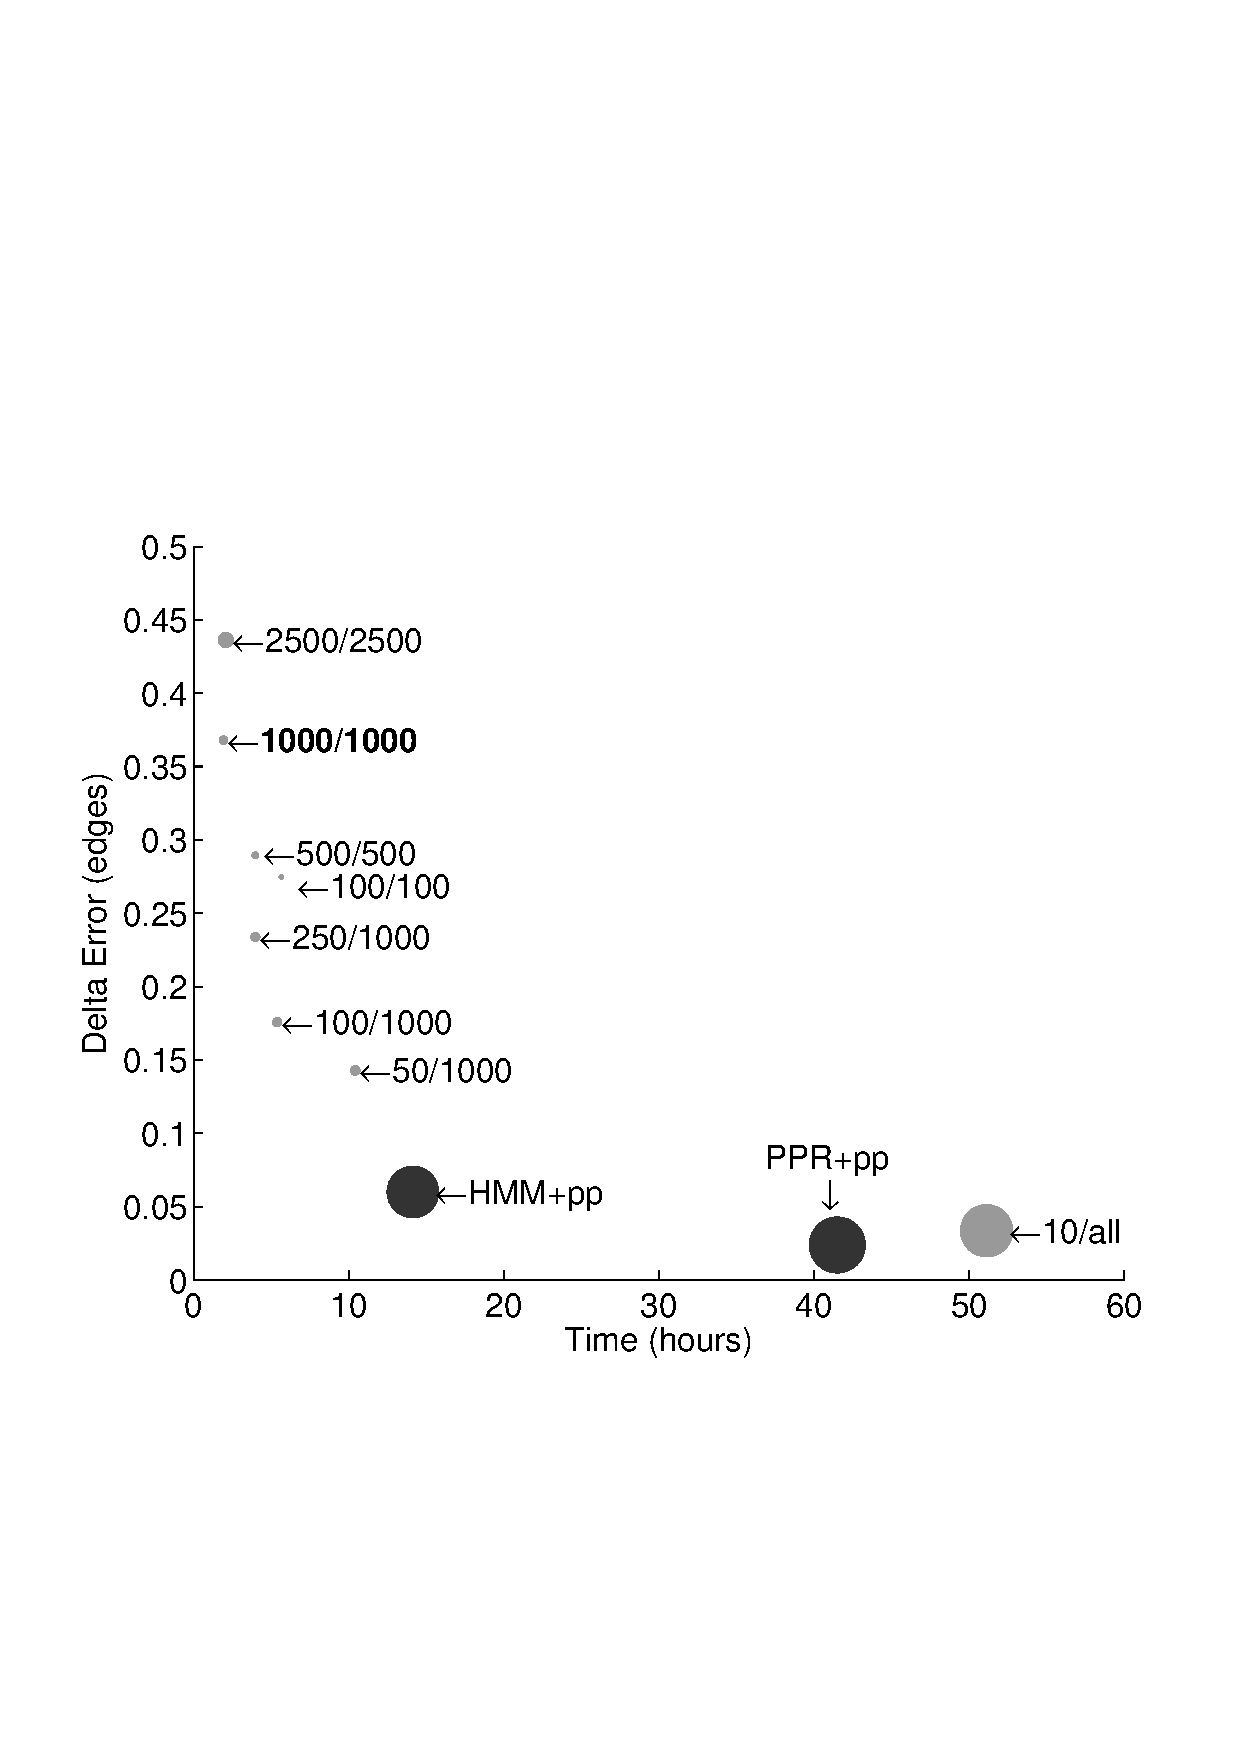
\includegraphics[width=0.70\textwidth]{sepp/scatter-bio-true}}
  \subfloat[16S.B.ALL, \sate~backbone]
{\label{fig:sts}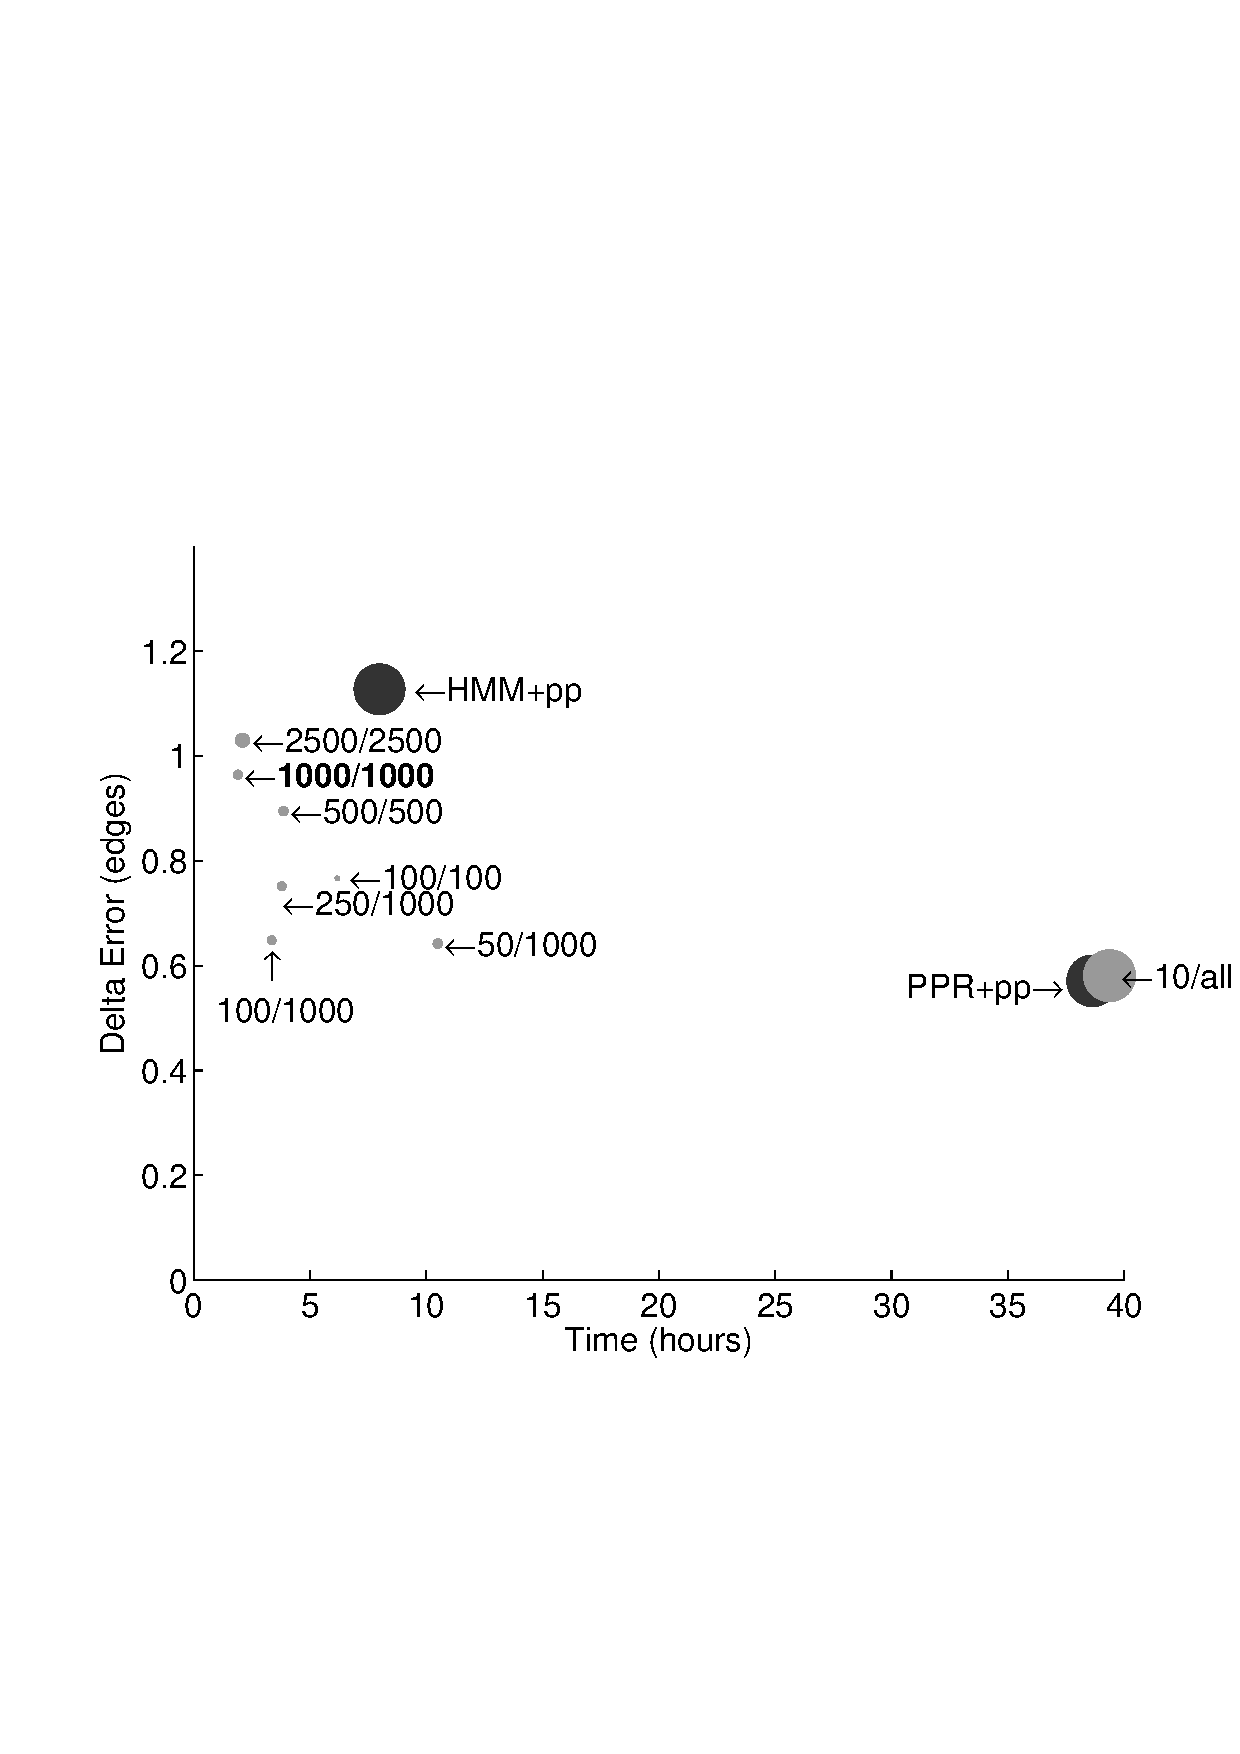
\includegraphics[width=0.70\textwidth]{sepp/scatter-bio-sate}}
\\
  % \subfloat[M2, \sate~backbone]
% {\label{fig:smt}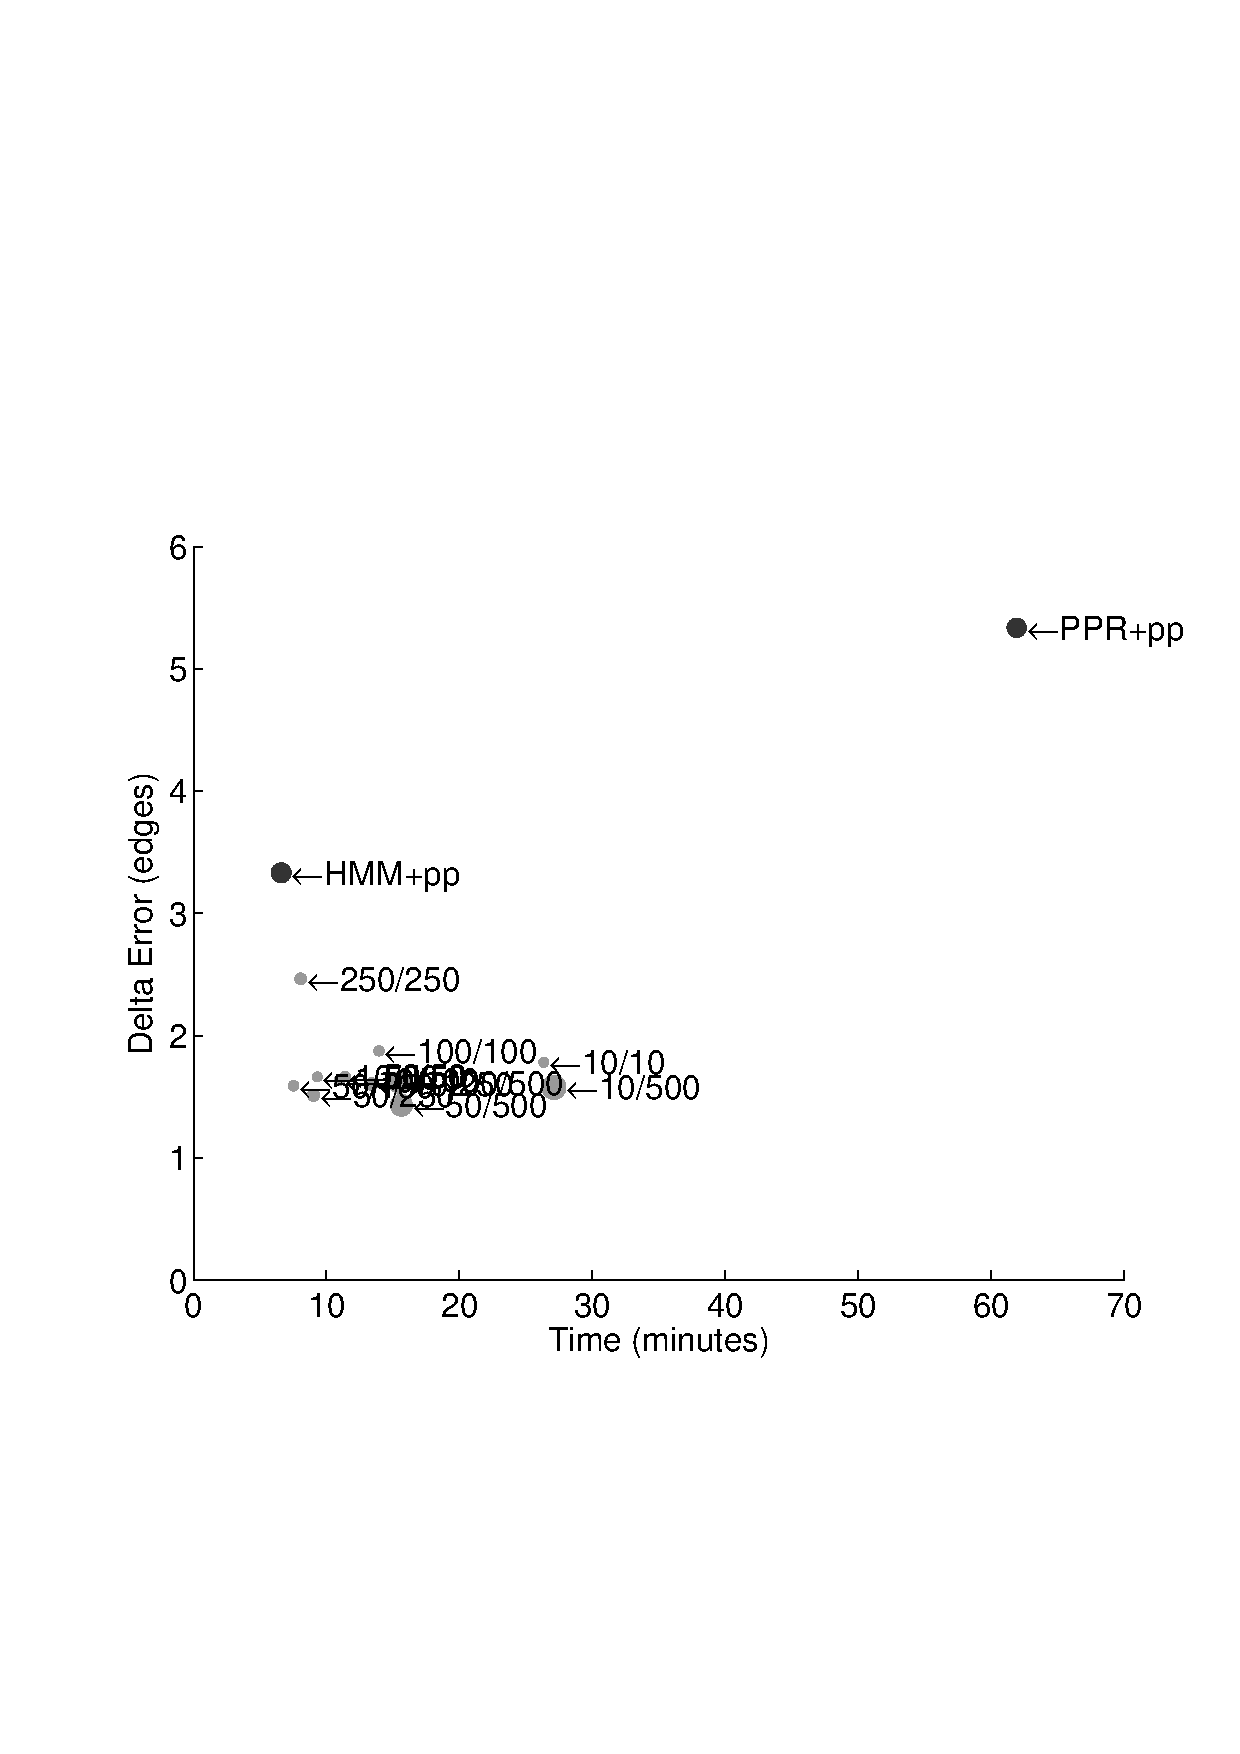
\includegraphics[width=0.5\textwidth]{sepp/scatter-sim-sate}}
  % \subfloat[M2, \sate~backbone - most accurate settings]
% {\label{fig:sms}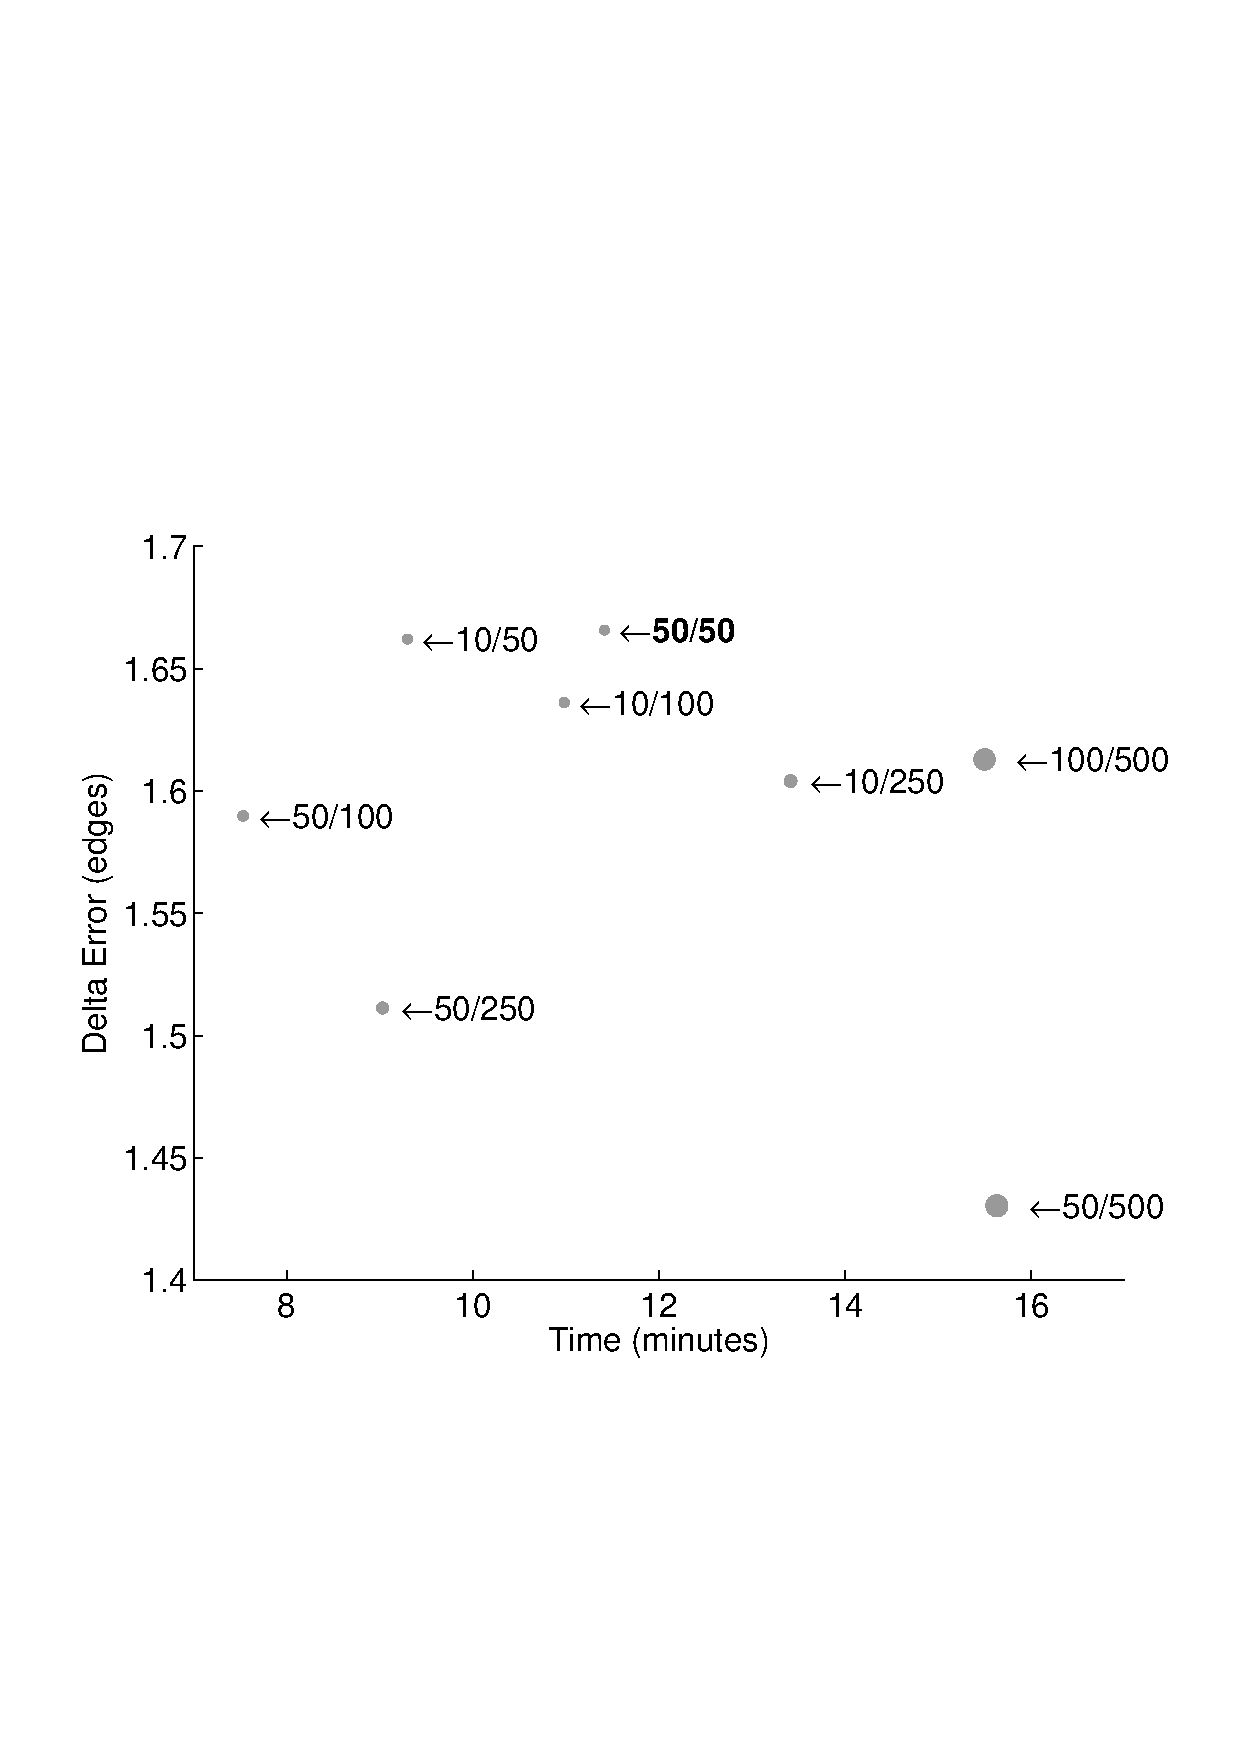
\includegraphics[width=0.5\textwidth]{sepp/scatter-sim-sate-blowup}}
  \caption{Scatter plot of delta error (x) versus time (y) versus memory
(circle diameters). The symbol ``x/y" refers to SEPP(x,y). The default
setting is 1000/1000 for 16S.B.ALL; these points
are bold-faced. Note that the default setting for SEPP is
far from optimal, with other settings providing
better accuracy (and in some cases also better speed).} 
  \label{fig:design-bio}
\end{figure}

\begin{figure}[htbp]
  \centering
  % \subfloat[16S.B.ALL, Curated backbone]
% {\label{fig:stt}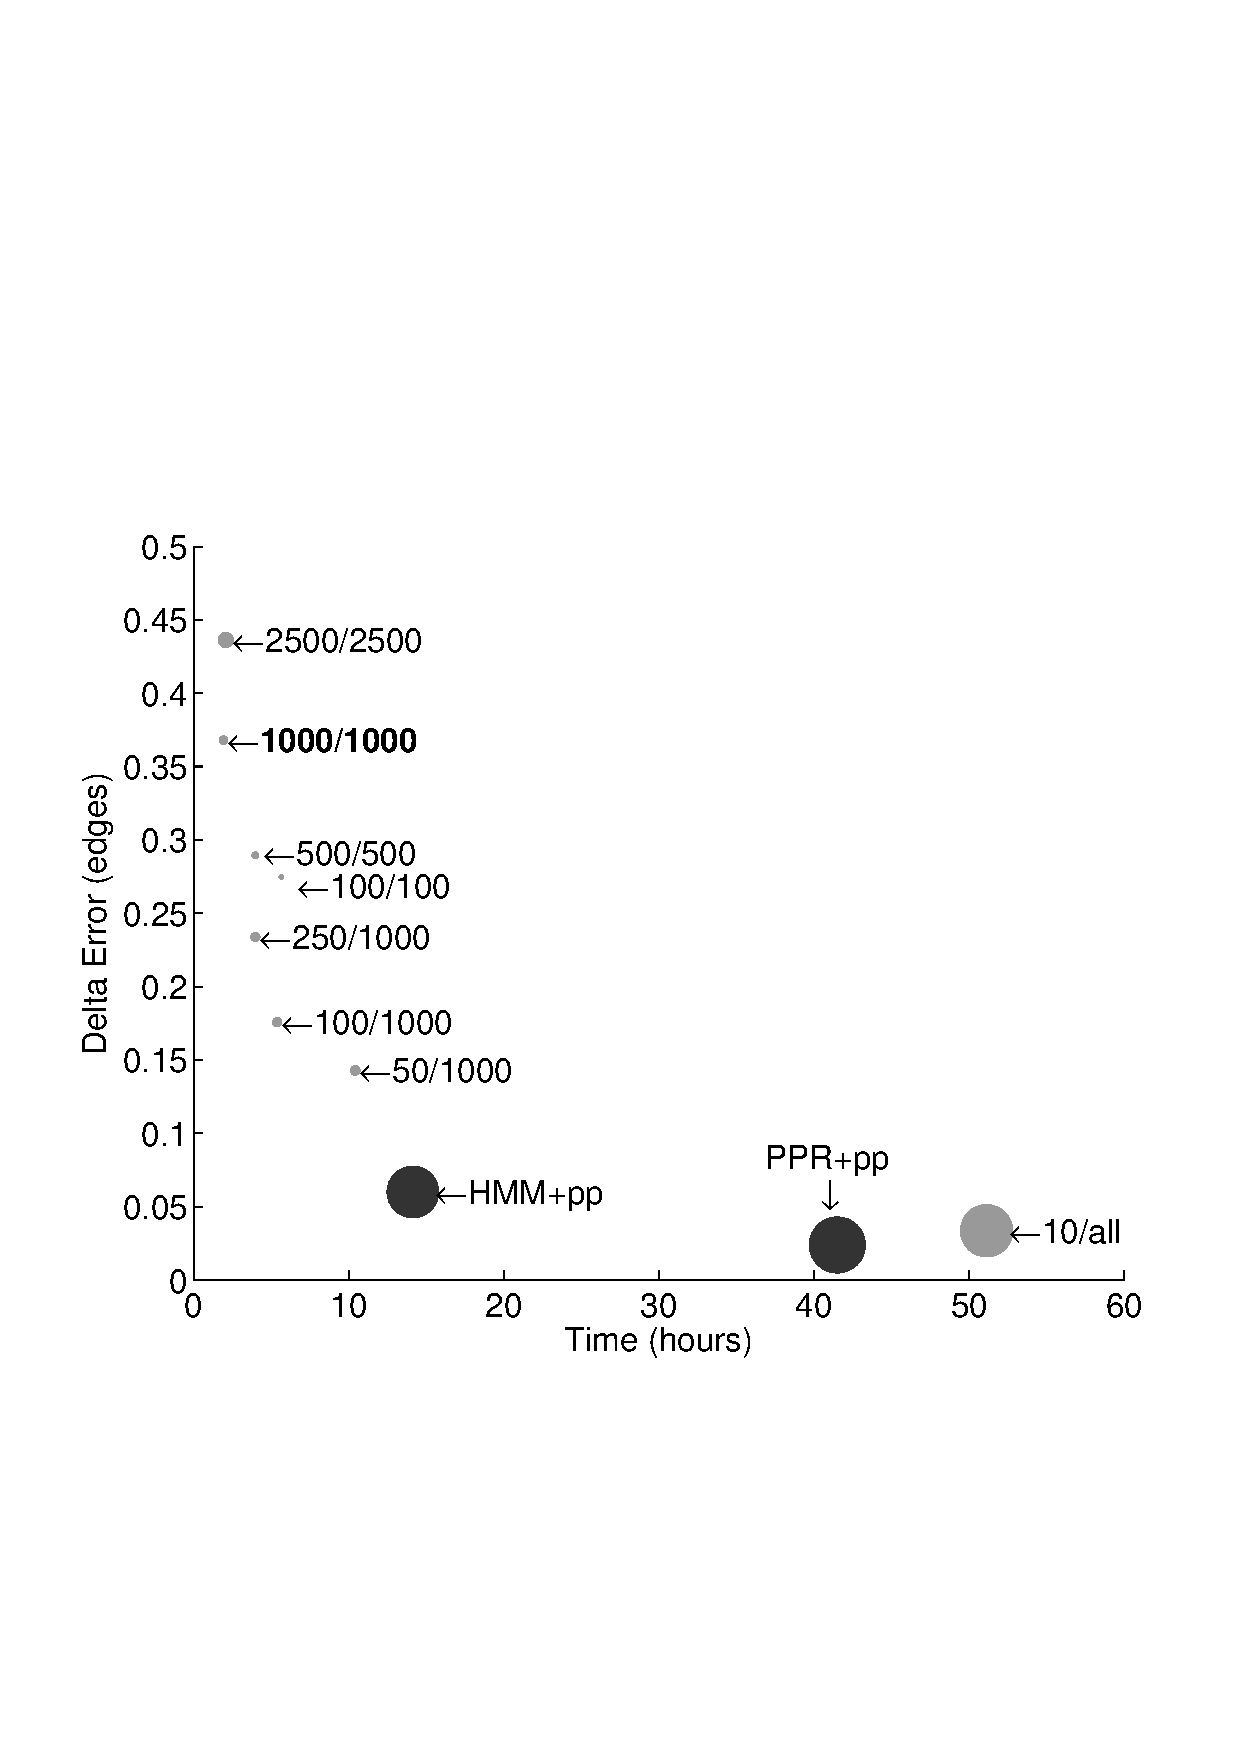
\includegraphics[width=0.5\textwidth]{sepp/scatter-bio-true}}
  % \subfloat[16S.B.ALL, \sate~backbone]
% {\label{fig:sts}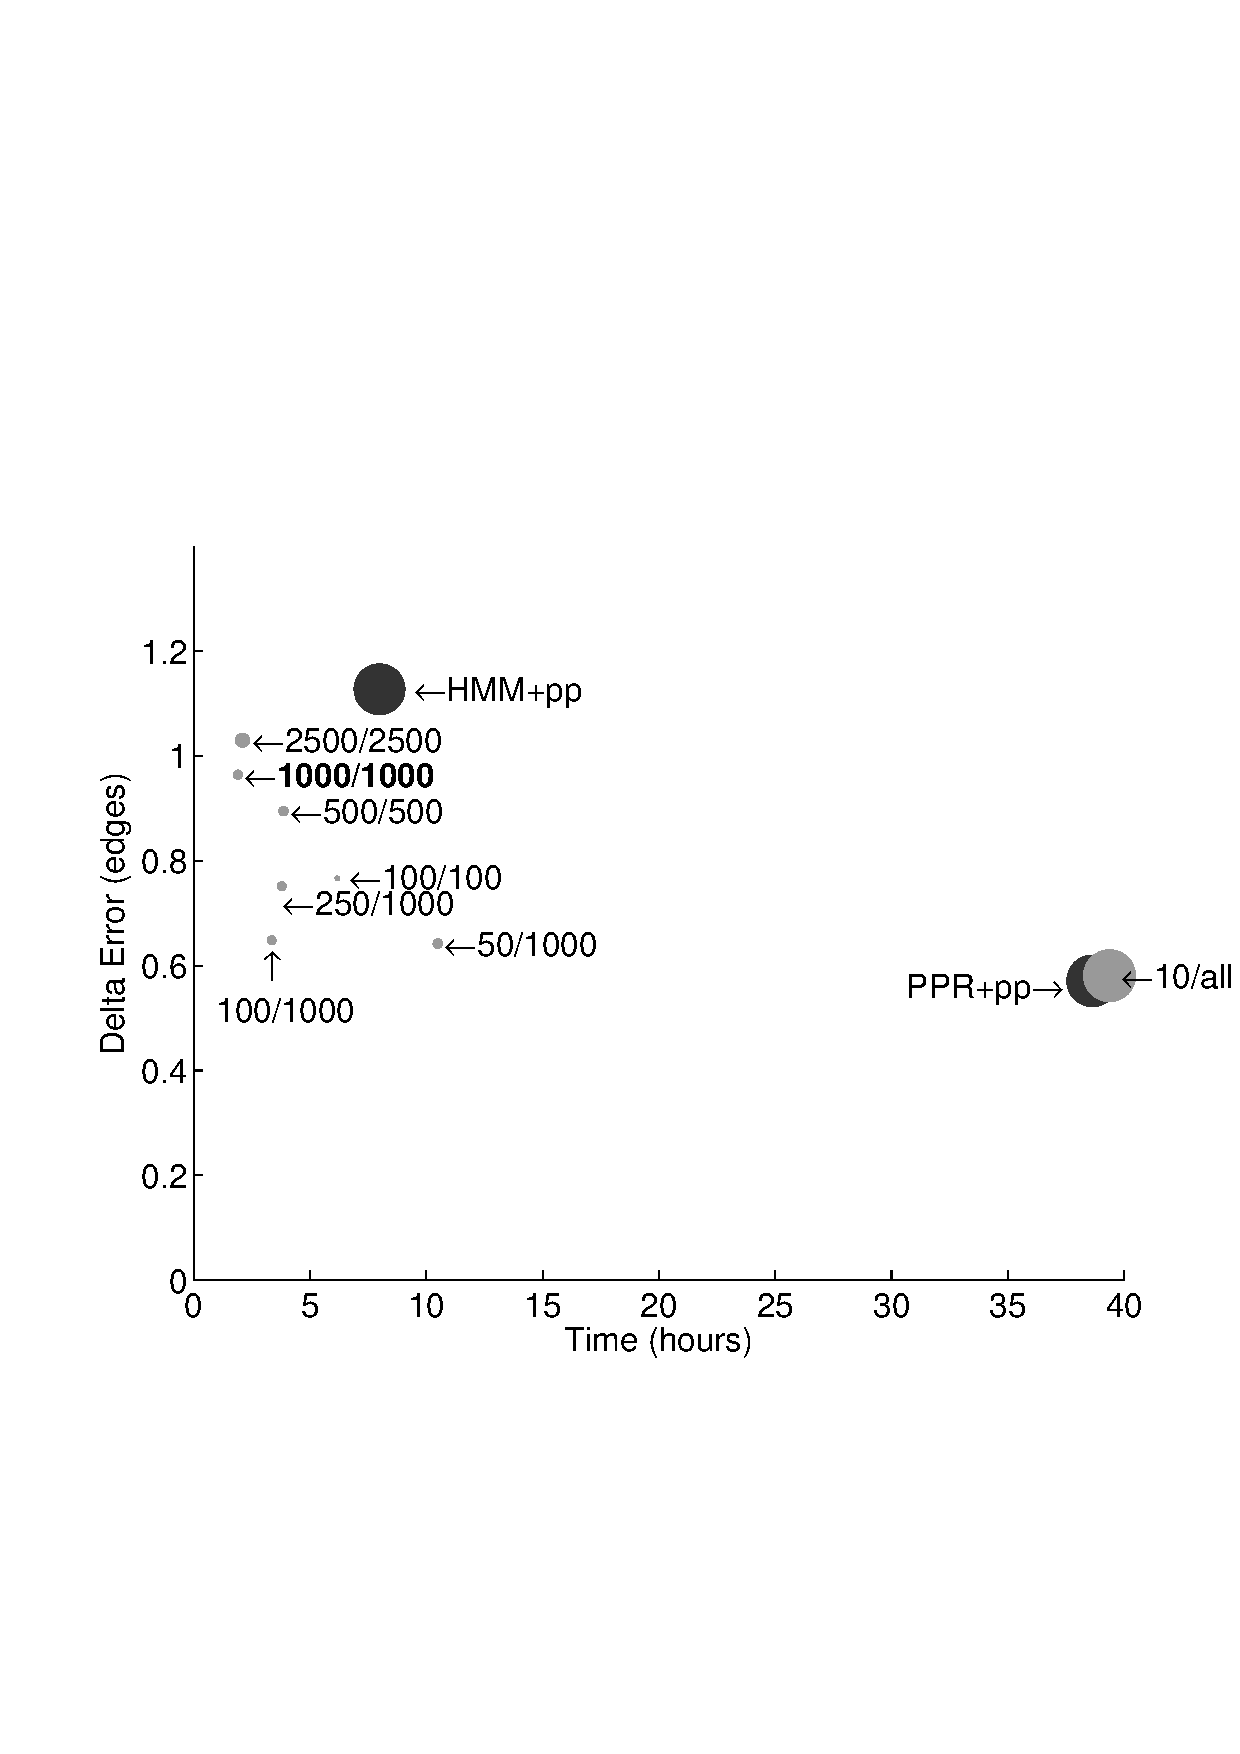
\includegraphics[width=0.5\textwidth]{sepp/scatter-bio-sate}}
% \\
  \subfloat[M2, \sate~backbone]
{\label{fig:smt}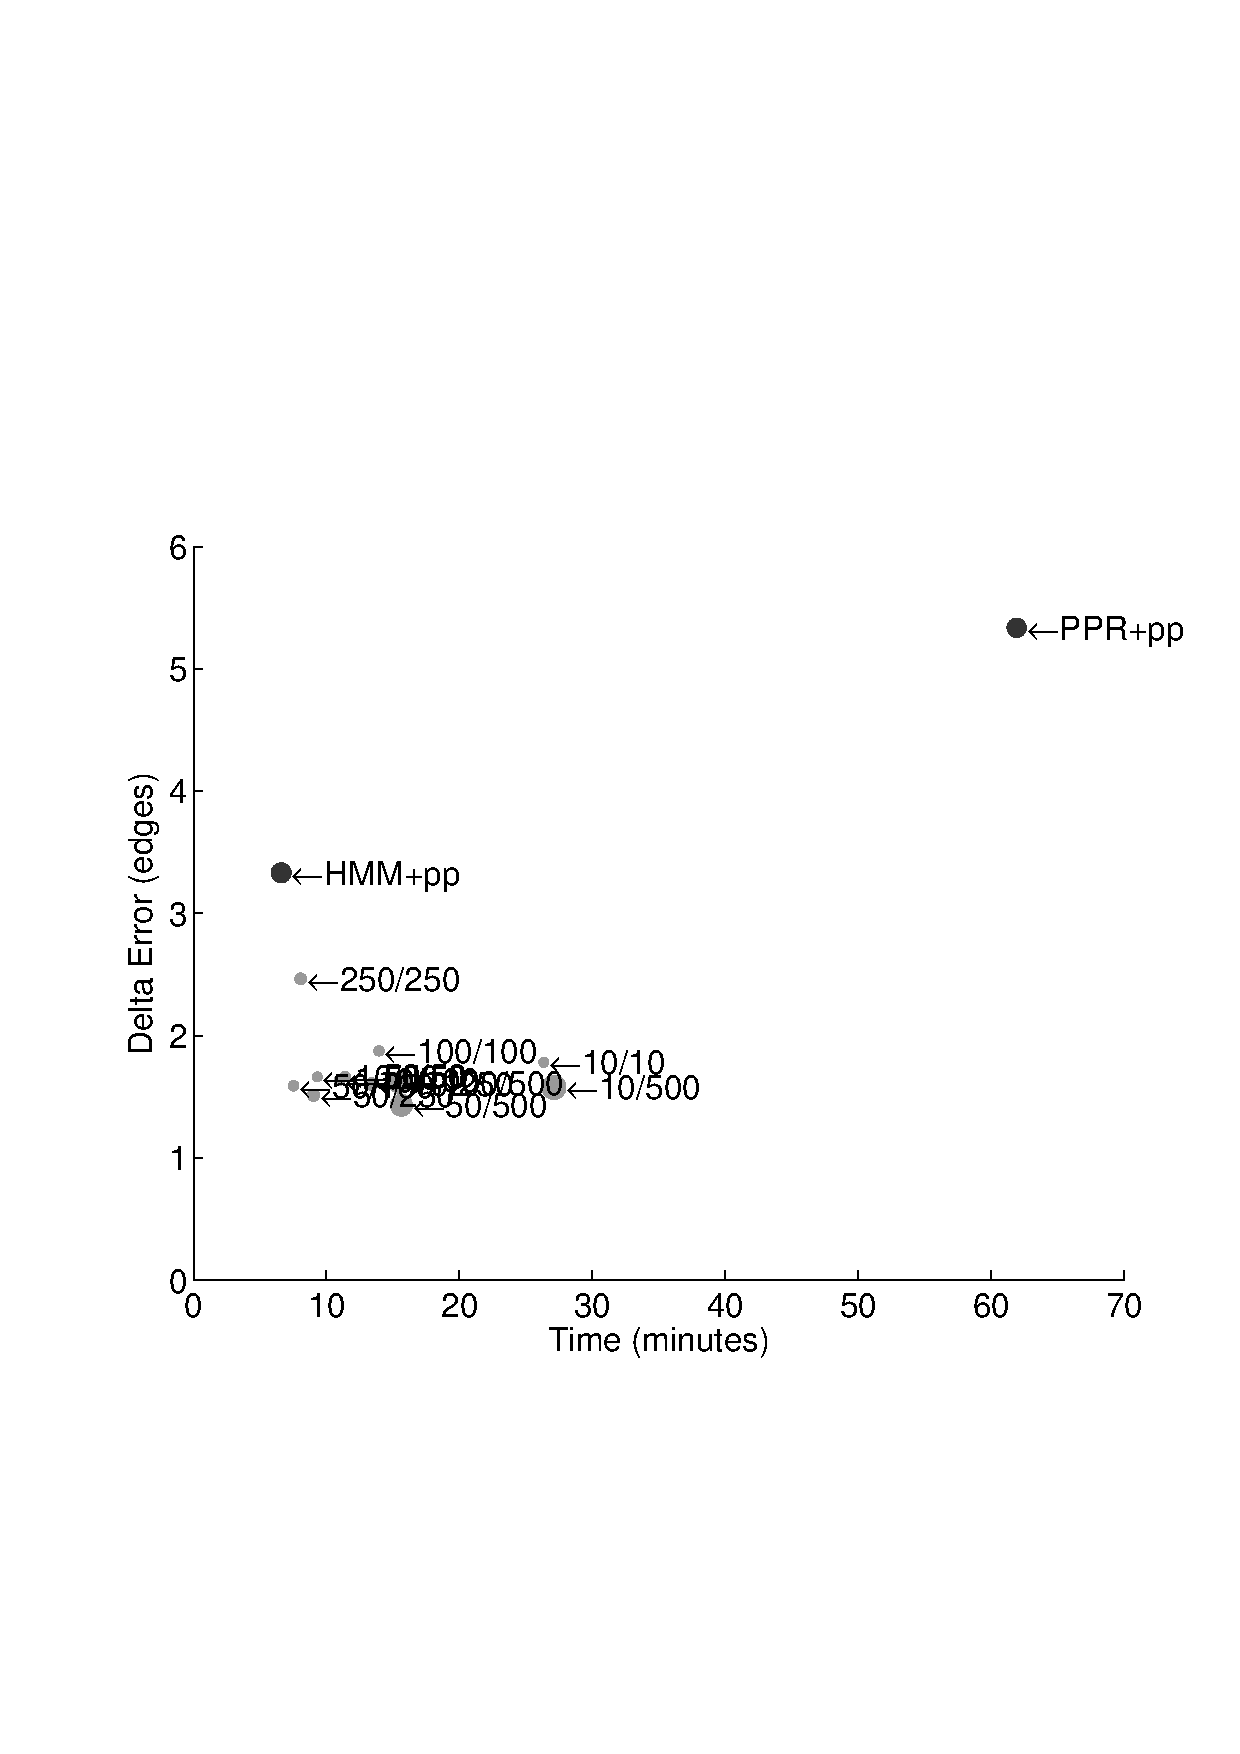
\includegraphics[width=0.70\textwidth]{sepp/scatter-sim-sate}}
  \subfloat[M2, \sate~backbone - most accurate settings]
{\label{fig:sms}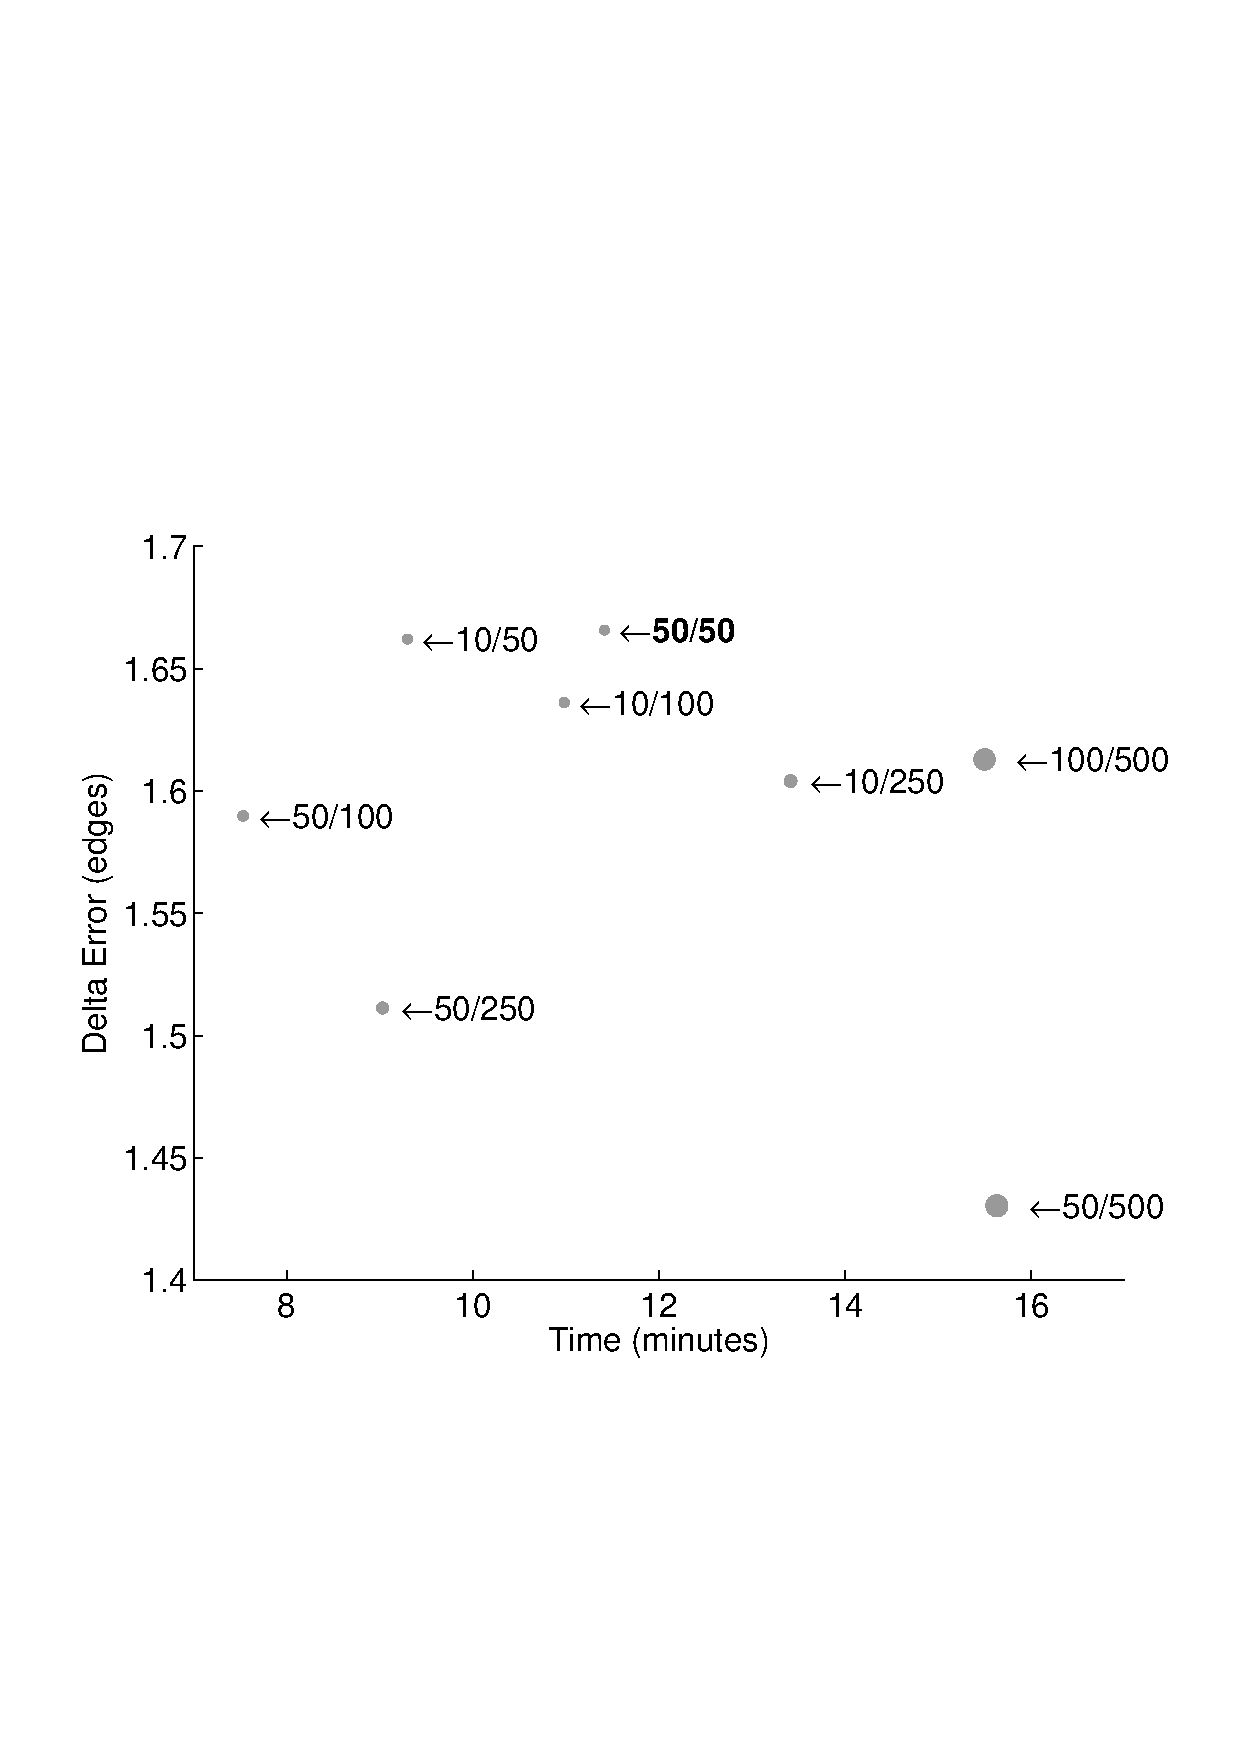
\includegraphics[width=0.70\textwidth]{sepp/scatter-sim-sate-blowup}}
  \caption{Scatter plot of delta error (x) versus time (y) versus memory
(circle diameters). The symbol ``x/y" refers to SEPP(x,y). The default
setting is 50/50 for M2; these points
are bold-faced. Note that the default setting for SEPP is
far from optimal, with other settings providing
better accuracy (and in some cases also better speed).} 
  \label{fig:design-sim}
\end{figure}


Figures \ref{fig:design-bio} and \ref{fig:design-sim} show results 
where I vary the two algorithmic parameters
\ssa~ and \ssp.
Note that decreasing \ssa~ to 50 (and sometimes to 10) 
and increasing \ssp~ tends to
improve the placement accuracy, but at a running time cost.
Also, bigger improvements in accuracy are obtained by decreasing
\ssa~ than by increasing \ssp.  However, for most conditions,
there is a wide range of parameter settings in which the
differences in placement error are quite
small (often less than half an edge), and
within this collection there can be significant differences in running
time.

To set the default parameters, I sought a setting that
worked reasonably well with respect to both
running time and placement accuracy. 
Setting \ssa=\ssp=1000 for the 16S.B.ALL
datasets and \ssa=\ssp=50 for the
simulated datasets  produced good results.  These
settings correspond to setting the subset sizes to about
10\% of the number of taxa in the
backbone tree.
Note, however, that setting \ssa=\ssp=50 is by no means optimal for the M2
model condition (four other settings, with \ssa~at most 50,
have less error and complete faster).
Similarly, setting \ssa=\ssp=1000 is the fastest for the
16S.B.ALL datasets, but more accurate
results can be obtained with other settings (each
with \ssa~below 1000)
for a running time cost.

\vspace{.1in}
\subsection{Comparisons using the default setting for SEPP}

I present results for PaPaRa+pplacer, HMMALIGN+pplacer, and
the default setting for SEPP where we set
\ssa= \ssp~to approximately 
10\% of the number of taxa in the backbone tree. This yields
parameters 50/50 for the simulated datasets (backbone trees have 500
taxa) and 1000/1000 for the 16S.B.ALL dataset (backbone
trees have 13,822 taxa).

\begin{figure}[htbp]
  \centering

%  \subfloat[\sate~backbone]
{\label{fig:sts}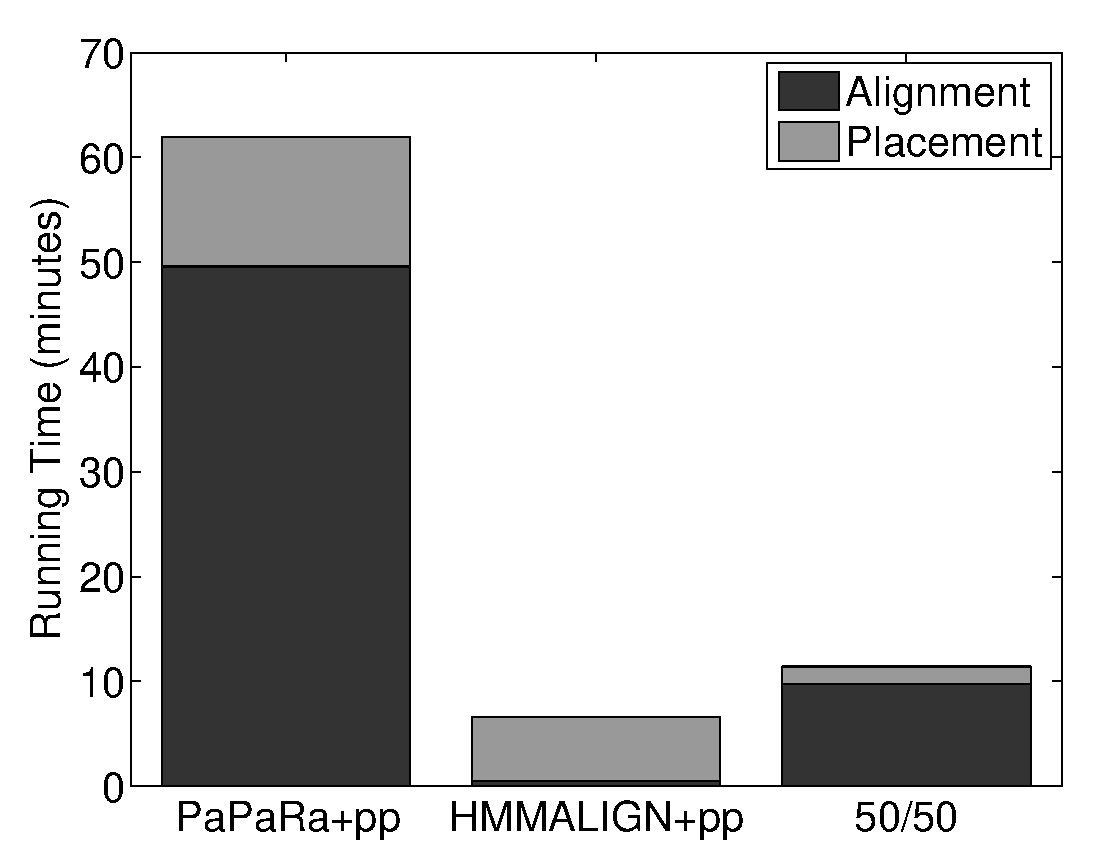
\includegraphics[width=0.35\textwidth]{sepp/M2-time-sate}}
%  \subfloat[True backbone] 
{\label{fig:stt}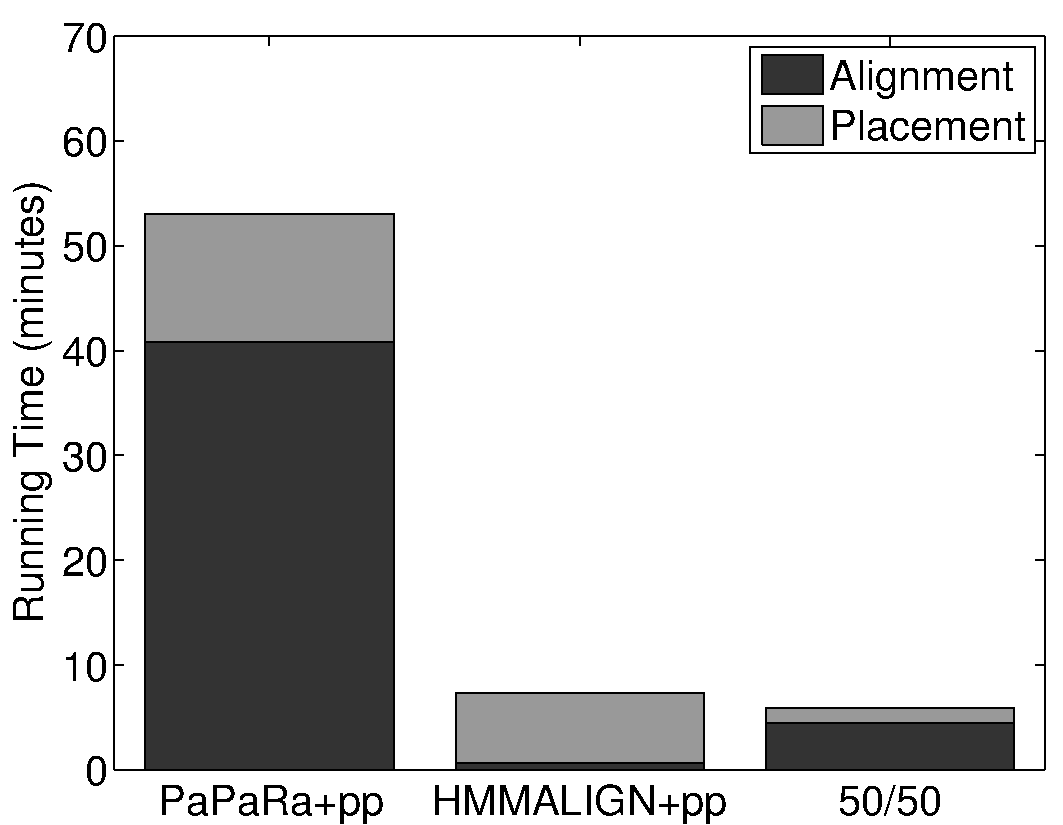
\includegraphics[width=0.35\textwidth]{sepp/M2-time-true}}
\\
%  \subfloat[\sate~backbone]
{\label{fig:sms}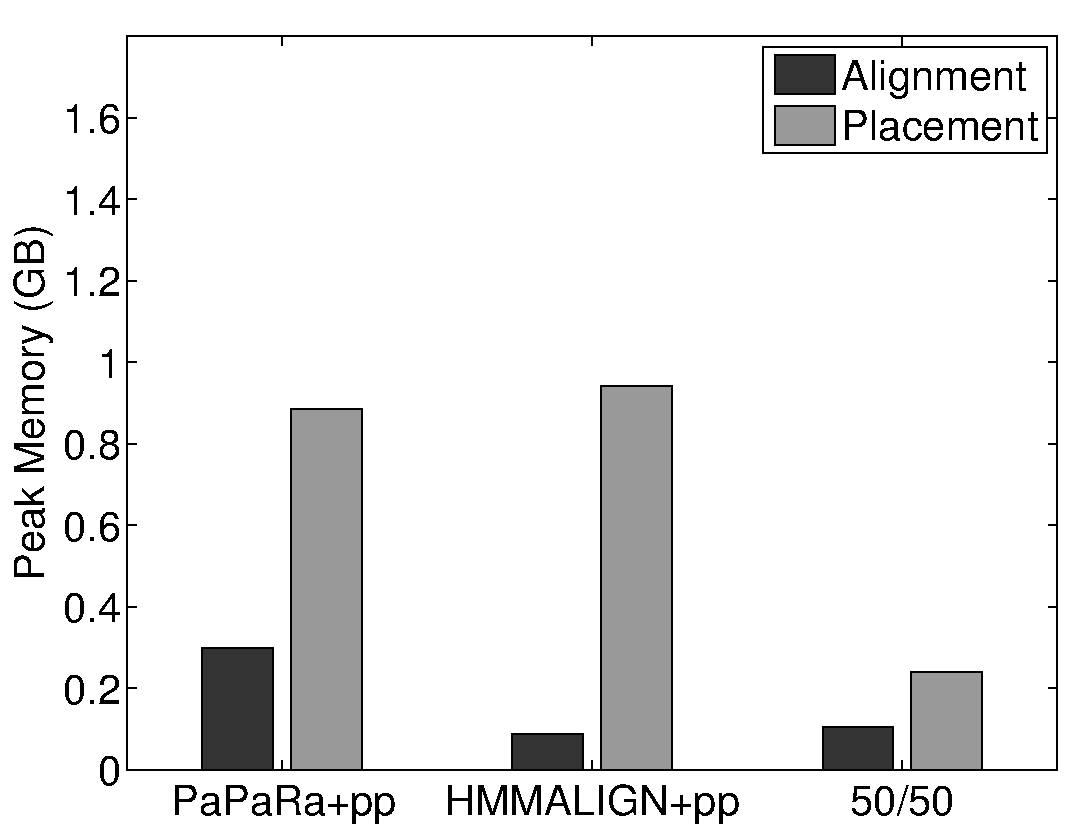
\includegraphics[width=0.35\textwidth]{sepp/M2-mem-sate}}
%  \subfloat[True backbone]
{\label{fig:smt}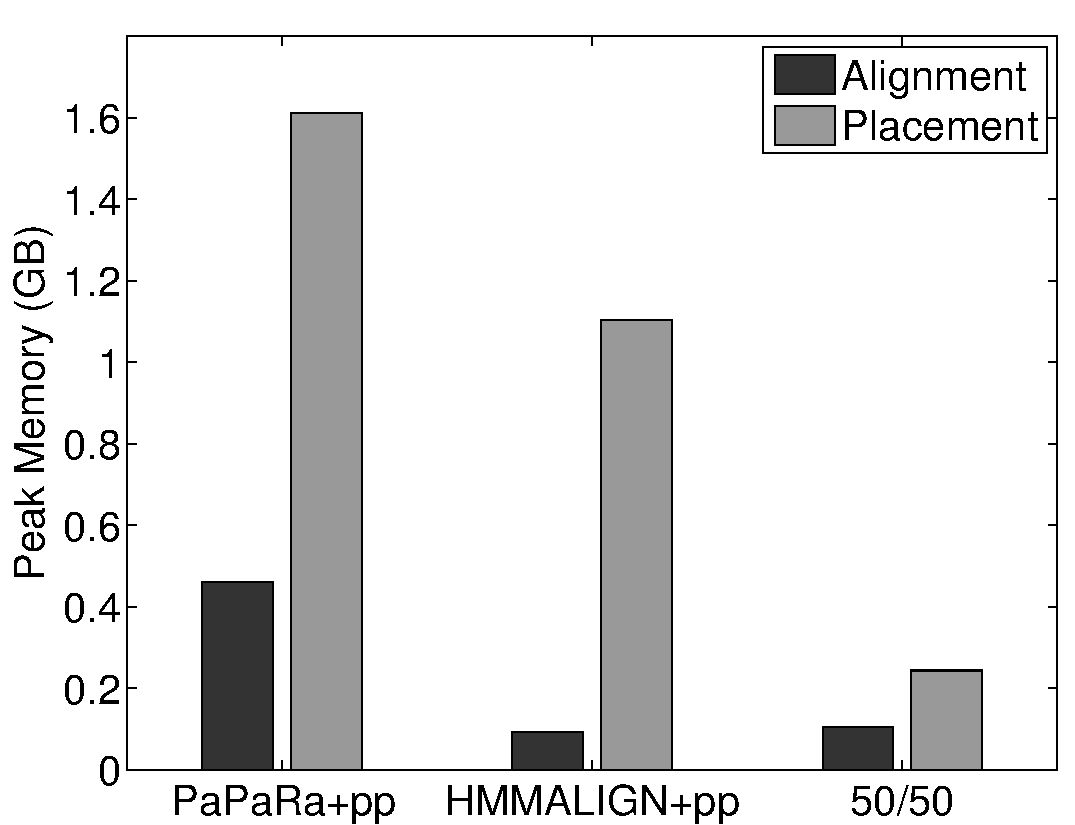
\includegraphics[width=0.35\textwidth]{sepp/M2-mem-true}}
\\
  \subfloat[\sate~backbone]
{\label{fig:ses}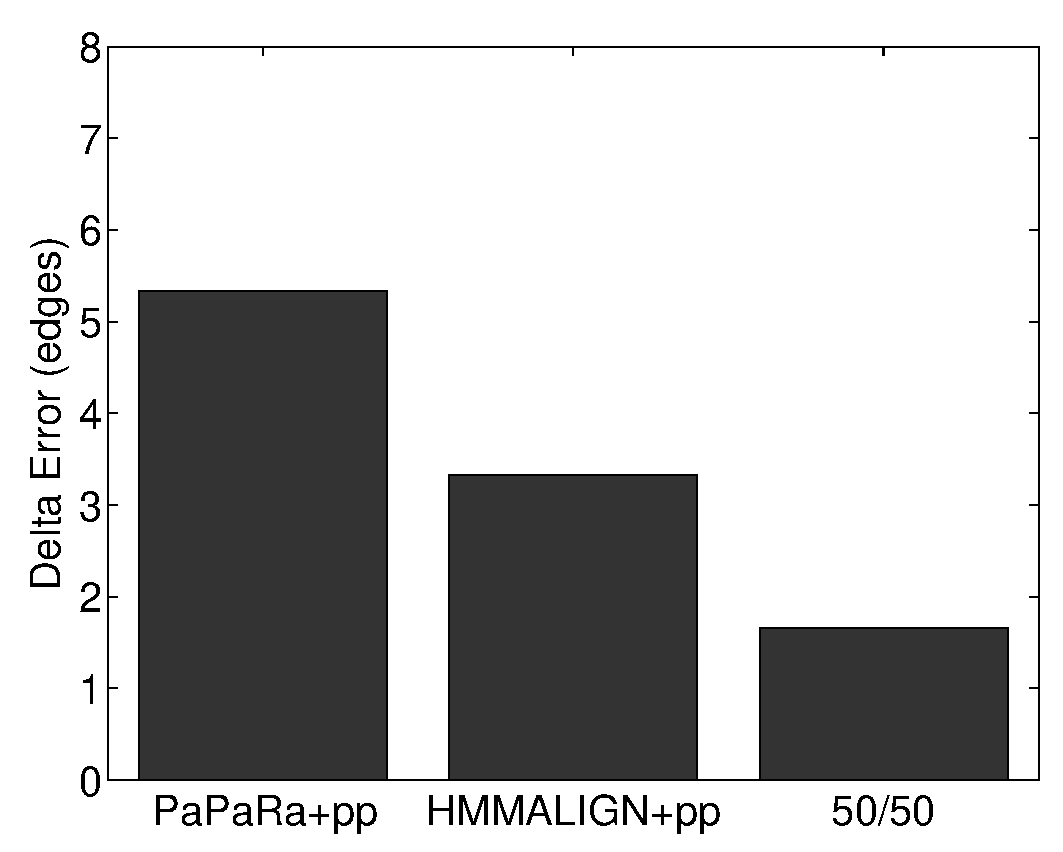
\includegraphics[width=0.35\textwidth]{sepp/M2-err-sate}}
  \subfloat[True backbone]
{\label{fig:set}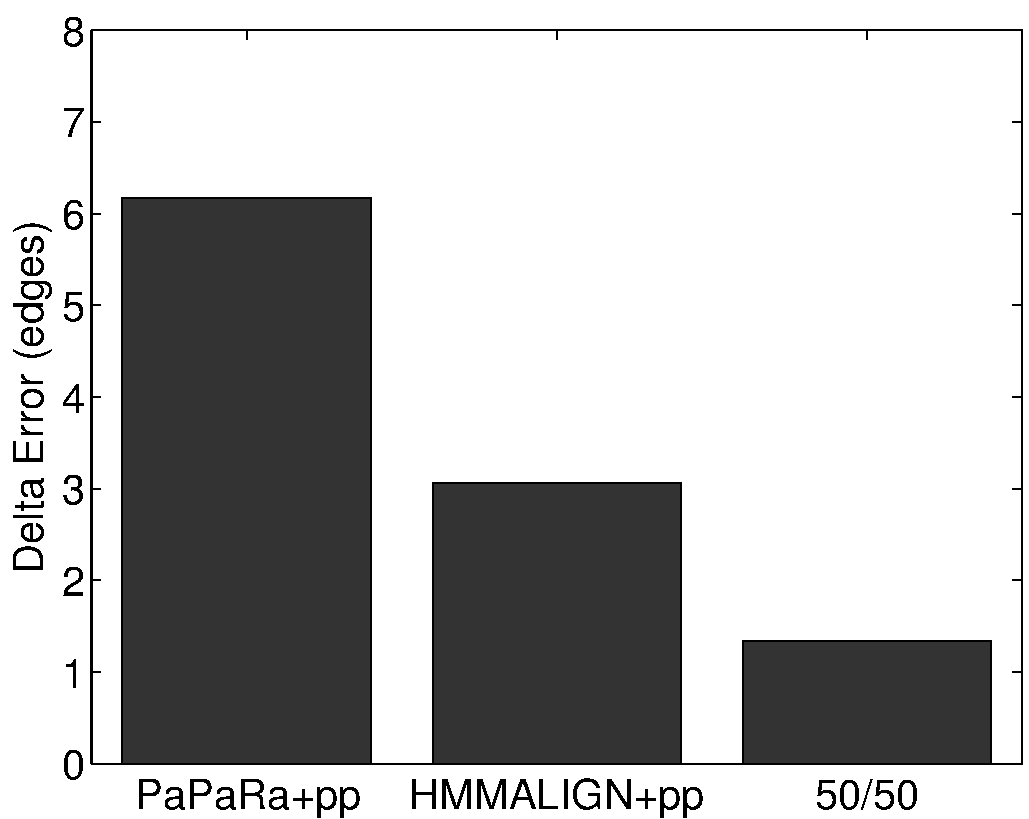
\includegraphics[width=0.35\textwidth]{sepp/M2-err-true}}
  \caption{Results on simulated datasets for model M2. I show running time (top), peak memory
usage (middle), and average number of additional missing branches per
query sequence (bottom).  Results for the SAT\'{e} backbone alignment and tree are on the
left, and results for the true backbone alignment and tree are on the
right.
The SAT\'{e} backbone tree has 12.1\% missing
branch rate and the backbone tree based upon the
true alignment has 0.09\% missing branch rate.
The number of additional missing branches shown (bottom) is the
increment above that amount.
}
  \label{fig:M2}
\end{figure}

\begin{figure}[htbp]
  \centering
%  \subfloat[Running time using \sate~backbone]
{\label{fig:bts}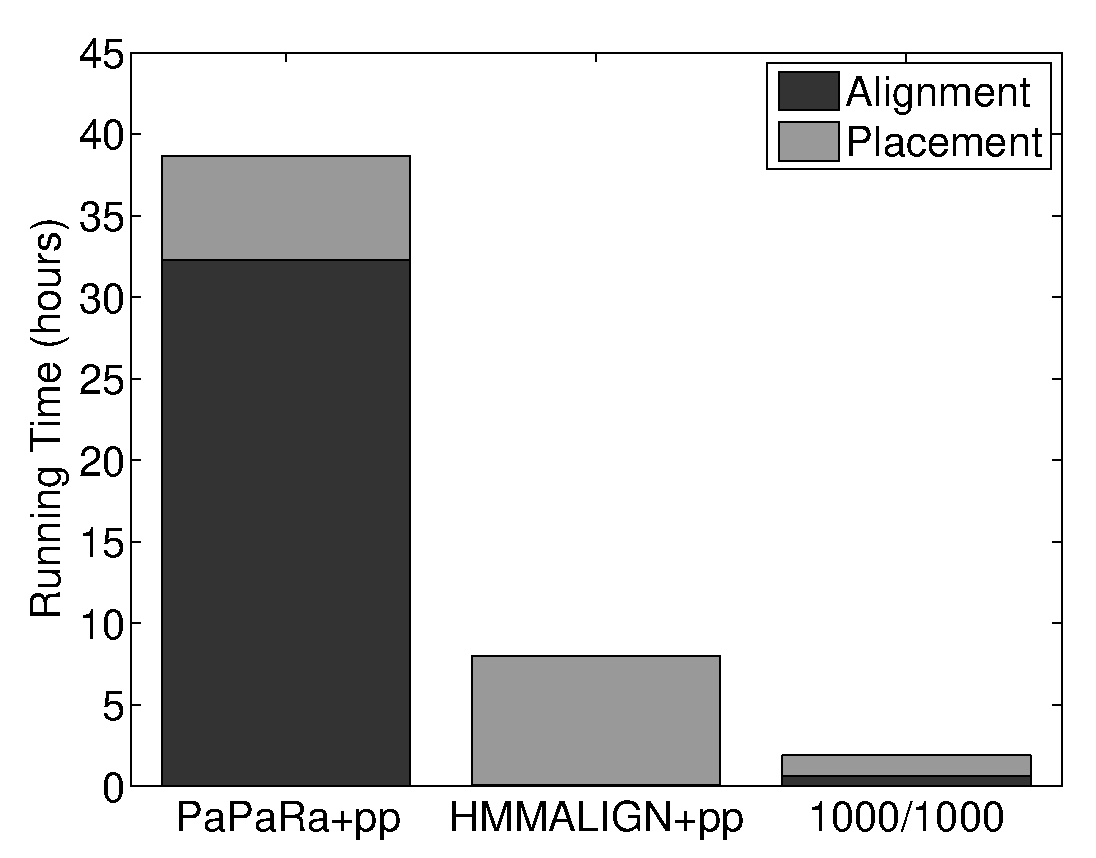
\includegraphics[width=0.35\textwidth]{sepp/bio-time-sate}}
%  \subfloat[Running time using curated backbone]
{\label{fig:btt}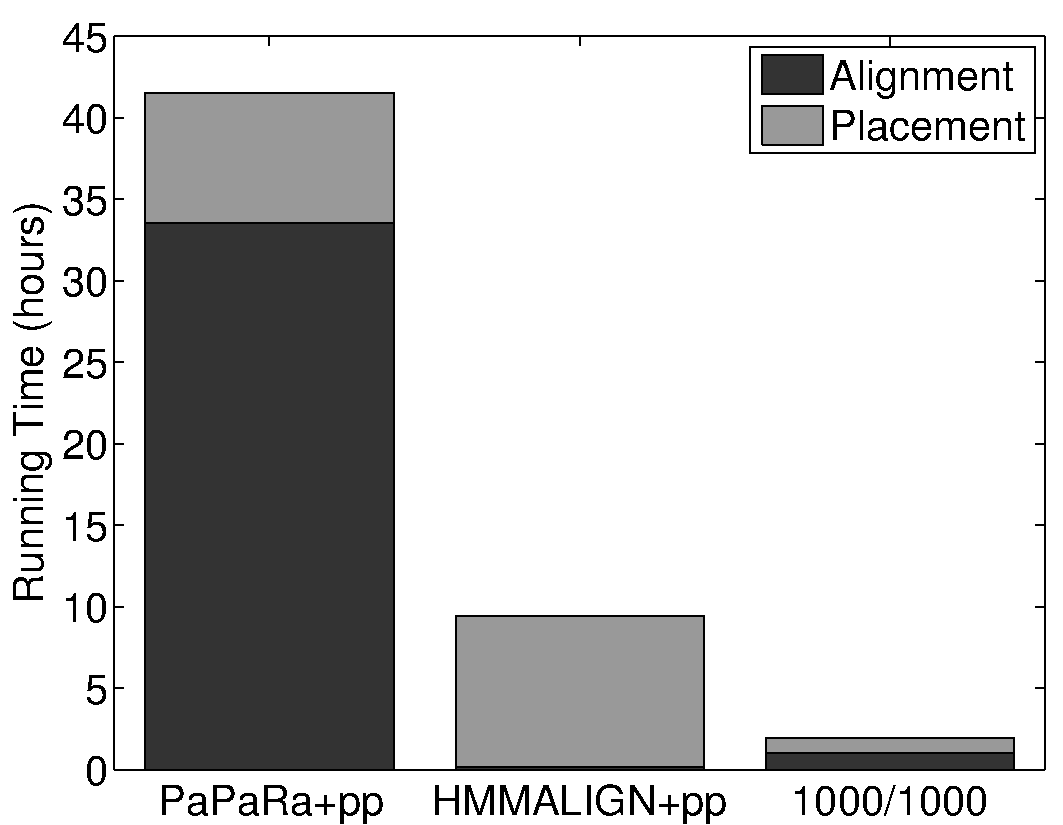
\includegraphics[width=0.35\textwidth]{sepp/bio-time-true}}
\\
%  \subfloat[Peak memory usage using \sate~backbone]
{\label{fig:bms}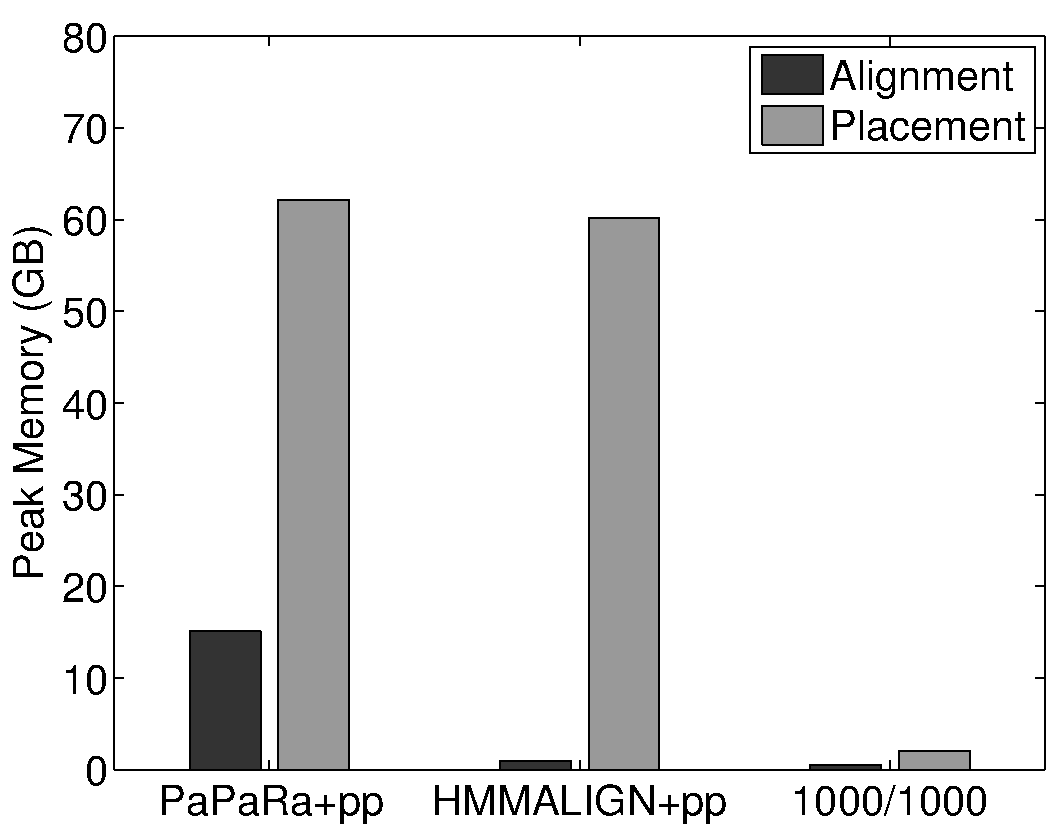
\includegraphics[width=0.35\textwidth]{sepp/bio-mem-sate}}
%  \subfloat[Peak memory usage using curated backbone]
{\label{fig:bmt}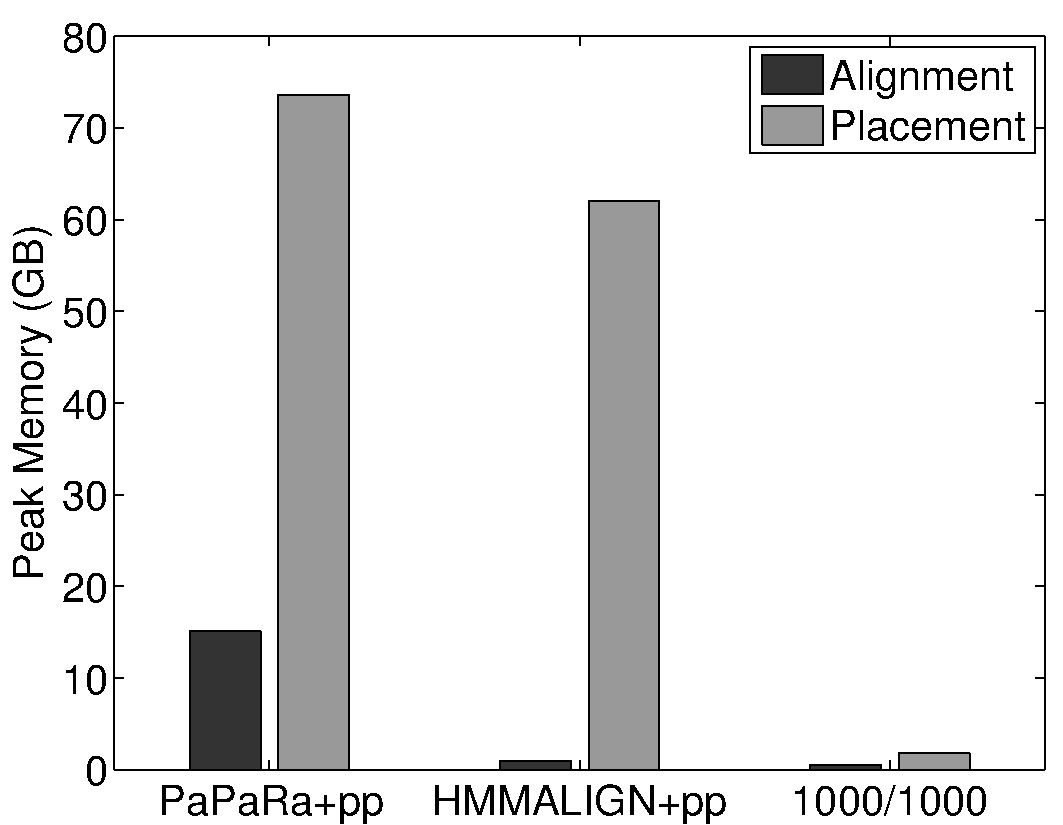
\includegraphics[width=0.35\textwidth]{sepp/bio-mem-true}}
\\
  \subfloat[\sate~backbone]
{\label{fig:bes}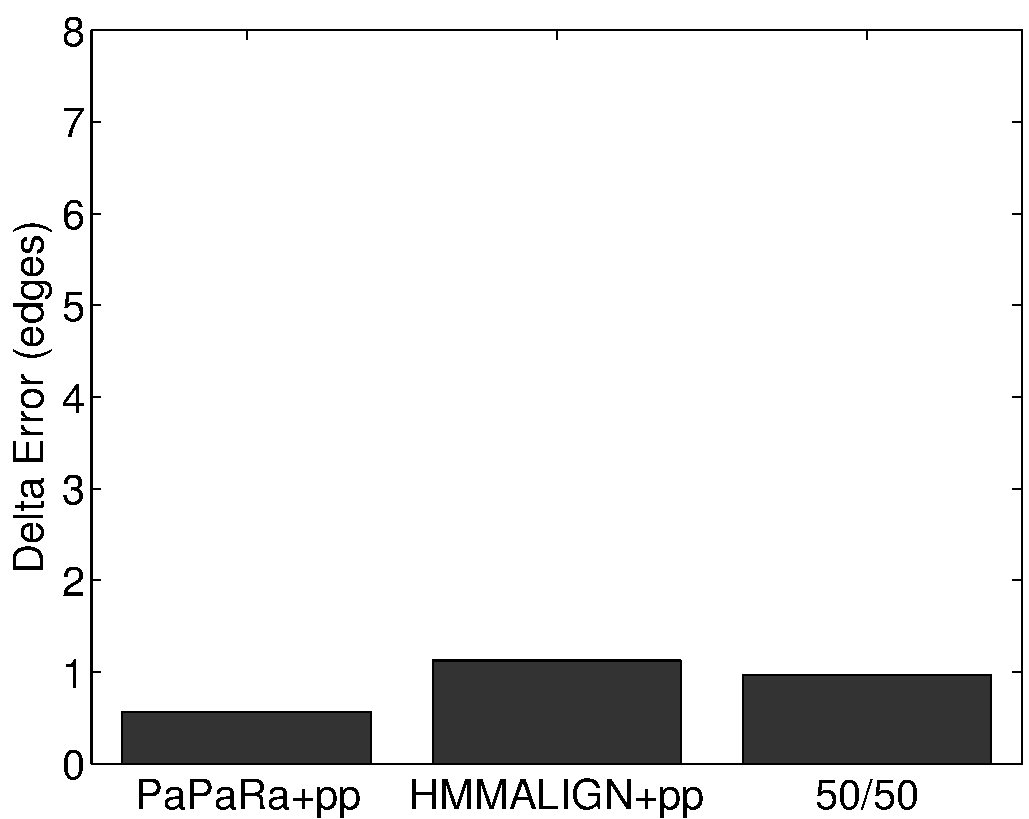
\includegraphics[width=0.35\textwidth]{sepp/bio-err-sate}}
  \subfloat[Curated backbone]
{\label{fig:bio}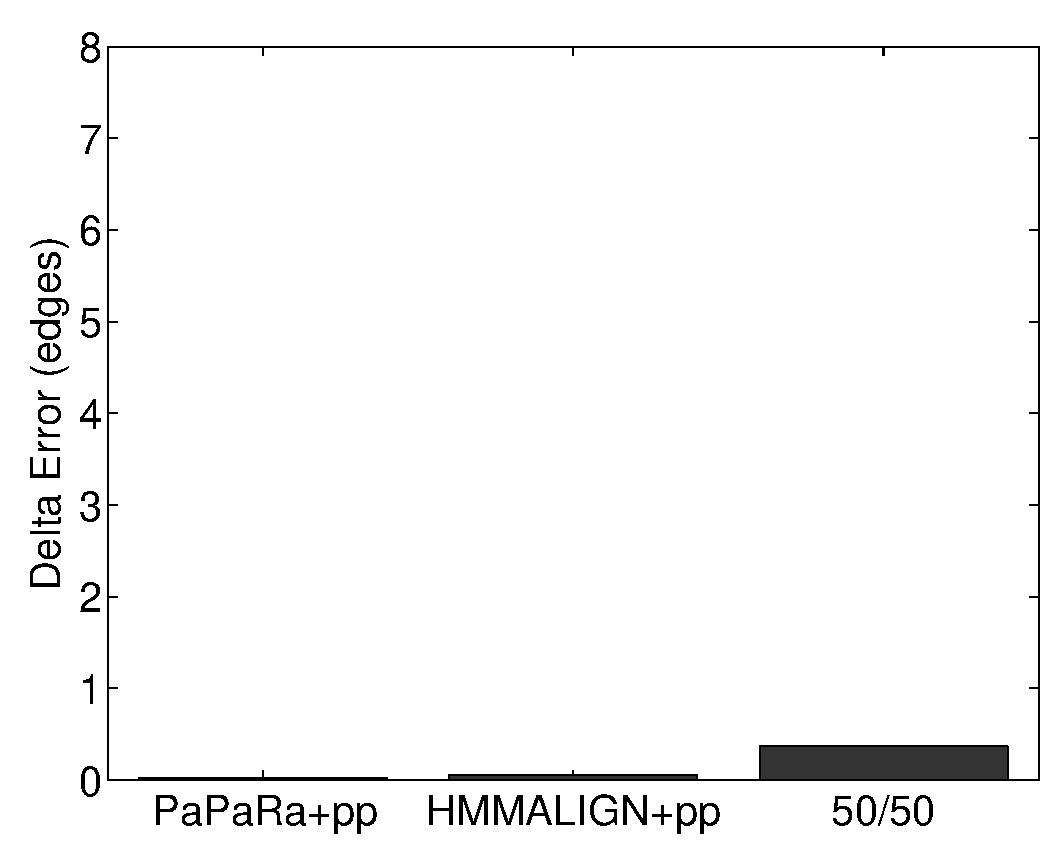
\includegraphics[width=0.35\textwidth]{sepp/bio-err-true}}
  \caption{Results on 16S.B.ALL. I show running time (top), peak memory
usage (middle), and average number of additional missing branches per
query sequence (bottom).  Results for the SAT\'{e} backbone alignment and tree are on the
left, and results for the curated backbone alignment and tree are on the
right. The SAT\'{e} missing branch rate is 7.64\%, and the
missing branch rate for the backbone tree defined by the
true alignment is 1.835\%.  The number of additional missing
branches shown (bottom) is the increment above that amount.}
  \label{fig:bio-all}
\end{figure}

\vspace{.1in}
\subsection{Results on simulated datasets}
The simulated datasets have backbone trees with 500 sequences
and fairly high rates of evolution, with M2 having the highest
rate and M4 having the lowest rate
(Table \ref{tab:datasets}).
Placement error rates were impacted by
the model, 
so that the missing branch rate
for all methods is higher on model M2 than on model M3,
and higher on model M3 than on model M4 (Table \ref{tab:reads-all}).
Not surprisingly, 
 absolute error rates are lower
with the true alignment and tree than with the SAT\'{e}
alignment and tree. 
These trends also held for
PaPaRa and SEPP.


\begin{table}[ht]
\begin{footnotesize}
 \caption{Mean delta-error for all query
sequences. I show the mean delta-error for each method on each model
condition for all the query sequences. 
Count refers to the number of query sequences processed and placed,
HMM refers to HMMALIGN+pplacer,
PPR refers to PaPaRa+pplacer, and SEPP refers to SEPP run in default mode.
}
 \label{tab:reads-all}
\begin{center}
{%
\begin{center}
\begin{tabular}{|l|llll|}
\hline
 & \mc{4}{c|}{ All reads}\\\hline
&bio.&M2   &M3   &M4   \\\hline
&\mc{4}{c|}{ \sate~Backbone}\\\hline
count&13819&99998&99999&99999\\
HMM&1.1&3.4&1.4&\textbf{0.3}\\
PPR&\textbf{0.6}&5.4&3.6&0.4\\
SEPP&1.0& \textbf{1.7}& \textbf{1} &0.4
\\\hline
&\mc{4}{c|}{ True or Curated Backbone}\\\hline
count&13818&99997&99999&99999\\
HMM&0.0&3.2&1.2&\textbf{0.0}\\
PPR&\textbf{0.0}&6.2&3.8&0.2\\
SEPP&0.4&\textbf{1.4}&\textbf{0.7}&0.1
\\\hline
\end{tabular}
\end{center}
}%
 \end{center}
\end{footnotesize}
\end{table}


\begin{table}[ht]
\begin{footnotesize}
 \caption{Mean delta-error for different categories of query
sequences. I show the mean delta-error for each method on each model
condition, as a function of the level of difficulty for the
query sequence, as estimated by HMMER. 
Count refers to the number of query sequences processed and placed,
HMM refers to HMMALIGN+pplacer,
PPR refers to PaPaRa+pplacer, and SEPP refers to SEPP run in default mode.
}
 \label{tab:reads-hard}

\begin{center}
{%
\begin{center}
\begin{tabular}{|l|llll|llll|}
\hline
  & \mc{4}{c|}{ Hard reads} & \mc{4}{c|}{Very hard reads}\\\hline
&bio.&M2   &M3   &M4   &bio.&M2   &M3   &M4\\\hline
&\mc{8}{c|}{ \sate~Backbone}\\\hline
count&104&79510&58924&3989&21&63613&40495&844\\
HMM&2.4&4.2&2.3&\textbf{0.7}&3.9&5.2 &3.2 &1.5\\
PPR&\textbf{0.8}&5.8&4.4&1.0& \textbf{0.9} &6.2 &4.9 &1.5\\
SEPP&2.4&\textbf{2.0}&\textbf{1.4}&0.8& 3.8& \textbf{2.4}& \textbf{1.8}& \textbf{1.0}
\\\hline
&\mc{8}{c|}{ True or Curated Backbone}\\\hline
count&104&79511&58924&3989&21&63614&40495&844\\
HMM&0.5&4.0&2.0&\textbf{0.2}&2.2&5.0&2.9&0.9\\
PPR&\textbf{0.1}&6.7&4.7&0.5&\textbf{0.0}&7.1&5.2&0.9\\
SEPP&1.1&\textbf{1.7}&\textbf{1.1}&0.4&1.5&\textbf{2.0}&\textbf{1.4}&\textbf{0.5}\\\hline
\end{tabular}
\end{center}
}%
 \end{center}
\end{footnotesize}
\end{table}

Figure \ref{fig:M2} and Table \ref{tab:reads-all} show results for
PaPaRa+pplacer, HMMALIGN+pplacer, and SEPP(50,50) (i.e.,
SEPP ran with the default
setting on this model of \ssa~= \ssp~= 50).
Note that SEPP(50,50)
has the lowest delta-error of the three
methods by far, 
followed by HMMALIGN+pplacer,
and then by PaPaRa+pplacer.
Furthermore, the differences are substantial.
The methods are clearly also distinguished by
running time and peak memory usage.
HMMALIGN+pplacer is the fastest, 
SEPP(50,50) is somewhat slower,
and PaPaRa uses much more time.
Both PaPaRa+pplacer
and HMMALIGN+pplacer use more memory than our method.

Results for M3 (see Table \ref{tab:reads-all})
are quite similar to M2, 
with
HMMALIGN+pplacer was much more accurate than PaPaRa+pplacer
and SEPP(50/50) produced more accurate placements
than HMMALIGN+pplacer.  However, the gap between SEPP(50,50) and
HMMALIGN+pplacer was reduced to only half an edge.
On M4 (see Table \ref{tab:reads-all}), however, the relative performance between SEPP(50,50) and HMMALIGN+pplacer depended on
the backbone tree. 
For the SAT\'{e} alignment/tree, SEPP(50,50) was
more accurate but slightly slower than HMMALIGN+pplacer.
For the true alignment/tree, 
HMMALIGN+pplacer was somewhat more accurate and took less
time. However, the difference in placement
accuracy between SEPP(50,50) and
HMMALIGN+pplacer
was extremely small - less than one-ninth of an edge for both
backbones.


\subsection{16S.B.ALL.}  
The datasets based upon  16S.B.ALL,
presented a different kind of challenge.
Each dataset had 13,820 query sequences
and a backbone tree with 13,822 sequences.
Thus, these datasets had much
larger backbone trees, but the backbone trees
and alignments reflected lower rates of evolution.

The default setting for SEPP on this dataset is \ssa~= \ssp~= 1000;
therefore, I ran SEPP(1000,1000) for both backbones.
Results on these datasets are shown in Figure \ref{fig:bio-all}.
Note that PaPaRa+pplacer provides a small
improvement in placement accuracy (slightly more than
half an edge)
in comparison to the other methods.  However, 
PaPaRa+pplacer is enormously computationally intensive, using
40 hours to analyze these data, 
much longer than either other method.
Also,  HMMALIGN+pplacer and PaPaRa+pplacer have
very large peak memory usage, near or above 60GB on both
backbone trees.  Thus, PaPaRa+pplacer is 
computationally extremely intensive, 
and possibly the improvement in placement accuracy is insufficient
given the additional running time costs.

A comparison of SEPP(1000,1000) to HMMALIGN+pplacer
shows that both have extremely good
placement accuracy, with delta-error approximately
one edge for both methods on the SAT\'{e}
backbone tree and well under half an edge on the
curated backbone tree.  
 HMMALIGN+pplacer
produces more accurate placements than our method
for the curated backbone and SEPP(1000,1000) produces
more accurate placements for the SAT\'{e} backbone,
but the differences between the
two methods are small in both cases (less
than a third of an edge).
The methods are, however, distinguished by their
computational requirements, as HMMALIGN+pplacer is
much slower (at least 4 times as much
time) and uses dramatically more memory (60GB as
compared to about 2GB).

\subsection{Comparing methods on query sequences of
different levels of difficulty}

Tables \ref{tab:reads-all} and \ref{tab:reads-hard} compares methods in 
terms of their placement accuracy as a function of 
the level of difficulty in placing the query sequence, as
predicted by HMMER (see the discussion in Section \ref{sec:studydesign}).
Note that error increases as the reads become more difficult,
as HMMER predicts.
I show that SEPP, run in default mode, performs very well
in general (as observed earlier) in comparison to
HMMALIGN+pplacer and PaPaRa+pplacer, but has a
particularly strong advantage on the hard and very hard reads.
Interestingly, PaPaRa+pplacer does well on hard
and very hard reads
for 16S.B.ALL but not on the simulated datasets.

\subsection{Summary}\label{sec:studydesign}
There are several observations we can make. First,
the methods I evaluated for
phylogenetic placement--PaPaRa+pplacer, HMMALIGN+pplacer,
and SEPP methods--often produce placements that are extremely accurate,
increasing the topological error over the input backbone tree
by at most an edge (often much less than an edge) on average.
Furthermore, while these methods do sometimes have 
differences in placement accuracy that go beyond an edge,
these differences are sometimes still
small enough to be relatively unimportant, compared 
to the computational cost
required to obtain the improved placement accuracy.

However, I did observe conditions  in which
the differences in placement accuracy were quite large, suggesting
that increased effort in placing query sequences correctly was
merited.  For example, 
I see big differences in
placement accuracy on model M2, resulting in
several edges improvement produced by SEPP(50,50)
over HMMALIGN+pplacer.
The  conditions under which
accuracy differences are substantial are characterized by large evolutionary
distances between some pairs of full-length sequences.
I conjecture that in such conditions, the HMMs produced by HMMER on
the full set of taxa may
not be sufficient to produce highly accurate alignments for the
query sequences, and will result in degraded placement accuracy.
The technique I introduce here avoids this problem by using HMMER to
produce HMMs
only on smaller, less diverse, subsets of the taxa.  As a result,
the HMMs may produce more accurate alignments to the query sequences,
and result in improved phylogenetic placement.

I note the interesting differences between
HMMALIGN+pplacer and PaPaRa+pplacer.  Only on the slowest evolving
dataset, 16S.B.ALL,  does
PaPaRa+pplacer produces more accurate placements than HMMALIGN+pplacer,
while PaPaRa+pplacer has substantially less accurate placements
for the faster evolving datasets.
This is consistent with the need to estimate transition state
matrices on each edge, an estimation that may only be highly
accurate under sufficiently low rates of evolution.

Furthermore, these methods differ dramatically with respect to
running time, with PaPaRa+pplacer much more computationally
intensive than HMMALIGN+pplacer and the default setting for
SEPP, thus suggesting that PaPaRa+pplacer is unlikely to
be useful in largescale metagenomic analyses.

The comparison between HMMALIGN+pplacer and SEPP is more
complex, because SEPP is parameterized by the two
algorithmic parameters \ssa~and \ssp. Here I see that some
very simple settings for these parameters (\ssa~= \ssp, both set to
about 10\% of the number of taxa in the backbone tree) produces very
fast results with generally very good accuracy, coming close to the
accuracy obtained by the best methods (or improving on them), but
in a fraction of the time.  
Other settings for the parameters can improve the placement accuracy but
require greater running time and memory usage.  


\section{Conclusion and future work}\label{sepp:conclusion}
In this chapter, I presented, SEPP, a general technique for boosting
the accuracy and/or speed of a phylogenetic placement method. 
I show in a simulation study its
performance when coupled with HMMALIGN+pplacer, and showed improvements
in placement accuracy and/or running time. Given the plans to analyze millions of reads, the speed-ups that SEPP provides could be essential to providing scalability for
phylogenetic placement methods.

I plan to explore other methods for estimating the extended alignment.
For example, improved accuracy might be obtained by
coupling SEPP with PaPaRa for those cases where
the backbone tree and alignment has slow evolutionary
rates to enable PaPaRa to produce highly accurate extended alignments.
Another potential method to examine is Mafft-profile~\cite{Katoh2012}.
Mafft-profile takes in a backbone alignment and a sequence of query sequences and aligns each query sequence to the backbone alignment.  Mafft-profile can be run under an accurate setting (``addfragments'' and ``L-INS-I''), however,
the most accurate setting can only be run on a backbone alignment of 1000 sequences.  More accurate placements may be obtained if Mafft-profile is used within SEPP, using the decomposition technique to allow Mafft-profile to scale to larger datasets.

Based on the placement of the query sequence, the evolutionary relationship between the query sequence and the sequences in the backbone alignment can be inferred.  Thus, SEPP can be used to taxonomically identify unknown reads based upon the placement of the sequence in the backbone tree.  In Chapter~\ref{tipp_chapter}, I will show how SEPP fares toward taxonomic indentification and how SEPP can be modified to obtain improved classification accuracy.  Finally, the one of the outputs of SEPP is an alignment of the query sequences to the backbone alignment.  For phylogenetic placement, the individual alignment of each query sequence to the backbone alignment is used to locate the placement, and thus, the query sequences have no impact on each other, both in alignment and placement.  This does not necessarily have to be the case.  In Chapter~\ref{upp_chapter}, I will show how SEPP can be modified for ultra-large alignments and how estimating trees on the entire alignment outputted from SEPP, including all the backbone sequences and query sequences, can result in accurate phylogeny estimation.

\chapter{TIPP: Taxonomic identification and phylogenetic profiling using families of Hidden Markov Models}\label{tipp_chapter}
\index{TIPP@\emph{TIPP}}%

In the previous chapter, I presented SEPP, a method for phylogenetic placement using families of HMMs.  I presented results that show SEPP has improved phylogenetic placement accuracy on evolutionarily divergent datasets.  In this chapter, I will show how SEPP can be used for taxonomic identification, and how SEPP suffers from a high false positive rate under difficult model conditions, such has high rates of sequencing error or sparse taxonomic sampling of the backbone sequences.  I will present TIPP, a modification of SEPP that incorporates statistical support measures to control the precision and sensitivity of classification.  I will show that TIPP classifies more fragments correctly compared to leading taxonomic identification methods, and that TIPP maintains high precision and sensitivity under very difficult conditions.  In addition, experimental results will show that TIPP also improves taxonomic profiling accuracy.  

Section \ref{tipp:motivation} formally describes the taxonomic identification and profiling problem and presents previous work on these problems.  I also show how phylogenetic placement can be applied toward taxonomic identification and profiling and present results on taxonomic identification using SEPP.  In Section \ref{tipp:algorithm}, I describe TIPP, an improved version of SEPP for taxonomic identification and profiling.  In Section \ref{tipp:evaluation}, I describe the simulation study designed to evaluate the performance of TIPP toward taxonomic identification and profiling.  Section \ref{tipp:results}, I present the results comparing TIPP for taxonomic identification and taxonomic profiling.  I show that TIPP outperforms other taxonomic identification methods under difficult conditions and that TIPP generally results in better profiles than leading profiling methods.  Finally, in Section \ref{tipp:conclusion}, I discuss possible ways of improving TIPP, and future studies using TIPP.

\section{Motivation and previous studies}\label{tipp:motivation}
Metagenomic studies of microbial communities commonly generate
millions to hundreds of millions of sequencing reads.  The assignment
of accurate taxonomic labels to these sequences is a critical
component in many analyses, but is
complicated by the fact that the majority of the organisms
found in environmental or host-associated communities cannot be easily
cultured in a laboratory, and an even smaller number have been
sequenced, even partially.  Thus, these commonly encountered organisms
are largely absent from existing databases of known genomes and genes.
Providing taxonomic labels to metagenomic sequences requires
extrapolating the knowledge contained in sequence databases to
previously unseen DNA strings.  Simple similarity-based approaches
(e.g., picking the best database hit as the best `guess' at the
taxonomic label) have been shown to be insufficiently
accurate \cite{closest-blast-hit}, leading to the development of 
new and more sophisticated methods.

Recently developed methods improving
on the simple similarity-based approaches include 
(a) composition-based approaches that rely on
various machine learning techniques 
(Support Vector Machines in
PhyloPythia and PhyloPythiaS \cite{McHardy2007a, Patil2011}, 
Interpolated Markov Models in Phymm 
\cite{Brady2011},
Bayesian models in NBC \cite{Rosen2011}, or neural networks~\cite{SOM2006}) to
classify sequences based on their DNA composition (usually based on
the frequency of short k-mers),
(b)  more sophisticated analyses of
similarity search results (e.g., using least-common-ancestor
aggregation in Megan \cite{Huson2007}, or classifiers built from similarity
search results as done in MetaPhyler \cite{Liu2011d,Liu2011}, 
MetaPhlAn \cite{Segata2012a}, and mOTU \cite{Sunagawa2013}
or protein profiles in Carma \cite{Gerlach2011b}), and
(c) combinations of
multiple approaches (e.g., composition and similarity based approaches
in PhymmBL \cite{Brady2009}).  
Some of these approaches (e.g., most of the
composition-based approaches) can be applied to any DNA sequence,
while others are specific to a reference collection of carefully
selected genes (e.g., MetaPhyler, MetaPhlAn, and mOTU use a collection of
universal or clade-specific marker genes).  These
``marker-gene" methods can
achieve much higher recall than other
approaches~\cite{Liu2011d} for sequences from the marker genes, but 
can only classify a small
fraction of all sequences (namely, those that match the 
selected marker genes). 

Abundance profiling, also called ``phylogenetic profiling", 
seeks to estimate the relative
abundance of the species (or
genera, or families, etc.) within a sequence dataset.
While many methods produce these estimates by characterizing
most (or all) of the sequences in the dataset, marker-based methods
produce these estimates by characterizing only those
sequences that match the marker genes they rely on.
Since the marker genes are supposed to be single
copy and universal, these estimations do not need to
be corrected for the copy number in each genome, or for
missing data. 
However, the restriction to sequences that match the marker genes
has the potential to reduce accuracy since it means only a subset
of the sequences are characterized.

\paragraph{Taxonomic identification through phylogenetic placement.}
One approach toward taxonomic identification is through phylogenetic placement.  The evolutionary relationship between the the query sequence and the backbone sequences can be inferred from the placement location.  For example, in Figure~\ref{tipp:placement}, $Q1$ is placed closest to Species $A1$, and thus, it can be inferred that $Q1$ is more closely related to Species $A1$.  Similarly, $Q2$ is more closely related to Species $A1$ and $A2$ than to Species $B1$ and $B2$.  Thus, one simple technique for identifying a query sequence is to classify it by the LCA of its sibling leaf nodes.  Thus, $Q1$ would be classified as Species $A1$ (its only sibling leaf node is Species $A1$) and $Q2$ would be classified as Genus $A$ (its sibling leaf nodes are Species $A1$ and Species $A2$).  

\begin{figure}[htpb]
\begin{center}
{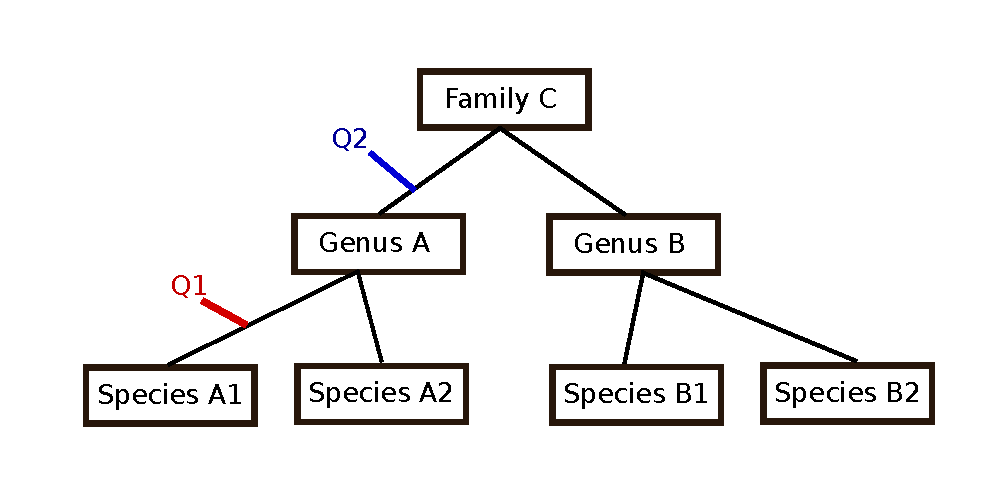
\includegraphics[scale=0.8]{tipp/placement.pdf}}
\end{center}
\caption[Taxonomic classification using phylogenetic placement]{\label{tipp:placement} Taxonomic classification using phylogenetic placement.  The leaf nodes of the rooted backbone tree are labeled with the species name.  Each query sequences is placed onto an edge in the backbone tree and is classified by the LCA its sibling leaf nodes.}
\end{figure}

Using this approach, I compared SEPP and HMMALIGN+pplacer for taxonomic identification under a \emph{leave-species-out} experiment.  Under a leave-species-out experiment, the species of the query sequence is removed from the backbone alignment and tree, simulating the classification of a novel species.  Thus, while the species of the query sequence cannot be correctly identified, the remaining taxonomic lineage (genus, family, etc...) can still be correctly classified.  The fragments were simulated under differring models and rates of sequencing error.  

Figure~\ref{tipp:preliminary_sepp} shows that SEPP is more sensitive than HMMALIGN+pplacer under the hardest model condition (``454\_3''), classifying more fragments correctly, especially at the phylum level.  Both methods tend to classify the large majority of the fragments, leaving very few fragments unclassified.  This results in a very high false positive rate, especially under more difficult conditions.  

To understand why this is the case, it's important to note that pplacer outputs multiple possible locations for the placement of each query sequence.  Each placement has an associated with a likelihood weight ratio.  However, when HMMALIGN+pplacer or SEPP is used for taxonomic classification, only the placement with the likelihood weight ratio is used, ignoring that there may be other placements with almost as high weight.  This was one of the key insights in the development of TIPP.  By taking into account different sources of uncertainty, both in alignment and placement, the false positive rate could be reduced.

\begin{figure}[htpb]
\begin{center}
{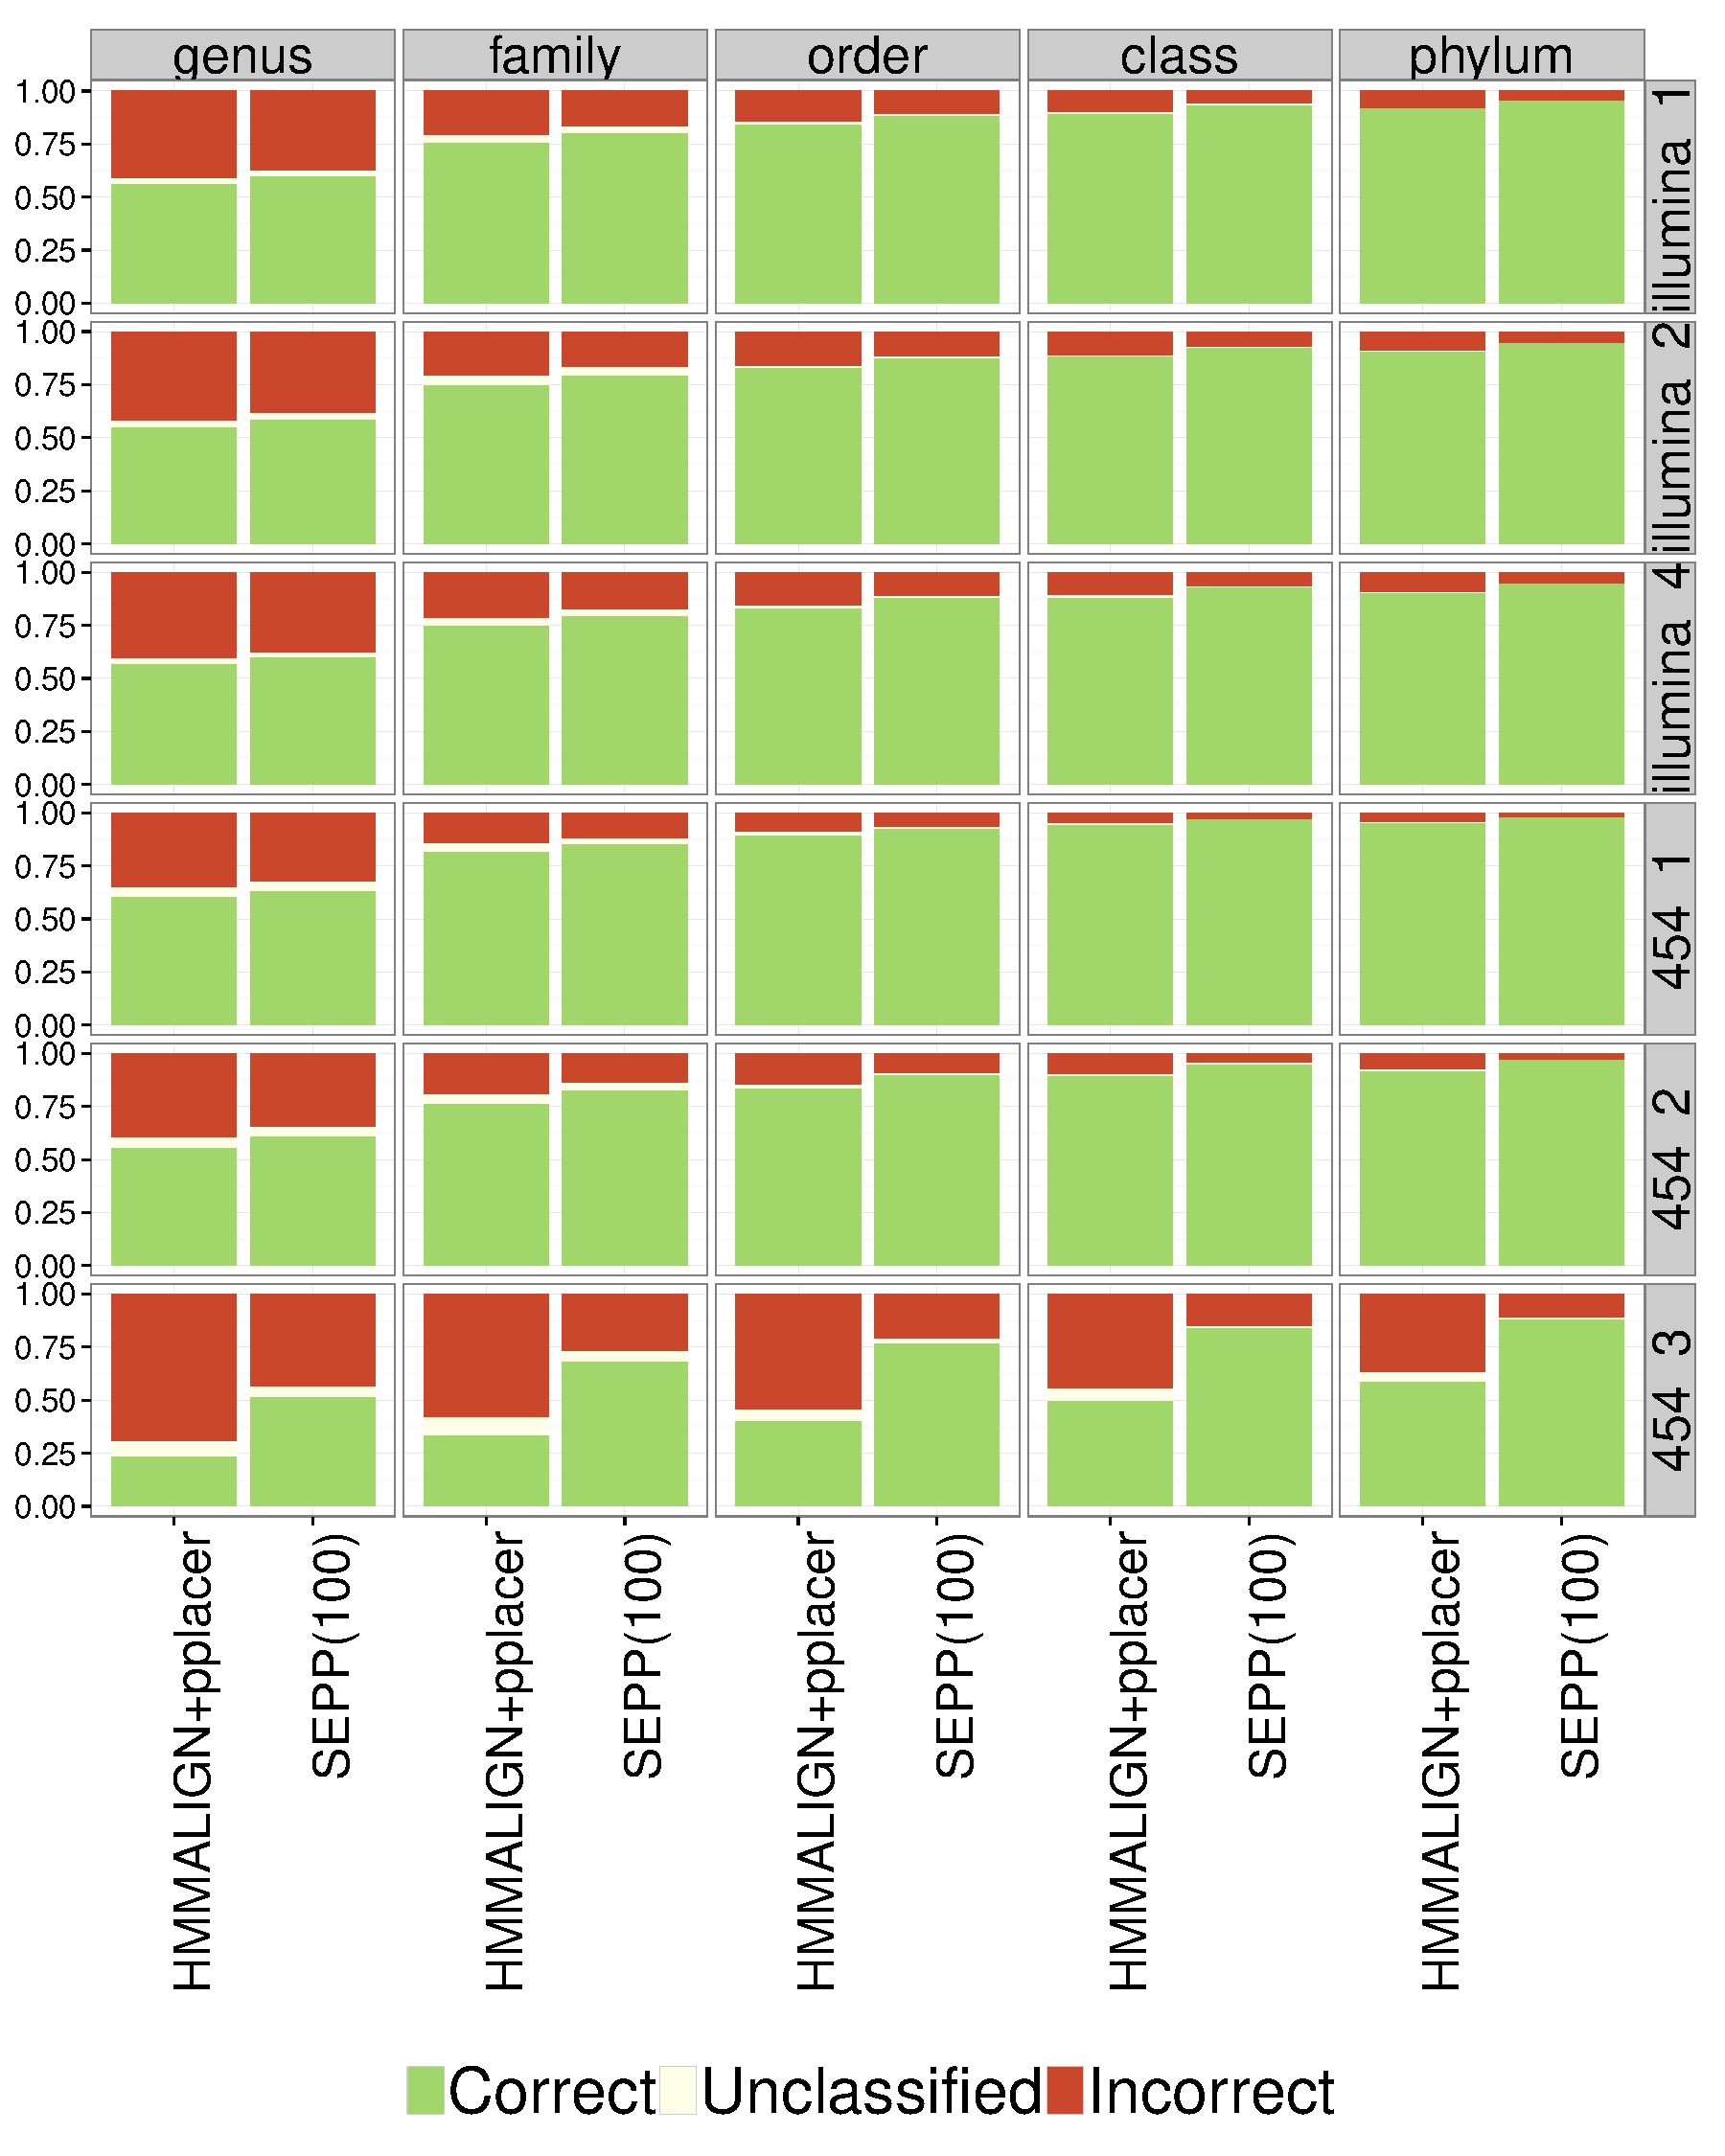
\includegraphics[scale=0.4]{{tipp/sepp.species}.pdf}}
\end{center}
\caption[Comparing SEPP and HMMALIGN+pplacer for taxonomic identification]{\label{tipp:preliminary_sepp} Leave-species-out experiments comparing SEPP and HMMALIGN+pplacer taxonomic classification accuracy on the rpsB gene under sequences simulated under different error model conditions.  Fragments were simulated with either Illumina-like or 454-like errors, and with varying rates of error.  Models denoted with a ``1'' have the lowest rates of error, and models with a ``3'' or ``4'' have the highest rates of error.  SEPP is run using a alignment decomposition size of 100 and placing on the entire backbone tree.}
\end{figure}

%Taxon identification methods only classify a
%subset of the fragments (some correctly and some incorrectly), and
%will leave some fragments unclassified at each taxonomic level.
%Therefore, evaluations of taxonomic classification methods
%consider the percent of fragments classified
%at each rank correctly, incorrectly, or unclassified.  

%However, accurate classifications of just the fragments matching
%marker genes is sufficient for many purposes.
%For example, most culture-independent
%studies of microbial communities have relied on the
%analysis of the 16S rRNA gene.
%These studies, generating broad taxonomic profiles of the
%communities being studied, have been the basis for
%many important discoveries in microbial ecology and
%biomedicine  \cite{Turnbaugh2009}. % Alternative: Aagaard2012, Belda-Ferre2012
%In addition, 
%taxon identification methods should accurately label
%sequences already found in public databases, but should also provide accurate
%guesses on the taxonomy of sequences that are only distantly related
%to known sequences.  In fact, identifying novel organisms or taxonomic
%clades is an important focus of recent studies~\cite{eisen} and taxon
%identification software should be able to accurately identify putative
%novel organisms.  


% We have developed TIPP, a new method for taxon
% identification and phylogenetic profiling.
% TIPP is a marker-based method, but can be used to
% characterize any sequence matching any gene for which
% a dense enough sample of full-length sequences are
% available. In this paper, we explore TIPP using the
% Metaphyler's collection of 30 marker genes.

\section{TIPP algorithm}\label{tipp:algorithm}
TIPP uses a statistical pipeline to 
perform taxon identification, as follows.  
In the first step, TIPP uses BLAST \cite{Altschul1990} to 
determine which sequences map to the marker
genes. 
Then, for each bin of sequences matching a given
marker gene, 
TIPP uses a multi-step statistical technique
to taxonomically characterize each sequence.

For a given bin of sequences mapping to a marker
gene, TIPP uses 
SAT\'{e} \cite{Liu2009,Liu2012} to estimate
the multiple sequence alignment and gene tree
on full length sequences for the marker gene.
It then 
uses SEPP \cite{Mirarab2012}, a highly accurate method for phylogenetic placement
that uses a collection of
Hidden Markov Models (HMMs), 
as implemented in HMMER \cite{Eddy1998},
to insert each metagenomic fragment into the alignment.
For each extended alignment produced in this way,
it inserts the fragment into the taxonomy using maximum likelihood
(implemented in pplacer \cite{Matsen2010} or EPA \cite{Berger2011}).
Each placement of the fragment thus provides a taxon identification of
the fragment, and comes with statistical support values for the
estimated
alignment and taxon placement of
the fragment.  To reduce the potential for
false positive classification (and hence improve the
precision of the taxon identification), TIPP allows the user to
specify minimum statistical support levels for both the alignment and
the placement steps.  Given those thresholds, TIPP computes a
set of alignments and placements that suffices to meet the required
statistical support levels, and returns the LCA (least common ancestor) of these
placements as the final placement. The result is a
statistically-based method that can be tuned for precision or recall,
and which has better recall (even for its more
conservative setting) compared to the other marker-based methods.  

If the desired output is the abundance profile of the
sample, then the taxonomic characterizations obtained
for each bin are pooled, and then the distribution is
estimated from the pooled collection.

\paragraph{\bf TIPP's technique for taxonomic identification for
a single marker gene. }
I now describe in greater detail the 
technique used by TIPP to taxonomically identify the
fragments matching a given marker gene.
The input 
is (1) a set $Q$ of fragmentary
sequences from a single gene,
(2) a set $S$ of
full-length sequences for the same gene, and (3)
a taxonomy $T^*$.
%Since metagenomic samples are a mixture of
%reads from different genes and organisms, 
%TIPP can only be used after
%the metagenomic sample is binned into sets, each of which is
%predicted to come
%from the same gene,
%for which we use BLAST.
%\cite{Eddy1998, Altschul1990,  Langmead2009}.

\noindent{\bf Parameter settings for default TIPP.}
I describe the simplest use of TIPP, which is
used for all cases where $n$, the number of full-length sequences
obtained for the marker gene, is not very large (see Section \ref{supp:large_marker}
 for a description of how I modify TIPP when $n$ is very large).  In this simple version of 
TIPP, I do not constrain the portion of the taxonomy
into which the fragment can be inserted.  I also need to set
$m_a$, the maximum alignment size, whether EPA or pplacer is used,
and the statistical support thresholds $s_a$ and
$s_p$ for alignment and placement support, respectively.

I now describe how TIPP performs
a taxonomic identification of a single query sequence $q$:

\noindent{\bf Step 1: Decomposition.}   TIPP uses a SAT\'{e}
alignment and tree on the set $S$ of full
length sequences as the reference alignment $A$ and tree $T$.  I decompose the
reference alignment $A$ and tree $T$ 
into alignments subsets with at most $m_a$ leaves each as follows.  
TIPP finds a centroid edge in $T$ (one that
separates the leaf set into two sets of
approximately equal size), and breaks the tree accordingly into two subtrees.
For each resulting subtree that contains more than $m_a$ leaves, 
TIPP recursively repeats this decomposition.
This produces a partition of $S$  into subsets $S_1, S_2, \ldots, S_k$,
each of size at most $m_a$.

\noindent{\bf Step 2: Compute Extended Alignment. }  
For a given alignment subset of sequences $S' \subset S$, 
I define $A'$ to be restriction of alignment $A$ to $S'$.
TIPP uses HMMER to compute an HMM $H'$ on $A'$ for each alignment subset
and to score $q$ with respect to each $H'$.
Thus, TIPP represents the backbone alignment with a set of
HMMs (a technique I call an ``HMM
Family").
HMMER produces measures of the fit between
each HMM and each query sequence called ``bit-scores" (discussed in
Section \ref{tipp:bitscores}
).  Then, for query sequence $q$, 
one or more alignment subsets are selected so that total statistical support for the alignments 
is at least $s_a$ (see Section \ref{tipp:bitscores}
for how TIPP uses the ``bitscores" returned by
HMMER in order to compute the statistical support for extended alignments).  TIPP uses HMMER to align $q$ to each of the selected alignment subsets, and
then extends the reference alignment $A$ on the full dataset to include each alignment of $q$.
These are the ``extended alignments" for the query $q$;
thus, each query sequence $q$ gives rise to potentially many different extended
alignments, each with $|S|+1$ sequences.

\noindent{\bf Step 3: Placement.}  
For each extended alignment, 
I use the selected method (EPA or pplacer) to place
$q$ into the refined taxonomy.
I thus obtain multiple placements and their likelihood weight ratios
(a value computed by pplacer and EPA,
which I treat as probabilities) for each extended alignment.
I combine all placement results of different extended alignments, and normalize the
placement probabilities across results from all extended alignments.
%{\bf (optionally weighting placements of each extended alignment by their alignment probability)}.
This results in  multiple placements and their 
associated probabilities for each placement for the fragment. 

\noindent{\bf Step 4: Classification.} 
I assign the statistical support to each node in the taxonomy
by adding the probabilities of all 
placements at or below the edge above the node;
this allows us to
classify the fragment at all taxonomic levels for 
which it has  support of at least $s_p$. 
If $s_p>0.5$ then
this yields a unique taxon identification; otherwise,
TIPP outputs multiple identifications, along with their support. 
The fragment is left unclassified at levels where 
support of $s_p$ is not reached.

Thus, TIPP has many  algorithmic parameters, some
determining how the decomposition is run, and others
determining the statistical support thresholds (one
for the set of extended alignments and one for the
set of
taxonomic placements) and
the taxonomy that is used.
In my experiments,
I use either the NCBI or the RDP taxonomy
(depending on the dataset),
restricted to the species in $S$, 
SAT\'{e} to produce the reference
alignment and tree on $S$, and RAxML to refine the
specified taxonomy with respect to the SAT\'{e} alignment.

\section{Performance evaluation}\label{tipp:evaluation}
I initially evaluated the impact of 
algorithmic parameters on taxonomic classification and
phylogenetic profiling, based on which I
selected default settings for TIPP; these are
reported in the Appendix.
%NAM:  Add in tipp appendix
I then evaluated TIPP in comparison 
to other phylogenetic profiling methods on
a collection of datasets. 
However, I also 
performed experiments evaluating the impact
of sequencing error on taxonomic classification,
of TIPP's
algorithmic parameter settings on the
taxonomic identification, and finally
on the ability of different taxonomic classification
methods to identify ``dark matter" (i.e., sequences
that come from novel phyla). 

\paragraph{\bf Methods studied. }
I compared MetaPhyler, MetaPhlAn, PhymmBL, and NBC as abundance profiling methods.  
TIPP, MetaPhyler, and MetaPhlAn are marker-based methods and can classify fragments from their marker reference dataset.  TIPP and MetaPhyler use the same set of universal 
housekeeping markers that are unlikely to undergo duplication and horizontal gene transfer.  MetaPhlAn, on the other hand, selects markers that uniquely identify specific taxonomic groups.  NBC and PhymmBL are composition-based methods and can classify fragments originating from any region in the genome.

MetaPhyler classifies every
fragment at each taxonomic level and assigns
the classification a confidence score;
For MetaPhyler, I use a version that
classifies a fragment at the 
most specific classification yielding a confidence 
score of 90\% or higher.  
I used MetaPhyler version 1.25 
(downloaded from \url{http://metaphyler.cbcb.umd.edu}), 
an extension of the originally published algorithm that also provides a 
confidence for each classification.  
The chosen confidence cutoff of 
90\% roughly corresponds to a mis-classification 
rate of 10\%, chosen as a reasonable trade-off between precision and recall.  
For PhymmBL, I classify a fragment at the most 
specific classification yielding a confidence score 
of 95\% or higher;  however, PhymmBL does not 
give confidence scores at the species level, and so 
cannot be used to perform taxonomic identification and 
abundance profiling at the species level.  
Finally,  NBC gives a confidence score of the fragment matching to a genome.  I accept the classification if the confidence score is above the species threshold suggested by the NBC authors.  Thus, a fragment will either be classified at the species level or be completely unclassified.  See Section \ref{supp:commands} 
for commands used for training and running these methods.

Except where indicated, I used the
following ``default" settings for TIPP. 
The 
alignment subset size $m_a$ is
set to 100,
and I place fragments into
the refined taxonomy
(described above)
after I compute the extended alignments.
%run many experiments and assess
%the impact of changing parameter settings.
In all experiments shown here I use
pplacer for the placement step (see Section \ref{tipp:tipp.epa.pplacer.sec} 
for results on using EPA inside TIPP).
The remaining parameters are the alignment subset size $m_a$
and the alignment and placement support thresholds $s_a$ and $s_p$,
respectively. I refer to TIPP with this parameter setting by TIPP($s_a,s_p,m_a$).  All results shown in this paper use 95\% as the alignment and placement support threshold.

%Siavash - no fragments simulated for the 16S sequences
%in the non-leave-one-out experiments?
%That's correct, we only had leave-one-out experiments for 16S
%TIPP(50\%,100) and TIPP(95\%,100) were run on these datasets.
\paragraph{\bf Reference marker datasets. }
In order to classify metagenomic samples, 
TIPP uses the reference 
sequence dataset obtained from \cite{Liu2011d,Liu2011},
which consists of  30 phylogenetic marker genes that span the Bacteria and Archaea domains.  
The marker genes selected were believed to be single 
copy genes and universally present across the Bacteria domain, 
making them resistant to horizontal gene transfer 
and gene duplication.  
Only species whose genomes have been sequenced were 
present in the reference dataset.  The number of 
sequences in each marker ranges from 65 to 1555 sequences, 
with an average of 1312 sequences per marker gene.  
See Section \ref{tipp:marker_genes} 
for the list of marker genes and 
the empirical statistics of the reference
alignments on these datasets. 

%The reference dataset was enhanced by including sequences from the 16S gene.  The 16S sequences were separated into two different sets, the 16S bacteria set, containing 9197 sequences, and the 16S Archaea set, containing 375 sequences.  16S sequences were downloaded from the RDP database~\cite{Cole2009}.  Only high quality 16S sequences longer than 1200 bps from species-type 
%strains cultured from individual isolates were used.

\paragraph{\bf Simulated taxonomic identification datasets. }
Datasets used in the taxonomic identification experiments were generated by 
simulating fragments from biological data and then adding errors 
for either Illumina or 454 sequencing technologies, varying the error rates from low to high.  I used MetaSim \cite{Richter2008} to generate fragments with Illumina or 454 errors, starting from the reference datasets of
 30 marker genes and the 16S gene.  Both 100-bp Illumina-type fragments and 
300-bp 454-type fragments were generated, with different levels of error, thus, I have Illumina\_1, Illumina\_2, and Illumina\_4 models, and
454\_1, 454\_2, and 454\_3 models (in the increasing order of error rates).
Illumina-type fragments contained only substitution errors,
and  454-type fragments contained only indel errors, 
biased toward insertions.  

These error models allow us to  explore 
the impact of varying sequencing error on taxonomic
identification, and the higher error models
improves the 
realism of the non-leave-out experiments.
These error models range from low amounts of error,
with the default average number of error 
events per fragment, up to 7.6 times the 
average number of substitutions per fragment (for Illumina data)
and up to 4.2 times the number of indels (for 454 data);
see the Table \ref{tipp:metasim_stats} 
for
the fragment 
statistics for the different error models.   
Current sequencing  data, \emph{when
properly filtered}, do not exhibit the
levels of error shown in the highest error
model conditions
(Illumina\_4 and  454\_3); therefore,
this experiment 
represents a stress test
of the methods, testing
robustness to increased
error in the data, that
may indicate performance under future
sequencing technologies, or under unfiltered data.

In total, 
the leave-one-out experiments
had 600,000 fragments simulated from the 30 marker genes and 240,000 
fragments were simulated from the 16S genes.
The non-leave-one-out experiments had 600,000 fragments simulated 
from the 30 marker genes.

\paragraph{\bf Simulated abundance profiling datasets. }
I used several datasets from previous studies in the abundance profiling experiments.  
The simulated abundance profiling datasets can be grouped by the complexity of the abundance profiles and the average fragment length.  High complexity (HC) datasets have 
roughly uniform distributions of the species.  
Low complexity (LC) datasets have staggered distributions 
of the species; typically low complexity distributions have a 
power law distribution.  Medium complexity (MC) datasets fall in between LC and HC datasets.  Datasets either have short average read length 
(at most 100 nucleotides) or long average read length (200-1000 nucleotides).  
I used simulated abundance profile datasets from 4 different studies: the MetaPhlAn HC and LC datasets~\cite{Segata2012a}, the FACS HC dataset~\cite{Stranneheim2010}, the FAMeS LC, MC and HC simulated datasets~\cite{Mavromatis2007}, and the WebCarma HC dataset~\cite{Gerlach2011b}.  
Of these datasets, only the MetaPhlAn datasets had short sequences.
To better examine performance on datasets with short sequences, 
I generated Illumina-like reads from the genomes used in the WebCarma and FACS datasets.  Finally, the FACS dataset originally contained both human and viral sequences.  These were removed from the datasets so that profiling performance was tested only on bacterial and archaeal sequences.  Table~\ref{table:overview} shows the summary of the datasets examined.  A more in-depth description of the datasets can be found in Section \ref{tipp:datasets}
.

\begin{table}[hptb]
\caption{\label{table:overview}Summary of all simulated abundance datasets.  Complexity refers to the distribution of species in the profile.  High complexity datasets have an even distribution of species.  Low complexity datasets have a staggered distribution of species.  Medium complexity datasets fall in between.  Datasets with a ``*'' were generated by generating Illumina-like reads from an existing abundance profile using MetaSim.  Datasets labeled with ``DOE-JGI'' used fragments generated from genome sequencing projects at the Department of Energy Joint Genome Institute.  
``Length" refers to the average length of the reads, and ``Complex." refers to the 
complexity (High, Medium, or Low). 
%The parameter $n$ refers to the number of genomes,
%$k$ refers to the average sequence length, and ``Complex." refers
%to the level of complexity (High, Medium or Low).
}
\begin{center}{
\scalebox{0.8}{
\small
\begin{tabular}{|l|r|r|r|r|r|}
\hline
Dataset& \# Genomes & Complex. & Seq. Model & Reads & Length \\ %&Source\\
\hline
MetaPhlAn HC& 100 & High & NA & 1000000 & 88 \\ %&\cite{Segata2012a}\\
MetaPhlAn LC& 25 & Low & NA & 240000 & 88 \\ % &\cite{Segata2012a}\\
FAMeS HC& 113  & High & DOE-JGI & 116771 & 949 \\ %&\cite{Mavromatis2007}\\
FAMeS MC& 113  & Medium & DOE-JGI & 114457 & 969 \\%&\cite{Mavromatis2007}\\
FAMeS LC& 113  & Low & DOE-JGI & 97495 & 951 \\ %&\cite{Mavromatis2007}\\
FACS HC & 19 & High & 454 & 26984 & 268 \\%&\cite{Stranneheim2010}\\
FACS HC Illumina& 19 & High & Illumina & 300000 & 100 \\%&\cite{Stranneheim2010}*\\
WebCarma & 25 & High & 454 & 25000 & 265 \\ %&\cite{Gerlach2011b}\\
WebCarma Illumina& 25 & High & Illumina & 300000 & 100 \\%&\cite{Gerlach2011b}*\\
\hline
\end{tabular}}}
\end{center}
\end{table}

\paragraph{\bf Taxonomies. }
The taxonomic trees for the 30 marker genes were estimated by 
using RAxML \cite{Stamatakis2006} to refine the NCBI taxonomy using 
the SAT\'{e} alignment of the reference datasets (i.e., the reference
alignments).
The taxonomic trees for the 16S RNA gene were estimated by 
using RAxML to refine the RDP taxonomy using 
the reference SAT\'{e} alignment.  

Taxonomic identification results presented in this paper are based on reads simulated from 32 marker genes (30 genes used in the MetaPhyler study and two additional 16S marker genes).  Note the marker-based methods TIPP and MetaPhyler are trained specifically on this reference dataset.  Thus, the main 
foci of the taxonomic identification experiments are parameter exploration for TIPP and 
the comparison of TIPP versus MetaPhyler.

\paragraph{\bf Experiments. } 
I performed both \textit{leave-one-out} experiments and \textit{non-leave-one-out} experiments.  In \textit{leave-one-out} experiments, a particular taxonomic group is removed from the reference set, 
and   then fragments belonging to the left-out taxonomic group are classified using various tools.  In \textit{non-leave-one-out} experiments, the fragments being classified are obtained by adding sequencing errors to short substrings from the full-length sequences.  

%For example, in leave-out-species experiments, all sequences belonging to the species of the query fragment were removed from the reference dataset.  While it is impossible to correctly identify the species for fragments, it is still possible to classify the remaining taxonomic ranks correctly (genus, family, and so forth).  Therefore, in a leave-out-species experiment, we report results for classification at levels above the species, but not at the species level.

%By controlling the error rates, we can explore the ability of methods to perform taxonomic identification on fragments from organisms either very similar (fragments under low error models) or very dissimilar (under high error models) to those in the reference database.   

The leave-one-out experiments are useful at understanding whether methods are able to identify novel organisms or taxonomic clades (an important focus of recent studies~\cite{eisen}). However, the non-leave-one-out experiments (especially under the higher error models) are useful at understanding how well methods are able to identify sequences from organisms with close relatives in public databases.  Thus, evaluating performance under both conditions is helpful at characterizing how well the methods work.  Real metagenomic samples are likely a mix of species, only some of which are not present in the reference datasets, and therefore will fall somewhere in between the two extremes of leave-one-out and non-leave-one-out in terms of ease of classification.

Abundance profiling results presented in this paper are based on reads simulated from 
metagenomes.  Abundance profiles for each method were estimated by examining the set of fragments classified by the profiling method.  
As noted earlier, marker-based methods require the 
fragments to first be binned to the reference markers.  
%The choice of the binning method can have a profound impact on the final estimated profile; however, studying the impact of the binning method is outside the scope of this study.  
%BLAST \cite{Altschul1990} was 
%used as the default binning method for all marker-based methods.  
BLAST is used internally by MetaPhyler and MetaPhlAn with 
settings specific to the software; the BLAST setting used by TIPP can be found in Section \ref{supp:commands}
.

MetaPhlAn and MetaPhyler both output an abundance profile from a set of sequences.  All other methods studied output the classification of the fragments; abundance profiles for these methods were estimated by using the relative abundance of the fragment classification results.  Abundance profiles for all methods were then normalized by including only fragments that were classified at the taxonomic level of interest.  For example, species-level abundance profiles are computed only on fragments that have species levels classification; fragments left unclassified at the species level are excluded.  Details on the computation of the abundance profiles can be found in Section \ref{supp:profile_estimation}
.

\noindent{\bf Experiment 1: Algorithmic parameter exploration. }
TIPP has many several parameters, and so my initial experiment
evaluated the impact of these parameters on the sensitivity and
precision of 
TIPP used as a taxon identification method, and then on the
accuracy of the phylogenetic profiles it produces. I set
default values for these parameters based on these initial experiments.

\noindent{\bf Experiment 2: Abundance profiling experiments.}
I performed abundance profiling experiments, separating the datasets into two different groups: datasets with short reads (88-100 bps) and datasets with long reads (265-969 bps).  
I explored performance on  datasets with uniform (HC datasets) and staggered distributions (MC and LC datasets) of species.  

\noindent{\bf Experiment 3: Evaluating
the impact of sequencing error on taxonomic identification  methods.}
I performed a non-leave-one-out simulation study 
to compare NBC, PhymmBL, and MetaPhyler to TIPP on taxonomic identification of fragments simulated from marker genes (MetaPhlAn was excluded because it uses a disjoint reference set), evaluating the
impact of sequencing error on taxonomic classification.

\paragraph{\bf Performance evaluation. }
For the taxonomic
classification methods, the true lineage of each fragment is known, 
so I compute the  percentage of fragments classified correctly, incorrectly, and left unclassified at each taxonomic rank.

For the abundance profiling experiments, the true abundance 
of the metagenomes is known, so I
compute  the root-mean-squared error 
($RMSE$) of the estimated taxonomic profile. 
Let ${C_l}$ be the set of clades found in the true profile and all the estimated profiles for the taxonomic level $l$, $R_x$ be the abundance of clade $x$ for the reference profile, and $E_x$ be the abundance of clade $x$ for the estimated profile.  Then $RMSE_l$ (root-mean-squared-error for a taxonomic level $l$) is:

\begin{equation}
%MSE_l = (\sum_{x\in{C_l}} \frac{(R_x-E_x)^2}{|x|})^{\frac{1}{2}}\\
RMSE_l = \sqrt {\sum_{x\in{C_l}} \frac{(R_x-E_x)^2}{|C_l|}}\\
\end{equation}

\noindent
I normalize the $RMSE$ by TIPP(0\%,0\%,100)'s $RMSE$ to infer the relative performance of the methods.  

\section{Results}\label{tipp:results}
\noindent{\bf Experiment 1: Parameter Exploration Experiments.}
Initial experiments evaluated the impact of the
algorithmic parameters (support thresholds, alignment subset size,
and placement subset size) on TIPP for fragment taxon identification 
(Sections S5.1 and S5.3)
and phylogenetic profiling (Fig. S15 and S16).
%(Sections \ref{supp:leave_out_tipp_variant} and \ref{supp:tipp_non_leaveout_variants})
%and phylogenetic profiling (Fig.~~\ref{tipp:profile_short_tipp_compare} and 
%\ref{tipp:profile_long_tipp_compare}). 
%These results are provided in the
%Supplemental Materials, but show the following basic trends.
%We begin with the results of a leave-one-out comparison of five TIPP variants.  These versions of TIPP are obtained by different settings for the
%alignment support  (0 or 95\%), placement support (0 or 95\%),
%and placement subset size (1000 or ALL). Note that 
%TIPP(0\%,0\%,ALL) is identical to HMMER+pplacer, and
%TIPP(0\%,0\%,100) is identical to SEPP. Thus,
%this experiment also gives a direct comparison 
%between TIPP, SEPP, and HMMER+pplacer.
%Due to the computational difficulty of running the leave-one-out
%experiments, we ran TIPP with alignment subsets of size 100.
%Here, we show the leave-out-species results (see Figure~\ref{tipp:leave_out_tipp}), but
%the Appendix also includes results for other levels. The Appendix also
%includes precision and recall measures, statistical tests, and results in tabular format.
The results show that using 0\% for both the
alignment and placement support thresholds
increased the sensitivity substantially, but also
decreased the precision; thus, more fragments were
classified at each level, but some of these classifications
were incorrect, compared to using a threshold of 95\%.
%TIPP(0\%,0\%,ALL) and TIPP(0\%,0\%,100) % (hmmer+pplacer and SEPP respectively)
%have very high false classification rates.
%The comparison between TIPP(0\%,0\%,ALL) and TIPP(0\%,95\%,ALL) shows
%that increasing the placement support from
%$0\%$ to $95\%$
%dramatically reduces the
%false classification rate while only
%modestly reducing the true classification rate
%(precision and recall differences are all statistically significant with p-values $< 0.02$; see Appendix).
%The comparison between
%TIPP(0\%,0\%,ALL) and TIPP(0\%,0\%,100), or 
%TIP(0\%,95\%,ALL) and TIPP(0\%,95\%,100),
Using an HMM Family rather than a single HMM
%shows that decomposing to subsets of size 100 
increases the true classification rate and reduces the
false classification rate, with the 
biggest improvements observed for lower 
taxonomic levels under the higher error conditions.
%Comparing TIPP(95\%,95\%,100) and TIPP(0\%,95\%,100) 
%shows that
%considering alignment support also 
%improves precision, but at a reduction in
%recall.  
%Overall, TIPP(95\%,95\%,100) has
%the lowest false classification rate of these
%variants, while still classifying a large portion of fragments.
%The choice between TIPP(95\%,95\%,100) and TIPP(0\%,95\%,100)
%needs to be made based on the relative importance
%of recall and precision, and thus depends on the specific application.
 TIPP(95\%,95\%,100)
(that is, alignment and placement support threshold of 95\%, and
using an HMM family with alignment subsets of size 100) is
the default setting for TIPP when used as
a taxonomic classifier for individual reads.
Interestingly, when the objective is to estimate
the phylogenetic profile (i.e., the distribution of
taxa within a dataset, for
some specific taxonomic level), then reducing the
alignment and
placement support thresholds improves the estimated distribution.
That is, the increase in true positives (sequences that 
are correctly classified)
is sufficiently larger than the increase in false positives 
(sequences that are incorrectly classified), so that the
resultant distribution that is estimated has higher
accuracy.
Thus, for the purpose of estimating phylogenetic
profiles, we used TIPP(0\%,0\%,100) as the default setting.
For full details on these experiments, see the Supplementary materials.

\begin{table}[hptb]
\caption[The normalized average $RMSE$ for abundance profiling methods.]{\label{tipp:table_abundance}
The average $RMSE$ on the short and long fragment datasets, normalized by TIPP's $RMSE$ for each model condition and each taxonomic rank.  Thus methods with $RMSE>1$ have worse performance than TIPP, and methods with $RMSE<1$ have better performance than TIPP.  Note 
that PhymmBL does not output any species level classifications.
We use 
TIPP(0\%,0\%,100) for abundance profiling (see SOM for results
using other variants).
The best results for each level and 
fragment length are in boldface.}
\begin{center}
\scalebox{.80}{
\begin{tabular}{|l|r|r|r|r|r|r|}
\hline
 Short &&&&&&\\
Fragments&Species&Genus&Family&Order&Class&Phylum\\
\hline
NBC&1.595               &1.991          &2.435         &2.440         &2.038&2.661\\
PhymmBL&NA              &1.993          &2.403         &2.386         &1.934&2.487\\
MetaPhlAn&\textbf{0.931}&1.029          &1.128         &1.184         &1.103&1.333\\
MetaPhyler&6.143        &3.642          &2.310         &1.604         &1.460&1.278\\
TIPP&1.000              &\textbf{1.000} &\textbf{1.000}&\textbf{1.000}&\textbf{1.000}&\textbf{1.000}\\
\hline
 Long &&&&&&\\
 Fragments&Species&Genus&Family&Order&Class&Phylum\\
\hline
NBC&1.161          &1.250         &1.264         &1.236         &1.059&1.888\\
PhymmBL&NA         &1.194         &1.075         &1.045         &\textbf{0.823}&1.373\\
MetaPhlAn&1.802    &1.372         &1.202         &1.168         &0.986&1.463\\
MetaPhyler&4.582   &1.779         &1.343         &1.228         &1.239&1.520\\
TIPP&\textbf{1.000}&\textbf{1.000}&\textbf{1.000}&\textbf{1.000}&1.000&\textbf{1.000}\\
\hline
\end{tabular}}
\end{center}
\end{table}

\noindent{\bf Experiment 2: Abundance profiling experiments.}
We show results comparing TIPP to NBC, PhymmBL, MetaPhlAn, and Metaphyler 
 in Table~\ref{tipp:table_abundance} (see Tables S21 and S22 for results on individual datasets). 

On the short fragment datasets, 
methods differ on particular datasets,
and some datasets are harder than others
(for example, MetaPhlAn-LC
presents a more difficult challenge than MetaPhlAn-HC).
MetaPhyler's accuracy is extremely poor at the more
specific levels, and has among the worse accuracy at the species and genus level.
MetaPhlAn has the best accuracy at
every level on the two MetaPhlAn datasets (MetaPhlAn HC
and MetaPhlAn LC).
TIPP is the best on the WebCarma Illumina dataset at every
level.
On the FACs HC Illumina dataset,
 TIPP is also best on the lower levels (species through
order),
MetaPhlAn is best at the class level, and
MetaPhyler is best at the phylum level.
Averaging across these four datasets, 
TIPP and MetaPhlAn have the best results of all methods, and
are very close in performance (MetaPhlan
is better at the species level,
slightly less accurate than TIPP at the genus level,
and less accurate than TIPP at the family through class levels) with 
the exception of the phylum level (MetaPhlan has 33.3\% worse RMSE).

On the long fragment sequences, 
the absolute and relative performance of methods can differ
substantially between datasets.
TIPP has the best accuracy at all
levels except for class (where MetaPhlan is 
best) for the FACs HC dataset.
On the FAMeS HC dataset,
MetaphlAn is generally best, but 
NBC is best at the species level.
On the FAMeS LC dataset, NBC and TIPP are competitive for the best at
the species and genus level, but PhymmBL is best at the
other levels.
On the FAMeS MC dataset, TIPP is best at the species, genus,
and phylum levels, but MetaPhlAn is best at the other levels.
Finally, on the WebCarma dataset, NBC is best (or close to the best)
at the species and genus  levels, PhymmBL is 
best at the family through class levels,
and TIPP, PhymmBL, and MetaPhlAn are the best at the 
phylum level.
Examining average performance by level,
I see the following trends.
At the species level, TIPP has the best average 
performance, NBC is second (16.1\% worse than TIPP), 
and MetaPhlAn is third (80.2\% worse than TIPP).
At the genus level, TIPP is best, PhymmBL is
second (19.4\% worse than TIPP), and NBC is third (25.0\% worse than TIPP).
At the family level, TIPP is first, PhymmBL is
second (7.5\% worse than TIPP), and MetaPhlAn is third (20.2\% worse than TIPP).
At the order level, TIPP is first, PhymmBL is second (4.5\% worse than TIPP), and MetPhlAn is
third (16.8\% worse than TIPP). At the class level, PhymmBL is first (17.7\% better than TIPP), MetaPhlAn is second (1.4\% better than TIPP),
and TIPP is third.
Finally, at the phylum level, TIPP is
best, PhymmBL is second (37.3\% worse than TIPP), and MetaPhlan
third (46.3\% worse than TIPP).
Thus, TIPP has the best average accuracy
at all levels except the class level, where PhymmBL is best.
More generally, PhymmBL has excellent performance on
these datasets, and is typically in second place.
Also, although
MetaPhlAn and TIPP are close in some levels, 
there are large differences
at the species genus, and phylum levels.

MetaPhlAn is close to TIPP on the short fragment datasets
but less accurate for the long fragment datasets, or at the phylum level
for the short fragments.
PhymmBL had excellent results on the long
fragment datasets (and is best at the class level)
 but was not as accurate on the short fragment datasets.
NBC had variable performance - excellent on many long fragment
conditions, but not as accurate for the short fragment datasets.
Overall MetaPhlAn and TIPP have the best average performance
on short fragment datasets, 
while TIPP and PhymmBL have the best average performance on the
long fragment datasets.

\noindent{\bf Experiment 3: Exploring
robustness to sequencing error on  taxonomic identification  experiments.}

I used non-leave-one-out results on fragments
simulated from all 30 marker genes, comparing
TIPP(95\%, 95\%, 100), MetaPhyler, PhymmBL, and NBC under varying error models (Figure~\ref{tipp:comparison_methods} for 454-like error models, Fig. S17 for Illumina-like errors).
The higher error models (Illumina\_4, 454\_2, and 454\_3)
produce  datasets that do not contain any full length sequences with a close match to the query sequence.

\begin{figure}[htpb]
\begin{center}
\label{tipp:comparison_methods_30M}{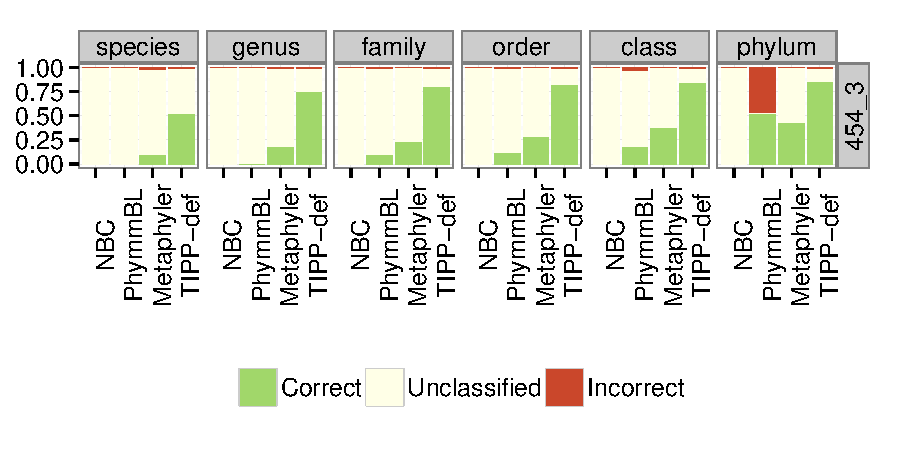
\includegraphics[scale=0.8]{tipp/higher_error_comparison_4_3_14.pdf}}
\end{center}
\caption{\label{tipp:comparison_methods} Non-leave-one-out experiments
          comparing the classification accuracy for NBC, PhymmBL, MetaPhyler
          and TIPP-default 
(i.e.,  TIPP-default refers to TIPP(95\%,95\%,100))
for fragments simulated from the 30 marker genes under different rates of 454-like errors.  Note that PhymmBL does not classify below the genus level and thus has 100\% unclassified rate at the species level.}
\end{figure}

PhymmBL performed reasonably well on the Illumina error-model conditions and the easier 454 error-model condition.  However, PhymmBL typically has more false classifications; this is most noticeable on the harder 454 model conditions.

While NBC had
excellent precision,  it had the worst recall of the methods.  
On the easiest Illumina model condition, NBC classified 
less than 60\% of the fragments at the phylum level.  
On the 454 model conditions, NBC's recall dropped by a considerable amount.  On the easiest 454 model condition, less than 20\% of the fragments could be classified at the phylum level.

MetaPhyler had very good performance on
Illumina error models, but poorer performance on the harder 454-error models.  For the Illumina error-model conditions,
MetaPhyler classified more than 90\% of the fragments correctly
at all taxonomic levels for the first two Illumina error-model conditions, but
dropped to 70\% or higher on the hardest Illumina error-model
condition.  On the 454 error-model condition, however, the percentage
of fragments
correctly classified by MetaPhyler rapidly dropped as the error rate
increases, with less than 50\% of the fragments classified correctly at
the phylum level on the hardest model condition.  

TIPP had very few incorrect
classifications for any error-model at any level.
 TIPP also had very good recall except
at the species level.
MetaPhyler had better recall at lower taxonomic ranks (species and genus)
with Illumina\_1 and Illumina\_2 error models. 

Not surprisingly, methods trained 
on the marker dataset vastly outperform
the composition-based methods on
sequences from these markers for taxon identification.
However,  
under the higher error models (especially
with 454 errors, which involve indels), we
see substantial differences between methods,
with TIPP showing high robustness to indels.  

One interesting question is whether taxonomic
classification methods can correctly identify
``dark matter" (sequences that do not belong
to known phyla  \cite{dark-matter}).
Since all fragments in my datasets come from known 
phyla, failure to classify these fragments
could be interpreted
as an assertion that the fragments belong to new phyla,
and so
would be a ``false positive" with respect to identifying
dark matter.
Figure 1 allows us to explore
this in a non-leave out experiment with 
indel errors under 454 models (low indel rates
for 454\_1 and higher rates for 454\_3).
Under low indel errors, 
TIPP and PhymmBL have generally low 
rates (less than 2\%) of incorrectly
identifying sequences as ``dark matter",
Metaphyler has slightly higher rate (6\%), and NBC
has an extremely high rate (72\%). 
Incorrect dark matter identification under
the 454\_3 error model is much higher:
100\% for NBC, 
56\% for  MetaPhyler, 
14\% for TIPP, and 2\% for PhymmBL.
These results show the challenges in interpreting failure to
classify sequences as indicative of membership in novel phyla,
especially for taxonomic identification  methods (such
as NBC and MetaPhyler) that 
attempt to minimize false positive identifications.
\paragraph{Summary.}
The taxonomic identification experiments showed 
interesting differences between TIPP, NBC, MetaPhyler, and PhymmBL.
On average TIPP had higher recall than MetaPhyler, 
with exceptions only on the non-leave-one-out 
experiments on the easier Illumina error models.  
On all other model conditions (454 non-leave-out experiments and all leave-out-experiments), TIPP had greater recall than MetaPhyler, with the largest improvement in recall at the lower taxonomic levels.  At the same time, TIPP also had lower precision in some (but not all) cases, but in most cases the reduction in precision was not as large as the improvement in recall. 
By design, 
NBC had very good precision, but
on these data
NBC also had
poorer recall  than the other methods.
PhymmBL was typically not as accurate as either MetaPhyler or 
TIPP (lower precision and recall), but was more accurate than NBC.

The experiments on abundance profiling
included MetaPhlAn and explored accuracy
with respect to RMSE. These experiments
showed somewhat different trends. 
On short fragment datasets,
TIPP and MetaPhlAn had better accuracy
than the other methods. TIPP and
MetaPhlAn
 had very similar
average accuracy, 
with
MetaPhlAn better on the MetaPhlAn datasets,
and TIPP generally better on the other datasets.
On long fragment datasets,
TIPP had generally
the best accuracy of all methods.
 PhymmBL was overall second best, and had the best
accuracy at the class level, 
and MetaPhlAn was in third place.

Since TIPP and MetaPhlAn are marker-based methods, and only
classify a fraction of the full set of fragments, this 
shows that good performance for abundance 
profiling does not rest on  the ability 
to classify all fragments, 
or even most fragments.
Instead, highly accurate classification of marker genes
can provide excellent estimations of taxonomic abundance.

More generally, 
abundance profiling can be improved by somewhat more
aggressive taxonomic profiling techniques, provided that
proportionally more correct than incorrect classifications result.
My comparison of the different TIPP variants suggest that the 
choice between which TIPP version to use depends on 
the context of the analysis; taxonomic identification analyses may benefit
by  minimizing false positive classifications by using TIPP(95\%,95\%,100), 
whereas abundance profiling analyses may 
benefit by using TIPP(0\%,0\%,100).  

\section{Conclusions and future work}\label{tipp:conclusion}
In this chapter, I presented TIPP, a new marker-based method for taxonomic identification and abundance profiling.  TIPP combines SEPP, a recent method for phylogenetic placement, with
statistical methods for evaluating the support for a given alignment and
phylogenetic placement, in order to give a highly accurate taxon
identification of each read.  Furthermore, by modifying
algorithmic parameters (such as the required statistical support), the user can
control for precision and recall, and depending on the context of the analysis, can optimize TIPP for taxonomic identification or for abundance profiling.

The SEPP technique of using multiple HMMs (instead of a single
HMM) is  part of the key to TIPP's improved 
accuracy as a taxonomic identification method, and suggests that
similar improvements for other methods that use single HMMs to 
perform classification 
might also be achievable. Therefore,
in my future work,
I plan to compare TIPP against mOTU \cite{Sunagawa2013}, a new marker-based profiling method that maps metagenomic reads to a reference dataset generated by HMMs, and to explore the impact on mOTU's performance by using SEPP's decomposition strategy in generating mOTU's reference dataset.

One important area of interest is the taxonomic identification of deeply branching phyla~\cite{dark-matter}.  The key step in detecting deeply branching phyla is searching for 
cellular organisms with very different 16S sequences.  Cells that have different enough 16S sequences are targeted for single cell sequencing.  TIPP can be used to aid in this endevour.  16S fragments can be selected from metagenomic samples and then classified using TIPP.  Since the focus is for searching on very divergent 16S sequences, the decomposition strategy used within TIPP may be helpful in obtaining more accurate classifications of the 16S fragments.  Samples that have high amounts of ``dark matter'' 16S fragments can then be targeted for single cell assembly.

% I explored TIPP's accuracy as a taxonomic identification method in comparison
% to several methods, with specific focus on how well it performed
% compared to MetaPhyler, which uses the same set of marker genes.
% These analyses showed that TIPP had
% substantially greater recall than MetaPhyler, while coming close to 
% (and in some cases improving on) the precision.  
% These improvements
% in classification accuracy explain why  TIPP produces
% more accurate abundance profiles than MetaPhyler.  
% 
% TIPP generally produced highly accurate
% abundance profiles.
% Although relative performance between methods changed 
% depending on the dataset, 
% on average, TIPP was as accurate or more so than the other methods I tested.
% TIPP had very good accuracy at the species level (a case where
% some methods do not make classifications, or make too few to do well
% at abundance profiles), and excellent accuracy at the other levels -
% for example, 
% TIPP had the best average accuracy at the phylum level of all methods we
% tested.
% The closest competition was with MetaPhlAn,
% another marker-based taxonomic identification method.
% These experiments show that marker-based profiling has
% the ability to provide highly accurate abundance profiles, even though
% only a fraction of the fragments are classified. 
% 
% The SEPP technique of using multiple HMMs (instead of a single
% HMM) is  part of the key to TIPP's improved 
% accuracy as a taxonomic identification method, and suggests that
% similar improvements for other methods that use single HMMs to 
% perform classification 
% might also be achievable. Therefore,
% in my future work,
% I plan to compare TIPP against mOTU \cite{Sunagawa2013}, a new marker-based profiling method that maps metagenomic reads
% to a reference dataset
% generated by HMMs, and to explore the impact on mOTU's performance
% by using SEPP's decomposition strategy in generating mOTU's reference dataset.
% 
% Finally, one of the main features
% of TIPP is the relative robustness to sequencing errors (both
% substitutions and indels), which I conjecture is due to the use of
% statistical techniques for multiple sequence 
% alignments to find good matches between the
% fragments and the reference alignment.
% Therefore, the high error rates commonly encountered in single-molecule
% sequencing technologies (up to 14\% insertion rate 
% for Pacific Biosciences technologies \cite{Carneiro2012})
% that are likely to be increasingly used in the context of metagenomic
% data may not be particularly
% problematic for TIPP.
% Instead, my results indicate that TIPP 
% may well continue to have good
% accuracy even as the quality of the data degrades.



\chapter{UPP: Ultra-large alignments using families of Hidden Markov Model}\label{upp_chapter}
\index{UPP@\emph{UPP}}%


In Chapter~\ref{sepp_chapter}, I showed that SEPP resulted in improved phylogenetic placement accuracy compared to HMMALIGN+pplacer and PaPaRa+pplacer.  In this chapter, I will show a modification to SEPP to allow large-scale alignment of a set of unaligned sequences.  This new technique, called UPP, allows accurate alignment of datasets containing both fragmentary and full-length sequences, is fast and highly parallelizable, and can generate an accurate alignment of up to 1,000,000 sequences.

Section \ref{upp:motivation} presents previous work on large-scale alignments.  In Section \ref{upp:algorithm}, I describe UPP, a modification of SEPP for ultra-large alignment.  In Section \ref{upp:evaluation}, I describe the simulation study designed to evaluate the alignment and phylogeny estimation accuracy of UPP on both simulated and biological datasets.  Section \ref{upp:results}, I present the results comparing UPP and other alignment techniques.  I show that UPP can be tuned for accuracy or speed, and that UPP generally results in better alignments than other methods, and that UPP is the only method can align the largest datasets in less than 24 hours on a 12 core machine.  Finally, in Section \ref{upp:conclusion}, I discuss future improvements to UPP, and ongoing studies using UPP.


\section{Motivation and previous studies}\label{upp:motivation}

Multiple sequence alignment (MSA), gene
tree estimation (which depends on an MSA), and species 
tree estimation (which can depend on the estimation
of multiple gene trees \cite{maddison,edwards})
are initial
steps in many bioinformatics pipelines, with applications to
orthology inference 
\cite{Afrasiabi2013},
biomolecular sequence structure and function prediction \cite{Eisen1998},
drug target identification \cite{Abadio2011},
and
the inference and quantification of selection
\cite{EisenFraser2003}.
Because of the impact of alignment estimation
error on these inferences 
\cite{WongSuchardHuelsenbeck2008,FletcherYang,JordanGoldman},
many methods have been developed to estimate
alignments \cite{DoKatoh,RussellMSAbook} and 
trees \cite{felsenstein_inferring_2003}.
Multiple sequence alignment of large datasets, containing
several thousand to many tens of thousands of sequences,
is sometimes necessary; examples include
% be useful for many applications, including
gene family tree estimation for multi-copy genes
(e.g., the p450 or 16S genes), viral evolution,
remote homology detection,
and the inference of deep evolution \cite{zwickl_increased_2002}; however, 
current MSA methods have poor accuracy on large
datasets, especially when they evolved under
high rates of evolution \cite{Liu2010}.
These limitations can discourage
biologists from utilizing the full range of biological data, and
affect downstream inferences.
I present UPP (Ultra-large alignments using Phylogeny-aware Profiles), 
a statistical MSA method that utilizes
a new machine learning technique -- the Family of Hidden Markov Models --
to address these limitations.
UPP is designed for multiple sequence
alignment estimation 
for single genes (including multi-copy genes
that can appear many times inside a single
organism), 
and produces  more accurate alignments on 
datasets that are large, that span large
evolutionary distances, 
or that contain fragmentary sequences.
UPP combines techniques designed for structural alignment prediction
and techniques designed for positional homology prediction
(two different
but related problems \cite{goldman-benchmark,Reeck1987}),
and provides excellent accuracy on both phylogenetic and
structural benchmarks. Furthermore, UPP is fast and very scalable,
producing alignments on 10,000 sequences in under an hour,
and on one million sequences in just over two days, using
a small number of processors.

UPP addresses the needs of current projects
that aim to construct alignments and trees on
large datasets, containing several hundred sequences or more.
Some of these projects are attempting to assemble
ultra-large trees, with many tens of thousands of sequences.
For example, 
iPTOL \cite{iptol} (the iPLANT Tree of Life 
project)
plans to construct a
tree on 500,000 plant species, and  
the Thousand Transcriptome Project \cite{1kp} is
constructing gene family trees with more
than 100,000 sequences for approximately 
1000 species.
Large-scale phylogenomic projects
like these
are enabled by next generation sequencing (NGS) technologies, 
which have made the generation of sequence data much
more affordable \cite{NGS}.
Upcoming sequencing technologies \cite{Mutz2013,KuRoukos2013}
will enable even 
larger datasets containing sequences from throughout
the genomes of many organisms.
Ambitious projects, such as the Genome 10K
Project \cite{Genome10k}, that plan to estimate
species trees with thousands to tens of thousands
of organisms, will be able to take advantage of
these new data, provided that computational methods
are available and able to provide sufficient accuracy
on ultra-large datasets.

Efficient maximum likelihood (ML) gene tree estimation for
datasets containing thousands \cite{Stamatakis2006} to tens of thousands
\cite{Price2010}  of
sequences is now feasible, but the accuracy of ML trees depends
on having accurate multiple sequence alignments \cite{Morrison2006}, and 
estimating highly accurate large-scale alignments 
is extremely challenging; indeed,
some datasets with only 1,000
sequences can be difficult to align well \cite{Liu2009,Liu2012}.
This is particularly true for non-coding data, which can 
evolve under higher rates of evolution than coding data,
making alignment estimation difficult
\cite{PrychitkoMoore2003}.
However, non-coding data can be essential
for species tree estimations of rapid radiations;
for example, the avian phylogenomics project
%estimated an avian phylogeny for 48
%species and approximately 14,000 markers
%and
observed that intron alignments provided
substantially higher levels of phylogenetic
signal than exon alignments for estimating
the avian phylogeny \cite{StatisticalBinning,jarvis2014}.


MSA methods have also been evaluated with respect
to accuracy defined by shared structural features in proteins, and
one approach for estimating alignments uses
 ``templates", which
are statistical models of the molecule (often Hidden Markov Models \cite{Eddy1998}).
Although template-based MSA methods 
(e.g., 
\cite{neuwald2009,Nawrocki2009,ShangGardnerGutell,satchmo03,kimmen2010,promals,clustal-omega})
often perform well under
structural alignment criteria,
 it is not clear
how well they will perform when
phylogenetic estimation is the objective \cite{Morrison01022009,goldman-benchmark}.
On the other hand, multiple sequence alignment
methods designed for phylogenetic estimation 
(e.g., % Prank \cite{Loytynoja2005}  and 
BAli-Phy \cite{rs06,rs07})
tend to be 
limited to datasets that are small and have low rates of evolution.
More generally, studies show that 
phylogenetic estimation accuracy is typically reduced
when alignments are estimated on large datasets
that evolve under high rates of evolution
\cite{Liu2009,liu-ploscurrents}.
SAT\'e-I \cite{Liu2009} and SAT\'e-II \cite{Liu2012} 
%and PASTA \cite{pasta} were
co-estimate gene sequence alignments and 
trees, and have better accuracy and scalability than standard
multiple sequence alignment methods for large
datasets; however, even SAT\'e-II (which improves
on SAT\'e-I) 
is limited to datasets with at most 50,000 sequences.
PASTA \cite{PASTA} is the most recent
addition to the SAT\'e suite of methods, and
can analyze datasets with up to 200,000 sequences.
However, SAT\'e-I, SAT\'e-II, and PASTA have not
been evaluated for structural
alignment purposes, nor as protein alignment methods.


\begin{figure}[htpb]
\centering
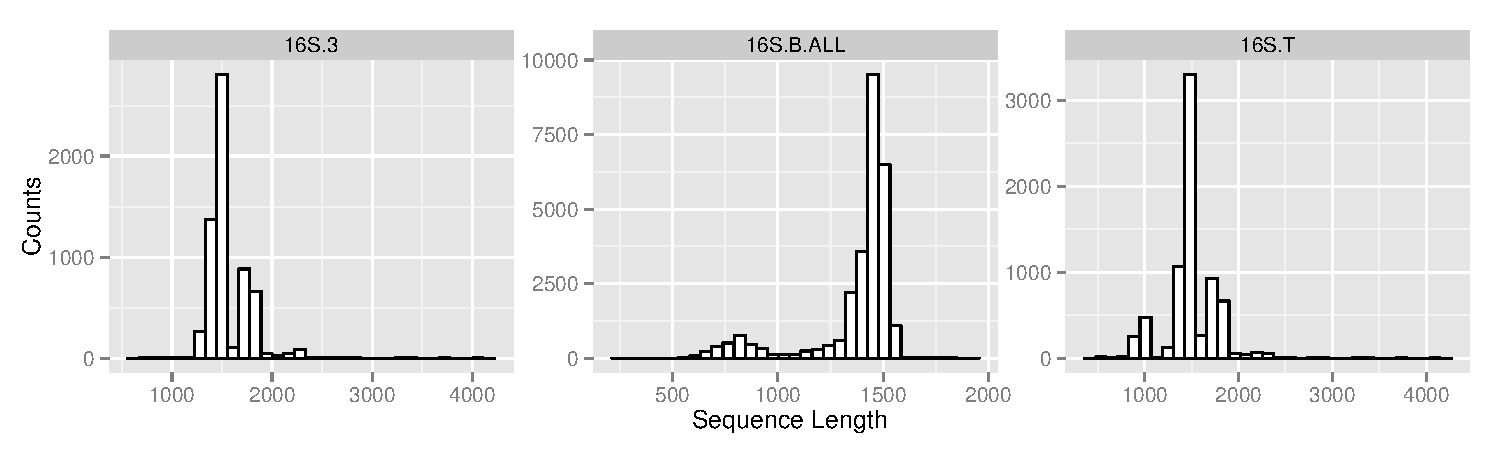
\includegraphics[width=1.0\linewidth]{{upp/length.gutell.1.30}.pdf}\\
\caption[Histogram of sequence lengths for the 16S Gutell CRW datasets.]{\label{gutell_length}  {\bf Histogram of
sequence lengths for the 16S Gutell CRW datasets.}  The histogram
of sequence lengths for the three CRW datasets demonstrates
substantial sequence length heterogeneity, especially
for 16S.T.
%a histogram of sequence lengths for 16S from the Gutell CRW datasets.  
The average length of the 16S sequence is approximately 1500.}
\end{figure}


\begin{figure}[htpb]
\centering
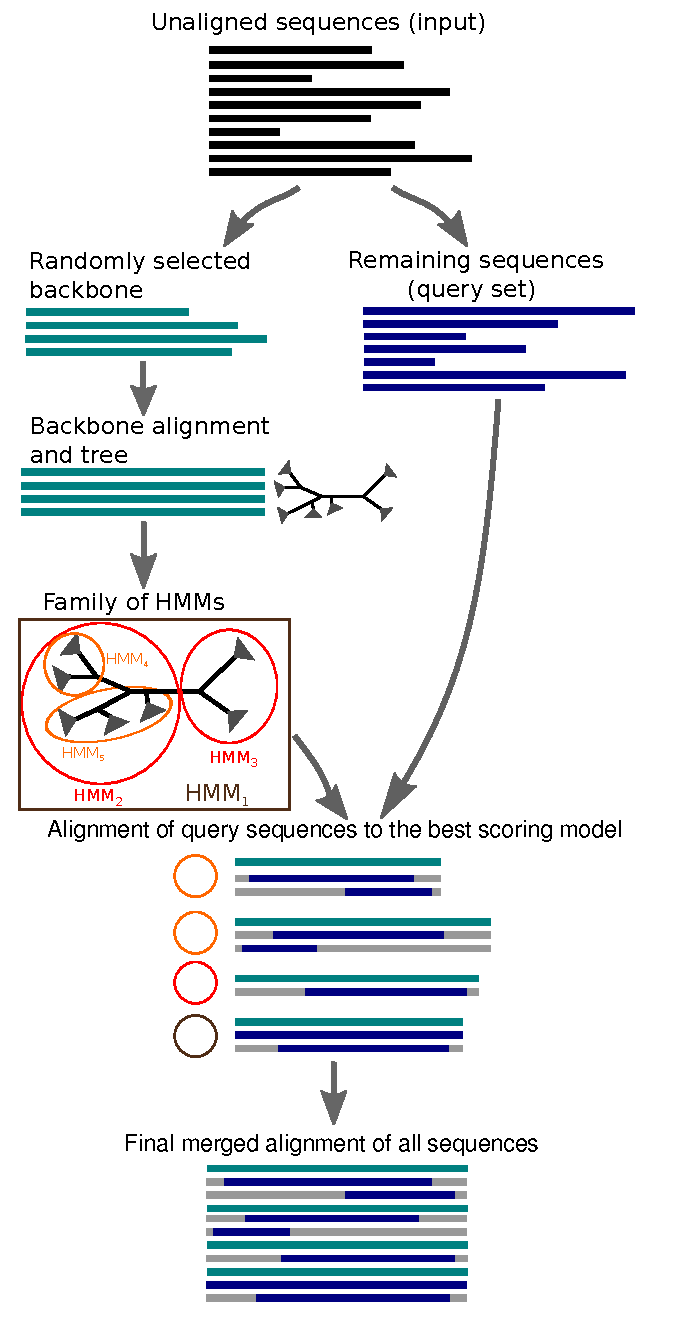
\includegraphics[width=.65\linewidth]{upp/diagram}  
\caption[Overview of the UPP algorithm.]{\label{flow_chart}  
{\bf The UPP algorithm and the HMM Family technique.}}
\end{figure}

Furthermore, many biological datasets contain
substantial numbers of 
fragmentary sequences 
(Fig.~\ref{gutell_length} and figs.~\ref{homfam_length}
and \ref{balibase_length} in the
supplementary online materials \cite{SOM}),
resulting in part from incomplete assembly or
insufficient transcript sampling.  % \cite{why-fragments}.
Although some methods (e.g., HMMER \cite{Eddy1998,HMMER} and MAFFT-Profile \cite{Katoh2012})
can add individual sequences (even short fragments) into existing alignments,
MSA methods are not designed to analyze datasets containing
a mixture of fragmentary and full-length sequences, and
have not been
tested under these conditions.
Thus, little is known about the accuracy of 
alignments on datasets of any size that contain
fragmentary sequences, nor about the accuracy of
trees estimated on such alignments.

Thus, large-scale multiple sequence alignment estimation is
a basic step in many problems, including gene tree estimation and
protein structure and function prediction, but
existing methods have not been shown to provide sufficient accuracy
on datasets that are large, that evolve under high rates of evolution,
or that contain fragmentary data. 
The new technique I present, UPP, addresses these challenges.

\section{UPP: Ultra-large alignment using Phylogeny-aware Profiles}\label{upp:algorithm}
UPP begins with unaligned sequences, and selects a subset
(called the ``backbone dataset") of the sequences,
and the remaining sequences are the ``query sequences".
 %, restricted to those that
UPP preferentially selects the backbone
sequences from  those that are considered to be ``full-length", in order to
provide robustness to fragmentary data.
UPP uses PASTA to compute an alignment and a tree on the backbone sequences
(called the ``backbone alignment" and ``backbone tree", respectively).
The backbone tree is then used to create a collection of subsets of the sequence dataset,
with subsets ranging in size from at most ten to up to the full dataset,
and all but the smallest subsets contain other subsets
(see Fig.~1, Methods, and Section \ref{upp_alg} for additional details).
UPP adds each
query sequence into the backbone alignment
using methods (HMMBUILD, HMMSEARCH,
and HMMALIGN) within the HMMER  suite of
tools, as follows. First, UPP uses HMMBUILD to build profile HMMs, one
for each subset alignment (defined to be the backbone
alignment restricted to the subset sequences); this is
called the ``HMM Family".
The fit of each query sequence
to each HMM is then assessed using HMMSEARCH; this 
returns a ``bit score", which is
a measure of the quality of the match between
the query sequence and the HMM. 
The subset HMM with the best bit score is selected, and the 
sequence is added to the subset alignment using HMMALIGN.
By transitivity, this process defines how the query sequence should
be added into the backbone
alignment. Once all the query sequences are added
into the backbone alignment, transitivity defines the final
output multiple sequence alignment. 

UPP can also be used iteratively. In the
first iteration, the UPP alignment is computed,
and a ML tree is estimated using
FastTree.
This ML tree is then used to select the backbone dataset
for the next iteration, thus ensuring
appropriate phylogenetic diversity in the backbone.
While this resampling technique is generally beneficial,
it is particularly helpful
where there is highly uneven taxon sampling (e.g., a densely sampled
in-group and very sparsely sampled distant outgroup), 
when %However, resampling is also helpful when
 fragmentary sequences are unevenly distributed throughout the
phylogeny, or when sequence lengths changed substantially
over evolutionary history.
In each of these cases, 
the technique used to select backbone sequences could
lead to backbones that fail to have
adequate representation in all the major clades -- thus reducing
the accuracy of the resultant alignment.

\paragraph{The UPP algorithm.}
I describe a single iteration of UPP run
in default mode;
see Section \ref{upp_alg} for additional details.
The input to UPP is a set of sequences.
In the first step, UPP determines whether the
dataset has fragmentary sequences, based
on the estimated median length 
of ``full-length" sequences.
Any sequence that is shorter than 75\% of this
median length,  or longer 
than 125\% of the median length, is
not considered to be full-length, and will not be 
included in the backbone dataset (except
in a ``directed sampling" step, as described
earlier).
Then, a random subset $S_0$ of 1000 full-length  sequences
is selected,
%sequences that are considered to be ``full-length"
%(defined to be with 75\% and 125\% of the known or estimated median length
%of full-length sequences for the molecule)
 and a PASTA alignment $A$ and tree $T$ are
computed on the subset.
(If the number of full-length sequences is less than 1000,
then $S_0$ is the entire set of full-length sequences.)
The set $S_0$ is called the ``backbone dataset" and
the tree and alignment computed using PASTA on 
$S_0$ are called the ``backbone alignment" and
``backbone tree".

The backbone tree is then used to produce a
collection $\mathcal C$ of subsets of the backbone
dataset, as follows.
First, $\mathcal C$ is initialized
to include $S_0$.
Then an edge in the backbone tree $T$ is found
whose removal splits the tree into two 
subtrees of approximately equal size;
this edge is called a ``centroid edge",
and the leaf sets of the two subtrees produced by removing
the centroid edge  are added to $\mathcal C$. 
At this point, $\mathcal C$ contains three sets: one
containing the entire set of backbone sequences, and two others
with roughly half the backbone sequences.
This  process is repeated on every subtree with more
than ten leaves.
Thus, the collection $\mathcal C$ contains a set of
subsets of $S_0$, where the smallest subsets might
contain fewer than ten leaves, and where every subset
(except for  the
smallest subsets) contains two other subsets.
For example, if the backbone tree contains 1000 leaves, then
$\mathcal C$ would contain one set of
$1000$ sequences, two sets of approximately $500$ sequences, four sets of
approximately $250$ sequences, etc., 
down to some number of sets
with ten or fewer sequences.

I then compute the backbone
alignment restricted to each subset of sequences in $\mathcal C$;
%omitting the sites that are fully gapped within each subset
%alignment; 
these are called the subset alignments.
I use HMMBUILD (from the HMMER3 suite of tools)
to build an HMM on each subset alignment,
with a match state for each site that has at least one
non-gap character (note that this is not the default
way of running HMMBUILD). 
This produces a set $\mathcal{H}$ of profile HMMs,
one for every subset alignment, with approximately the
same number of states in each HMM (the only
condition where different profile HMMs will have 
different numbers of states are when the subset alignments
contain different numbers of all-gap sites).

Each sequence in $S-S_0$ is called a query sequence.
I use HMMSEARCH (which takes alignment
uncertainty into account)
to compute the fit between each
query sequence and each profile HMM in $\mathcal{H}$.
%, using the local alignment command. %Nam?
%HMMER 3 is only local alignment no global alignment so not
%necessary to point this out
The HMM with the best fit (defined by the
best bit score returned by HMMSEARCH) is
selected for the query sequence.

HMMALIGN is then used to add  
query sequence $s$ to the
subset alignment $A_s$
associated to the HMM $H_s$ selected by $s$.
This produces a local alignment of $s$ to $A_s$ 
(and hence an alignment of $A_s \cup \{s\}$). 
By transitivity, 
this defines how to add $s$ into the  backbone alignment on $S_0$,
which I call the ``extended alignment for $s$".
When the sequence $s$ has 
a character  (nucleotide or amino acid)
that is not aligned to anything in the backbone
alignment, the extended alignment will have
an ``insertion site".
%that contains only one letter, contributed by query sequence $s$.


Once all the extended alignments are computed, I can merge
them all into a single multiple sequence alignment on $S$.
This approach will tend to have potentially many insertion sites,
%each produced by a single query sequence,
which  can be 
masked out during the tree estimation step to improve
speed.

UPP can be used iteratively,
but iteration only occurs if the distribution of
backbone sequences in a tree estimated on the UPP alignment
provides inadequate phylogenetic diversity.
Thus, the first step is to determine if 
all the major clades in  the estimated tree
contain at least one tenth of the
expected number of backbone sequences.
If the estimated tree passes this test, no resampling is triggered.
Otherwise, UPP uses the tree to select the backbone
sequences, ensuring that every major clade contributes
appropriately to the backbone sequence dataset.
See 
Sections \ref{commands}, \ref{hmm_commands}, and \ref{upp_alg}
for additional details.


\section{Performance evaluation}\label{upp:evaluation}
I demonstrate UPP's accuracy on a collection of biological
and simulated datasets, in comparison to leading multiple
sequence alignments. 
I compare estimated alignments 
to reference (true or curated) alignments, 
and ML trees on these alignments to 
reference trees, and record alignment error and tree error.
%Our study shows that UPP typically produces more
%accurate alignments than  the leading MSA methods for large-scale 
%multiple sequence alignment of both nucleotide and
%amino acid datasets, especially for datasets in the ``twilight zone" where
%high evolutionary distances make sequence homology 
%hard to distinguish from chance similarity.
%UPP is highly robust to fragmentary datasets,
%and fast enough to run on very large 
%datasets -- even up to one million sequences -- using 
%a small number of processors.
%Furthermore, 
%maximum likelihood (ML) trees based on UPP 
%alignments are typically 
%more accurate than ML trees based on other alignments.
%Thus, highly accurate \emph{de novo} ultra-largescale 
%multiple sequence alignment and
%tree estimation is achievable, even without supercomputers.

\paragraph{Datasets.} 
Because structural alignment and phylogenetic alignment
have different purposes and potentially different
criteria \cite{Reeck1987,goldman-benchmark}, I use both simulated and biological datasets (with structurally-based
alignments) to evaluate UPP in comparison to other MSA methods.


The simulated datasets include 1000-sequence nucleotide datasets 
with average length 1000-1023 
from \cite{Liu2009} that were
generated using ROSE \cite{ROSE}, and
used to evaluate SAT\'e in comparison
to other MSA methods on large datasets;  10,000-sequence datasets we
generated using Indelible v.~1.03 \cite{Fletcher01082009} with average
sequence length 1000;
and subsets of the million-sequence RNASim \cite{RNASim} dataset
with average sequence length 1554.5.
RNASim is a simulator for RNA sequence evolution
that I present here, 
and that was designed to simulate a complex molecular evolution process using
a non-parametric population genetic model that generates long-range statistical dependence
and heterogeneous rates.
%Tandy - write something
The simulated AA datasets include the  5000-sequence datasets 
from \cite{Price2010}, which were
generated using ROSE based
on proteins from the COG database \cite{COG},  and had
average sequence lengths
varying from 179.4 to 346.9.


The biological datasets include the three largest 
datasets from the
Comparative Ribosomal Website (CRW)  \cite{Cannone2002}, each
a set of 16S sequences. I include
the 16S.3 dataset (6,323 sequences of average length 1557,  spanning three phylogenetic domains), the 
16S.T dataset (7,350 sequences of average length 1492,  spanning three phylogenetic domains), 
and the 
16S.B.ALL dataset (27,643 sequences of average length 1371.9,  spanning the bacteria domain).  
The CRW datasets have highly reliable, curated alignments inferred 
from secondary and tertiary structures.  
I include ten 
large amino acid
datasets (10 AA) with curated multiple sequence alignments (the eight 
largest
BAliBASE datasets \cite{Thompson2011}
and IGADBL\_100 and coli\_epi\_100 from \cite{Gloor2005}); these
range in 
size from
 320 to 807 sequences and have average
sequence lengths that range from 56.7 to 886.3.
I also used 19 of the largest HomFam datasets, which are amino acid 
sequence datasets ranging in size from 
10,099 to 93,681 sequences,  and
having average sequence lengths ranging
from 29.1 to 469.8;
these datasets 
were used in \cite{Sievers2011} to evaluate protein multiple
sequence alignment methods on large datasets, and have
Homstrad \cite{homstrad} reference alignments
on very small subsets (5-20 sequences, median 7) of their sequences.
%Tandy - put in range of the reference alignment sizes

I generated fragmentary datasets by selecting 
a random subset of sequences and a random substring (of a desired
length) for each selected sequence (see 
Section \ref{frag_simulation} for full details).
Empirical statistics (number of sequences, number of sites in the reference alignment,
average and maximum p-distances, average
gap length, and percent of the matrix that is gapped) for each dataset 
and  model condition
can be found in Tables \ref{empirical_stats_simulated} and \ref{empirical_biological}.

\paragraph{Reference alignments and trees. }
For simulated datasets, the reference
alignment is the true alignment (known because
I simulate evolution and record the events); for
biological datasets, the reference alignment is the
curated structural alignment.
Reference trees for the simulated datasts are
the model trees that
generate the data.  For the biological datasets, we
use RAxML with bootstrapping on the reference alignments to
obtain ML 
trees with branch support,
and then I collapse all   branches with less than
75\% support;  this is the
same technique used in \cite{Liu2012} to
produce the reference trees on the CRW datasets.
The reference trees for the biological datasets 
are typically incompletely resolved.
In this case,  
the recovery of low support branches in the biological datasets is largely influenced by chance,  making
the FN rate preferable to the
standard bipartition error rate, also called the
Robinson-Foulds (RF) \cite{RF} error rate.
FN rates are identical to the RF
error rates when 
estimated and reference trees are fully resolved, and so
FN rates are also appropriate
for the simulated dataset analyses; 
hence, I report FN rates for all analyses, using
\cite{fasttree_tools}.

\paragraph{Fragment Simulation}\label{frag_simulation}

In order to test the robustness of different alignment methods to
fragmentary sequences, I generated datasets with both full-length and fragmentary sequences from the 1000-taxon 1000M2, 1000M3, and 1000M4 datasets, the CRW datasets, the Indelible datasets, and the RNASim 10K dataset.  For each dataset, a fraction of the sequences (12.5\%, 25\%, or 50\%) were made fragmentary by selecting a contiguous substring (length drawn from a normal distribution with mean length of 500 bps and standard deviation of 60 bps) from a random position (drawn uniformly, at random) from the original full-length sequence.  The remaining sequences that were selected to be full-length were left unmodified.

For each of the 1000-taxon fragmentary datasets, 5 replicates were generated.  For the larger CRW, Indelible, and RNASim 10K datasets, only 1 replicate was generated.
\clearpage

\paragraph{Methods. }
I use 
Clustal-Omega \cite{Sievers2011} version 2.1, 
MAFFT \cite{Katoh2005,Katoh2007} version 6.956b,
%Mafft-L-INS-i~\cite{Katoh2002,Katoh2005}, 
%Mafft-PartTree \cite{Katoh2007}, 
%MAFFT-Profile \cite{Katoh2012}, 
Muscle \cite{Edgar2004} version 3.8.31, 
Opal \cite{Wheeler2007}, %version number, Nam?
PASTA, %version number, Nam?
SAT\'e-II \cite{Liu2012}, %version number, Nam?
and UPP to compute multiple sequence alignments.
%The UPP analysis of the 16S.T dataset triggered a
%second iteration (due to uneven taxonomic distribution of fragments);
I show results for only
iteration of UPP in the main paper; see Section \ref{resample_16S}
for results using more than one iteration.
%MAFFT-Profile. 
I use FastTree \cite{Price2010} and RAxML \cite{Stamatakis2014} 
to compute maximum
likelihood trees on estimated and reference alignments.



\paragraph{Performance Metrics.}
I compare estimated alignments and their maximum
likelihood (ML) trees to reference 
alignments and trees.
I use FastSP \cite{fastsp} to 
compute
alignment error, recording
 the sum-of-pairs false 
negative (SPFN) rate (which is the percentage of the
homologous pairs in the reference alignment that
are not in the estimated alignment) and the
sum-of-pairs false positive (SPFP) rate
(which is the
percentage of homologous 
pairs in the estimated alignment that are not present in the reference alignment).
SPFN and SPFP rates are given in the SOM, and the means
of these two
alignment error rates are given in the main paper.
I report tree error using the false negative (FN) rate (also
known as the missing branch rate), which is 
the percentage of internal edges in the reference tree that 
are missing in the estimated tree.
I also report $\Delta{FN}$, the difference between 
the FN rate of the estimated tree versus the FN 
rate of the tree estimated on the true alignment, to 
evaluate the impact of alignment estimation error on
phylogenetic analysis.
Most typically, $\Delta(FN)>0$, indicating that the estimated tree
has higher error than the ML tree on the true alignment.



\paragraph{Computational resources. }
The majority of experiments were run on the
homogeneous Lonestar  cluster at
the Texas Advanced Computing Center (TACC).
Because of limitations imposed by TACC, these
analyses are limited to 24 hours, using
 12 cores with 24 GB of memory;
methods that failed to complete within 24 hours or 
terminated with an insufficient memory error message were marked as failures.  
For experiments on the million-sequence RNASim dataset,
I ran the methods on a 
dedicated machine with 250 GB of main 
memory and 12 cores and ran until an alignment 
was generated or the method failed.  
I also performed a limited number of experiments on TACC with
checkpointing, to explore performance 
when time is not limited.  


\section{Results}\label{upp:results}
\paragraph{Initial experiments. }
I let UPP(Default) denote the default version of UPP
in which I use
backbones of 1000 sequences, use PASTA to compute
the backbone alignment, and add sequences to  the backbone
alignment using
the HMM Family technique.
I also explore UPP(Fast), the variant
where I use   use backbones of 100 sequences but keep the
other algorithmic parameters fixed, and ``NoDecomp"
versions of UPP(Fast) and UPP(Default)
to indicate that
I use just one HMM instead of a family of HMMs
to represent the backbone alignment.
I show results for one iteration of UPP.


Since UPP computes its backbone using PASTA,
I compared UPP to PASTA, and included
a comparison to SAT\'e-II, focusing on
the RNASim datasets. % (Section \ref{sec:som-upp-vs-pasta}).
As shown in  \cite{PASTA},
PASTA is
more accurate than SAT\'e-II, can analyze larger datasets,
and is computationally more efficient than SAT\'e-II.
A comparison between UPP(Default), SAT\'e-II, and PASTA shows that 
UPP(Default) typically had the lowest
alignment error rates
(figs.~\ref{rnasim_pasta_alignment}-\ref{homfam_pasta_alignment})
and was much more robust to fragmentation
(fig.~\ref{frag_1000M2_pasta_alignment}). 
UPP produced more accurate trees than SAT\'e-II 
(fig.~\ref{rnasim_pasta_tree}).
PASTA had a small advantage over UPP with respect to tree estimation
on datasets without fragments
(fig.~\ref{rnasim_pasta_tree}), but was less accurate
than UPP on datasets with fragments
(fig.~\ref{frag_1000M2_pasta_tree}).
%Nam - verify that the 16S.T figure is using UPP with two iterations
UPP(Fast) was  also able to analyze larger datasets 
than PASTA and SAT\'e-II:  the  million-sequence RNASim dataset
was analyzed by UPP(Fast, NoDecomp) in 52 hours, but
PASTA failed to complete on the dataset and SAT\'e-II failed to
complete on even the 100K RNASim dataset (section \ref{early_termination}).
I focus the remainder of the discussion on Clustal-Omega, Muscle, 
MAFFT, and UPP;
results for the full set of methods can be found in Section 
\ref{sec:all_methods}.  

\subsection{Phylogenetic alignment accuracy}
I begin by evaluating UPP for phylogenetic estimation purposes.
I use simulated datasets, since these provide
true alignments and true trees, and thus allow us
to exactly quantify error in identifying true positional homology
(i.e., descent from a common ancestor \cite{Reeck1987}).

\begin{figure}[htpb]
\begin{subfigure}[htpb]{\textwidth}
  \centering
  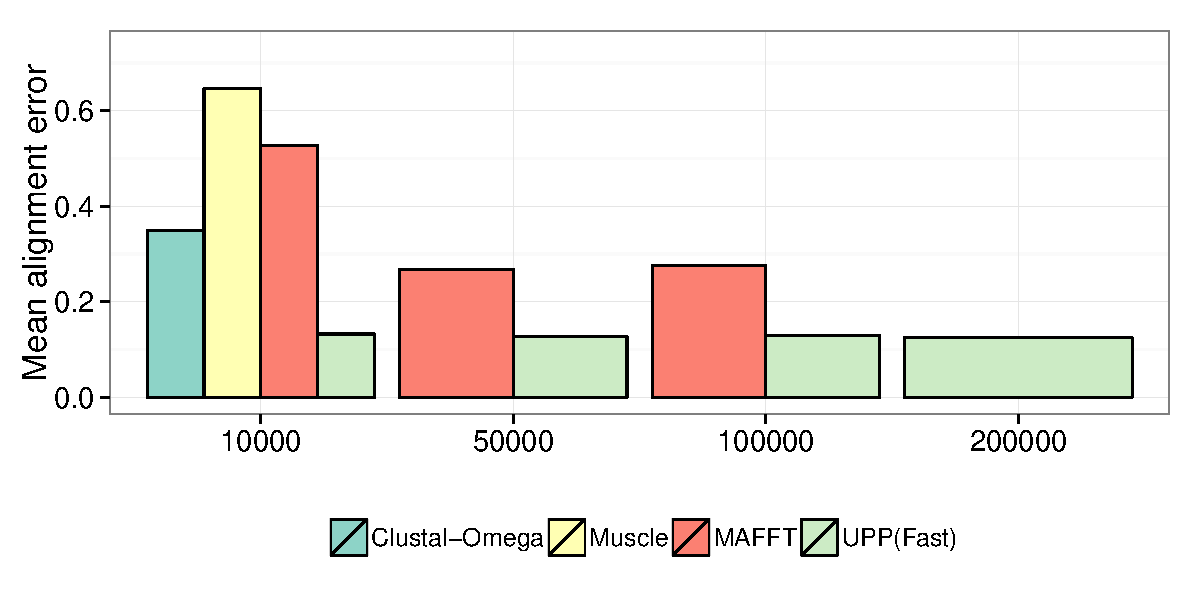
\includegraphics[width=0.60\linewidth]{{upp/rnasim.main.alignment_average}.pdf}\\
  \caption[]{Alignment error on RNASim datasets with 10K to 200K sequences}
\end{subfigure}
\begin{subfigure}[htpb]{\textwidth}
  \centering
  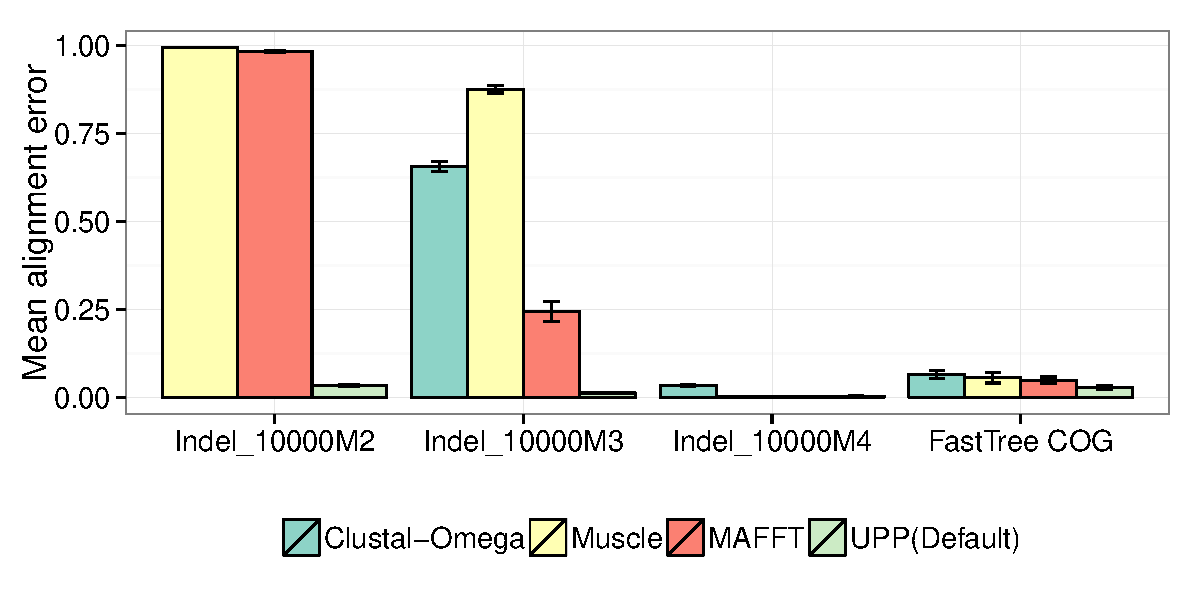
\includegraphics[width=0.60\linewidth]{{upp/all_simulated.main.alignment_average}.pdf}\\  
  \caption[]{Alignment error on other simulated datasets}
\end{subfigure}  
\begin{subfigure}[htpb]{\textwidth}
  \centering
  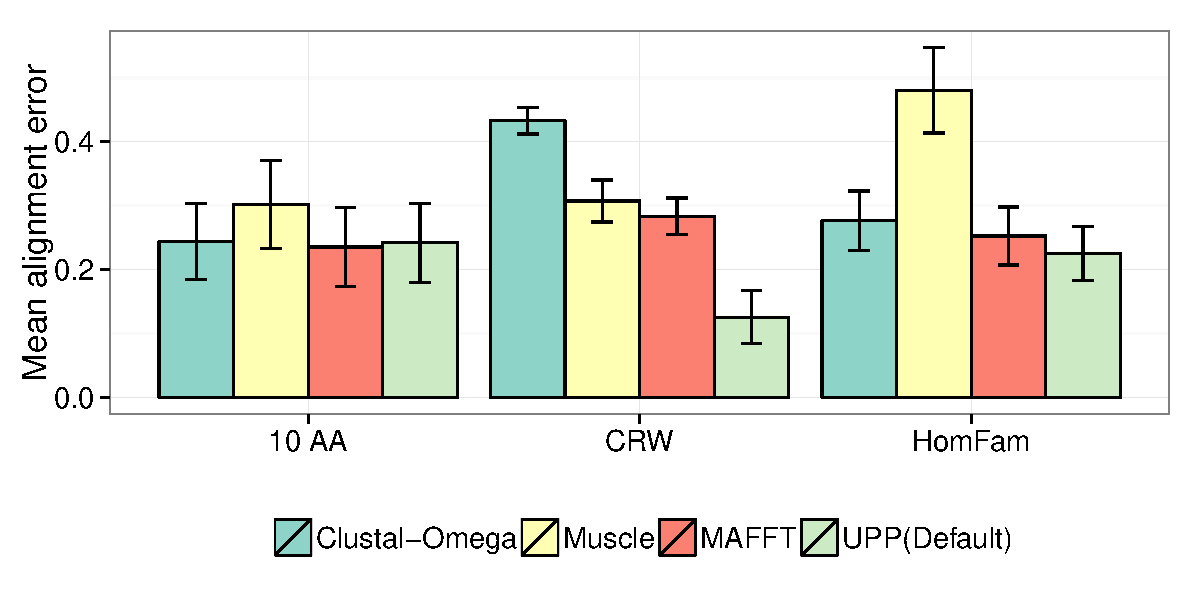
\includegraphics[width=0.60\linewidth]{{upp/all_biological.main.alignment_average}.pdf}\\  
  \caption[]{Alignment error on biological datasets}
\end{subfigure}  
\caption[Alignment error rates on different datasets.]
{\label{align_error}  {\bf Alignment error rates on 
simulated and biological datasets. }  
All methods were 
run with 24 GB of memory and 12 CPUs, and given 24 hours to complete.  
MAFFT is run using L-INS-i on the 10 large AA datasets, using default MAFFT on the FastTree COG datasets, HomFam datasets, and the CRW 16S.T and 16S.3 datasets, and using 
the PartTree command
for the CRW 16S.B.ALL dataset (default MAFFT failed to align this dataset).
Results not shown are due to methods failing to return an alignment
within the 24 hour time period on TACC, using 12 processors.
% Muscle fails to run on datasets with 50K sequences or more due to insufficient memory.  Similiarly, MAFFT-profile(Fast) fails on the 200K dataset due to insufficient memory.  Clustal-Omega fails to generate an alignment within the 24 hour time limit on datasets with 50K sequences or more.  
}  
\end{figure}


\paragraph{Alignment estimation error on RNASim datasets. }
I examined performance on the RNASim datasets with
up to 200,000 sequences, using
UPP(Fast) to
reduce running times
(results obtained using backbones of 1000
sequences showed improved accuracy but took longer; 
see Table~\ref{table:rnasim_upp_variants}).
I compare UPP(Fast) to MAFFT (default MAFFT on the 10K and 50K datasets, MAFFT-PartTree on 100K dataset),
Clustal-Omega, and Muscle (Fig.~\ref{align_error}(a)). 
Default MAFFT produced less accurate alignments %but more 
%accurate trees 
than MAFFT-PartTree on the RNASim 10K dataset (fig.~\ref{mafft_default_parttree})
and failed to complete on the 100K and larger datasets (Section
\ref{early_termination}).
%UPDATE with new results for baldr tree

UPP(Fast) succeeded in analyzing all the 
datasets within the 24 hour time limit, MAFFT-PartTree succeeded in analyzing the
datasets with up to 100K sequences, and default MAFFT successfully analyzed datasets with up to 50K sequences; however,
the other methods failed to align RNASim datasets with more than
10K sequences.
Muscle failed because it
required more than 24 GB of memory on these larger datasets, 
and Clustal-Omega 
failed to return an alignment  but
without giving an error message (see Section \ref{early_termination}
for details). % (see SOM for details).
%Nam, please check this
%This will need to be updated, looks like Mafft-PartTree might
%not have memory problem up to 100K (didn't terminate early like
%previous runs, still running.  Maybe be due to using latest version of Mafft
%Still segfaults on 200K with error message.  Will update SOM when runs complete
%/work/01722/namphuon/bin/mafft: line 2028: 10329 Segmentation fault      "$prefix/splittb fast" $legacygapopt -Z $algopt $splitopt $partorderopt $parttreeoutopt $memopt $seqtype $ model -f "-"$gop -Q $spfactor -h $aof -p $partsize -s $groupsize $treealg -i infile > pre 2>> "$progressfile"
On the RNASim 10K dataset
(Fig.~\ref{align_error}(a)), the error rates were
13.3\% for UPP(Fast),  
34.9\% for Clustal-Omega, 52.7\% for default MAFFT,
%Nam: changed MAFFT result to MAFFT-default, March 16
and 64.6\% for Muscle. 
UPP(Fast)'s 
alignment error rate was quite stable across all
numbers of sequences (up to 200,000), varying between 12.5-13.3\%.


I analyzed the million-sequence
RNASim dataset using UPP(Fast), UPP(Fast,NoDecomp),
and UPP(Default,NoDecomp),  
using  a dedicated machine, allowing the analysis to
exceed the 24 hour time limit in TACC.  
Both UPP(Fast, NoDecomp) and UPP(Default, NoDecomp) completed in less than three days 
and produced very accurate alignments %(52 versus 65 hours and 
(13.0\% and 11.1\% alignment error, respectively; see
Table \ref{alignment_large}).  
UPP(Fast) took 12 days to
align this dataset, and  produced a slightly more accurate alignment than UPP(Fast, NoDecomp) (alignment error 12.8\%).

\paragraph{Results on the Indelible NT simulated datasets. }
The 10,000-sequence Indelible simulated datasets evolved under 
low (10000M4), moderate (10000M3), or high 
(10000M2) 
rates of evolution. 
The difficulty in estimating alignments increased with the
rate of evolution; therefore,
I refer to these model conditions
as easy (10000M4), medium (10000M3), and hard (10000M2).
I ran UPP(Default), 
MAFFT-Default,
%Nam, perhaps Default MAFFT
%Still running
Muscle, and Clustal-Omega on ten replicates
for each model condition. 

UPP had very low average alignment error across 
all three model conditions:
3.3\%, 1.3\%, and 0.1\% on
the hard, medium, and easy 
% average alignment error on the hardest model condition, and 
%1.3\% and 0.1\% average alignment error on the medium and easy 
model conditions, respectively
(Fig.~\ref{align_error}(b)).
The accuracy of the other methods, however,
degraded rapidly with the increase
in the rate of evolution.   
For example, under the hard model condition,
Muscle had 99.5\% average alignment error,
MAFFT-Default had 97.9\% error 
and Clustal-Omega failed to generate an alignment
(Fig.~\ref{align_error}(b)).
Under the medium model condition,  
MAFFT-Default had 22.8\% error,  %Nam
 Clustal-Omega had 65.6\% error, %Nam?
and Muscle had 87.6\% error (Fig.~\ref{align_error}(b)). %Nam
%Nam: Numbers have all been corrected
%Nam: updated MAFFT-Default alignment March 16th
Finally, under the easy model condition,
MAFFT-Default, Muscle and UPP all had very low error (below 0.4\%),
and
Clustal-Omega had 3.4\% error (Fig.~\ref{align_error}(b) and
figs.~\ref{indelible_main_alignment} and \ref{indelible_spfn_spfp_alignment}).

\paragraph{Results on simulated AA datasets with 5000 sequences. }
%Nam - put in correct numbers - the ones that were here
%don't match the figures, so I am eyeballing them
%Nam: done
On the 5000-sequence simulated amino acid datasets,
UPP had very low error (2.9\%),
MAFFT-Default had 4.9\%, 
Muscle had 5.5\%,
and Clustal-Omega had 6.5\% (Fig.~\ref{align_error}(b),
figs.~\ref{fasttree_main_alignment_average}-\ref{fasttree_spfn_spfp_alignment}).

\paragraph{Results on 1000-sequence simulated 
nucleotide datasets. }
The nine 1000-sequence model  
conditions 
studied in \cite{Liu2009,Liu2012} varied in
gap length distribution
 and overall difficulty
(as influenced by the relative
frequency of insertions and deletions (indels) to substitutions, and rate of evolution).
Although there is sequence length heterogeneity in
these  datasets, all sequences fall within the
range considered ``full-length"; therefore, because
these datasets have only 1000 sequences,
UPP(Default) is identical to PASTA on these data.
I were able to
run    Opal and MAFFT-L-INS-i (the most accurate
version of MAFFT)
in addition to Clustal-Omega, Muscle, 
and UPP(Default).  
%see Figures
%\ref{1000_taxon_main_alignment}  and \ref{1000_taxon_main_spfn_spfp}.
Error rates varied across the model
conditions, 
but the relative performance of methods
was fairly stable:
UPP(Default) and Opal had the lowest
alignment error rates (with UPP(Default)
more accurate than Opal under 
all models except those with the lowest
rate of evolution), 
Muscle and MAFFT-L-INS-i were typically
close in error (with  about twice 
as much error as UPP(Default) and Opal),
and Clustal-Omega had the highest error
(fig.~\ref{1000_taxon_main_alignment}).
As an example, on 1000M3, one of the easiest model conditions,
UPP(Default) and Opal had
the lowest alignment errors (5.6\% and 5.4\%,
difference not statistically significant),  %Nam - please calculate
followed by MAFFT-L-INS-i (14.1\%), Muscle (15.1\%),
and finally Clustal-Omega (34.3\%).
On 1000M1, one of the hardest model conditions,
UPP(Default) had  19.9\% error, followed 
by Opal with 25.1\%, MAFFT-L-INS-i with 52.2\%,
Muscle with 52.5\%, 
and finally by Clustal-Omega with 91.8\%.
%Figure \ref{1000_taxon_main_spfn_spfp} provides results for SPFN and SPFP
%errors on these data.
%but were
%of all methods (5.6\% on 1000M3 and 19.9\% on 1000M1, the easiest and hardest model conditions, respectively) followed
%by Opal (5.4\% on 1000M3 and 25.1\% on 1000M1), with MAFFT-L-INS-i (14.1\% on 1000M3 and 52.2\% on 1000M1) and Muscle (15.1\% on 1000M3 and 52.5\% on 1000M1)
%having roughly double the alignment error, and then
%Clustal-Omega having the highest alignment error (34.3\% on 1000M3 and 91.8\% on 1000M1).

%{\bf Nam - put in numbers for the paragraph above. }
%Nam: Done

\begin{figure}[htpb]
  \centering
    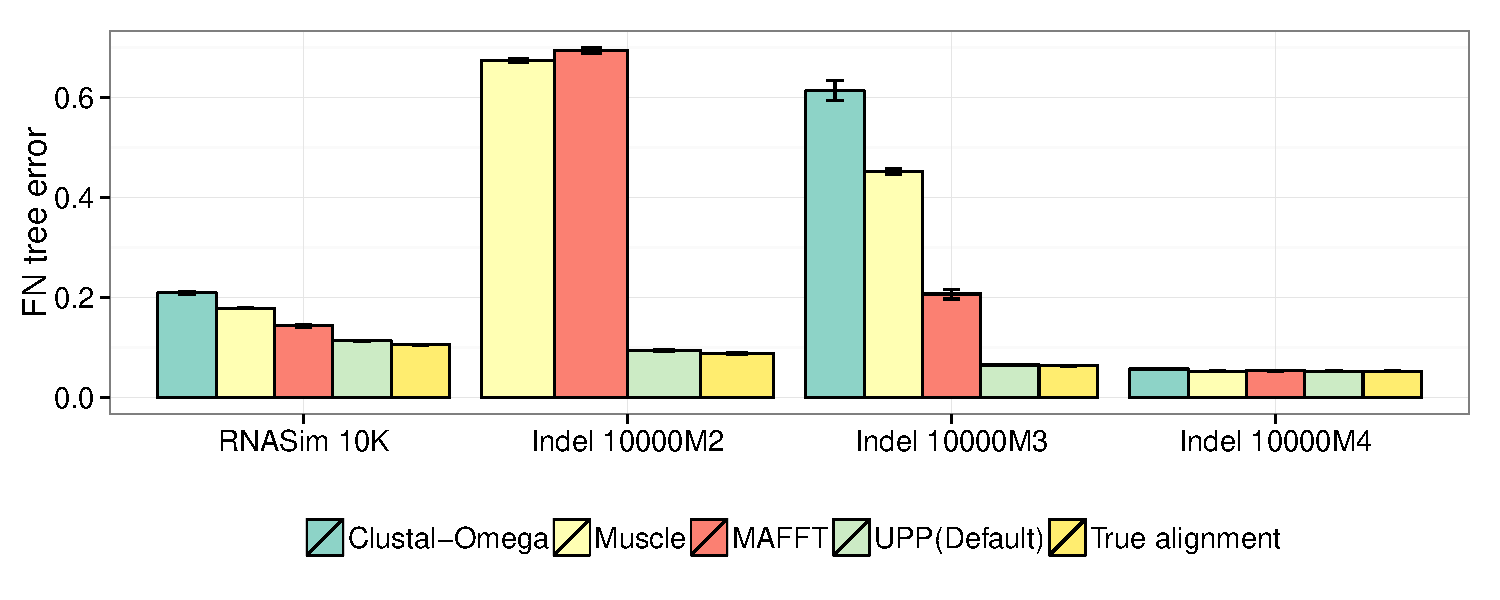
\includegraphics[width=0.9\linewidth]{{upp/large_sim.mixed.fn}.pdf}\\
\caption[Tree error on RNASim 10K and Indelible datasets]{\label{large_sim}  
{\bf Tree error on simulated datasets with 10,000 sequences.}  
I show FN tree error results on the RNASim 10K and Indelible datasets.  ML trees were estimated using FastTree under the GTR model.  All MSA methods were run with 24 GB of memory and 12 CPUs and given 24 hours to complete. MAFFT was run under the default setting on all datasets.  Standard error bars are shown.  Averages are computed over 10 replicates per dataset.  Clustal-Omega terminated with an error message on the Indelible 10000M2 datasets and thus, results are not shown.
%Muscle fails to run on datasets with 50K sequences or more due to 
%insufficient memory.  Similarly, MAFFT-profile(Fast) fails on the 200K dataset due to insufficient memory.  Clustal-Omega fails to generate an alignment within the 24 hour time limit on datasets with 50K sequences or more.  FastTree  completes within 24 hours on all tested alignments.  
}
\end{figure}

\paragraph{Impact of MSA estimation technique on phylogenetic tree estimation. }
Next, I evaluated the impact of MSA estimation on
phylogenetic tree estimation.
I show results for three of the 1000-sequence
model conditions,  each with
medium gap lengths, and varying the rate of evolution.
Under relatively low rates of evolution (1000M3), error
rates were generally low, but under moderate (1000M2) to
high (1000M1) rates of evolution, the tree error rates
increased for most methods
(fig.~\ref{1000_taxon_main_tree}).
For example, 
%UPP(Default) had the lowest tree error, with 
%$\Delta$FN ranging from 0.1-4.2\% under all nine model conditions.
on the hardest model condition (1000M1),
 the $\Delta$FN error
rates were 4.2\% for UPP(Default), 
%Nam - check this
%Done
15.4\% for MAFFT-L-INS-i, 20.5\% for Opal, 26.5\% for Muscle, and 
52.0\% for Clustal-Omega.
At the other extreme, on a very easy model condition (1000M3),
$\Delta$FN error rates were generally good:
0.2\% for UPP(Default), 
1.7\% for MAFFT-L-INS-i, 1.8\% for Opal,
and 3.7\% for Muscle; only  Clustal-Omega 
did poorly under this model condition (11.4\% $\Delta$FN).

Most methods do well  on the 5000-sequence simulated  AA datasets,
except for Opal, which failed
to align the COG438 dataset 
(terminated early due to memory error) and 
had high $\Delta$FN (12.2\%) on the other
datasets;
in comparison,
UPP(Default) had the most accurate results
(1.9\% $\Delta$FN), %Nam
followed by Muscle with 3.1\% and 
Clustal-Omega with 4.1\% %Nam?
(fig.~\ref{fasttree_main_tree}).
%Nam: Done

Performance on the Indelible and 
RNASim  datasets with 10,000 sequences (Fig.~\ref{large_sim})
show that UPP(Default)  
had very low FN error, within 0.7\%  tree error of ML on 
the true alignment, even on the hardest Indelible datasets.  
With the exception of the easiest Indelible model conditions
where all methods perform equally well (within 0.4\% tree error of ML on tree alignment), 
the other methods produced significantly less accurate trees.  
For example, on the Indelible 10000M2 model, 
UPP had 0.6\% $\Delta$FN error,
 MAFFT had 58.1\%, Muscle had 58.6\%,  and 
Clustal-Omega failed to generate an alignment 
(Fig.~\ref{large_sim} and section \ref{early_termination}).  
%Nam: updated MAFFT-Default tree error March 16th
  
I computed ML trees using
FastTree on three UPP alignments 
(UPP(Fast), UPP(Fast,NoDecomp), and  
UPP(Default,NoDecomp))
of the million-sequence RNASim dataset.
Despite the large number of 
sequences and relatively few sites (1500 average
sequence length), 
FN tree error was 
still very low: 8.4\% for UPP(Fast,NoDecomp),
 7.7\% for UPP(Default,NoDecomp),   and 7.5\% for UPP(Fast),
so that $\Delta$FN was between
2.0-2.8\% for all UPP variants I tested.
%(Figure \ref{fig:million}).  %fast with decomposition), with UPP(Fast) resulting in the lowest tree error.  
The phylogenetic accuracy  of these
trees is noteworthy, given that the  % both UPP(Fast) and
true alignment; see Table~\ref{alignment_large}) given
sequences were not particularly long  (1500 sites, on average),
indicating not only the quality of the
sequence alignment produced by UPP(Fast) and UPP(Fast,NoDecomop), but
FastTree's ability to produce reasonable results on
extremely large datasets.
%Tandy, Nam, Siavash - note this is not GTR evolution
%Nam, fill in value for UPP(Default,no-decomp) when available (March 6)
%Results on other datasets show
%similar trends (see SOM~\ref{upp_variant}). %Tandy - give location
%Nam:  Add in this section, currently only have UPP variants on RNASim
%New results for new backbone protocol on Gutell not done yet


I used the RNASim datasets to explore the 
impact of increased taxon sampling, which  is expected to improve
phylogenetic accuracy \cite{zwickl_increased_2002}.
As expected, tree error was reduced with increased
taxon sampling when using 
true alignments:
ML trees had  
FN error rates of
10.6\%, 8.1\%, 6.9\%, and 6.1\% on the RNASim 10K, 50K, 100K, and 200K datasets, 
respectively. % (Table \ref{table:XXX}).
I then tested this on the UPP alignments, to see if the
 beneficial impact
held for alignments estimated using UPP.
Maximum likelihood trees computed on 
UPP(Fast) alignments also reduced in error 
with increasing numbers of taxa:
UPP(Fast) trees had 11.8\% FN error
at 10K sequences, 9.4\% at 50K
sequences, 8.3\% at 100K sequences, 7.6\% at 200K sequences, and
7.5\% at 1,000,000 sequences.
%Nam - need to know where the results on the true alignment are
%provided - and also for the million sequence dataset
%perhaps add them to Table 1?
Thus, UPP alignments are good enough to show the beneficial
impact of increased taxon sampling on phylogenetic accuracy (similar
patterns hold for other UPP variants, see Table \ref{table:rnasim_upp_variants}).
%Nam, add something for UPP(Fast,NoDecomp), UPP(Default,NoDecomp), etc?
% \cite{zwickl_increased_2002}. 


\subsection{Structural alignment accuracy}

I used biological datasets with structurally-defined reference
alignments to evaluate UPP with respect to structural alignment
accuracy.
On the ten amino-acid datasets (10 AA) with
full alignments, 
Muscle had the highest average alignment error (30.2\%)
and the other methods (MAFFT-L-INS-i, Opal, 
and UPP) have very close
error rates between 23.5\% and 24.3\% (Fig.~\ref{align_error}(c),
figs.~\ref{balibase_main_alignment_mean}
and \ref{balibase_main_alignment_sop}).  
 % and \ref{balibase_main_tree} for full results.
The 19 HomFam datasets and three CRW datasts are too
large for MAFFT-L-INS-i or Opal, and so I use
MAFFT-Default (or MAFFT-PartTree on CRW 16S.B.ALL) on these data.
On the 19 HomFam datasets, 
Muscle failed to align
two datasets, and had generally very
high error on those it could align;
the other methods succeeded in 
aligning all the datasets. 
Comparing methods on just the 17 datasets 
that Muscle succeeded in aligning, 
UPP had 22.5\% alignment error, followed by
MAFFT-Default with 25.3\% error, 
Clustal-Omega with 27.7\% error, %Nam???
%Nam: Updated with Mafft-Default resutls
and Muscle with
48.1\% average error
%Nam: corrected
(Fig.~\ref{align_error}(c),
see also figs.~\ref{homfam_main_alignment} and \ref{homfam_main_spfn_spfp}
for additional results). 
%Nam, did you try to run MAFFT-default on HomFam?
%Yes, results are now in
MAFFT-default failed to run
on the 16S.B.ALL CRW dataset
(see Section \ref{early_termination}),
and so I used MAFFT-PartTree for that dataset; however,
I report
MAFFT-default for 16S.3 and 16S.T.
UPP   had the lowest average alignment error across
these three datasets (16.3\%), 
MAFFT had 28.8\%, 
Muscle had 30.7\%, and
Clustal-Omega  had 43.3\% (Fig.~\ref{align_error}(c)).
% was run using default setting for 16S.3 (25.2\% alignment
%error) and 16S.T (30.4\% alignment error),
%but could not be run in that setting on the
%16S.B.ALL dataset; hence, I report 
%MAFFT-PartTree (29.4\% alignment error).
%Note:  Mafft-Default does better on 16S.T, may be better than PartTree on CRW
% currently running it on 16S.B.ALL so once that's done numbers may change
Overall, UPP had the the best or close to the best results 
on these biological datasets, showing 
that UPP produced excellent alignments  
according to structural benchmarks on both nucleotides and amino acid sequences.
%gives good results on both nucleotide and amino acid datasets.
%However, Clustal-Omega did better on
%amino acid datasets than on nucleotide datasets, and
%Muscle did better on nucleotide datasets than on amino acid datasets.
%Nam, Siavash,  and Tandy - put this into the discussion 

\begin{figure}[htpb]
\begin{subfigure}[htpb]{\textwidth}
  \centering
  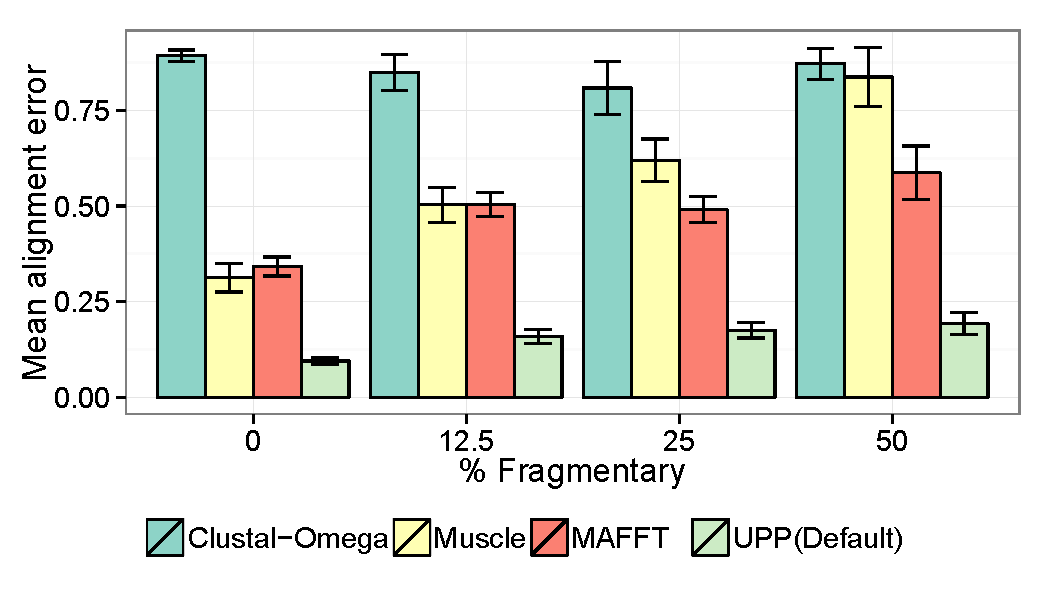
\includegraphics[width=0.85\linewidth]{{upp/frag.1000M2.alignment_average.main.500}.pdf}\\  
  \caption[]{Fragmentary 1000M2 model conditions}
\end{subfigure}
\begin{subfigure}[htpb]{\textwidth}
  \centering
  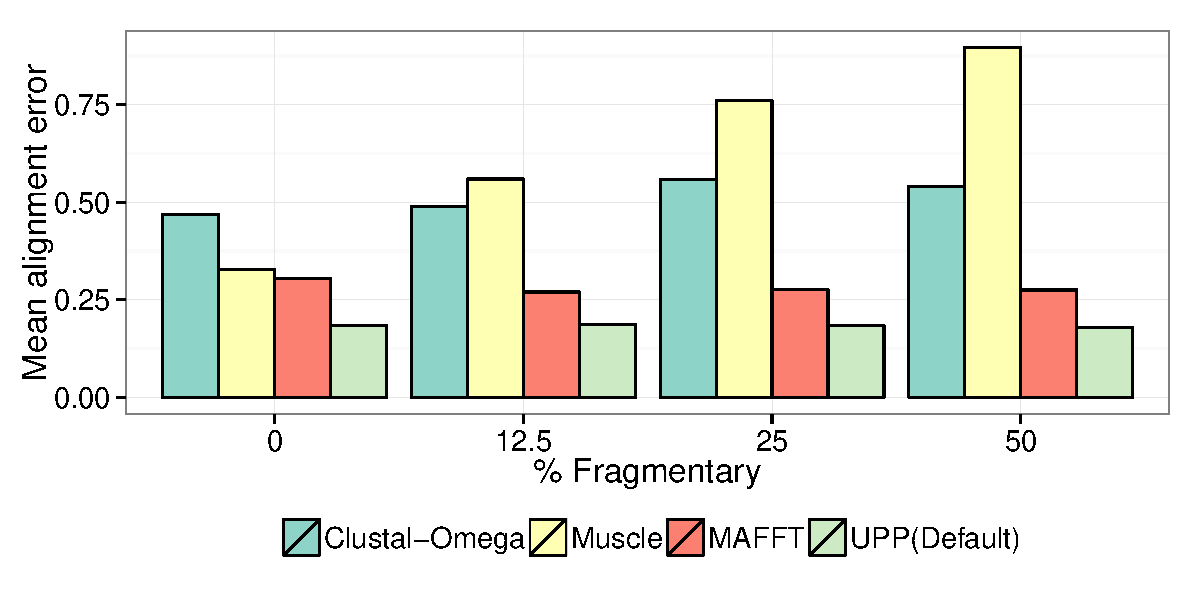
\includegraphics[width=0.85\linewidth]{{upp/frag.16S.T.alignment_average.main.500}.pdf}\\  
  \caption[]{Fragmentary CRW 16S.T datasets}
\end{subfigure}
\caption[Impact of fragmentary sequences on alignment error.]{\label{fig:fragmentary}  
{\bf Impact of fragmentary sequences on alignment error. }
I show alignment error rates for different methods on 
the 1000-sequence 1000M2 datasets and the 7350-sequence CRW 16S.T  
dataset, but include results where a
percentage of the sequences are made fragmentary, varying
the percentage from 12.5\% to to 50\%.
Fragmentary sequences have average 
length 500 
(i.e., approximately half the average sequence length for 1000M2,
and approximately one third the average sequence length for 16S.T).  
MAFFT is run using L-INS-i on the 1000M2 datasets and
using MAFFT-Default on the 16S.T datasets. 
} 
\end{figure}
\subsection{Results on fragmentary datasets. }
Figure \ref{fig:fragmentary} shows alignment
error on fragmentary
versions of the 1000M2 simulated datasets and the
CRW 16S.T biological dataset, varying
the percentage of fragmentary sequences from 0\% to 50\%, with
average fragment length 500 (roughly half the length of the full-length 1000M2 sequences and one third the length of the full-length 16S sequence). 
UPP(Default) had substantially lower error than the other
methods, at all levels of fragmentation for both datasets.
In most cases, alignment
error  increased  as the amount of fragmentary data
increases, but methods differed in their responses.
Muscle was the most impacted by 
the amount of
fragmentary data, with
very large increases in alignment error
as the amount of fragmentary data increases.
MAFFT-default
was  also impacted, but not as
severely as Muscle.
UPP and 
Clustal-Omega were largely unaffected by
fragmentation on these data (with error rates
that change only in small ways); however,
Clustal-Omega had poor accuracy consistently,
while UPP had consistently good accuracy.
Interestingly, the relative performance
of methods changed with the amount of
fragmentation; for example, 
Muscle was more accurate than 
Clustal-Omega on the
16S.T dataset before I introduce fragmentation,
but less accurate when 12.5\% of the
sequences were fragmentary (Fig.~\ref{fig:fragmentary}(b)).
Differences between methods were reduced on
model conditions with lower rates of evolution, but
UPP(Default) still demonstrated greater robustness to 
fragmentary data than the other methods (SOM~\ref{sec:all_frag_methods}).

Phylogenetic accuracy was also impacted by 
fragmentary data, but responses varied by the alignment method.
Results on the RNASim 10K datasets (Fig.~\ref{tree-frag})
with fragmentation varying from 0\% to 50\%, and
all fragments of length 500 (i.e., about one third of
the average length of the full-length sequences)
show that UPP(Default) and MAFFT-default were both
highly robust to fragmentary data ($\Delta$FN error rates 
only changing by 3\% for UPP and 2\% for MAFFT-default).
In contrast,  tree errors for Clustal-Omega and Muscle were very 
impacted by fragmentation.
Muscle had 7.3\% $\Delta$FN on full-length sequences,
and then 35.6-49.0\% $\Delta$FN under all the fragmentary
conditions.
Clustal had 9.1\% $\Delta$FN on full-length sequences,
and then 25.4\%-25.8\% on the fragmentary conditions.
Furthermore, while both UPP(Default) and MAFFT-default
were highly robust to fragmentary data, UPP(Default) had better
accuracy under all levels of fragmentation on
this model condition: 0.8\% $\Delta$FN on
full-length sequences, and at most 3.9\% $\Delta$FN
even when half the sequences are fragmentary.
MAFFT-default had 5.9\% $\Delta$FN for full-length
sequences, and $\Delta$FN between 5.8\% and 7.1\%
on the fragmentary sequences.

\begin{figure}[htpb]
  \centering
  %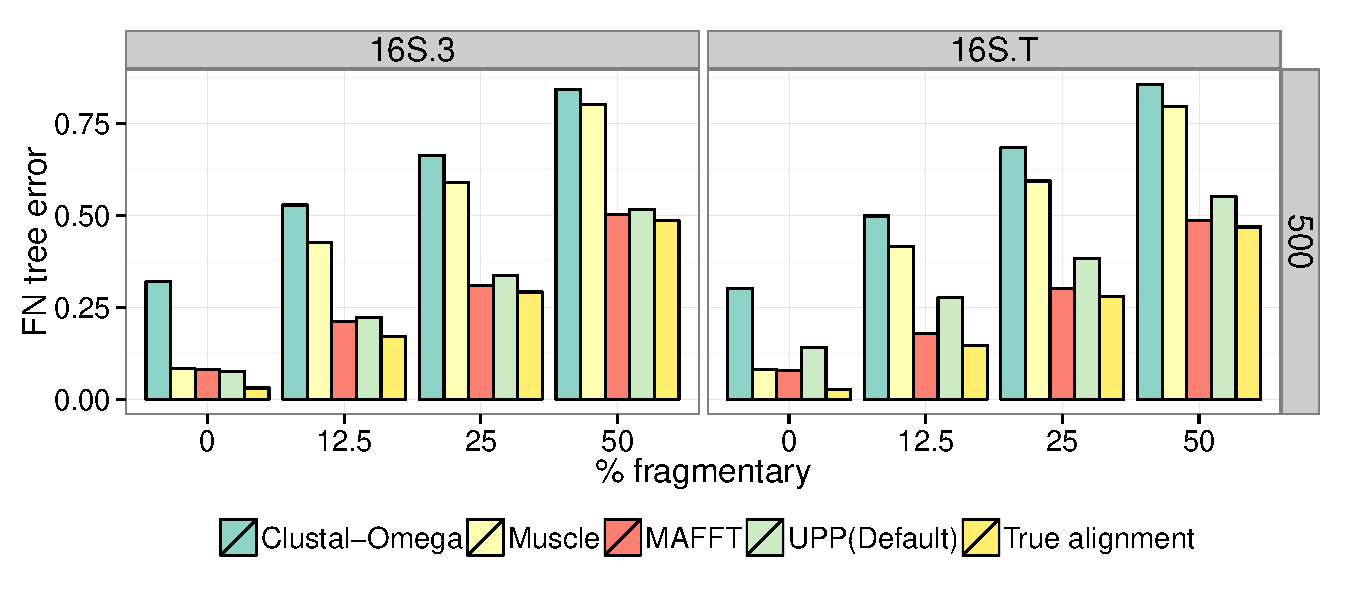
\includegraphics[width=0.90\linewidth]{{upp/large_fragmentary.gutell.fn.main}.pdf}\\
  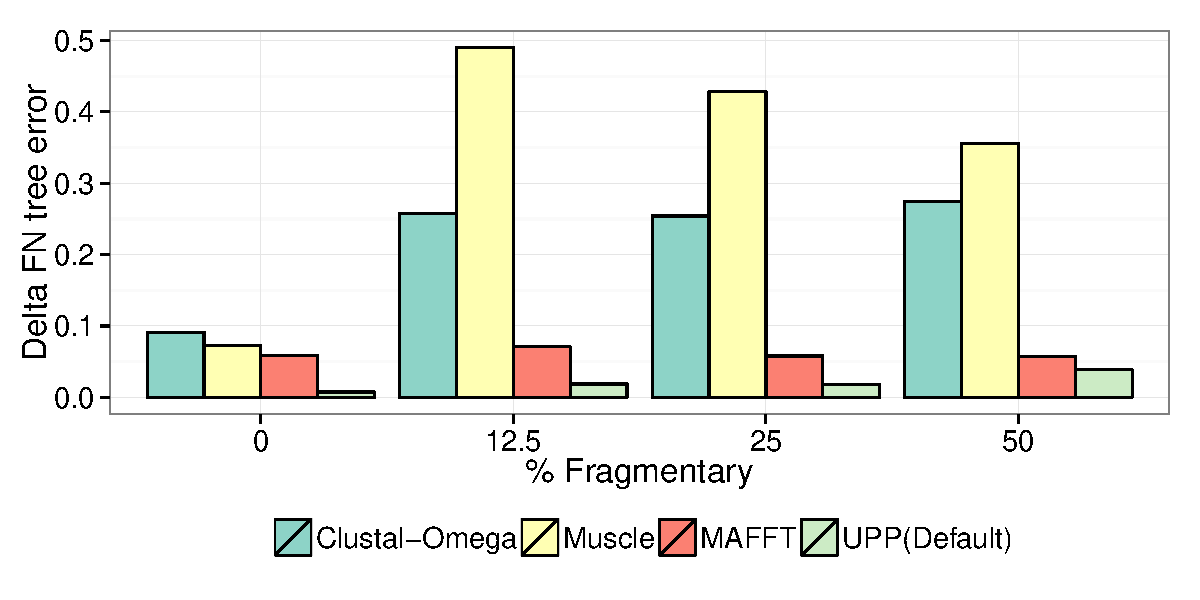
\includegraphics[width=0.90\linewidth]{{upp/frag.10000.delta_fn.main.500}.pdf}\\
  \caption[Tree error on fragmentary RNASim 10K datasets]
{\label{tree-frag}
{\bf Impact of fragmentation on tree error for the RNASim 10K datasets. }
I show the $\Delta$FN  error rates of
maximum likelihood  trees computed using FastTree under
the GTR model on
alignments computed using Clustal-Omega, Muscle,
MAFFT-Default, and UPP(Default), on the
RNASim 10K dataset, including results on versions of the
dataset where I make some of the sequences fragmentary.
All fragments have average length 500, but I vary the percentage of the
dataset that is fragmentary.
%Nam - would be better if I had RAxML, but I guess
%that will have to wait.
%Also, are these MAFFT-PartTree or MAFFT-Default?
}
%Nam - would be better to show Delta-FN.
%might also be good to include results on full-length sequences.
%also, order them in terms of increasing levels of fragmentation,
%just like you did for the alignment error.
%I will fix this
\end{figure}



Figure \ref{fragmentary_1000_taxa_tree} shows
similar trends for the 
fragmentary 1000M2
and 1000M3 datasets.
% but MAFFT (run using the most
%accurate setting, L-INS-i) is not as robust to fragmentation.
$\Delta$FN on the fragmentary 1000M2 datasets
ranged for UPP(Default) from 2.5-4.7\%,
from 34.7-65.0\% for Muscle,
and from 55.8-70.8\% for Clustal-Omega (fig.~\ref{fragmentary_1000_taxa_tree}).
Results on fragmentary versions of the 1000M3 model 
condition, which has a lower rate of
evolution than 1000M2, show $\Delta$FN for UPP(Default)
ranging from 0.2-2.2\%,
while $\Delta$FN ranged from 12.7-27.8\% for
Muscle and from 18.8-57.2\% for Clustal-Omega.
MAFFT-L-INS-i showed somewhat
better tolerance to fragmentary
data than Clustal-Omega or Muscle, but still
had high $\Delta$FN rates: 18.1-43.5\% error on the 1000M2 model condition, and 4.0-14.1\% for 1000M3.

\subsection{Factors influencing accuracy}
%Using the HMM Family technique instead of a single HMM
%produced a large impact on tree estimation error (Table 1
%and figs.~\ref{rnasim_upp_tree} and ~\ref{gutell_upp_tree}), but
%had a smaller impact on alignment error (figs.~\ref{rnasim_upp_alignment} and ~\ref{gutell_upp_alignment}).
The choice of alignment method
to compute the backbone alignment has an impact on final alignment and
tree accuracy:
comparing PASTA, MAFFT-L-INS-i, Muscle, and Clustal-Omega
for backbone alignment estimation, I found that
PASTA and Muscle backbones yielded the best alignment accuracy
(fig.~\ref{rnasim_alignment_alignment}) 
but PASTA and MAFFT-L-INS-i backbones yielded the best tree accuracy
(fig.~\ref{rnasim_alignment_tree}).
The choice of technique used to align query sequences
to the backbone alignment also impacts alignment and tree error
(Table 1 and figs.~\ref{rnasim_backbone}, \ref{rnasim_upp_tree}, \ref{gutell_upp_tree},
\ref{rnasim_upp_alignment}, and \ref{gutell_upp_alignment}), with the HMM Family technique giving
the best results compared to a single HMM or MAFFT-Profile with
either -{}-add or -{}-addfragments.

I found that the error of 
the backbone alignment and the 
alignment generated by three different ways of running UPP 
(default setting, and aligning query sequences using MAFFT-Profile)
were strongly correlated
(Fig.~\ref{backbone_error},
Pearson’s correlation coefficient 0.897; p-value=2.29e-10). 
Furthermore,
alignment errors for UPP(Default)  were
very close to the backbone alignment error, with root mean square difference (RMSE)
of 0.020, and 
closer to the backbone alignment error than those
produced by UPP using MAFFT-profile 
(RMSE of 0.024 for MAFFT-profile-{}-addfragment
and 0.051 for MAFFT-profile-{}-add, fig.~\ref{backbone_error}).
%in alignment error of 0.020 for UPP versus 0.024 and 0.051 for MAFFT-profile “addfragments”
%and MAFFT-profile “add”).
Thus, while the three versions of UPP all showed
good correlations between backbone alignment error and 
final alignment error, 
the use of the HMM Family
technique gave the best correlation, and helps
UPP to scale alignment accuracy obtained on
small subsets to large datasets.







\subsection{Running time. }
%Nam - can you give running times (approximately) on other datasets, not just RNASim?
%Nam: I can get numbers for Gutell, remove this note once done

\begin{figure}[htpb]
%\begin{subfigure}[htpb]{\textwidth}
  \centering
  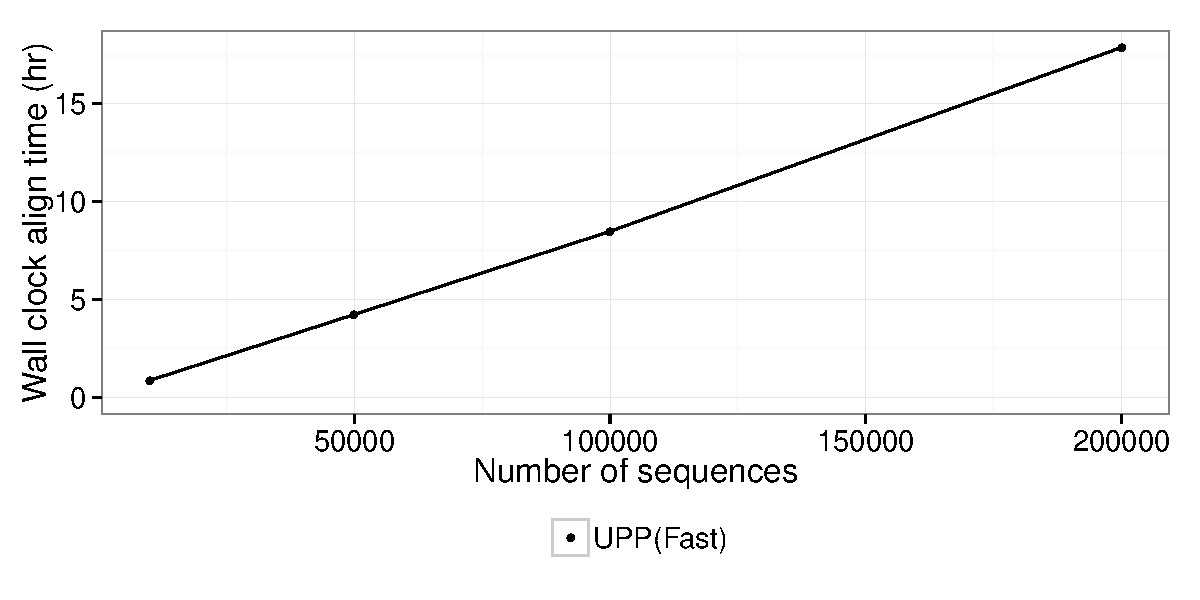
\includegraphics[width=0.95\linewidth]{{upp/rnasim.only_upp.wall_align_time}.pdf}\\
 % \caption[]{Wall clock alignment time (hr)}
%\end{subfigure}
\caption[Running time for UPP(Fast) on the RNASim  datasets.]
{\label{running-time}  {\bf Running time for UPP(Fast) on the RNASim
datasets. }
I show running time for UPP(Fast) on RNASim datasets
with 10K, 50K, 100K, and 200K sequences.
UPP(Fast) uses a backbone of size 100, computes the backbone
alignment using PASTA, and then aligns the remaining sequences
using the HMM Family technique.
All analyses were run on TACC with 24 GB of memory and 12 CPUs.
%MAFFT is run using the PartTree command on all these datasets.
%Results not shown are due to methods failing to return an alignment
%within the 24 hour time period on TACC, using 12 processors.
% Muscle fails to run on datasets with 50K sequences or more due to insufficient memory.  Similiarly, MAFFT-profile(Fast) fails on the 200K dataset due to insufficient memory.  Clustal-Omega fails to generate an alignment within the 24 hour time limit on datasets with 50K sequences or more.  
}
\end{figure}
%Nam - remove "Method"
%Nam: done


\begin{table}[htpb]
\caption[UPP variants on the RNASim datasets.]{\label{table:rnasim_upp_variants}
{\bf Results for UPP variants on the RNASim datasets.}
I show results for different
variants of UPP on the RNASim datasets with 10,000 to 200,000
sequences. 
I report the average alignment error, 
$\Delta$FN error (the difference
between the error on the true alignment
and on the estimated alignment), 
and running time (in CPU hours), using
12 processors with 24Gb of memory.
The default setting for UPP is denoted
Default; it uses a backbone of size 1000, uses PASTA 
to compute the backbone alignment, and the HMM Family technique;
Fast is obtained by using backbones of size 100 and keeping
all other settings constant.
The ``ND'' versions of these two methods replace the HMM Family
technique with a single HMM.
Default-MP uses MAFFT-Profile (with -{}-add, denoted ``A'',
or with -{}-addfragments, denoted ``AF'') to add the query sequences into the
backbone alignment, and otherwise is identical to Default;
Fast-MP differs from this only by using
a backbone of size 100.
}
\centering
\scalebox{0.90}{
\begin{tabular}{|l|l|r|r|r|r|}
\hline
Number seq. &Method&Align.~error&FN&$\Delta{FN}$&Time (hrs)\\
\hline
10,000&Fast-ND&13.1\%&14.2\%&3.6\%&0.1\\
10,000&Default-ND&11.2\%&13.6\%&3.0\%&0.2\\
10,000&Fast&13.3\%&11.8\%&1.2\%&0.9\\
10,000&Default&10.3\%&11.4\%&0.8\%&6.7\\
10,000&Fast-MP-A&26.2\%&18.0\%&7.4\%&0.2\\
10,000&Default-MP-A&14.0\%&14.8\%&4.2\%&0.3\\
10,000&Fast-MP-AF&17.8\%&15.5\%&4.9\%&1.0\\
10,000&Default-MP-AF&12.7\%&12.3\%&1.7\%&6.5\\
\hline
50,000&Fast-ND&12.2\%&10.7\%&2.6\%&0.4\\
50,000&Default-ND&12.0\%&10.5\%&2.5\%&0.9\\
50,000&Fast&12.7\%&9.4\%&1.3\%&4.2\\
50,000&Default&11.2\%&8.6\%&0.5\%&44.0\\
50,000&Fast-MP-A&33.6\%&13.8\%&5.7\%&2.1\\
50,000&Default-MP-A&16.0\%&10.1\%&0.2\%&3.5\\
\hline
100,000&Fast-ND&13.5\%&9.9\%&3.3\%&0.8\\
100,000&Default-ND&11.2\%&9.4\%&2.8\%&1.9\\
100,000&Fast&13.0\%&8.3\%&1.4\%&8.5\\
100,000&Default&11.1\%&7.6\%&0.7\%&82.3\\
100,000&Fast-MP-A&40.2\%&10.2\%&3.3\%&10.7\\
\hline
200,000&Fast-ND&12.4\%&8.5\%&2.4\%&1.9\\
200,000&Default-ND&11.3\%&8.6\%&2.4\%&6.1\\
200,000&Fast&12.5\%&7.6\%&1.4\%&17.9\\
200,000&Default&10.6\%&6.8\%&0.7\%&151.1\\
\hline
\end{tabular}}
\end{table}

Running times for UPP(Fast) on the RNASim datsets
with up to 200,000 sequences, using 12 processors,
show a close to linear trend, so that
UPP(Fast) completes on 10K sequences in 55 minutes, 
on 50K sequences in 4.2 hours,
on 100K sequences in about 8.5 hours,
and on 200K sequences in about 17.8 hours (Fig.~\ref{running-time}).
Table \ref{table:rnasim_upp_variants} explores
the trade-off between running time and 
accuracy (both alignment and tree)  of 
UPP variants.
For example,  using UPP(Fast) instead of UPP(Default)
reduces the running time substantially (by a factor
of 7 to 10) and produces only a small
increase in tree error and 
alignment error.
However, UPP is extremely parallelizable, and so
speed-ups are easily achieved through increasing
the number of processors.

\section{Conclusion and future work}\label{upp:conclusion}
Although the relative  performance
of multiple sequence alignments 
varied by datasets,   UPP in most cases showed improved alignment accuracy compared
to PASTA, SAT\'e-II, Clustal-Omega, Muscle, 
and MAFFT. 
By design, 
UPP(Default) is identical to PASTA on datasets without fragments and at most 
1000 sequences, but UPP is highly robust to fragmentary data whereas PASTA is not. 
On larger datasets,
UPP alignments tend to be more accurate than PASTA alignments, 
but ML trees based on PASTA alignments (for fragment-free datasets) are typically
more accurate than ML trees based on UPP alignments. 
However, on large datasets, 
ML trees estimated on UPP alignments are typically more accurate than 
ML trees based on all other methods (including SAT\'e-II). 
Moreover, for datasets with fragmentary sequences,
UPP provided the best alignment and tree accuracy of all the methods I tested.
Finally, UPP was the only method I tested that was able to analyze the million sequence RNASim dataset. 

UPP exhibits great scalability, both with respect to
running time (which scales in a nearly linear manner)
and parallelism, but also with respect to alignment accuracy.
For example, my study showed the alignment error on the backbone alignment is quite close to the alignment error on the alignment
returned by UPP(Default) (Section~\ref{backbone_alignment_error}), 
and this close relationship between the accuracy of the backbone alignment
and the final alignment is weaker when I use MAFFT-Profile
second iteration) and I didn't fully explore using a single HMM other than RNASim
instead of an HMM Family to align query sequences. 
Thus, the HMM Family technique is a key algorithmic 
technique to providing scalability for alignment accuracy, so that
large datasets can be aligned nearly as accurately as smaller datasets.  

However, the other algorithmic techniques also contribute to 
UPP's improved accuracy.
Restricting the backbone to full-length sequences improves
the robustness to fragmentary sequences, and
the re-sampling technique improves the close relationship between the
backbone alignment accuracy and the final alignment accuracy.
Using PASTA for the backbone alignment gives better results
than using less accurate alignment methods, 
and because PASTA is computationally efficient it also
makes it feasible to use large backbones.
Thus, the different algorithmic steps work together to
provide the improved accuracy, scalability, and robustness
to fragmentary sequences.
Furthermore, while good accuracy with respect to
structural benchmarks
was achieved using simpler versions of UPP (e.g.,
using MAFFT-L-INS-i instead of PASTA for the backbone alignment,
or using a single HMM rather than the HMM Family Technique to
align query sequences), 
the best accuracy was
obtained using my default setting, 
which also gave better results on the phylogenetic benchmarks.
Thus, UPP has excellent accuracy with respect to 
both phylogenetic and structural benchmarks, indicating
that alignments produced by UPP are highly accurate 
with respect to  positional homology and also structural homology (see
\cite{Reeck1987} for further discussion of these 
related but different concepts).

By design,
UPP is a highly modular algorithm, 
and substitutions in its algorithmic steps could lead to additional
improvements.  Because my results show that  
using small backbones
reduces accuracy only slightly, this opens the possibility of 
using sophisticated but computationally intensive
multiple sequence
alignment methods (for example, 
statistical methods based on stochastic models of sequence evolution involving
indels \cite{rs06,jordan-pnas2013}) 
to produce the backbone alignment.
The HMM Family technique is another part of
this pipeline that could be improved, for example
through using new techniques to compute HMMs (which might incorporate
structural information) or to add query 
sequences to alignments (another active area of research).  
Thus, UPP is an algorithmic paradigm rather than a specific
method, and future work will explore the design space enabled by
this paradigm.

In summary,  UPP enables highly accurate analyses of
sequence datasets that have been considered too difficult
to align, including
datasets that evolved with high
rates of evolution,   that
contain fragmentary sequences, or that are very large. 
While datasets
like these are increasingly being generated in large-scale
sequencing projects, 
the limited ability to analyze these datasets has discouraged
biologists from using the full range of their data. 
Instead, large-scale transcriptomic
and genomics projects often sub-sample from the available data
(in terms of taxa, genomic regions, and sites within genes)
in order to obtain datasets that are small enough, 
that evolve sufficiently slowly, and that do
not contain fragmentary data, so that 
available MSA methods can be reliably run on these datasets.
% Tandy, Nam, see if you agree with this addition.
% (I don't feel strongly about including this at all) 
%Therefore, UPP's increased MSA accuracy
%even on large datasets with high evolutionary rates
%enables the use of more data 
%in downstream analyses such as phylogenetic reconstruction.
%however, whether including more data 
%improves those downstream analyses
%likely depends on the application,
%and requires careful study. 
%Siavash - I took it out because the main point is in the next paragraph

UPP's robustness to fragmentary data, and its high
accuracy even for ultra-large datasets with
high rates of evolution,  
increases the range of genomic data that can be 
used in scientific studies.
As a result, scientific questions that would be improved through 
larger sequence datasets
might be able to be addressed with greater accuracy
using UPP. A prime case of where UPP could be useful is
for phylogeny estimation of
rapid radiations or deep evolution, since phylogeny estimation
 is often improved by
dense taxon sampling \cite{zwickl_increased_2002}. 
For example, the avian genome project is planning to 
eventually sequence all roughly 10,000 living bird species,
and such efforts require scalable and accurate alignment 
techniques such as UPP. % and PASTA?
However, datasets
on  smaller numbers of taxa can also
%be extremely large for multi-copy genes, 
include extremely large multi-copy gene families
(e.g., the 1KP  gene sequence datasets for 
1000 species and more than 100,000 sequences). 
Understanding the evolutionary history of these large gene families
requires gene family trees  and alignments, 
that can easily involve many tens of thousands of
sequences.
Thus, UPP is a tool for both current and future genomics and
transcriptomics projects, that will  enable
biologists to utilize the full range of their data to 
address biological problems of broad interest.


% \subsection{Comparison to previous work. }
% MSA estimation for the purpose of structure and function
% prediction
% of protein sequences (and in some cases of RNA sequences)
% is often based on machine learning models such as
% templates or profile Hidden Markov
% Models (HMMs) \cite{Eddy1998}.
% These models are used  to represent a
% seed alignment (typically
% a curated structural alignment) for the
% molecule, which is then coupled with
% methods, such as HMMALIGN \cite{HMMER} and
% MAFFT-Profile \cite{Katoh2012}, to add the
% input sequences
% into the seed  alignment and  produce
% a final multiple sequence alignment.
% Similarly, profile HMMs for different protein
% families and superfamilies are provided in
% databases such as Pfam \cite{Punta2012} and
% PhyloFacts \cite{Krishnamurthy2006},  and
% can be used to
% build multiple sequence alignments.
% However,   these ``template-based" methods
% (e.g., \cite{neuwald2009,Nawrocki2009,ShangGardnerGutell})
% can only be used to align
% sequences that match the seed alignment, and so are not
% \emph{de novo} MSA methods.
% PROMALS \cite{promals}, SATCHMO \cite{satchmo03}, and SATCHMO-JS \cite{kimmen2010}
% are protein MSA methods that build HMMs during
% the course of the alignment estimation, and
% so can be used in \emph{de novo}
% alignment; unfortunately, these methods
% %these methods
% are computationally intensive because they
% perform a sequence of HMM-HMM alignments
% to construct their final alignment, and so
% cannot be used on large datasets.


% Phylogenetic placement is a related problem
% where profile HMMs have also been used:
 % the input is
% a set of query sequences and a reference
% tree and alignment, and the objective is
% to find an edge in the reference tree
% for each query sequence.   
% SEPP \cite{Mirarab2012} is a method for
% phylogenetic placement that 
% decomposes the reference tree into
% approximately ten disjoint subsets of sequences of 
% roughly the same size, builds a profile HMM on
% each subset alignment, aligns each query sequence
% to the backbone alignment using the best scoring profile HMM,
% and then finds the best location in the reference tree using
% pplacer \cite{Matsen2010}, a method that
% optimizes the position of the query sequence 
% within the reference tree
% under the
% ML criterion. 
% I modified SEPP so that it could be used as 
% a multiple sequence alignment method, using the
% backbone sequence alignment and tree computed by UPP as the
% reference alignment and tree.
% %Although subset size impacts accuracy, SEPP uses an \emph{ad hoc} rule for 
% %deciding the subset size -- it decomposes into subsets that are 
% %roughly 10\% the size of the backbone.
% %\ref{gutell_sepp_alignment}-\ref{fig:frag_sepp}
% Alignment error was not substantially
% different for UPP and SEPP (figs.~\ref{rnasim_sepp_alignment} and
% \ref{gutell_sepp_alignment});
% however, 
% trees computed using UPP on the 16S.3 and 16S.T CRW datasets
% were more accurate than trees computed using SEPP
% (fig.~\ref{gutell_sepp_tree}).
% %Nam - put in correct numbers
% %Nam: Numbers are corrected March 16
% For example, on 16S.3, SEPP(Default,10\%) had 6.8\% $\Delta$FN
% and UPP(Default) had 4.6\% $\Delta$FN.
% On 16S.T, SEPP(Default,10\%) had 15.3\% $\Delta$FN
% %while the first iteration of
% %UPP(Default) had 11.7\% $\Delta$FN, and the second
% and UPP(Default) had 11.5\% $\Delta$FN.  
% UPP was also
% more robust to fragmentary data than SEPP (fig.~\ref{fig:frag_sepp}).
% Thus,  UPP and SEPP had
% similar accuracy on fragment-free datasets with 
% at most
% moderate rates of evolution, but under
% other conditions UPP produced
% more accurate trees than SEPP.

\chapter{Conclusion and future work}\label{conclusion}
\index{Conclusion@\emph{Conclusion}}%

\section{Conclusion}
Sequence alignment is a vital step in many bioinformatic analyses.  From the alignment, the phylogenetic relationship between the different sequences in the alignment can be inferred.  Under the context of phylogenetic placement, I have shown that the HMMER approach of using a single HMM for aligning sequences to an existing alignment suffers when the sequences come from distantly related taxa, and that new methods are necessary for aligning evolutionarily divergent sequences.  I present such a technique in Chapter~\ref{hmmfamily}.  I describe the basic outline of the families of HMMs technique and how it can be used to align sequences to an existing backbone alignment.  

In Chapter~\ref{sepp_chapter}, I implemented the families of HMMs technique within SEPP and apply SEPP toward the phylogenetic placement problem.  I presented a simulation study and showed that SEPP resulted in better placement accuracy than HMMALIGN+pplacer and PaPaRa+pplacer on difficult datasets.  More importantly, I validated the hypothesis that using multiple HMMs can result in significantly better phylogenetic placement accuracy than using a single HMM.  This result forms the basis for the remaining chapters of my dissertation.

In Chapter~\ref{tipp_chapter}, I presented TIPP, an extension of SEPP by including statistical support measures, and showed its performance on  taxonomic identification and profiling.  I showed that using multiple HMMs resulted in better classification accuracy than using a single HMM.  Most interestingly, I showed that under the context of taxonomic identification, requiring a high statistical support threshold for classification resulted in the best overall results, however, under the context of taxonomic profiling, using the minimum support threshold resulted in the best overall taxonomic profiles.  Thus, the choice of the statistical support threshold depends on the application.

In Chapter~\ref{upp_chapter}, I presented UPP, a modification of SEPP for ``de novo'' sequence alignment.  SEPP requires a backbone alignment as input.  I presented a new technique to intelligently select the set of sequences to form the backbone alignment, and then applied the families of HMMs technique to complete the alignment on the entire set of sequences.  I showed that UPP typically resulted in better alignments on both DNA and amino acid sequences, which in turn, resulted in more accurate phylogenies compared to other methods.  In addition, I showed that UPP could accurately estimate an alignment on 1,000,000 sequences without the need of a supercomputer in less than 2 days.

\section{Future Work}
SEPP, TIPP, and UPP all use a similar pipeline for sequence alignment: a backbone alignment is decomposed into closely related subalignments using a phylogenetic tree, and the query sequences are aligned to the subalignments.  Any improvement to this pipeline could potentially result in improved accuracy in each of the three techniques.  Possible ways to prove the accuracy of the pipeline include:
  
\begin{itemize}
\item Testing different methods for aligning the query sequence to the backbone alignment.  For example, we saw in Chapter~\ref{upp_chapter} that Mafft-profile under the most accurate settings resulted in accurate alignments on datasets containing both fragmentary and full-length sequences, however, could not be run on the larger datasets.  The subalignments generated by the decomposition process could be made sufficiently small enough such that Mafft-profile could be run optimally.
\item Exploring different methods for decomposing the backbone alignment.  In all three methods presented, the backbone tree was decomposed using the centroid edge decomposition.  Using a different technique, such as the longest edge decomposition used in SAT\'{e}~\cite{Liu2009} may result in better HMMs.  Similarly, using a clade-based decomposition to group together taxonomically similar sequences may result in better HMMs.
\item More simulation studies comparing the hierarichal families of HMMs versus the the disjoint families of HMMs.  Currently, only UPP has been tested with the hierarichal families of HMMs.  However, more extensive studies comparing both techniques are necessary, both within SEPP, TIPP, and UPP.
\item Examining different parameter settings within the HMMER software suite.  By default, HMMBUILD collapses very gappy sites into one state in the HMM.  However, SEPP, TIPP, and UPP have this option disabled; each site with at least one non-gap character in the backbone alignment results in one state in the HMM.  Better performance may be obtained by allowing gappy sites to be collapsed.
\end{itemize}

There are several areas in which TIPP can be further improved.
\begin{itemize}
\item Expanding the marker gene set.  TIPP currently uses a set of 30 marker genes for taxonomic profiling.  A simple extension would be to expand the marker gene set to the 40 marker genes used in~\cite{Sunagawa2013}, as well as update existing marker genes to include recently sequenced species.  By expanding the marker gene set, TIPP may be able to estimate more accurate profiles on metagenomic datasets.  
%\item Better curation of the marker set.  As Table~\ref{tipp:marker_stats} shows, the number of species per marker gene can range from 65 species to 1555 species.  Thus, some markers may 
\item Exploring taxonomic identification of viral sequences.  Viruses are difficult to identify because there are no genes that are found across all viruses.  Instead, viruses are typically identified using group specific genes.  To make the problem more difficult, viruses have high rates of mutations and horizontal gene transfer, making alignment estimation and phylogeny estimation difficult~\cite{todo}.  Thus, viral identification would be a good test case for TIPP's ability to classify divergent sequences.
\item Combining abundance profiles.  TIPP currently uses a simplistic algorithm for computing the taxonomic profile from the marker genes; all reads that are binned to any of the marker genes are pooled together, and the abundance profile is estimated on the pooled reads.  This process ignores the fact that the source gene of the reads is known.  Better profiles may be obtained if separate abundance profiles are estimated from the reads binned to each individual marker gene, and the profiles are combined using a mixture modeling approach.  
\item Improved detection of rare species in a sample.  One difficulty in taxonomic profiling is determining whether a low abundance species is truly present, or the abundance estimation is a false positive.  While TIPP treats each read independently, the reads themselves are not independent; they come from population of species present in the metagenomic sample.  Thus, inferences about the abundance profile of the reads can be used to filter out false positives, as well as detect rare species.  For example, if a rare species is detected across multiple different markers, it's likely to be present in the sample.  However, if the species is only present in very few markers, then it is more likely to be a false positive. 
\end{itemize}

Future work on UPP include:
\begin{itemize}
\item Incorporating iteration within UPP.  The quality of the final alignment can be heavily dependent on the initial selection of the backbone sequences.  The initial step of filtering short sequences from the backbone selection process may exclude entire clades from the backbone set, making it difficult to align sequences from the excluded clade.  I have already shown preliminary work that iteration within UPP can result in better alignments when the initial backbone set is sampled non-uniformly from the phylogenetic tree.  Re-sampling may also be necessary due to random sampling failing to include any sequences from smaller clades.  Better results could be obtained by examining different re-sampling strategies, as well as examining different ways of selecting the backbone set.  
\end{itemize}


%\textbf{Citations to include}

%\textbf{Nam:  rewrite the future work section.  Split into 4 sections:  general improvements that impact all 3 methods, and individual sections for SEPP, TIPP, and UPP sections.}


%%%%%%%%%%%%%%%%%%%%%%%%%%%%%%%%%%%%%%%%%%%%%%%%%%%%%%%%%%%%%%%%%%%%%%
% Appendix/Appendices                                                %
%%%%%%%%%%%%%%%%%%%%%%%%%%%%%%%%%%%%%%%%%%%%%%%%%%%%%%%%%%%%%%%%%%%%%%
%
% If you have only one appendix, use the command \appendix instead
% of \appendices.
%
\appendices
\index{Appendices@\emph{Appendices}}%

\makeatletter 
\renewcommand{\thefigure}{A\@arabic\c@figure} 
\makeatletter 
\renewcommand{\thetable}{A\@arabic\c@table} 
\makeatletter 
\renewcommand{\thesection}{A\@arabic\c@section} 
\newpage
\section{SEPP}
SEPP (SAT\'e-enabled phylogenetic
placement)  is used for one of 
the  major algorithmic
steps which TIPP.
We describe SEPP's strategy briefly here, but
see \cite{Mirarab2012} for full details.
We let $A$ be
the  reference alignment and $T$ the reference tree on the set $S$ of 
full-length sequences.

\noindent{\bf Step 1: Decomposition.}  
The parameters that govern the decomposition strategy are
$m_p$, the maximum size of the ``placement subsets", and
$m_a$, the maximum size of the ``alignment subsets".
SEPP requires that each alignment subset be a subset of
a placement subset, and so requires that $m_a \leq m_p$.
SEPP uses $T$ to
decompose the sequences in $S$ into 
disjoint placement subsets, and then decomposes
the placement subsets further (if $m_a < m_p$) into
disjoint alignment subsets, as follows.
SEPP finds a centroid edge in $T$ (one that
separates the leaf set into two sets of
approximately equal size), and breaks the tree accordingly into two subtrees.
For each resulting subtree that contains more than $m_p$ leaves, 
SEPP recursively repeats this decomposition.
This produces a partition of $S$  into subsets $S_1, S_2, \ldots, S_k$,
with each subset having at most $m_p$ elements.
If $m_a < m_p$, then the decomposition
process continues on any subset $S_i$ with more than $m_a$ leaves,
until each placement subset has been further partitioned into
disjoint
alignment subsets, each having at most $m_a$ leaves. 


\noindent{\bf Step 2: Compute Extended Alignment. }  
For a given alignment subset of sequences $S' \subset S$, 
we define $A'$ to be restriction of alignment $A$ to $S'$.
SEPP uses HMMER to compute an HMM $H'$ on $A'$ for each alignment subset
and to score $q$ with respect to each $H'$.
Thus, SEPP represents the backbone alignment with a set of
HMMs (a technique we call an ``HMM
Family).
HMMER produces measures of the fit between
each HMM and each query sequence called ``bit-scores" (discussed in
Section \ref{tipp:bitscores}).
Then,  for each query sequence $q$, the alignment
subset with the best bit-score is noted.
SEPP uses HMMER to align $q$ to the alignment
on the subset with the best bit-score, and
then extends the reference alignment $A$ on the full dataset to include $q$.
This is an ``extended alignment" for the query $q$;
thus, each query sequence $q$ gives rise to a different extended
alignment with $|S|+1$ sequences.

\noindent{\bf Step 3: Placement. }
The query sequence $q$ is placed in the reference tree
$T$
using the  preferred  placement method.
The current implementation of SEPP enables the use of both
pplacer and EPA for the placement of
fragments. EPA and pplacer 
have identical optimization criteria and
use very similar techniques:
both
place fragments to optimize maximum likelihood
using  
the GTRGAMMA model for DNA sequences or a selected protein model 
for AA sequences, and 
return a set of placements, each with
its confidence level. See Section \ref{supp:hmmer_epa} for more discussion
about EPA and pplacer, and a comparison of their
performance. 

As described, SEPP places fragments into the reference tree;
however, SEPP (and any
phylogenetic placement method) can be used to 
place fragments into any tree on the same set of sequences,
optimizing likelihood; this allows SEPP to use the
reference tree to divide the sequence dataset into
alignment subsets, and yet place 
the fragments into some other tree. 
This flexibility will be useful in developing TIPP.

\cite{Mirarab2012} found
settings for the
SEPP parameters that gave good accuracy in
reasonable time under a wide range of conditions; these were
$m_a=10$ and
$m_p=n$, where $n$ is the number of leaves in the reference alignment and tree.
Thus, small alignment subsets improve accuracy, and
placing in the entire tree improves accuracy.
However, when $n$ is very large, 
these settings are computationally expensive.
To reduce the computational challenges, SEPP limits the 
portion of the reference tree into which each query sequence can be placed;
this is the purpose of the parameter $m_p$.
Precisely, if the best alignment subset
for the query sequence is determined to be
$S^a$, 
then SEPP places $q$ into the subtree of
the reference tree defined by 
the leaves of $S^p$, where $S^p$ is the unique placement subset
containing $S^a$.
This defines a unique edge in the reference
tree into which to place the query sequence.
% (i.e. the subtree defined by the placement subset
%that includes the best-scoring alignment subset).

\section{TIPP on larger markers}\label{supp:large_marker}
We modified how we run TIPP on the bacterial 16S RNA
dataset due to the large number of taxa (9197),
as follows: we used the SAT\'{e} alignment
as the reference alignment, the
refined taxonomy as the reference tree, and rather
than placing into the entire refined taxonomy, we use
SEPP to decompose the refined taxonomy into both alignment
subsets and placement subsets using decomposition
parameters of $m_p=1000$ and $m_a=100$.  Thus, reads are
placed into subtrees of the 16S marker, each of which
contains at most 1000 leaves.


\section{Precision and Recall Comparisons and Statistical Significance}
In this section we compare techniques two at a time according to precision and recall.
For each comparison we show tables with differences between precision and recall values of the two techniques being compared,
and indicate whether the differences are statistically significant. 

\subsection{HMMER+pplacer versus HMMER+EPA}\label{supp:hmmer_epa}
Table \ref{tipp:difference.leaveout.rspb.pplacer.epa} shows that 
pplacer and EPA are indistinguishable in terms of both precision and recall
(i.e., the differences are not statistically significant).

\begin{table}[hptb]
\caption[Precision-Recall Differences between HMMER+pplacer and HMMER+EPA on the rpsB gene]{\label{tipp:difference.leaveout.rspb.pplacer.epa}
The difference between precision and recall of HMMER+pplacer and HMMER+EPA in the leave-species-out experiments on the rpsB gene. 
Negative values indicate HMMER+EPA is better, while positive values indicate that HMMER+pplacer is better.
None of the differences were statistically significant according to the Pearson's chi-square contingency table test (as implemented in R~\cite{R}).
p-values are shown in parentheses below each comparison.  
 }
\begin{center}
\begin{tabular}{|l||c|c|} \hline
\multicolumn{1}{|l||}{}&\multicolumn{1}{c|}{recall}&\multicolumn{1}{c|}{precision}\\ \hline
genus&~0.005&~0.008\\ 
&(0.535)&(0.386)\\ 
family&-0.001&-0.001\\ 
&(0.930)&(0.865)\\ 
order&~0.004&~0.004\\ 
&(0.525)&(0.517)\\ 
class&~0.005&~0.005\\ 
&(0.350)&(0.297)\\ 
phylum&~0.003&~0.004\\ 
&(0.405)&(0.329)\\ 
\hline
\end{tabular}
\end{center}
\end{table}


%========================= Experiment 1 ======================


\subsection{Experiment 1: TIPP variants}\label{supp:tipp_variants}
In this section we provide comparisons of different TIPP variants. 
\subsubsection{HMMER+pplacer versus SEPP}
We first compare HHMER+pplacer (which is TIPP(0\%,0\%,ALL)) against
SEPP (which is TIPP(0\%,0\%,100)) based on the leave-species-out study. 

Table \ref{tipp:difference.leaveout.rspb.pplacer.sepp} shows the difference between precision and recall of 
SEPP and HMMER+pplacer (positive values mean SEPP performs better, and negative values mean that TIPP performs better). 
Compared to HMMER+pplacer, SEPP always results in both better precision and better recall. 
All differences are statistically significant.

\begin{table}[hptb]
\caption[Precision-Recall Differences between SEPP and HMMER+pplacer on the rpsB gene]{\label{tipp:difference.leaveout.rspb.pplacer.sepp}
The difference between precision and recall of SEPP and HMMER+pplacer in the leave-species-out experiments on the rpsB gene. 
Negative values indicate HMMER+pplacer is better, while positive values indicate that SEPP is better.
Differences in bold are statistically significant according to the Pearson's chi-square contingency table test (as implemented in R~\cite{R}). 
SEPP always results in better precision and recall. All differences are statistically significant.
}
\begin{center}
\begin{tabular}{|l||c|c|c|c|c|} \hline
\multicolumn{1}{|l||}{}&\multicolumn{1}{c|}{genus}&\multicolumn{1}{c|}{family}&\multicolumn{1}{c|}{order}&\multicolumn{1}{c|}{class}&\multicolumn{1}{c|}{phylum}\\ \hline
{\bf Recall}&&&&&\\
~~Illumina\_1&{\bf 0.035}&{\bf 0.043}&{\bf 0.039}&{\bf 0.041}&{\bf 0.037}\\ 
~~Illumina\_2&{\bf 0.033}&{\bf 0.042}&{\bf 0.045}&{\bf 0.040}&{\bf 0.039}\\ 
~~Illumina\_4&{\bf 0.034}&{\bf 0.048}&{\bf 0.050}&{\bf 0.050}&{\bf 0.045}\\ 
~~454\_1&{\bf 0.027}&{\bf 0.033}&{\bf 0.029}&{\bf 0.027}&{\bf 0.025}\\ 
~~454\_2&{\bf 0.055}&{\bf 0.064}&{\bf 0.064}&{\bf 0.058}&{\bf 0.051}\\ 
~~454\_3&{\bf 0.276}&{\bf 0.349}&{\bf 0.367}&{\bf 0.341}&{\bf 0.294}\\
mean& 0.077& 0.097& 0.099& 0.093& 0.082\\ 
\hline
{\bf Precision}&&&&&\\
~~Illumina\_1&{\bf 0.036}&{\bf 0.042}&{\bf 0.037}&{\bf 0.039}&{\bf 0.035}\\ 
~~Illumina\_2&{\bf 0.034}&{\bf 0.042}&{\bf 0.044}&{\bf 0.038}&{\bf 0.039}\\ 
~~Illumina\_4&{\bf 0.032}&{\bf 0.042}&{\bf 0.048}&{\bf 0.045}&{\bf 0.041}\\ 
~~454\_1&{\bf 0.028}&{\bf 0.026}&{\bf 0.022}&{\bf 0.020}&{\bf 0.021}\\ 
~~454\_2&{\bf 0.055}&{\bf 0.060}&{\bf 0.059}&{\bf 0.051}&{\bf 0.045}\\ 
~~454\_3&{\bf 0.286}&{\bf 0.354}&{\bf 0.359}&{\bf 0.320}&{\bf 0.273}\\ 
mean&0.079&0.094&0.095&0.086&0.076\\ 
\hline
\end{tabular}
\end{center}
\end{table}

\subsubsection{TIPP(0\%,0\%,100) versus TIPP(0\%,95\%,100)}
Next, we compare TIPP(0\%,0\%,100) (which is SEPP) versus TIPP(0\%,95\%,100) (which is SEPP plus consideration of placement support) based on the leave-species-out study
to study the effects of placement support considerations.
Table \ref{tipp:difference.leaveout.rspb.sepp95.sepp} shows difference between precision and recall of 
TIPP(0\%,95\%,100) versus TIPP(0\%,0\%,100) (positive values mean TIPP(0\%,95\%,100) performs better, and negative values mean that TIPP(0\%,0\%,100) performs better). 
Our results show that on average, gains in precision due to the consideration of placement support are larger than losses in recall.

\begin{table}[hptb]
\caption[Precision-Recall Differences between TIPP(0\%,95\%,100) versus TIPP(0\%,0\%,100) on the rpsB gene]{\label{tipp:difference.leaveout.rspb.sepp95.sepp}
The difference between precision and recall of TIPP(0\%,95\%,100) versus TIPP(0\%,0\%,100) in the leave-species-out experiments on the rpsB gene. 
Negative values indicate TIPP(0\%,0\%,100) is better, while positive values indicate that TIPP(0\%,95\%,100) is better.
Differences in bold are statistically significant according to the Pearson's chi-square contingency table test (as implemented in R~\cite{R}). 
TIPP(0\%,95\%,100) always results in better precision, but worse recall compared to TIPP(0\%,0\%,100). 
All differences are statistically significant.
On average, gains in precision due to the consideration of placement support are larger than losses in recall. }
\begin{center}
\begin{tabular}{|l||c|c|c|c|c|} \hline
\multicolumn{1}{|l||}{}&\multicolumn{1}{c|}{genus}&\multicolumn{1}{c|}{family}&\multicolumn{1}{c|}{order}&\multicolumn{1}{c|}{class}&\multicolumn{1}{c|}{phylum}\\ \hline
{\bf Recall}&&&&&\\
~~Illumina\_1&{\bf -0.068}&{\bf -0.055}&{\bf -0.031}&{\bf -0.021}&{\bf -0.015}\\ 
~~Illumina\_2&{\bf -0.073}&{\bf -0.055}&{\bf -0.031}&{\bf -0.021}&{\bf -0.013}\\ 
~~Illumina\_4&{\bf -0.075}&{\bf -0.057}&{\bf -0.030}&{\bf -0.019}&{\bf -0.016}\\ 
~~454\_1&{\bf -0.047}&{\bf -0.035}&{\bf -0.017}&{\bf -0.013}&{\bf -0.009}\\ 
~~454\_2&{\bf -0.058}&{\bf -0.044}&{\bf -0.022}&{\bf -0.012}&{\bf -0.011}\\ 
~~454\_3&{\bf -0.097}&{\bf -0.077}&{\bf -0.050}&{\bf -0.034}&{\bf -0.022}\\ 
~mean&-0.070&-0.054&-0.030&-0.020&-0.014\\ \hline
{\bf Precision}&&&&&\\
~~Illumina\_1&{\bf ~0.225}&{\bf ~0.111}&{\bf ~0.059}&{\bf ~0.029}&{\bf ~0.018}\\ 
~~Illumina\_2&{\bf ~0.229}&{\bf ~0.105}&{\bf ~0.060}&{\bf ~0.035}&{\bf ~0.021}\\ 
~~Illumina\_4&{\bf ~0.239}&{\bf ~0.119}&{\bf ~0.060}&{\bf ~0.031}&{\bf ~0.021}\\ 
~~454\_1&{\bf ~0.161}&{\bf ~0.069}&{\bf ~0.032}&{\bf ~0.013}&{\bf ~0.008}\\ 
~~454\_2&{\bf ~0.200}&{\bf ~0.089}&{\bf ~0.044}&{\bf ~0.021}&{\bf ~0.012}\\ 
~~454\_3&{\bf ~0.301}&{\bf ~0.181}&{\bf ~0.099}&{\bf ~0.046}&{\bf ~0.026}\\ 
~mean&~0.226&~0.112&~0.059&~0.029&~0.018\\ 
\hline
\end{tabular}
\end{center}
\end{table}

\subsubsection{TIPP(0\%,95\%,100) versus TIPP(95\%,95\%,100)}
Finally, we compare TIPP(0\%,95\%,100) versus TIPP(95\%,95\%,100) based on the leave-species-out study
to study the effects of alignment support considerations.

Table \ref{tipp:difference.leaveout.rspb.sepp95.tipp} shows difference between precision and recall of 
TIPP(0\%,95\%,100) versus TIPP(95\%,95\%,100) (positive values mean TIPP(0\%,95\%,100) performs better, and negative values mean that TIPP(95\%,95\%,100) performs better). 
Many of the differences, especially at lower levels, are not statistically significant.
On average gains in precision and losses of recall due to the consideration of alignment support are very close.
Therefore, 
the decision of whether to include alignment uncertainty should depend
on the application, and whether recall or precision is more important.
Since our goal was to reduce TIPP's false classifications, we set 
the default setting for TIPP to be TIPP(95\%,95\%,100).
This is indicated by TIPP-def (or TIPP-default).

\begin{table}[hptb]
\caption[Precision-Recall Differences between TIPP(0\%,95\%,100) and TIPP(95\%,95\%,100) on the rpsB gene]{\label{tipp:difference.leaveout.rspb.sepp95.tipp}
The difference between precision and recall of TIPP(0\%,95\%,100) and TIPP(95\%,95\%,100) in the leave-species-out experiments on the rpsB gene. 
Negative values indicate TIPP(95\%,95\%,100) is better, while positive values indicate that TIPP(0\%,95\%,100) is better.
Differences in bold are statistically significant according to the Pearson's chi-square contingency table test (as implemented in R~\cite{R}). 
TIPP(95\%,95\%,100) always results in better precision, but worse recall compared to TIPP(0\%,95\%,100). 
Many of the differences are not statistically significant.
On average gains in precision and losses of recall due to the consideration of alignment support are very close.  }
\begin{center}
\begin{tabular}{|l||c|c|c|c|c|} \hline
\multicolumn{1}{|l||}{}&\multicolumn{1}{c|}{genus}&\multicolumn{1}{c|}{family}&\multicolumn{1}{c|}{order}&\multicolumn{1}{c|}{class}&\multicolumn{1}{c|}{phylum}\\ \hline
{\bf Recall}&&&&&\\
~~Illumina\_1&~0.006&~0.015&{\bf ~0.021}&{\bf ~0.023}&{\bf ~0.028}\\ 
~~Illumina\_2&~0.007&~0.010&~0.013&{\bf ~0.016}&{\bf ~0.017}\\ 
~~Illumina\_4&~0.009&~0.014&~0.018&{\bf ~0.021}&{\bf ~0.021}\\ 
~~454\_1&~0.001&~0.004&~0.005&~0.006&~0.005\\ 
~~454\_2&~0.005&~0.009&~0.010&~0.009&~0.009\\ 
~~454\_3&{\bf ~0.035}&{\bf ~0.044}&{\bf ~0.058}&{\bf ~0.065}&{\bf ~0.070}\\ 
~mean&~0.011&~0.016&~0.021&~0.023&~0.025\\ 
\hline
{\bf Precision}&&&&&\\
~~Illumina\_1&-0.009&-0.012&{\bf -0.017}&{\bf -0.020}&{\bf -0.021}\\ 
~~Illumina\_2&-0.014&-0.016&-0.018&{\bf -0.020}&{\bf -0.022}\\ 
~~Illumina\_4&-0.012&-0.012&{\bf -0.015}&{\bf -0.016}&{\bf -0.019}\\ 
~~454\_1&-0.005&-0.005&-0.006&-0.005&-0.005\\ 
~~454\_2&-0.006&-0.006&-0.011&-0.009&-0.008\\ 
~~454\_3&{\bf -0.037}&{\bf -0.044}&{\bf -0.064}&{\bf -0.069}&{\bf -0.064}\\ 
~mean&-0.014&-0.016&-0.022&-0.023&-0.023\\ 
\hline
\end{tabular}
\end{center}
\end{table}



%========================= Experiment 2 =====================

\subsection{Leave-one-out experiments: TIPP versus MetaPhyler}\label{supp:leave_one_out_tipp_meta_table}
In this section we present comparisons of TIPP and MetaPhyler to directly compare the two methods that use the same set of marker genes.
Here, negative values mean that TIPP is better, and positive values mean that MetaPhyler is better.
Tables \ref{tipp:difference.leaveout.illumina.30} to \ref{tipp:difference.leaveout.454.archea} shows results based on 30 marker genes and 16S RNA,
and under
both Illumina and 454 error models. 

TIPP has better recall on all genes.  On the 30 marker genes, TIPP generally  has better precision, but in some cases (especially at the diagonal), MetaPhyler has better precision. 
On 16S RNA datasets, MetaPhyler usually has better precision. In most cases, TIPP's gains in recall are much greater than its losses in precision. 

\begin{table}[hptb]
\caption[Precision-Recall Differences on 30 marker genes, Illumina]{\label{tipp:difference.leaveout.illumina.30} The difference between precision and recall of MetaPhyler and TIPP-def in the leave-one-out experiments on 30 marker genes with Illumina error models. Negative values
indicate TIPP-def is better, while positive values indicate that MetaPhyler is better. Differences in bold are statistically significant (in this case all results) according to the Pearson's chi-square contingency table test (as implemented in R~\cite{R}).
TIPP-default always has better recall, and in many cases also has better precision.
Note that in all but the genus level, TIPP's gains in recall are on average much greater than its losses in precision.}
\begin{center}
\begin{tabular}{|l||c|c|c|c|c|} \hline
\multicolumn{1}{|l||}{}&\multicolumn{1}{c|}{genus}&\multicolumn{1}{c|}{family}&\multicolumn{1}{c|}{order}&\multicolumn{1}{c|}{class}&\multicolumn{1}{c|}{phylum}\\ \hline
{\bf Recall}&&&&&\\
~~species&{\bf -0.090}&{\bf -0.150}&{\bf -0.154}&{\bf -0.153}&{\bf -0.145}\\ 
~~genus&&{\bf -0.154}&{\bf -0.255}&{\bf -0.278}&{\bf -0.264}\\ 
~~family&&&{\bf -0.148}&{\bf -0.262}&{\bf -0.263}\\ 
~~order&&&&{\bf -0.213}&{\bf -0.281}\\ 
~~class&&&&&{\bf -0.212}\\
mean&-0.090&-0.152&-0.186&-0.227&-0.233\\ 
 \hline
{\bf Precision}&&&&&\\
~~species&~{\bf 0.106}&~{\bf 0.011}&{\bf -0.006}&{\bf -0.017}&{\bf -0.017}\\ 
~~genus&&~ {\bf 0.125}&{\bf -0.030}&{\bf -0.045}&{\bf -0.037}\\ 
~~family&&&~{\bf 0.102}&{\bf -0.042}&{\bf -0.032}\\ 
~~order&&&&~{\bf 0.023}&{\bf -0.040}\\ 
~~class&&&&&~{\bf 0.039}\\ 
mean&~0.106&~0.068&~0.022&-0.020&-0.017\\ 
\hline
\end{tabular}
\end{center}
\end{table}



\begin{table}[hptb]
\caption[Precision-Recall Differences on 30 marker genes, 454]{\label{tipp:difference.leaveout.454.30} The difference between precision and recall of MetaPhyler and TIPP-def in the leave-one-out experiments on 30 marker genes with 454 error models. Negative values
indicate TIPP-def is better, while positive values indicate that MetaPhyler is better. Differences in bold are statistically significant according to the Pearson's chi-square contingency table test (as implemented in R~\cite{R}). 
TIPP-default always has better recall, and in many cases has better precision, too. 
Note that TIPP's gains in recall are on average greater (often many times) than its losses in precision.}
\begin{center}
\begin{tabular}{|l||c|c|c|c|c|} \hline
\multicolumn{1}{|l||}{}&\multicolumn{1}{c|}{genus}&\multicolumn{1}{c|}{family}&\multicolumn{1}{c|}{order}&\multicolumn{1}{c|}{class}&\multicolumn{1}{c|}{phylum}\\ \hline
{\bf Recall}&&&&&\\
~~species&{\bf -0.202}&{\bf -0.222}&{\bf -0.197}&{\bf -0.176}&{\bf -0.156}\\ 
~~genus&&{\bf -0.253}&{\bf -0.325}&{\bf -0.285}&{\bf -0.232}\\ 
~~family&&&{\bf -0.216}&{\bf -0.272}&{\bf -0.223}\\ 
~~order&&&&{\bf -0.240}&{\bf -0.265}\\ 
~~class&&&&&{\bf -0.215}\\ 
mean&-0.202&-0.237&-0.246&-0.243&-0.218\\ \hline
{\bf Precision}&&&&&\\
~~species&{\bf ~0.156}&~{\bf 0.023}&{\bf -0.011}&{\bf -0.027}&{\bf -0.026}\\ 
~~genus&&{\bf ~0.134}&{\bf -0.039}&{\bf -0.066}&{\bf -0.056}\\ 
~~family&&&~{\bf 0.070}&{\bf -0.072}&{\bf -0.059}\\ 
~~order&&&&-0.001&{\bf -0.077}\\ 
~~class&&&&&{\bf -0.018}\\ 
mean&~0.156&~0.079&~0.007&-0.042&-0.047\\ 
\hline
\end{tabular}
\end{center}
\end{table}

\begin{table}[hptb]
\caption[Precision-Recall Differences on 16S RNA gene on 
bacteria, Illumina]{\label{tipp:difference.leaveout.illumina.bacteria} The difference between precision and 
recall of MetaPhyler and TIPP-def in the leave-one-out experiments on 
16S RNA gene on the bacterial dataset, with Illumina error models. Negative values
indicate TIPP-def is better, while positive values indicate that MetaPhyler is better. Differences in bold are statistically significant according to the Pearson's chi-square contingency table test (as implemented in R~\cite{R}). TIPP-default always has better recall, but MetaPhyler always has better precision. 
Note that TIPP's gains in recall are on average many times greater than its losses on precision.}
\begin{center}
\begin{tabular}{|l||c|c|c|c|c|} \hline
\multicolumn{1}{|l||}{}&\multicolumn{1}{c|}{genus}&\multicolumn{1}{c|}{family}&\multicolumn{1}{c|}{order}&\multicolumn{1}{c|}{class}&\multicolumn{1}{c|}{phylum}\\ \hline
{\bf Recall}&&&&&\\
~~species&{\bf -0.322}&{\bf -0.427}&{\bf -0.262}&{\bf -0.116}&{\bf ~0.008}\\ 
~~genus&&{\bf -0.237}  &{\bf -0.246}&{\bf -0.203}&{\bf -0.086}\\ 
~~family&&&{\bf -0.147}&{\bf -0.226}&{\bf -0.153}\\ 
~~order&&&&{\bf -0.183}&{\bf -0.159}\\ 
~~class&&&&&{\bf -0.169}\\ 
mean&-0.322&-0.332&-0.219&-0.182&-0.112\\ 
\hline
{\bf Precision}&&&&&\\
~~species&{\bf ~0.070}&{\bf ~0.025}&{\bf ~0.018}&{\bf ~0.011}&{\bf ~0.007}\\ 
~~genus&&{\bf ~0.173}&{\bf ~0.053}&~{\bf 0.021}&{\bf ~0.010}\\ 
~~family&&&{\bf ~0.203}&{\bf ~0.058}&~{\bf 0.028}\\ 
~~order&&&&{\bf ~0.182}&{\bf ~0.047}\\ 
~~class&&&&&{\bf ~0.205}\\ 
mean&~0.070&~0.099&~0.092&~0.068&~0.059\\ 
\hline
\end{tabular}
\end{center}
\end{table}


\begin{table}[hptb]
\caption[Precision-Recall Differences on the 16S RNA gene on 
bacteria, 454 error model.]{\label{tipp:difference.leaveout.454.bacteria} The difference between precision and recall of MetaPhyler and TIPP-def in the leave-one-out experiments on the 16S RNA gene 
on bacteria, under the 454 error models. Negative values
indicate TIPP-def is better, while positive values indicate that MetaPhyler is better.
Differences in bold are statistically significant according to the Pearson's chi-square contingency table test (as implemented in R~\cite{R}). 
TIPP-default always has better recall, except for phylum level classification with leave-out-species, and MetaPhyler always has better precision. 
TIPP's gain in recall is on average greater than its loss in precision for lower taxonomic levels (genus, family, and order). }
\begin{center}
\begin{tabular}{|l||c|c|c|c|c|} \hline
\multicolumn{1}{|l||}{}&\multicolumn{1}{c|}{genus}&\multicolumn{1}{c|}{family}&\multicolumn{1}{c|}{order}&\multicolumn{1}{c|}{class}&\multicolumn{1}{c|}{phylum}\\ \hline
{\bf Recall}&&&&&\\
~~species&{\bf -0.543}&{\bf -0.487}&{\bf -0.141}&{\bf -0.008}&{\bf ~0.003}\\ 
~~genus&&{\bf -0.451}&{\bf -0.266}&{\bf -0.088}&{\bf -0.036}\\ 
~~family&&&{\bf -0.190}&{\bf -0.133}&{\bf -0.035}\\ 
~~order&&&&{\bf -0.125}&{\bf -0.038}\\ 
~~class&&&&&{\bf -0.121}\\ 
mean&-0.543&-0.469&-0.199&-0.088&-0.045\\ 
\hline
{\bf Precision}&&&&&\\
~~species&{\bf ~0.074}&{\bf ~0.020}&{\bf ~0.011}&{\bf ~0.005}&{\bf ~0.003}\\ 
~~genus&&{\bf ~0.119}&{\bf ~0.040}&{\bf ~0.011}&{\bf ~0.005}\\ 
~~family&&&{\bf ~0.186}&{\bf ~0.041}&{\bf ~0.014}\\ 
~~order&&&&{\bf ~0.204}&{\bf ~0.102}\\ 
~~class&&&&&{\bf ~0.270}\\ 
mean&~0.074&~0.070&~0.079&~0.065&~0.079\\ 
\hline
\end{tabular}
\end{center}
\end{table}


\begin{table}[hptb]
\caption[Precision-Recall Differences on 16S archaea gene, Illumina]{\label{tipp:difference.leaveout.illumina.archea} The difference between precision and recall of MetaPhyler and TIPP-def in the leave-one-out experiments on 16S RNA
gene on archaea with Illumina error models. Negative values
indicate TIPP-def is better, while positive values indicate that MetaPhyler is better. Differences in bold are statistically significant according to the Pearson's chi-square contingency table test (as implemented in R~\cite{R}). TIPP-default always has better recall, but MetaPhyler has better precision in most cases. Note that at leave-class-out level, TIPP-def has better precision, and in some other cases, the differences between precision values are not statistically significant.}
\begin{center}
\begin{tabular}{|l||c|c|c|c|c|} \hline
\multicolumn{1}{|l||}{}&\multicolumn{1}{c|}{genus}&\multicolumn{1}{c|}{family}&\multicolumn{1}{c|}{order}&\multicolumn{1}{c|}{class}&\multicolumn{1}{c|}{phylum}\\ \hline
{\bf Recall}&&&&&\\
~~species&{\bf -0.524}&{\bf -0.353}&{\bf -0.317}&{\bf -0.250}&{\bf -0.062}\\ 
~~genus&&{\bf -0.420}&{\bf -0.506}&{\bf -0.476}&{\bf -0.183}\\ 
~~family&&&{\bf -0.178}&{\bf -0.300}&{\bf -0.568}\\ 
~~order&&&&{\bf -0.190}&{\bf -0.634}\\ 
~~class&&&&&{\bf -0.620}\\ 
mean&-0.524&-0.387&-0.333&-0.304&-0.413\\ 
\hline
{\bf Precision}&&&&&\\
~~species&{\bf ~0.058}&~{\bf 0.007}&{\bf ~0.004}&{\bf ~0.002}&~0.001\\ 
~~genus&&~{\bf 0.045}&~{\bf 0.009}&~0.001&~0.000\\ 
~~family&&&{\bf ~0.476}&{\bf ~0.386}&{\bf ~0.007}\\ 
~~order&&&&{\bf ~0.524}&{\bf ~0.006}\\ 
~~class&&&&&{\bf -0.259}\\ 
mean&~0.058&~0.026&~0.163&~0.228&-0.049\\ 
\hline
\end{tabular}
\end{center}
\end{table}

\begin{table}[hptb]
\caption[Precision-Recall Differences on 16S archaea gene, 454]{\label{tipp:difference.leaveout.454.archea} The difference between precision and recall of MetaPhyler and TIPP-def in the leave-one-out experiments on 16S RNA
gene on archaea with 454 error models. Negative values
indicate TIPP-def is better, while positive values indicate that MetaPhyler is better.
Differences in bold are statistically significant according to the Pearson's chi-square contingency table test (as implemented in R~\cite{R}). 
TIPP-default always has better recall, but MetaPhyler always has better precision. 
In all but three cases (leave-out-order and family at order and class levels) the differences between recall values are greater than differences between precision values. }
\begin{center}
\begin{tabular}{|l||c|c|c|c|c|} \hline
\multicolumn{1}{|l||}{}&\multicolumn{1}{c|}{genus}&\multicolumn{1}{c|}{family}&\multicolumn{1}{c|}{order}&\multicolumn{1}{c|}{class}&\multicolumn{1}{c|}{phylum}\\ \hline
{\bf Recall}&&&&&\\
~~species&{\bf -0.646}&{\bf -0.233}&{\bf -0.111}&{\bf -0.073}&{\bf -0.022}\\ 
~~genus&&{\bf -0.307}&{\bf -0.278}&{\bf -0.219}&{\bf -0.065}\\ 
~~family&&&{\bf -0.213}&{\bf -0.308}&{\bf -0.506}\\ 
~~order&&&&{\bf -0.224}&{\bf -0.610}\\ 
~~class&&&&&{\bf -0.522}\\ 
~mean&-0.646&-0.270&-0.200&-0.206&-0.345\\
 \hline
{\bf Precision}&&&&&\\
~~species&{\bf ~0.084}&{\bf ~0.006}&{\bf ~0.002}&{\bf ~0.002}&{\bf ~0.002}\\ 
~~genus&&{\bf ~0.066}&{\bf ~0.004}&{\bf ~0.001}&{\bf ~0.002}\\ 
~~family&&&{\bf ~0.370}&{\bf ~0.356}&{\bf ~0.013}\\ 
~~order&&&&{\bf ~0.448}&{\bf ~0.012}\\ 
~~class&&&&&{\bf ~0.021}\\ 
~mean&~0.084&~0.036&~0.126&~0.202&~0.010\\
\hline
\end{tabular}
\end{center}
\end{table}

\newpage
\section{Leave-one-out Results in Tabular Format}
In this section we present the leave-one-out results in a tabular format. 
%Many of the results shown here correspond to the figures in the main paper. 
In each table, we show true positive and false positive classification rates (in that order). 
When these two numbers do not add up to one, the remaining fraction of fragments are unclassified. 


\subsection{Experiment 1: TIPP Variants} 
Tables \ref{tipp:leaveout.higher.species.table} to \ref{tipp:leaveout.higher.family.table} show the
leave-one-out results corresponding to Section~\ref{supp:leave_out_tipp_variant}. These show leave-one-out
results comparing variants of TIPP on the rpsB gene, with varying error model conditions. 
Table \ref{tipp:leaveout.higher.species.table} shows leave-species-out,
Table \ref{tipp:leaveout.higher.genus.table} shows leave-genus-out,
and Table \ref{tipp:leaveout.higher.family.table} shows leave-family-out results.

\input{leaveout/leaveout.higher.species}
\input{leaveout/leaveout.higher.genus}
\input{leaveout/leaveout.higher.family}

\subsection{Leave-one-out experiments: TIPP versus MetaPhyler} 
Tables~\ref{tipp:leaveout.illumina.table} and \ref{tipp:leaveout.454.table} show the
leave-one-out results for the 30 marker genes with Illumina and 454 error models respectively. 
Tables~\ref{tipp:leaveout.454.bacteria.table} to \ref{tipp:leaveout.illumina.archaea.table} similarly
show leave-one-out results for 16S RNA under both error model conditions. 
 
\input{leaveout/leaveout.illumina}
\input{leaveout/leaveout.454}
\input{leaveout/leaveout.454.16S_bacteria.tex}
\input{leaveout/leaveout.illumina.16S_bacteria.tex}
\input{leaveout/leaveout.454.16S_archaea.tex}
\input{leaveout/leaveout.illumina.16S_archaea.tex}

\newpage
\section{Results Omitted from the Main Paper}
\subsection{Experiment 1: Leave-one-out TIPP Variants}\label{supp:leave_out_tipp_variant}
In the main paper, in {\em Experiment 1: TIPP variants} section, we
discussed results on different variants of TIPP. 
Here we compare different variants of TIPP under 3 different leave-one-out experiment settings for the rpsB marker gene: leave-species-out (Figure~\ref{tipp:leave_out_tipp_species}), leave-genus-out (Figure~\ref{tipp:leave_out_tipp_genus}), and leave-family-out (Figure~\ref{tipp:leave_out_tipp_family}).  

\begin{figure}[htpb]
\begin{center}
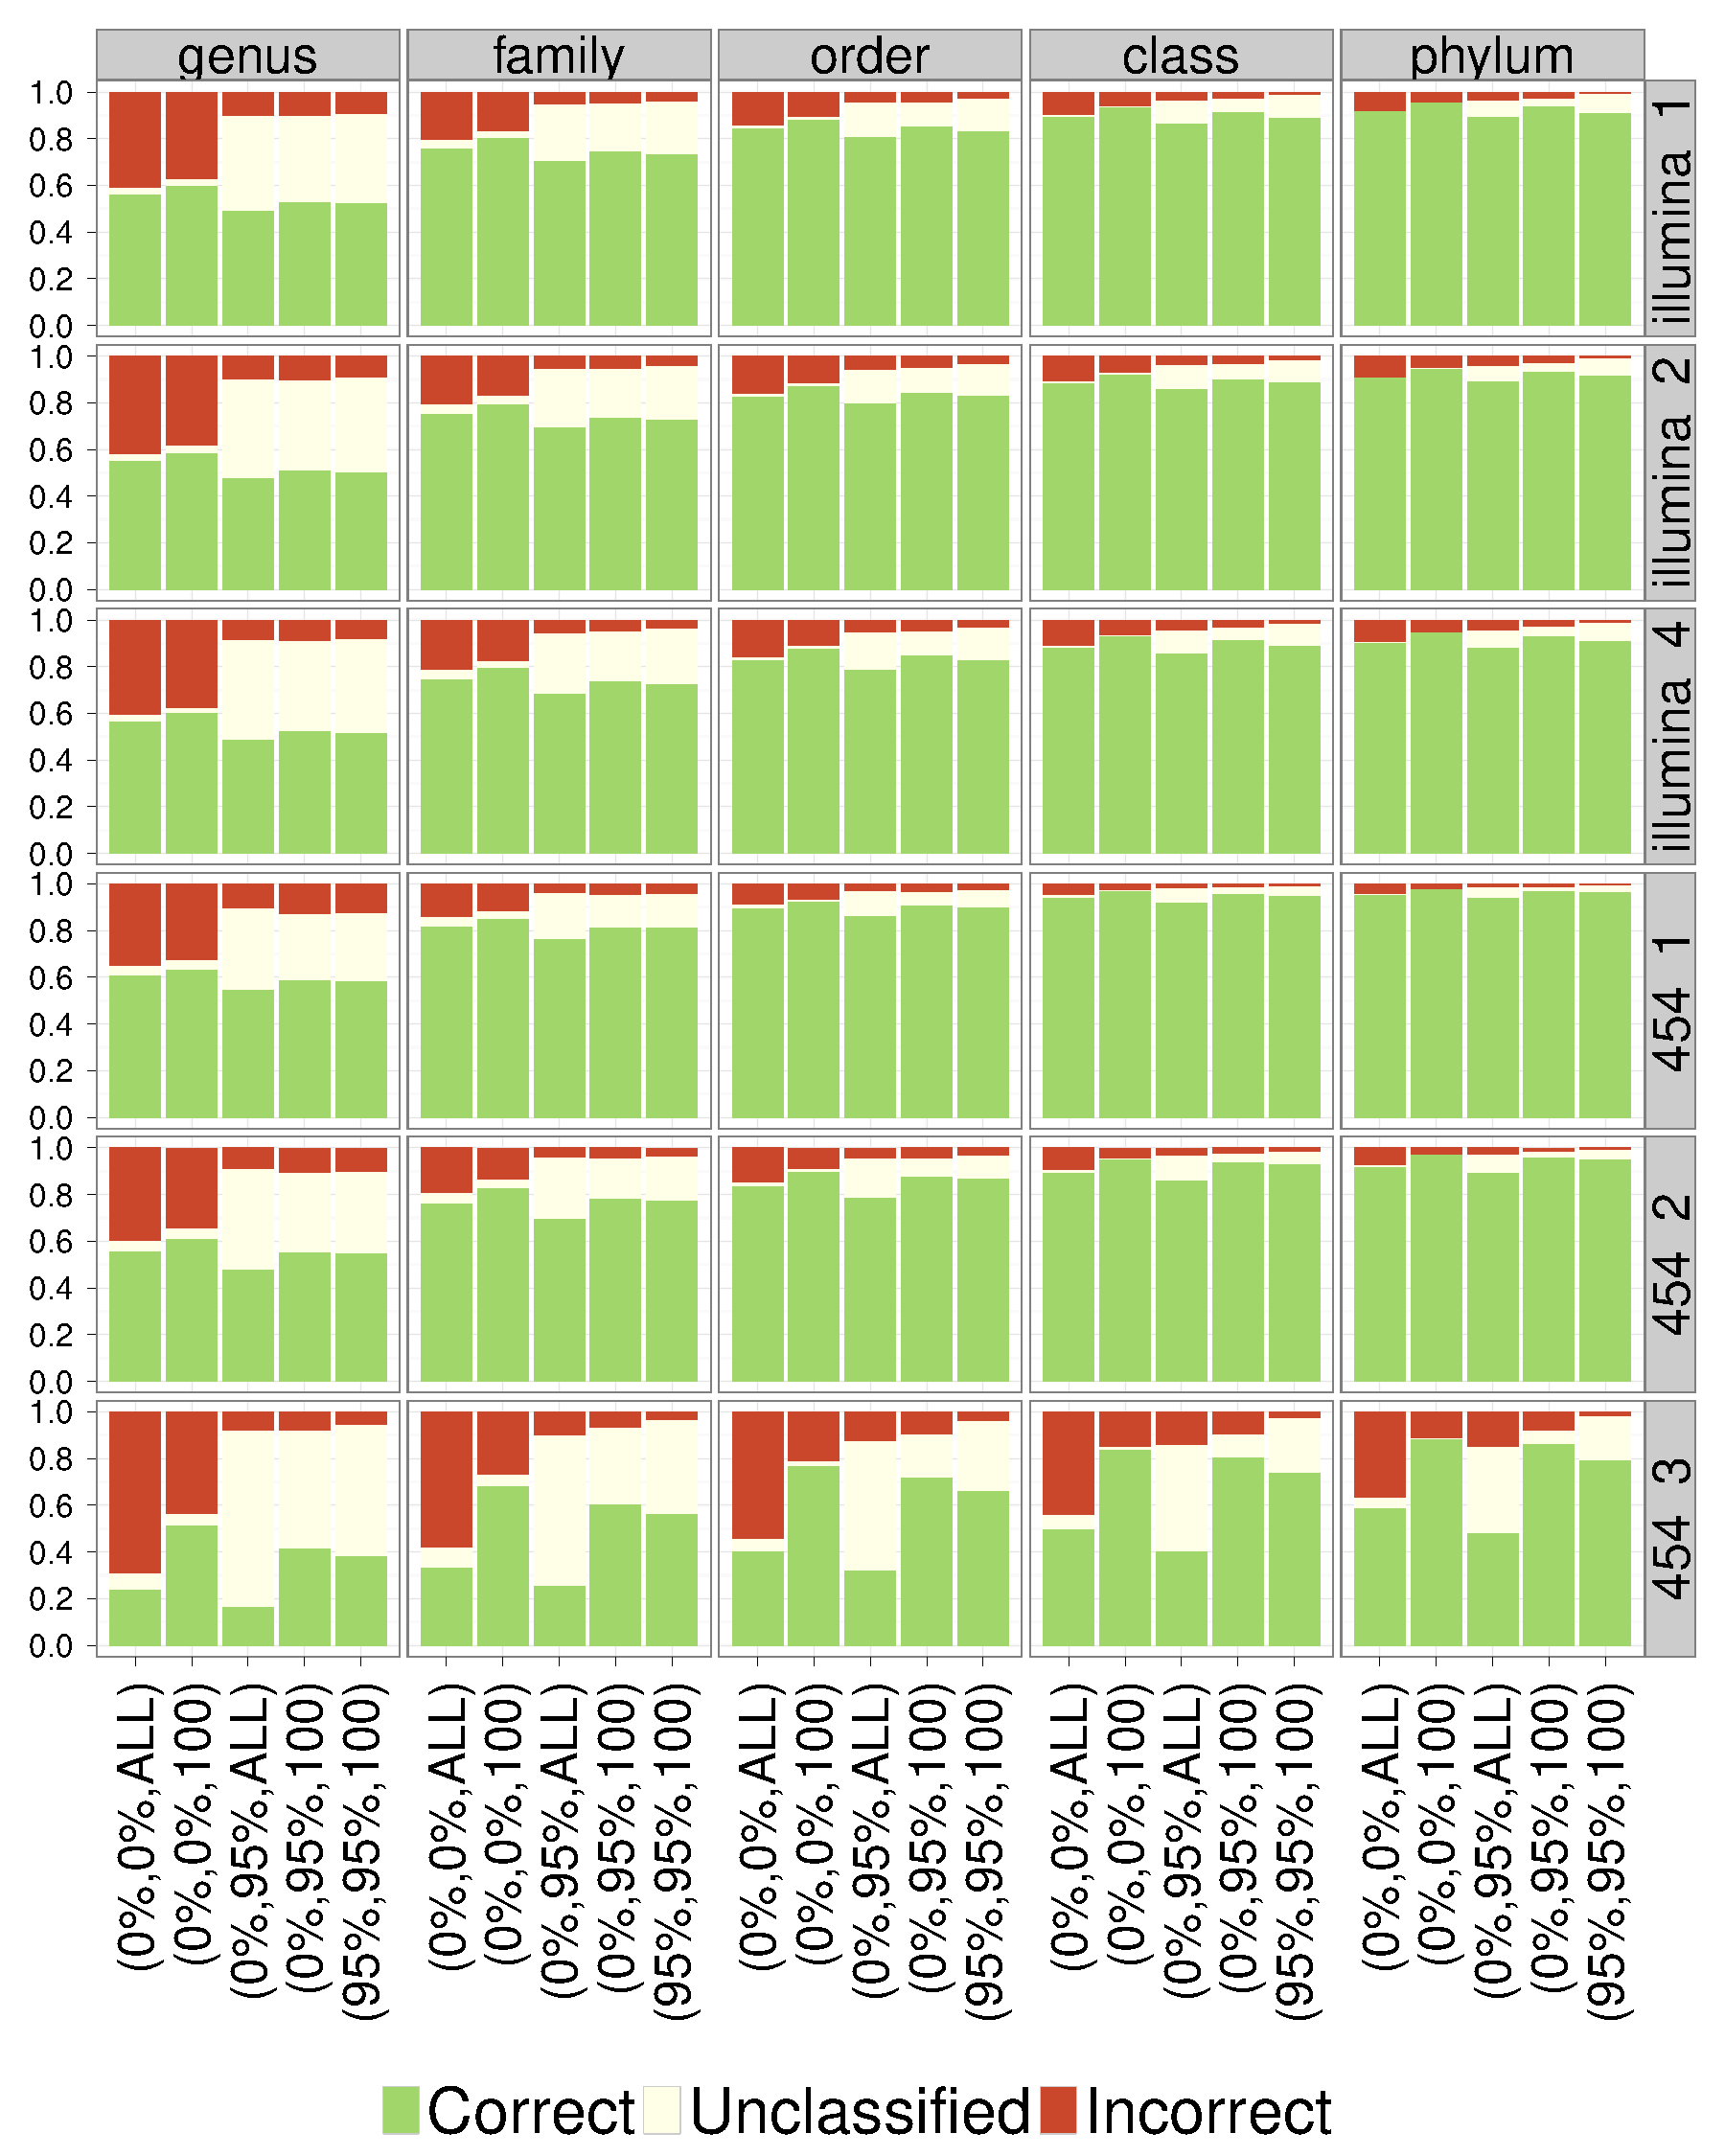
\includegraphics[scale=0.28]{{leaveout/leaveout.higher.species}.pdf}
\end{center}
\caption{\label{tipp:leave_out_tipp_species} Leave-species-out experiment
on the rpsB marker gene, comparing the classification accuracy of different variants of TIPP. 
Each variant is labeled by (X,Y,Z), where X refers to alignment support ($s_a$), Y refers to placement support ($s_p$),
and Z refers to alignment subset size ($m_a$).
Note that SEPP with $m_a=100$
is identical to TIPP(0\%,0\%,100), and that 
HMMER+pplacer is identical to TIPP(0\%,0\%,ALL).}
\end{figure}

\begin{figure}[htpb]
\begin{center}
{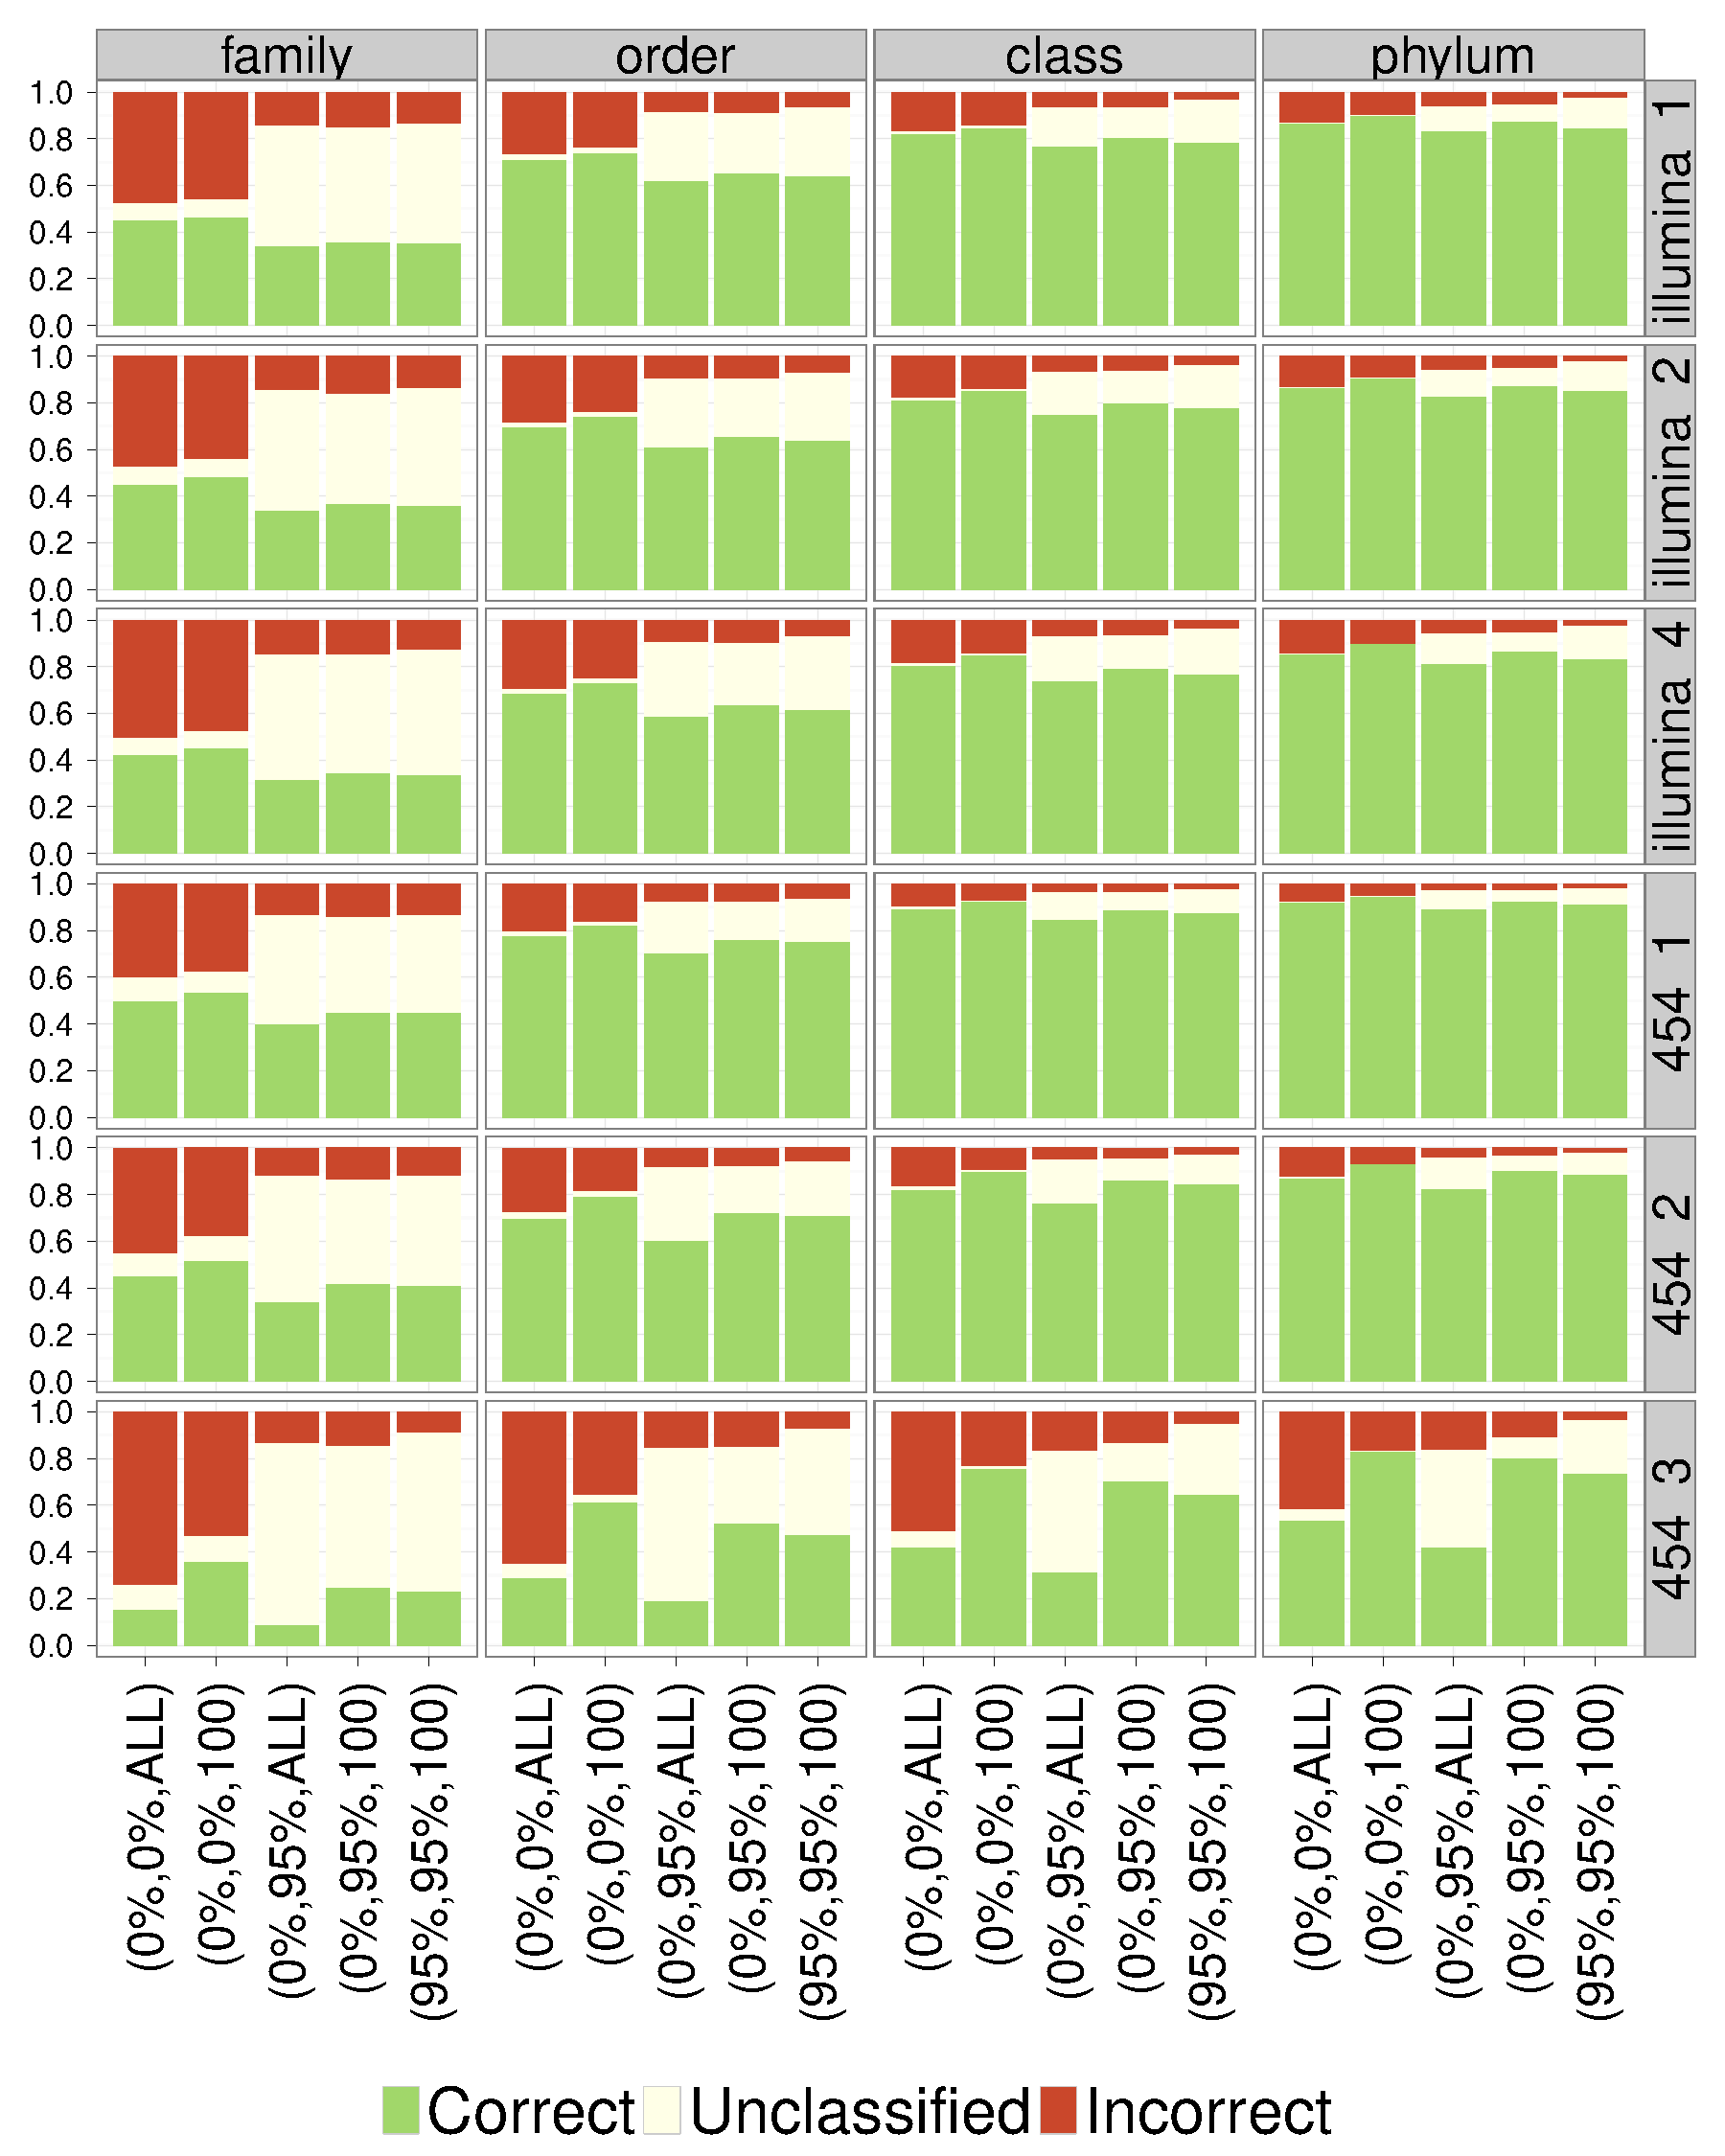
\includegraphics[scale=0.28]{{leaveout/leaveout.higher.genus}.pdf}}
\end{center}
\vspace{-8pt}
\caption{\label{tipp:leave_out_tipp_genus} Leave-genus-out experiment
on the rpsB marker gene,
          comparing the classification accuracy of different variants of TIPP. 
Each variant is labeled by (X,Y,Z), where X refers to alignment support ($s_a$), Y refers to placement support ($s_p$),
and Z refers to alignment subset size ($m_a$). 
%Note that (0\%,0\%,ALL) is equivalent of
%HMMER+pplacer run on the refined taxonomic tree, and (0\%,0\%,100) is equivalent of
%SEPP. (0\%,95\%,ALL) and (0\%,95\%,100) are similar to
%HMMER+pplacer and SEPP, respectively, but consider placement uncertainty. (95\%,95\%,100) corresponds to
%the suggested way of running TIPP (default).
%All results shown here are obtained on rpsB marker gene with both Illumina-like and 454-error like errors.}
%Each column is the classification accuracy
%  for a taxonomic rank and each row the level left out.
%  TIPP($X$\%,$Y$) refers to TIPP run under the default settings with
%  an alignment support and placement support of $X$ and alignment
%  decomposition set size of $Y$.  }
}
\end{figure}

\begin{figure}[htpb]
\begin{center}
{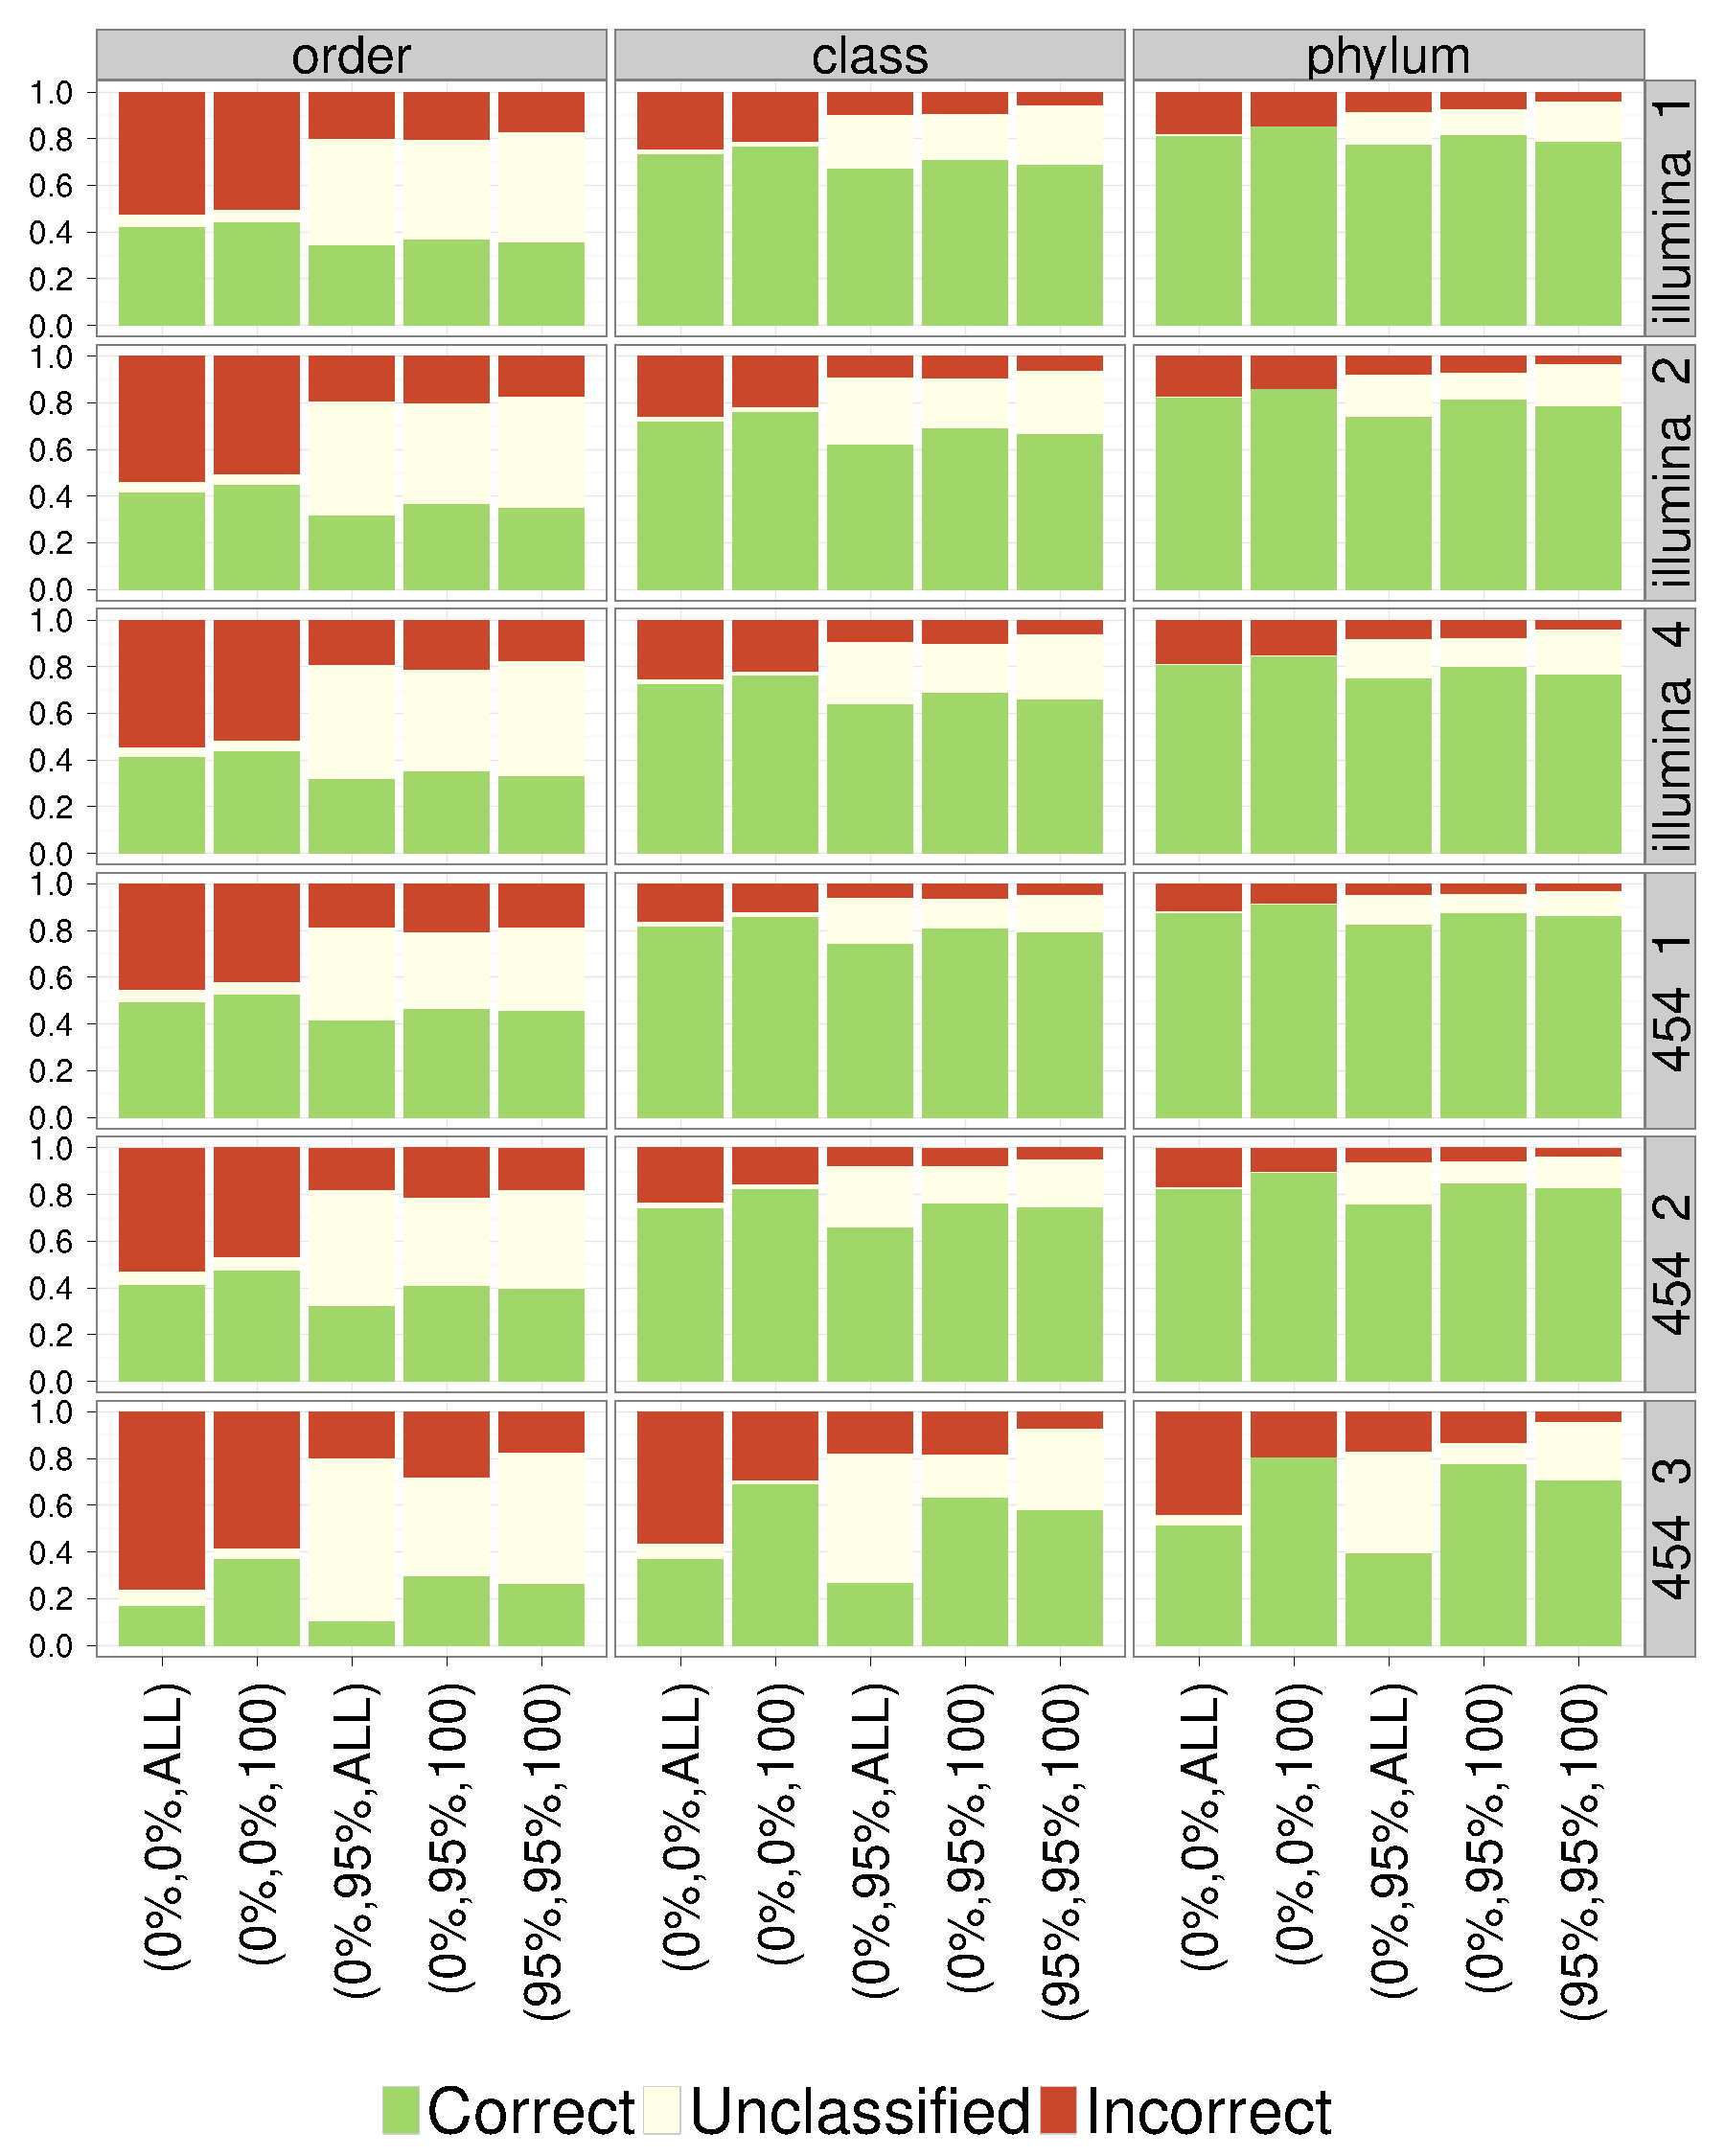
\includegraphics[scale=0.28]{{leaveout/leaveout.higher.family}.pdf}}
\end{center}
\vspace{-8pt}
\caption{\label{tipp:leave_out_tipp_family} Leave-family-out experiment
on the rpsB marker gene,
          comparing the classification accuracy of different variants of TIPP. 
Each variant is labeled by (X,Y,Z), where X refers to alignment support ($s_a$), Y refers to placement support ($s_p$),
and Z refers to alignment subset size ($m_a$). 
%Note that (0\%,0\%,ALL) is equivalent of
%HMMER+pplacer run on the refined taxonomic tree, and (0\%,0\%,100) is equivalent of
%SEPP. (0\%,95\%,ALL) and (0\%,95\%,100) are similar to
%HMMER+pplacer and SEPP, respectively, but consider placement uncertainty. (95\%,95\%,100) corresponds to
%the suggested way of running TIPP (default).
%All results shown here are obtained on rpsB marker gene with both Illumina-like and 454-error like errors.}
%Each column is the classification accuracy
%  for a taxonomic rank and each row the level left out.
%  TIPP($X$\%,$Y$) refers to TIPP run under the default settings with
%  an alignment support and placement support of $X$ and alignment
%  decomposition set size of $Y$.  }
}
\end{figure}
\newpage
% \subsection{Leave-one-out experiments: TIPP versus MetaPhyler}

% In the main paper we showed leave-one-out results comparing TIPP(95\%,95\%,100) and MetaPhyler
% on all marker genes. 
% Here we also show results for TIPP(50\%,50\%,100) in the same experimental setting. 
% Figures \ref{tipp:leave_out_16_bacteria_i} to \ref{tipp:leave_out_30M_i} show results
% similar to Experiment 3 of the main paper, with the addition of TIPP(50\%,50\%,100).

% By design, 
% TIPP(50\%,50\%,100) has higher classification rates than TIPP(95\%,95\%,100), but also has a higher false positive.
% In situations where the reference tree is unlikely to include all bacteria in the community,
% and when revealing new species is important, using more stringent settings is therefore suggested.

% \begin{figure}[htpb]
% \begin{center}
% \subfigure[16S bacteria; Illumina error\label{tipp:leave_out_16_bacteria_i}]{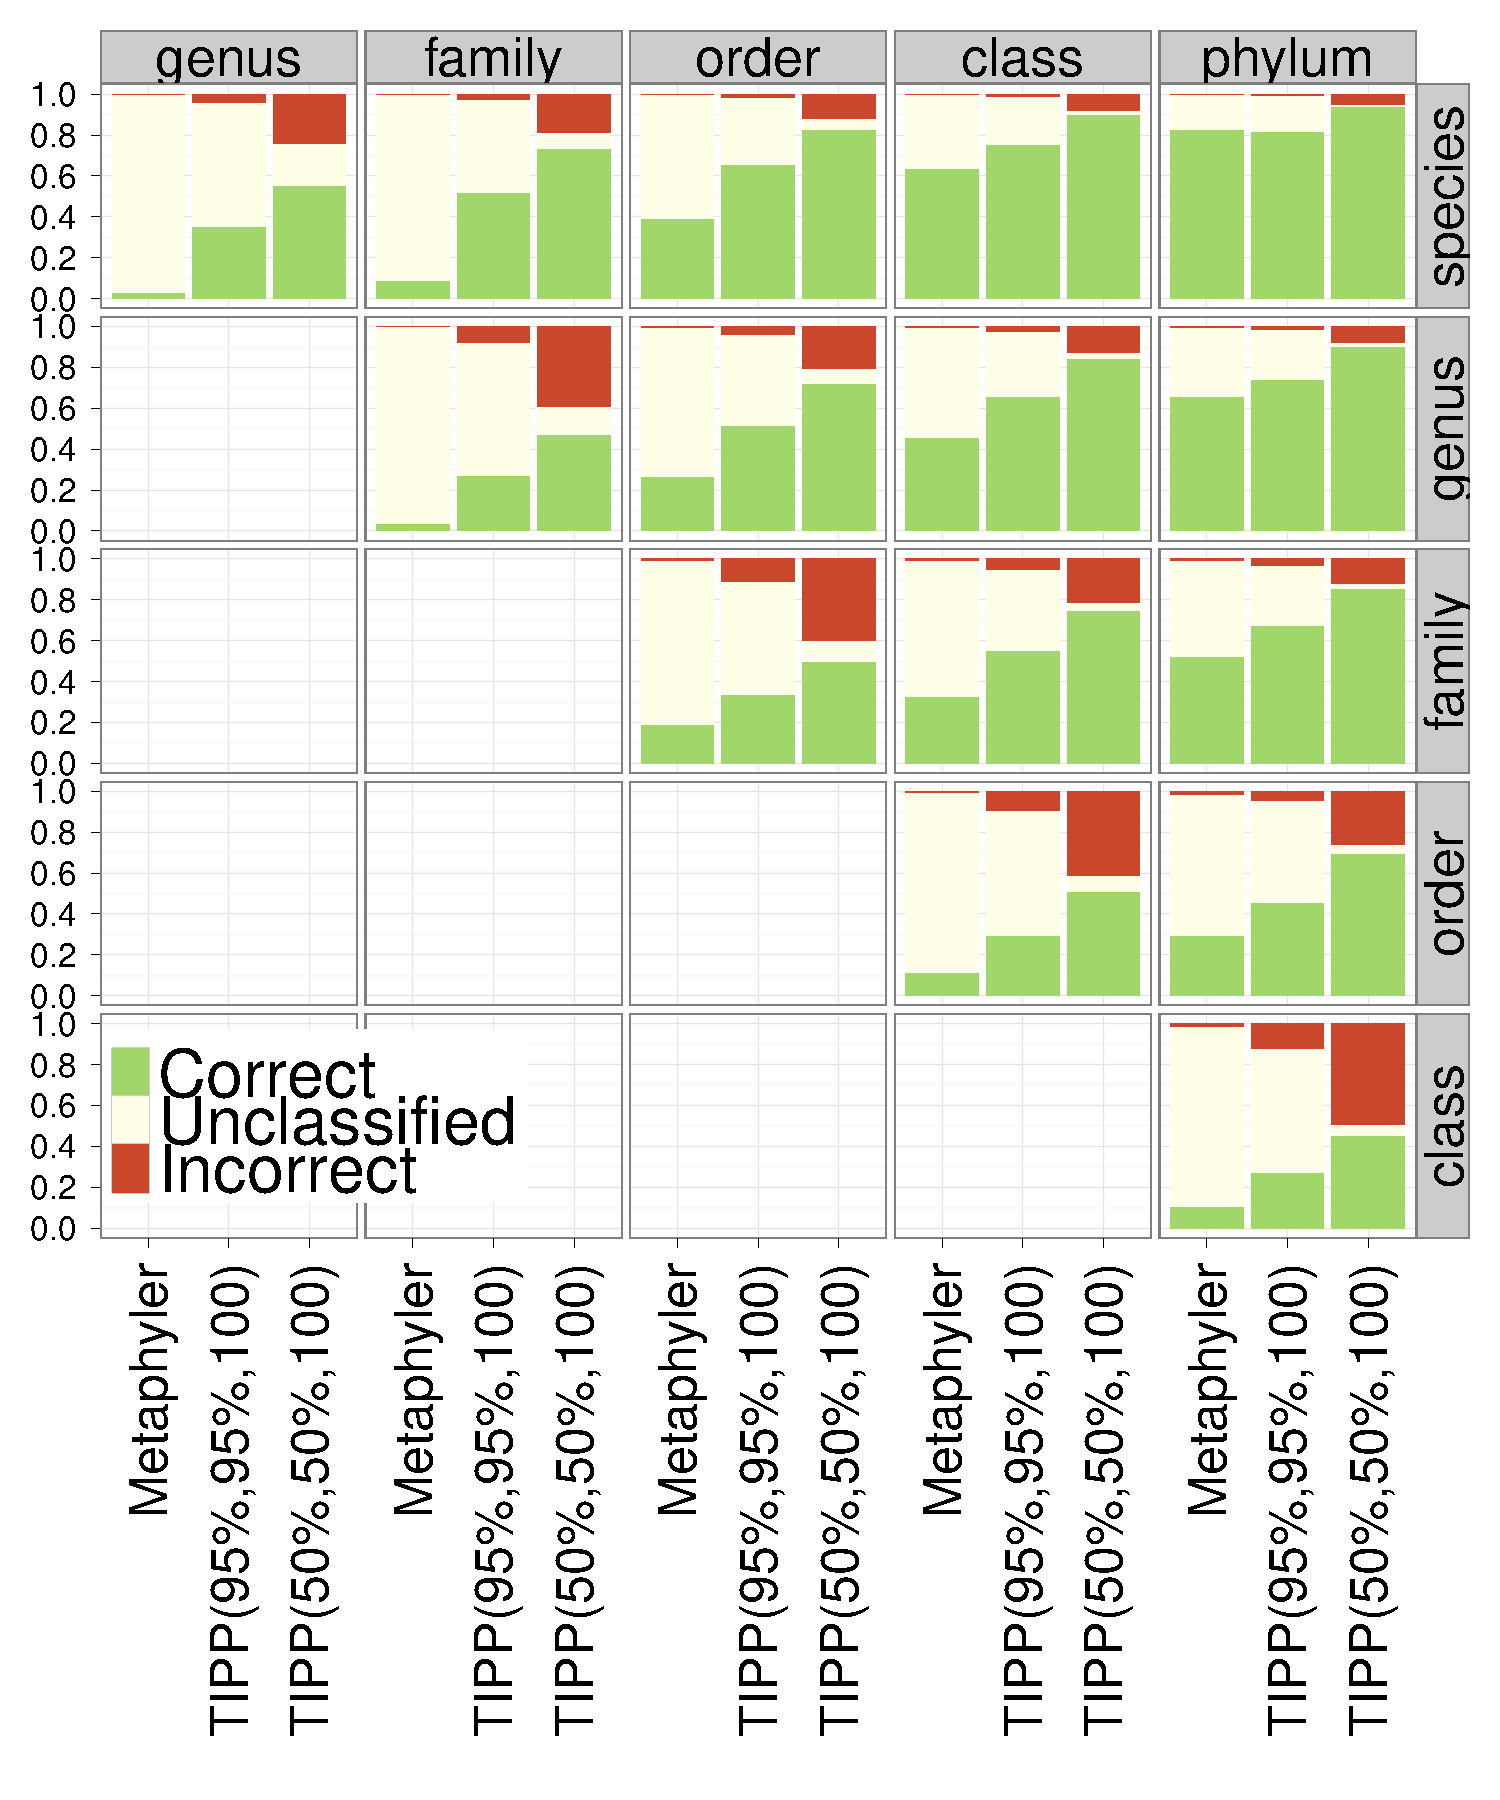
\includegraphics[scale=0.320]{{leaveout/leaveout.illumina.old.16S_bacteria}.pdf}}
% \subfigure[16S bacteria; 454 error\label{tipp:leave_out_16_bacteria_4}]{\includegraphics[scale=0.320]{{leaveout/leaveout.454.old.16S_bacteria}.pdf}}
% \end{center}
% \caption{\label{tipp:leave_out_16-Bacteria} Leave-one-out experiment
          % comparing MetaPhyler
          % to TIPP on the bacterial dataset using the 16S RNA gene,
          % with both Illumina-like and 454-like error models.
	  % For the analyses of the bacterial dataset, due to computational challenges, 
% the placement size is set to 1,000, and the taxonomic tree is used for alignment decomposition.}

% Each column is the classification accuracy
 % for a taxonomic rank and each row the level left out.
 % TIPP($X$\%,$Y$) refers to TIPP run under the default settings with
 % an alignment support and placement support of $X$ and alignment
 % decomposition set size of $Y$.  }
% \end{figure}

% \begin{figure}[htpb]
% \begin{center}
% \subfigure[16S archaea; Illumina error\label{tipp:leave_out_16_archaea_i}]{\includegraphics[scale=0.32]{{leaveout/leaveout.illumina.old.16S_archaea}.pdf}}
% \subfigure[16S archaea; 454 error\label{tipp:leave_out_16_archaea_4}]{\includegraphics[scale=0.32]{{leaveout/leaveout.454.old.16S_archaea}.pdf}}
% \end{center}
% \caption{\label{tipp:leave_out_16-Archaea} Leave-one-out experiment
          % comparing MetaPhyler
          % to TIPP on the archae dataset using the 16S  gene,
          % with both Illumina-like and 454-like error models.
     % }

% Each column is the classification accuracy
 % for a taxonomic rank and each row the level left out.
 % TIPP($X$\%,$Y$) refers to TIPP run under the default settings with
 % an alignment support and placement support of $X$ and alignment
 % decomposition set size of $Y$.  }
% \end{figure}

% \begin{figure}[htpb]
% \begin{center}

% \subfigure[Illumina error model\label{tipp:leave_out_30M_i}]{\includegraphics[scale=0.32]{{leaveout/leaveout.illumina.old}.pdf}}
% \subfigure[454 error model\label{tipp:leave_out_30M_4}]{\includegraphics[scale=0.32]{{leaveout/leaveout.454.old}.pdf}}
% \end{center}
% \caption{\label{tipp:leave_out_30M} Leave-one-out experiment
          % comparing the classification accuracy for MetaPhyler
          % versus TIPP on 30 marker genes with both Illumina-like and 454-error like errors.  
% }
% Each column is the classification accuracy
 % for a taxonomic rank and each row the level left out.
 % TIPP($X$\%,$Y$) refers to TIPP run under the default settings with
 % an alignment support and placement support of $X$ and alignment
 % decomposition set size of $Y$.  }
% \end{figure}

\newpage
\subsection{TIPP Boosting of EPA versus pplacer}\label{tipp:tipp.epa.pplacer.sec}
TIPP requires an external placement tool for its placement step. 
While the initial submission only used pplacer, the current
current implementation of TIPP
can use both pplacer and EPA. The results in the main
paper are based on using pplacer internally, and here we 
show results on using EPA inside TIPP, compared 
to using pplacer inside TIPP, in a leave-species-out experiment on the rpsB marker gene. 
We observe that in this experiment, TIPP using pplacer and EPA 
are almost identical
(Figure \ref{tipp:tipp.epa.pplacer});
the differences in recall between 
the two techniques are statistically
significant only when placing at the class or phylum level and
the differences between precision is never statistically significant (Table \ref{tipp:tipp.epa.pplacer.tab}). 

\begin{figure}[htpb]
\begin{center}
\includegraphics[scale=0.32]{{leaveout/leaveout.epa_pplacer.species}.pdf}
\end{center}
\caption{\label{tipp:tipp.epa.pplacer} Leave-one-out experiment
          comparing the classification accuracy for TIPP with default settings when it uses EPA or pplacer internally
for the placement step. Results are for a leave-species-out experiment on the rpsB marker 
gene with Illumina-like errors. Differences in recall are
statistically significant at the class and phylum levels, but not
below the class level.   }
\end{figure}

\begin{table}[hptb]
\caption{\label{tipp:tipp.epa.pplacer.tab} Precision and recall of TIPP when it uses EPA or pplacer internally
for the placement step. The table shows the difference between precision and recall 
values of the two techniques (delta) and p-value of a statistical test showing
whether the differences are statistically significant according to the Pearson's chi-square contingency table test (as implemented in R~\cite{R}).
Positive values mean TIPP with pplacer was better than TIPP with EPA.
Results are for a leave-species-out experiment on the rpsB marker 
gene with Illumina-like errors. 
Differences in recall are
statistically significant at the class and phylum levels, but not
below the class level. In all other cases differences are not statistically significant. }
\begin{center}
\begin{tabular}{|l|c|c|c|c|c|} \hline
&\multicolumn{1}{|c|}{genus}&\multicolumn{1}{c|}{family}&\multicolumn{1}{c|}{order}&\multicolumn{1}{c|}{class}&\multicolumn{1}{c|}{phylum}\\ \hline
{\bf Recall} &&&&&\\
~Delta &~0.006&~0.012&~0.013&{\bf ~0.013}&{\bf ~0.011}\\ 
~p-value &0.5617&0.1975&0.0763&{\bf 0.0244}&{\bf 0.0165}\\ \hline
{\bf Precision} &&&&&\\
~Delta &~0.000&-0.001&~0.002&~0.003&~0.001\\ 
~p-value & 0.9960&0.8662&0.6282&0.2412&0.4704\\ 
\hline
\end{tabular}
\end{center}
\end{table}

\newpage
\subsection{Non-leave-one-out Parameter Exploration Study}\label{supp:tipp_non_leaveout_variants}
In this section we report on non-leave-one-out experiments performed on the rpsB marker gene
in order to further understand the impact of parameter settings on the accuracy of TIPP. Note that results from
these non-leave-one-out experiments should be interpreted in conjunction with
leave-one-out results presented earlier. The impact of parameter settings could
be quite different between non-leave-one-out and leave-one-out results, hence caution is required in interpreting the results. 
In general, changing TIPP parameters show a higher impact on classification accuracy in leave-one-out experiments. 
In non-leave-one-out experiments, the impact of
changes to the TIPP parameters is often most observable at the highest error model conditions.

\paragraph{Placement Support.}  Placement support has a large impact on the overall classification accuracy (Fig.~\ref{tipp:placement_support}). For both types of sequencing error, the largest of varying placement support is at the species level; increasing the placement support results in fewer incorrect and correct classifications.  The impact of placement support is most visible on 454 models with higher rates of error.  A sizeable portion of the false positives can be removed by using higher placement support values.

\begin{figure}[htpb]
\begin{center}
\begin{subfigure}[htpb]{\textwidth}
\includegraphics[scale=0.300]{{higher_error/higher_error_illumina_placement_1_5_13}.pdf}\\
\caption[]{Illumina-like fragments}
\end{subfigure}
\end{center}
\begin{center}
\begin{subfigure}[htpb]{\textwidth}
\includegraphics[scale=0.300]{{higher_error/higher_error_454_placement_1_5_13}.pdf}\\
\caption[]{454-like fragments}
\end{subfigure}
\end{center}
\caption[Varying placement support.]{\label{tipp:placement_support}Non-leave-one-out experiments showing the impact of changing placement support on the classification accuracy for fragments simulated from the rpsB gene with (a) Illumina-like errors and (b) 454-error like errors.  Each column is the classification accuracy for a taxonomic rank and each row is the error model used.  TIPP($X$\%,$Y$\%,$Z$) refers to TIPP run under the default settings with an alignment support of $X$, placement support of $Y$, and maximum alignment decomposition subset size of $Z$.}
\end{figure}

\paragraph{Alignment Support.}  Figures~\ref{tipp:alignment_support_50} and ~\ref{tipp:alignment_support_95} show the result of fixing the placement support to be 50\% or 95\%, and changing the alignment support threshold.  Increasing the alignment support has a slight impact on the overall classification accuracy for the Illumina-type errors.  The differences between the percentage of fragments classified at all levels for 0\% alignment support and 95\% alignment support is less than 5 percentage points. 
For the 454-type errors, the impact of alignment support is only noticeable for the higher error model conditions.  
Note that leave-one-out results were impacted more by varying alignment support.

\begin{figure}[htpb]
\begin{center}
\begin{subfigure}[htpb]{\textwidth}
\includegraphics[scale=0.300]{{higher_error/higher_error_illumina_alignment_50_1_5_13}}\\
\caption[]{Illumina-like fragments}
\end{subfigure}
\end{center}
\begin{center}
\begin{subfigure}[htpb]{\textwidth}
\includegraphics[scale=0.300]{{higher_error/higher_error_454_alignment_50_1_5_13}}\\
\caption[]{454-like fragments}
\end{subfigure}
\end{center}
\caption[Varying alignment support with placement support of 50\%.]{\label{tipp:alignment_support_50}Non-leave-one-out experiments showing the impact of changing alignment support while fixing the placement support to be 50\% on the classification accuracy for fragments simulated under the (a) Illumina error model and (b) 454 error model for the rpsB marker gene.  Each column is the classification accuracy for a taxonomic rank and each row is the error model used.  TIPP($X$\%,$Y$\%,$Z$) refers to TIPP run under the default settings with an alignment support of $X$, placement support of $Y$, and maximum alignment decomposition subset size of $Z$.}
\end{figure}

\begin{figure}[htpb]
\begin{center}
\begin{subfigure}[htpb]{\textwidth}
\includegraphics[scale=0.300]{{higher_error/higher_error_illumina_alignment_95_1_5_13}}\\
\caption[]{Illumina-like fragments}
\end{subfigure}
\end{center}
\begin{center}
\begin{subfigure}[htpb]{\textwidth}
\includegraphics[scale=0.300]{{higher_error/higher_error_454_alignment_95_1_5_13}}\\
\caption[]{454-like fragments}
\end{subfigure}
\end{center}
\caption[Varying alignment support with placement support of 95\%.]{\label{tipp:alignment_support_95}Non-leave-one-out experiments showing the impact of changing alignment support while fixing the placement support to be 95\% on the classification accuracy for fragments simulated under the (a) Illumina error model and (b) 454 error model for the rpsB marker gene.  Each column is the classification accuracy for a taxonomic rank and each row is the error model used.  TIPP($X$\%,$Y$\%,$Z$) refers to TIPP run under the default settings with an alignment support of $X$, placement support of $Y$, and maximum alignment decomposition subset size of $Z$.}
\end{figure}

\paragraph{Alignment Support and Placement Support.} Figure~\ref{tipp:general_support} shows the result of changing alignment support and placement support together.  TIPP(0\%,0\%,100) tends to over-classify, resulting in the largest percentage of  incorrect classifications.  Both TIPP(25\%,25\%,100) and TIPP(50\%,50\%,100) result in a drop of correct classifications at the species level, but, at the same time, a larger drop in incorrect classifications at the species level.  The drop in correct classifications is not noticeable for the higher taxonomic levels on the error models with low rates of error.   TIPP(95\%,95\%,100) has a large decrease of correct classifications at the species level, but also has the fewest incorrect classifications at all levels for all error models; nearly all the error for the lower error model conditions are eliminated.
%From result, propose two versions of TIPP, TIPP liberal (TIPP(50\%,50\%)) and conservative version (TIPP(95\%,95\%)).  
%\textbf{Need to justify why 50\% and why 95\%}
%\textbf{ADD ROC CURVES FOR RESULTS}

\begin{figure}[htpb]
\begin{center}
\begin{subfigure}[htpb]{\textwidth}
\includegraphics[scale=0.300]{{higher_error/higher_error_illumina_best_1_5_13}}\\
\caption[]{Illumina-like fragments}
\end{subfigure}
\end{center}
\begin{center}
\begin{subfigure}[htpb]{\textwidth}
\includegraphics[scale=0.300]{{higher_error/higher_error_454_best_1_5_13}}\\
\caption[]{454-like fragments}
\end{subfigure}
\end{center}
\caption[Varying alignment support and placement support.]{\label{tipp:general_support}Non-leave-one-out experiments showing the impact of changing both alignment support and placement support on classification accuracy for fragments simulated from the rpsB gene with (a) Illumina-like errors and (b) 454-error like errors.  Each column is the classification accuracy for a taxonomic rank and each row is the error model used.  TIPP($X$\%,$Y$\%,$Z$) refers to TIPP run under the default settings with an alignment support of $X$, placement support of $Y$, and maximum alignment decomposition subset size of $Z$.
}
\end{figure}


\paragraph{Impact of maximum alignment subset size. }
We found that using smaller alignment subset sizes tends to improve accuracy, 
especially at the species level,
but also increases the running time as there are more alignment subsets to analyze:
the wall clock time to classify 200,000 fragments from the rpsB gene ranged from 2.1 hours  for TIPP(95\%,95\%,ALL) to 3.6 hours for TIPP-default (TIPP(95\%,95\%,100)) (each run with 4 CPUs).  The number of sequences in the reference alignment also impacts the running time for the TIPP(95\%,95\%,ALL) method, but this scales (at most) linearly with the number of sequences. The running time shown for the rpsB gene is a good case study, since the reference alignment has 1463 sequences and is one of the larger datasets  in this study.

Figure ~\ref{tipp:alignment_size_95} shows the impact of changing the alignment decomposition size on TIPP(95\%,95\%).  The result shows that, in general, decreasing the alignment decomposition size increases the percentage of correctly classified fragments, as well as decreases the percentage of incorrectly classified fragments.  
In other words, smaller alignment subsets produce more accurate placements.
However, using smaller alignment decomposition sizes results in an increase in running time.

\begin{figure}[htpb]
\begin{center}
%\subfigure[Illumina-like fragments]{\includegraphics[scale=0.300]{higher_error/higher_error_illumina_size_95_1_5_13}}\\
\end{center}
\begin{center}
%\subfigure[454-like fragments]{\includegraphics[scale=0.300]{higher_error/higher_error_454_size_95_1_5_13}}\\
\end{center}
\caption[Varying decomposition size for TIPP(95\%).]{\label{tipp:alignment_size_95}Non-leave-one-out experiments showing the impact of changing the size of the alignment decomposition for TIPP(95\%) for fragments simulated from the rpsB gene with (a) Illumina-like errors and (b) 454-error like errors.  Each column is the classification accuracy for a taxonomic rank and each row is the error model used. TIPP($X$\%,$Y$) refers to TIPP run under the default settings with an alignment support and placement support of $X$ and a maximum alignment decomposition subset size of $Y$.
}
\end{figure}


\subsection{ROC Curves}
Here we explore the impact of change in support threshold for
alignment subsets of size $10$ in a non-leave-one-out experiment on
the rpsB marker gene (one of the hardest in the dataset), as
alignment and placement support thresholds are increased progressively.

The ROC curves shown in Figure \ref{tipp:roc_curve_full} show
that the impact of the support thresholds
is very visible at the species level, very reduced at the genus level, and then largely
eliminated at the family level and above.  
The curves for the species-level classification show that there is a tight
 relationship between the precision and recall as the
support varies between 0\% to 50\%, but that
the gain in precision
moving from 50\% support to 95\% support is significantly smaller than
the loss in recall (1-2\% gain in precision but 6-10\% drop in
recall).  

\begin{figure}[htpb]
\begin{center}
%\subfigure[Results on rpsB data, non-leave-one-out]{\includegraphics[scale=0.250]{higher_error/roc_higher_error_illumina_all_1_5_12}}\\
\includegraphics[scale=0.40]{higher_error/roc_higher_error_illumina_all_1_5_12}
\end{center}
%\begin{center}
%\subfigure[454-like fragments]{\includegraphics[scale=0.300]{higher_error/roc_higher_error_454_all_1_5_12}}\\
%\end{center}
\caption[ROC curve for TIPP on rpsB data]{\label{tipp:roc_curve_full}ROC curve showing the
  impact of the different support thresholds on precision and recall
  for species-level to family-level classification of
  fragments simulated from the rpsB marker genes in a
  non-leave-one-out experiment under the Illumina-error models. 
Note TIPP(0\%,0\%,10) is the same as 
SEPP with alignment subset size $m_a=10$.
%TIPP($X$\%,$Y$) refers to TIPP run under the
%  default settings with an alignment and placement support of $X$ and
%  an alignment decomposition subset size of $Y$.  Each column is the
%  ROC curve for a taxonomic rank and each row is the error model
%  used.
}
\end{figure}

\newpage
\subsection{Leave-one-out TIPP versus Metaphyler}  
Next, to compare TIPP and MetaPhyler, we performed a
leave-one-out study  on the 
30 marker genes used in the original MetaPhyler paper and
on the 16S gene.
%Figures \ref{tipp:leave_out_16} and \ref{tipp:leave_out_30M} 
Here we show results for the default setting for TIPP (i.e., TIPP(95\%,95\%,100)).

\subsubsection{Leave-one-out 30 marker genes}
Figures~\ref{tipp:leave_out_30M} shows the result for the leave-one-out
experiments for the 30 marker genes. 
TIPP has higher recall on these data than
MetaPhyler, and the differences are substantial and
statistically significant (p-values $\ll 10^{-5}$).
The comparison with respect to precision
% (i.e., false classifications)
is very interesting:
while TIPP generally had better precision in about two-thirds of
the cases,
 MetaPhyler had better precision one third of the time (except in one case, 
differences are statistically significant, p-value $\ll10^{-5}$; see Section \ref{supp:leave_one_out_tipp_meta_table}).
Furthermore, the relative performance depended on the
taxonomic level, so that
MetaPhyler had better precision
at the lower taxonomic levels,
and TIPP had better precision at the higher
taxonomic levels.

\subsubsection{Leave-one-out 16S RNA gene}
Figures~\ref{tipp:leave_out_16}
show the result for the leave-one-out experiments for the 16S rRNA
gene.  TIPP classifies more fragments correctly
than MetaPhyler on these data, especially at the lower taxonomic levels.
MetaPhyler generally had very low false classification
rates.  TIPP's false classification
rates were generally low, except 
when a taxonomic clade at the family or higher level is removed 
and classification is tested at the next taxonomic level.
A detailed analysis of these cases revealed that
the false classifications were mostly due
to peculiarities in the taxonomy,
potentially due to sparse taxonomic 
sampling.  

For example, in the 16S Archaea taxonomy, the Halobacteria class has exactly one family.  Therefore, the leave-one-family-out experiment results in an imbalanced taxonomy with no sequences from the Halobacteria class present in the taxonomy, and the nearest relatives are at the phylum level.  As a result, it is impossible to correctly classify the fragments at the order or class level.  Because TIPP tends to classify fragments if it can do so with some confidence, this results in a higher false classification rate (see Section~\ref{supp:archaea} for more detailed discussion).  

MetaPhyler generally had better precision than
TIPP, but at a substantial cost in recall, especially
at the lower taxonomic levels.
For example, in the leave-out-species
experiments for the 454 bacterial 16S rRNA fragments, MetaPhyler
classified only 15\% correctly at the genus level, and TIPP
classified 69\% correctly.  On the other hand, the false
classification rate for MetaPhyler was quite low, varying from
less than 1\% to 3\%, while the false classification rate for
TIPP was somewhat higher.  On the bacterial 16S rRNA gene
set, the false classification rate for TIPP was quite low
(with the exception of the phylum level in the leave-one-class-out
experiment). On the archaeal 16S rRNA genes, 
TIPP generally had low false classification rates, but
there were a few cases
where TIPP had high false classification rates.

\begin{figure}[htpb]
\begin{center}
%\mbox{
%\subfigure[Illumina error model\label{tipp:leave_out_30M_i}]{\includegraphics[scale=0.3]{{leaveout/leaveout.illumina}.pdf}}
\hspace{-14pt}
%\subfigure[454 error model\label{tipp:leave_out_30M_4}]{\includegraphics[scale=0.3]{{leaveout/leaveout.454}.pdf}}}
\end{center}

\caption{\label{tipp:leave_out_30M} Leave-one-out experiment
          comparing the classification accuracy for MetaPhyler
          versus TIPP-default 
(i.e.,  TIPP-default refers to TIPP(95\%,95\%,100))
on the 30 marker genes.
%with both Illumina-like and 454-error like errors.  
}
%Each column is the classification accuracy
%  for a taxonomic rank and each row the level left out.
%  TIPP($X$\%,$Y$) refers to TIPP run under the default settings with
%  an alignment support and placement support of $X$ and alignment
%  decomposition set size of $Y$.  }
\end{figure}

\begin{figure*}[htpb]
\begin{center}

%\subfigure[16S bacteria; Illumina error\label{tipp:leave_out_16_bacteria_i}]{\includegraphics[scale=0.300]{{leaveout/leaveout.illumina.16S_bacteria}.pdf}}
\hspace{-14pt}
%\subfigure[16S bacteria; 454 error\label{tipp:leave_out_16_bacteria_4}]{\includegraphics[scale=0.300]{{leaveout/leaveout.454.16S_bacteria}.pdf}}
%\subfigure[16S archaea; Illumina error\label{tipp:leave_out_16_archaea_i}]{\includegraphics[scale=0.30]{{leaveout/leaveout.illumina.16S_archaea}.pdf}}
\hspace{-14pt}
%\subfigure[16S archaea; 454 error\label{tipp:leave_out_16_archaea_4}]{\includegraphics[scale=0.30]{{leaveout/leaveout.454.16S_archaea}.pdf}}

\end{center}
\caption{\label{tipp:leave_out_16} Leave-one-out experiment
          comparing MetaPhyler
          to TIPP on the 16S bacteria (a-b) and 16S archaea (c-d) datasets,
          with both Illumina-like and 454-like error models.
    TIPP-def refers to TIPP run
          under the default settings (i.e. TIPP(95\%,95\%,100)).
          TIPP-large is similar to TIPP-def, except placement size is set to 1,000, and the taxonomic tree is used for alignment decomposition.}
\end{figure*}

\subsection{16S RNA on archaea, leave-one-out experiments; effects of Halobacteria}\label{supp:archaea}
In this section we discuss the particularly high false 
classification rates for the leave-family-out 
and leave-order-out experiments for 16S RNA on archaea ().  
We find that the majority of the false classifications are caused by the Halobacteria class,
and  37\% of all fragments from the 16S RNA on Archaea dataset
belong to this class.  
For the leave-family-out experiment, 
the total numbers of incorrect classifications for 
TIPP(95\%,95\%,100) at the order level and class level 
were 13,651 and 18,456, respectively.  
Of those incorrect classifications, 9,223 of the 13,651 (68\%) and 
15,187 of the 18,456 (82\%) belong to fragments from this class.

Figure~\ref{tipp:taxonomy} highlights the reason for the large number of incorrect classifications.  Most normal OTUs have more than direct child OTU, i.e. phyla typically have more than one class, and classes typically have more than one order.  The Halobacteria class has only one order, and that order has only one family.  Thus, removing either the family or the order prunes the entire class from the taxonomy.  This makes it impossible to correctly classify fragments at either the order level or the class level.  Note that this phenomenon is not unique to Halobacteria:  any OTU that has exactly one direct child OTU will 
be removed completely when the child OTU is omitted in the 
leave-one-out experiment.  
This is most notable in Halobacteria because of the large number of fragments belonging to this class.

Figure~\ref{tipp:remove_class} shows the result of omitting fragments from this class from the leave-family-out and leave-order-out experiments.  When Halobacteria is omitted, the incorrect classification rate drops and is in line with the incorrect classification rates for the 16S experiments.
\begin{figure}[htpb]
\begin{center}
{\includegraphics[scale=0.35]{{leaveout/taxonomy2}.pdf}}
\end{center}
\vspace{-8pt}
\caption{\label{tipp:taxonomy} Taxonomy for Halobacteria class for the 16S RNA gene.
}
\end{figure}

\begin{figure}[htpb]
\begin{center}
%\subfigure[Illumina-like fragments]{\includegraphics[scale=0.300]{leaveout/{leaveout.illumina.no_110.16S_archaea}.pdf}}\\
\end{center}
\begin{center}
%\subfigure[454-like fragments]{\includegraphics[scale=0.300]{leaveout/{leaveout.454.no_110.16S_archaea}.pdf}}\\
\end{center}
\caption[Removing Halobacteria class from leave-family-out and leave-order-out experiments.]{\label{tipp:remove_class}Removing Halobacteria class from leave-family-out and leave-order-out experiments for 16S RNA archaea gene for fragments simulated with (a) Illumina-like errors and (b) 454-error like errors.  Each column is the classification accuracy for a taxonomic rank and each row is level being omitted.}
\end{figure}
\clearpage
\subsection{Experiment 2: Abundance profiling experiments}
We show the impact of alignment and placement support on abundance 
profiling (Fig.~~\ref{tipp:profile_short_tipp_compare} and 
\ref{tipp:profile_long_tipp_compare}).  
Although results depended on the particular dataset, 
the following trends can be observed.
On the short fragment datasets,
on average
 using the 0\% threshold improved average abundance profiles 
at the lower taxonomic levels
and was neutral at the phylum level.
On the long fragment datasets, the change in threshold had
essentially no impact.  This result lead us to select TIPP(0\%,0\%,100) for abundance profiling.


\begin{figure*}[htpb]
\begin{center}
{\includegraphics[scale=0.7]{{profiles/profiles.shortsequences.fp.tipp}.pdf}}
\end{center}
\caption{\label{tipp:profile_short_tipp_compare} Abundance profiling results comparing different TIPP methods on short fragments.  The RMSE has been normalized by TIPP(0\%,0\%,100)'s RMSE.  }
\end{figure*}


\begin{figure*}[htpb]
\begin{center}
{\includegraphics[scale=0.7]{{profiles/profiles.longsequences.fp.tipp}.pdf}}
\end{center}
\caption{\label{tipp:profile_long_tipp_compare} Abundance profiling results comparing different TIPP methods on long fragments.  The RMSE has been normalized by TIPP(0\%,0\%,100)'s RMSE.  }
\end{figure*}

In the main paper, we compare TIPP-default against other abundance profiling methods.  The tabular results for the figures are shown in Tables~\ref{tipp:table_abundance_short} and \ref{tipp:table_abundance_long}.

%Table has been updated with the new scoring metric
\begin{table}[hptb]
\caption[Normalized $RMSE$ for different methods on short fragment datasets.]{\label{tipp:table_abundance_short}
The $RMSE$ for different methods on the short fragment datasets, normalized by TIPP(0\%,0\%,100)'s $RMSE$ for each model condition and each taxonomic rank.  Thus methods with $RMSE>1$ have worse performance than TIPP, and methods with $RMSE<1$ have better performance than TIPP.  Note that PhymmBL does not output species level classification.   \textbf{fix size!}}
\begin{center}
\scalebox{0.7}{
\begin{tabular}{|l|r|r|r|r|r|r|}
\hline
Dataset&Species&Genus&Family&Order&Class&Phylum\\
{\bf FACs HC Illumina}&&&&&&\\
\hline
NBC&1.889&2.278&2.226&2.241&1.431&3.111\\
PhymmBL&NA&2.254&2.186&2.201&1.405&3.035\\
MetaPhlAn&1.134&1.101&1.403&1.054&0.967&2.018\\
MetaPhyler&5.324&2.095&1.496&1.351&1.279&0.743\\
TIPP(0\%,0\%,100)&1.000&1.000&1.000&1.000&1.000&1.000\\
TIPP(95\%,95\%,100)&1.341&1.264&1.101&1.104&1.119&0.691\\
\hline
{\bf WebCarm Illumina}&&&&&&\\
\hline
NBC&1.132&1.483&2.768&2.806&4.116&8.142\\
PhymmBL&NA&1.492&2.693&2.589&3.508&6.052\\
MetaPhlAn&1.321&1.576&1.377&2.229&2.720&5.595\\
MetaPhyler&3.443&1.816&2.181&1.738&1.759&1.630\\
TIPP(0\%,0\%,100)&1.000&1.000&1.000&1.000&1.000&1.000\\
TIPP(95\%,95\%,100)&1.066&0.899&0.999&1.141&1.065&1.773\\
\hline
{\bf MetaPhlAn HC}&&&&&&\\
\hline
NBC&1.200&2.066&2.192&2.474&2.234&1.985\\
PhymmBL&NA&2.061&2.210&2.500&2.217&2.023\\
MetaPhlAn&0.585&0.742&0.833&0.822&0.769&0.445\\
MetaPhyler&5.037&2.165&1.307&1.268&1.186&1.103\\
TIPP(0\%,0\%,100)&1.000&1.000&1.000&1.000&1.000&1.000\\
TIPP(95\%,95\%,100)&1.176&1.028&1.035&1.060&1.093&1.094\\
\hline
{\bf MetaPhlAn LC}&&&&&&\\
\hline
NBC&2.020&2.175&2.644&2.483&2.205&1.708\\
PhymmBL&NA&2.200&2.624&2.462&2.132&1.675\\
MetaPhlAn&0.492&0.527&0.725&0.952&0.787&0.628\\
MetaPhyler&10.000&7.744&4.169&2.051&1.880&1.803\\
TIPP(0\%,0\%,100)&1.000&1.000&1.000&1.000&1.000&1.000\\
TIPP(95\%,95\%,100)&1.286&0.919&0.789&0.967&1.044&1.004\\
\hline
{\bf Average}&&&&&&\\
\hline
NBC&1.595&1.991&2.435&2.440&2.038&2.661\\
PhymmBL&NA&1.993&2.403&2.386&1.934&2.487\\
MetaPhlAn&0.931&1.029&1.128&1.184&1.103&1.333\\
MetaPhyler&6.143&3.642&2.310&1.604&1.460&1.278\\
TIPP(0\%,0\%,100)&1.000&1.000&1.000&1.000&1.000&1.000\\
TIPP(95\%,95\%,100)&1.211&1.030&0.988&1.064&1.092&0.997\\
\hline
\end{tabular}}
\end{center}
\end{table}


\begin{table}[hptb]
\caption[Normalized $RMSE$ for different methods on long fragment datasets.]{\label{tipp:table_abundance_long}
The $RMSE$ for different methods on the long fragment datasets, normalized by TIPP(0\%,0\%,100)'s $RMSE$ for each model condition and each taxonomic rank.  Thus methods with $RMSE>1$ have worse performance than TIPP, and methods with $RMSE<1$ have better performance than TIPP.  Note that PhymmBL does not output species level classification.   \textbf{fix size!}}
\begin{center}
\scalebox{0.7}{
\begin{tabular}{|l|r|r|r|r|r|r|}
\hline
Dataset&Species&Genus&Family&Order&Class&Phylum\\
{\bf FACs HC}&&&&&&\\
\hline
NBC&1.554&1.864&2.008&2.030&1.397&3.124\\
PhymmBL&NA&1.727&1.869&1.885&1.236&2.593\\
MetaPhlAn&1.220&1.087&1.533&1.239&0.661&1.720\\
MetaPhyler&5.338&2.048&1.441&1.366&1.176&1.268\\
TIPP(0\%,0\%,100)&1.000&1.000&1.000&1.000&1.000&1.000\\
TIPP(95\%,95\%,100)&1.007&1.002&0.967&0.977&1.028&1.134\\
\hline
{\bf FAMeS HC}&&&&&&\\
\hline
NBC&0.797&0.894&0.830&0.784&0.661&1.630\\
PhymmBL&NA&0.870&0.783&0.732&0.584&1.399\\
MetaPhlAn&1.206&0.834&0.761&0.608&0.478&0.877\\
MetaPhyler&4.159&1.624&1.194&1.109&1.249&1.777\\
TIPP(0\%,0\%,100)&1.000&1.000&1.000&1.000&1.000&1.000\\
TIPP(95\%,95\%,100)&1.025&1.002&1.005&0.998&0.988&0.983\\
\hline
{\bf FAMeS LC}&&&&&&\\
\hline
NBC&0.974&0.943&1.006&0.976&0.658&1.127\\
PhymmBL&NA&1.016&0.527&0.528&0.334&0.713\\
MetaPhlAn&3.849&2.714&1.813&1.868&1.349&1.683\\
MetaPhyler&6.489&2.197&1.442&1.221&1.175&1.331\\
TIPP(0\%,0\%,100)&1.000&1.000&1.000&1.000&1.000&1.000\\
TIPP(95\%,95\%,100)&1.195&1.046&1.036&1.008&1.015&0.997\\
\hline
{\bf FAMeS MC}&&&&&&\\
\hline
NBC&1.844&1.829&1.651&1.679&1.363&1.863\\
PhymmBL&NA&1.645&1.342&1.363&1.069&1.461\\
MetaPhlAn&2.332&1.521&0.690&0.859&0.647&2.463\\
MetaPhyler&4.997&1.741&1.291&1.260&1.019&2.366\\
TIPP(0\%,0\%,100)&1.000&1.000&1.000&1.000&1.000&1.000\\
TIPP(95\%,95\%,100)&1.014&1.015&1.049&1.037&1.038&0.987\\
\hline
{\bf WebCarma}&&&&&&\\
\hline
NBC&0.771&0.795&0.862&0.818&1.141&2.081\\
PhymmBL&NA&0.788&0.807&0.769&0.839&1.013\\
MetaPhlAn&1.384&1.153&1.127&1.207&1.665&1.003\\
MetaPhyler&3.205&1.467&1.318&1.186&1.567&1.260\\
TIPP(0\%,0\%,100)&1.000&1.000&1.000&1.000&1.000&1.000\\
TIPP(95\%,95\%,100)&0.932&0.894&1.039&1.038&1.071&0.957\\
\hline
{\bf Average}&&&&&&\\
\hline
NBC&1.161&1.250&1.264&1.236&1.059&1.888\\
PhymmBL&NA&1.194&1.075&1.045&0.823&1.373\\
MetaPhlAn&1.802&1.372&1.202&1.168&0.986&1.463\\
MetaPhyler&4.582&1.779&1.343&1.228&1.239&1.520\\
TIPP(0\%,0\%,100)&1.000&1.000&1.000&1.000&1.000&1.000\\
TIPP(95\%,95\%,100)&1.010&0.973&1.020&1.013&1.029&1.012\\
\hline
\end{tabular}}
\end{center}
\end{table}

\subsection{Experiment 3: Exploring robustness to sequencing error on  taxonomic identification  experiments.}

In the main paper we showed non-leave-one-out results comparing TIPP(95\%,95\%,100), MetaPhyler, PhmmBL, and NBC on all marker genes under the 454\_3 error model condition. 
Here we also show results on all remaining error model conditions. 
Figures~~\ref{tipp:comparison_methods_30M_i} and \ref{tipp:comparison_methods_30M_4} show results
 under different rates of Illumina-like and 454-like errors.
 
Figure \ref{tipp:comparison_methods_dark_matter} show results for false positive detection of ``dark matter'' under the assumption that any read left unclassified at the phylum level comes from a novel phylum.  

\begin{figure*}[htpb]
\begin{center}
%\subfigure[Illumina error model\label{tipp:comparison_methods_30M_i}]{\includegraphics[scale=0.40]{{higher_error/higher_error_illumina_comparison_4_2_14}.pdf}}
%\subfigure[Illumina error model\label{tipp:comparison_methods_30M_4}]{\includegraphics[scale=0.40]{{higher_error/higher_error_454_comparison_4_2_14}.pdf}}
\end{center}
\caption{\label{tipp:comparison_methods_all} Non-leave-one-out experiments
          comparing the classification accuracy for NBC, PhymmBL, MetaPhyler
          and TIPP-default 
(i.e.,  TIPP-default refers to TIPP(95\%,95\%,100))
for fragments simulated from the 30 marker genes under different rates of Illumina-like and 454-like errors.  Note that PhymmBL does not classify below the genus level and thus has 100\% unclassified rate at the species level.}
\end{figure*}

\begin{figure*}[htpb]
\begin{center}
\label{tipp:comparison_methods_dark}{\includegraphics[scale=0.85]{{higher_error/higher_error_comparison_dark_matter_4_2_14}.pdf}}
\end{center}
\caption{\label{tipp:comparison_methods_dark_matter} Non-leave-one-out experiments
          comparing the proportion of classified and unclassified reads at the phylum level for NBC, PhymmBL, MetaPhyler
          and TIPP-default 
(i.e.,  TIPP-default refers to TIPP(95\%,95\%,100))
for fragments simulated from the 30 marker genes under different error models.  If reads that could not be classified at the phylum level are considered novel, the unclassified rate identical to the false positive rate for detecting ``dark matter'' microbes.}
\end{figure*}

\newpage
\section{Non-leave-one-out Running Time Study.}  
In this section we report on running time experiments performed on the rpsB marker gene
in order to examine the impact of the maximum alignment decomposition size on the running time.  While the previous leave-one-out and non-leave-one out experiments had over million fragments, each individual TIPP run typically examined fewer than 5,000 fragments.  Thus, computing the total running times across all the experiments would incur a substantial cost in setup time.

To obtain a better estimate of the running time, we ran TIPP on a very large simulated dataset.  We simulated 200,000 fragments from rpsB with Illumina-like errors.  
We selected the rpsB gene because the number of
sequences in its reference alignment
is on the high end of the
range (1463), so that its running time  will
be also at the high end of most
analyses.   We ran TIPP(95\%,95\%,$X$) on the fragments, with $X$ ranging from 10 to the total number of sequences in rpsB, and
we used pplacer within TIPP to place the fragments.  
Note that we could not run EPA inside of TIPP for these experiments,
as we  found EPA to be significantly slower than pplacer.  
For example, 
the time to place 200 fragments using pplacer within TIPP was roughly 
half a minute,  while EPA took 55 minutes.

Each TIPP run was computed on an individual computer node with 32 GB of memory and was given 4 CPUs.  We report the elapsed wall clock time in Table~\ref{tipp:running_time}.  

\begin{table}[h]
\caption[Running time experiment.]{\label{tipp:running_time}Wall clock running time (in hours) to classify 
200,000 fragments for different maximum alignment decomposition sizes, using
four processors.
The fragments were simulated using MetaSim with Illumina\_1 errors from the rpsB marker gene.}
\begin{center}
\begin{tabular}{|l|r|}
\hline
Method &  Wall clock time (hr)\\
\hline
TIPP(95\%,10) & 7.5\\
TIPP(95\%,100) & 3.6\\
TIPP(95\%,500) & 2.8\\
TIPP(95\%,ALL) & 2.1\\
\hline
\end{tabular}
\end{center}

\end{table}

\newpage
\section{Alignment Support Calculation}\label{tipp:bitscores}
In the main paper, we have described how for each fragment, we align it to multiple
alignment subsets, and then take as many alignment as necessary so that 
together they provide a total support above a certain threshold.
To do this rigorously, we use HMMER output to calculate the probability
that a given fragment is generated by one of the models from 
a set of models, each associated with an alignment subset.
These calculations are all based on the assumptions that 1) alignment subsets are
disjoint, so that at most one subset generates the fragment, and 2)
the fragment does indeed belong to the gene, so that it is generated by some
alignment subset. 

\paragraph{Minimum Alignment Support Threshold. }
We now show how 
TIPP computes the probability that a fragment is
generated by a set of alignment subsets.
For a given HMMER model $H$ and fragment $x$, HMMER calculates a bit-score, defined as:
\begin{equation}
BS(H) = log_2 \frac{P(x|H)}{P(x|R)} \label{tipp:bitscore_equation}
\end{equation}
\noindent where $BS(H)$ is the bit-score for x on H, $P(x|H)$ 
is the probability of model H generating fragment $x$, and $P(x|R)$ is the probability of a random model R generating fragment $x$.
Thus models producing higher bit-scores are more likely to have generated the fragment. 


Assuming that a fragment $x$ is generated by 
exactly one  of the  HMMs $H_1$ to $H_n$ (each corresponding to a different alignment subset),
the probability that $H_i$ generated $x$ is:

\begin{equation}
P(H_i|x) = \frac{P(x|H_i)P(H_i)}{\sum_{j=1}^{n} P(x|H_j)P(H_j)}.\label{tipp:bitscore_equation_1}
\end{equation}

Assuming that uniform prior probability 
(i.e. $P(H_i)=P(H_j)$),
we can rewrite Equation~\ref{tipp:bitscore_equation_1} as:

\begin{equation}
P(H_i|x) = \frac{1}{\sum_{j=1}^{n} \frac{P(x|H_j)}{P(x|H_i)}}.\label{tipp:bitscore_equation_2}
\end{equation}

By Equation~\ref{tipp:bitscore_equation}, %$BS(H_j)-S(H_i)$ is:
 \begin{align}
{BS(H_j) - BS(H_i)}&= {\log_2 \frac{P(x|H_j)}{P(x|R)} - \log_2 \frac{P(x|H_i)}{P(x|R)}} \\=  \log_2\frac{P(x|H_j)}{P(x|H_i)}\label{tipp:bitscore_equation_4}
\end{align}

Substituting into Equation~\ref{tipp:bitscore_equation_2}, 
the result is the formula for computing the probability of $H_i$ using bit-scores:

\begin{equation}
P(H_i|x) = \frac{1}{\sum_{j=1}^{n} 2^{BS(H_j)-BS(H_i)}}
\end{equation}\label{tipp:bitscore_equation_5}
\noindent
Thus, 
assuming that the bit-scores are sorted such 
that $BS(A_i) \geq BS(A_{i+1})$ ($i=1,2,\ldots,n-1$), 
to reach a specified threshold $s_a$ we find the
smallest $m$ such that ${\sum_{k=1}^{m} P(H_k|x)} \geq s_a$.


\newpage

\section{Abundance profile calculation}\label{supp:profile_estimation}
In the main paper, we briefly described how to compute an abundance profile of a method.  We now provide more details on this procedure.  Almost all the studied methods (lone exception of NBC) can leave a fragment partially classified.  Abundance profiles at a specific level for a given method is computed by removing all unclassified fragments at the specific level and then computing the abundance profile on the remaining fragments.  For example, if the abundance profile of a method at the species level is 30\% species A, 30\% species B, and 60\% unclassified, the modified abundance profile would be 50\% species A and 50\% species B.  Note that for the marker-based methods, the source gene of the fragment is ignored when computing abundance profiles, i.e., the profiles are computing on the entire set of classified fragments, ignoring that the fragments may be binned to different markers.

\section{Dataset}

\subsection{Marker Genes and Empirical Statistics\label{tipp:marker_genes}}
Table \ref{tipp:marker_stats} shows statistics for the marker genes used in this study. 
We show the maximum and average p-distances for each gene, which are defined as
follows.  We compute the SAT\'{e} alignment on each gene, and we define the
p-distance between two aligned sequences for a gene to be the fraction of
the positions in which they both have nucleotides, but the nucleotides are different.
The maximum of these pairwise distances is the ``max p-distance", and the
average of these pairwise distances is ``average p-distance". Datasets
that have maximum p-distances at 0.75 or larger are said to be ``saturated",
and estimating alignments and trees on such datasets is very difficult.

\begin{table}[p]
\caption[Marker Gene statistics.]{\label{tipp:marker_stats}Statistics for 
30 marker genes and 16S RNA gene.  }
\begin{center}
\begin{tabular}{|l|r|r|r|}
\hline
Marker & Number of sequences & Max p-distance & Average p-distance \\
\hline
16S\_archaea & 375 & 0.35 & 0.22 \\
16S\_bacteria & 9197 & 0.36 & 0.20 \\
dnaG & 1555 & 1.00 & 0.59 \\
frr & 1313 & 0.67 & 0.47 \\
infC & 1338 & 0.73 & 0.46 \\
nusA & 1406 & 1.00 & 0.56 \\
pgk & 1544 & 0.81 & 0.49 \\
pyrG & 1501 & 1.00 & 0.43 \\
pyrg & 65 & 0.55 & 0.43 \\
rplA & 1396 & 0.70 & 0.45 \\
rplB & 1370 & 0.68 & 0.43 \\
rplC & 1400 & 0.73 & 0.48 \\
rplD & 1341 & 0.75 & 0.53 \\
rplE & 1399 & 0.72 & 0.42 \\
rplF & 1366 & 0.78 & 0.48 \\
rplK & 1421 & 1.00 & 0.41 \\
rplL & 1315 & 0.77 & 0.42 \\
rplM & 1365 & 0.71 & 0.45 \\
rplN & 1311 & 0.66 & 0.40 \\
rplP & 1351 & 0.75 & 0.43 \\
rplS & 1383 & 0.81 & 0.46 \\
rplT & 1279 & 0.73 & 0.44 \\
rpmA & 1223 & 0.63 & 0.42 \\
rpsB & 1463 & 0.74 & 0.45 \\
rpsC & 1293 & 1.00 & 0.46 \\
rpsE & 1316 & 0.69 & 0.45 \\
rpsI & 1174 & 0.74 & 0.47 \\
rpsJ & 1287 & 0.68 & 0.41 \\
rpsK & 1308 & 0.64 & 0.42 \\
rpsM & 1307 & 0.70 & 0.43 \\
rpsS & 1277 & 0.67 & 0.40 \\
smpB & 1278 & 0.71 & 0.49 \\
\hline
\end{tabular}
\end{center}

\end{table}


\subsection{Fragments}
We used MetaSim \cite{Richter2008} to 
generate fragments, starting from the reference
datasets of
 30 marker genes and the 16S gene.
Both 100-bp Illumina-type fragments and 
300-bp 454-type fragments were generated,
with different levels of error (thus, we have Illumina\_1, Illumina\_2,
and
Illumina\_4 models for Illumina-type error, and similarly
454\_1, 454\_2, and 454\_3 models).  The index $j$ in Illumina\_$j$ error model is scaling factor
for the substitution error rates; an index of 2 means all the substitution error rates per site
are doubled.  The index $j$ in the 454\_$j$ error model is the scaling factor for the negative flow error rate; an index of 2 means that insertions are twice more likely.
Illumina-type fragments contained only substitution errors,
and  454-type fragments contained only indel errors, biased toward insertions.
The Illumina\_1  and 454\_1 models
have the lowest error rates, and the
Illumina\_4 and 454\_3 models have
the highest error rates.  
Table \ref{tipp:metasim_stats} shows the amount of error simulated for each model condition. 

\begin{table}[h]
\caption[Higher error fragment statistics.]{\label{tipp:metasim_stats}Statistics for non-leave-one-out fragment datasets.  
Fragments were simulated using MetaSim with Illumina-like error or 
with 454-like errors.  %For each dataset, 100,000 fragments were simulated.  
Illumina-like fragments suffered from single bp substitution errors, while 454-like fragments suffered from indel errors, biased toward insertions. }  %Thus, increasing the error rates for the Illumina-simulated fragments did not change the fragment length, but increasing the error rates for the 454-simulated fragments resulted in longer fragments.}
\begin{center}
\begin{tabular}{|l|r|r||l|r|r|}
\hline
Model &  Num. substitutions &  Avg.  & Model  & Num. indel events &  Avg.  \\
name&   per fragment (avg) &       length&         name &  per fragment (avg) &  length \\
\hline
Illumina\_1 & 0.5                          & 100                   & 454\_1      & 14.2                        & 272.5                    \\ 
Illumina\_2 & 1.5                          & 100                    &454\_2      & 24.5                        & 275.9                    \\ 
Illumina\_4 & 3.8                          & 100                    &454\_3      & 60.2                        & 284.9                    \\ 
\hline
\end{tabular}
\end{center}
\end{table}
\newpage
\section{Abundance Profile Datasets\label{tipp:datasets}}
\subsection{Metaphlan Simulated Dataset}  
The Metaphlan simulated datasets~\cite{Segata2012a} consist of 2 high complexity datasets and 8 low complexity datasets.  The high complexity datasets contain 1,000,000 fragments each, and the low complexity datasets contain 250,000 fragments each.  The average read length of the datasets was 88 bps.  The fragments span the bacteria and archaea domains.

\subsection{FACs HC}  
The FACs simulated dataset~\cite{Stranneheim2010} is a high complexity dataset containing 19 bacterial genomes, 3 viral genomes, and 2 human chromosomes.  All genomes are present in equal amounts.  MetaSim was used to simulate 454-like fragments from the genomes.  The dataset contained 100,000 sequences total with an average length of 269 bps. The fragments in the original dataset span the bacterial, viral, and eukaryote domains.  We used only the bacterial fragments from this dataset.

We also generated a high complexity dataset with 300,000 Illumina-like reads using MetaSim from this dataset.  The fragments had an average length of 100 bps.

\subsection{FAMeS}  
The FAMeS simulated datasets~\cite{Mavromatis2007} consist of a low complexity, medium complexity, and high complexity dataset.  Fragments were obtain from isolate genome sequencing projects at the Department of Energy Joint Genome Institute (DOE-JGI).  Simulated abundance profiles were created by adding the desired proportion of fragments to achieve a desired profile.  Thus, while the sequences are from a real study, the abundance profile itself is simulated and the true abundance is known.  The datasets consist of 328,728 sequences total with an average length of 950 bps.  The fragments span the bacterial and archaeal domains of life. 

\subsection{WebCarma dataset}  
The WebCarma dataset simulated dataset~\cite{Gerlach2011b} is a high complexity dataset containing 25 bacteria genomes.  MetaSim was used to simulate 454-like fragments from the genomes.  The dataset contained 25,000 fragments with an average length of 265 bps.   

We also generated a high complexity dataset with 300,000 Illumina-like reads using MetaSim from this dataset.  The fragments had an average length of 100 bps.

\section{Methods\label{tipp:methods}}

\subsection {EPA and pplacer: Likelihood-based phylogenetic placement}
EPA and pplacer are both tools for phylogenetic placement based on maximum likelihood, 
although pplacer can also use a Bayesian approach. 
Both of these tools evaluate the likelihood of placing
the fragment on different reference tree edges, and optimize 
the length of the pendant edge and the position of the pendant edge on the reference
tree edge. They both return a set of 
near optimal placements along with the likelihood
score that could be achieved with that placement.
Thus, for a given extended alignment, 
a query sequence can be placed on multiple edges of the backbone tree,
each with varying levels of confidence, 
and a comparison of the  likelihoods of alternative placements can 
be used
as a measure of placement uncertainty.
Both pplacer and EPA uses heuristics to limit expensive likelihood calculations to 
the parts of the tree they consider to be most likely to contain optimal solution,
but the exact heuristics used are very different between the two methods.
EPA has the ability to use more models of sequence evolution than pplacer does. 

We consulted Alexis Stamatakis, the author of 
EPA, regarding the differences between the two tools; his response
is given below:

\begin{quote}
Date: Sun, 10 Mar 2013 17:21:53 -0700
From: Alexandros Stamatakis <alexandros.stamatakis@gmail.com>
To: Tandy Warnow <tandy@cs.utexas.edu>
Subject: Re: difference between EPA and pplacer

Hi Tandy,

There is indeed no essential difference, you can quote this as pers.
comm. with me.

Alexis
\end{quote}

\subsection{Commands Used}\label{supp:commands}
\paragraph{Reference alignment: }

Each of the 30 marker genes were aligned using \sate-II~\cite{Liu2012} version 2.0.3. 
\sate is run using a configuration file (available upon request).
The configuration options, listed below, indicate
that we used \sate in its default mode. \\

\emph{Centroid edge decomposition, Maximum alignment size of 20\% of the number of sequences, MAFFT to align, Muscle to merge alignments, FastTree to estimate trees, simple stopping rule.}

\paragraph{Reference tree and refined taxonomy: }

Two sets of trees are used in all studies of marker genes:
the reference tree (which is the
\sate tree, and thus the RAxML tree
 on the reference alignment) and the refined
taxonomy.  
Note that for the 16S analyses, the SAT\'{e} alignment is
used for the reference
alignment, but the refined taxonomy also serves as the reference
tree.
%For alignment decomposition, the \sate-II tree (obtained while creating \sate-II alignment) is used. 

For refining a taxonomy the following RAxML command is used:

{\tt raxmlHPC -g [taxonomy] -s [SAT\'{e}\_alignment] -m GTRGAMMA -n [name]}

\paragraph{Fragment simulation: }

MetaSim, by default, can generate fragments with 454-like errors.  The command used to generate the 454 reads are shown below.

{\tt MetaSim cmd -4 -r$<$number\_fragments$>$ -f 300 -t 0 --454-multiplier 0.30 --454-logn-mean $<0.23*j>$ $<$sequence\_names$>$}

where $j$ is the error model scaling factor.  For the leave-out experiments on the 30 marker genes and 16S marker genes, $j$ is 1; for the remaining experiments, $j$ ranges from 1 to 3.

MetaSim does not have a default setting to simulate Illumina-like fragments.  An empirical error model was downloaded from \url{http://ab.inf.uni-tuebingen.de/software/metasim/errormodel-80bp.mconf/}.  The error model generates fragments of 80 bps.  To generate 100 bp fragments, the error model for the last bp was repeated 20 extra times.  For the higher error fragments, the error rates at each position was multiplied the by error factor (1, 2, or 4). The error model files used to generate the fragments are available upon request.

\paragraph{pplacer:}

pplacer v1.1.alpha13 was run with the following command.

{\tt pplacer --out-dir [output\_directory] -j 1 -r [reference\_alignment] -s [raxml\_info\_file] -t [reference\_placement] [extended\_alignment]}

\paragraph{EPA: }

EPA was run using version 7.4.2 of RAxML, and using {\tt -f v} option.

{\tt raxmlHPC -f v -t [placement\_tree] -s [extended\_alignment] -m GTRGAMMA -n [name]}

\paragraph{HMMER: }

The following commands were used for building and aligning using HMMER. 

{\tt hmmbuild --symfrac 0.0 --dna --informat afa [outputname] [input\_alignment]}

{\tt hmmsearch --allcol --dna -o [outputname] [input\_model] [fragment\_file]}

\paragraph{Blast Binning: }\label{supp:blast_binning}

Fragments were binned to marker genes by blasting the fragments against the 30 marker reference dataset.  The fragments were binned to the source gene of the sequence that gave the best match.  The following commands were used to bin the fragments to marker genes.

{\tt blastn -db  [blast\_database] -outfmt 6 -query [fragment\_file] -out [outputname] -max\_target\_seqs 1}

\paragraph{TIPP:}

TIPP can be run through a configuration file or through the command line.  To run default TIPP, as described in the main paper, the following command can be used.

{\tt python run\_tipp.py -t [taxonomic\_tree] -a [backbone\_alignment] -r [raxml\_info\_file] -at 95 -pt 95 -tx  [taxonomy\_file] -txm [taxonomy\_mapping\_file] -A 100 -adt [ml\_tree] -f  [fragment\_file] -o [outputname]}

\paragraph{MetaPhyler:}

MetaPhyler version 1.25 was run using the following command.

{\tt perl runMetaPhyler.pl [fragment\_file] blastn [outputname]}

\paragraph{PhymmBL:}

PhymmBL version 4.0 was trained and run using the following commands.

{\tt perl phymmblSetup.pl}

{\tt perl scoreReads.pl [fragment\_file]}

\paragraph{NBC:}

NBC version 1.1 was trained and run using the following commands.  Fragments were classified at the best hit genome if the confidence score of the hit was above the species threshold.

{\tt countncbi [nbc\_genome\_directory] 15}

{\tt score -a [fragment\_file] -r 15 -j [nbc\_genome\_directory]}

{\tt Species\_threshold = $-23.7*$ Read\_length$+490$}

\paragraph{MetaPhlAn:}

MetaPhlAn version 1.7.3 was run using the following command.

{\tt python metaphlan.py --blastdb [metaphlan\_blast\_database] [fragment\_file] [outputname]}
\newpage


% \newcounter{lastnote}
% \newenvironment{scilastnote}{%
% \setcounter{lastnote}{\value{enumiv}}%
% \addtocounter{lastnote}{+1}%
% \begin{list}%
% {\arabic{lastnote}.}
% {\setlength{\leftmargin}{.22in}}
% {\setlength{\labelsep}{.5em}}}
% {\end{list}}


\makeatletter 
\renewcommand{\thefigure}{B\@arabic\c@figure} 
\makeatletter 
\renewcommand{\thetable}{B\@arabic\c@table} 
\makeatletter 
\renewcommand{\thesection}{B\@arabic\c@section} 

\section{Materials and Methods}
Datasets used in this study are available at
\url{http://www.cs.utexas.edu/~phylo/datasets/alignment.html.}
(All software will be made freely available in open-source form upon acceptance.) 
%All submission related materials (datasets, alignments, trees, and software configuration files) used in this study can be found here:  \url{http://www.cs.utexas.edu/~phylo/software/upp/}.
%Nam: set up the submission webpage
\subsection{Datasets }\label{datasets}

\subsubsection{CRW 16S biological datasets.}  
We used three ribosomal RNA datasets (6,323 to 27,643 taxa) from the
Comparative Ribosomal Website \cite{Cannone2002}; 
these datasets have highly reliable, curated alignments based upon secondary 
and higher-order structures.  The alignments were cleaned by removing any sequence that contained more than 50\% gap characters, and then removing any site that consisted of all gapped characters. 
 Reference trees containing only highly supported edges (contracting edges with less than 75\% bootstrap support) 
were generated for these alignments by previous studies \cite{Liu2009,Liu2012}.  The alignments and trees can be downloaded from \url{http://www.cs.utexas.edu/~phylo/datasets/phylogeny-topology.html}.

\subsubsection{FastTree COG simulated datasets.}  
We include seven simulated protein COG datasets with 5,000 sequences from \cite{Price2010}.  
The datasets were generated by aligning the gene families from the
Clusters of Orthologous Groups (COG) database \cite{Tatusov01012001}, and for each alignment, a random subalignment of 5000 sequences were sampled.  The subalignment was cleaned (sites containing more then 25\% gapped characters were removed from the subalignment) and an ML tree was estimated on the cleaned alignment using FastTree under JTT.  The ML trees were then used as input to ROSE \cite{Stoye1998} for sequence simulation.

\subsubsection{Large AA datasets with full reference alignments.}\label{balibase_dataset}
We include ten large biological protein datasets with 353 to 
807 sequences with curated reference alignments.  
We include eight datasets from the BAliBASE database 
(BAliBASE datasets RV100\_BBA0039, 0067, 0081, 0101, 0117, 0134, 0154, and 0190) from \cite{Thompson2011} and two datasets 
(1GADBL\_100 and coli\_epi\_100) from \cite{Gloor2005}).  RAxML bootstrapping was performed on the curated alignments to obtain ML trees with branch support, and branches with less than 75\% support were contracted and used as the reference tree for the datasets.  

The model of amino acid evolution used to generate the reference trees was selected using RAxML-Light \cite{Stamatakis2012} version 1.0.5).  The command used to find the best amino acid model is given below.
\begin{itemize}
\item RAxML-LIGHT: \emph{raxmlLight-v1.0.5 -s [reference alignment] -T2 -m PROTCATAUTOF -n [name] -t [raxml parsimony tree]}
\end{itemize}

The following models were selected:
\begin{itemize}
\item RV100\_BBA0067: VT
\item RV100\_BBA0081: VT
\item RV100\_BBA0101: WAG
\item RV100\_BBA0117: LG
\item RV100\_BBA0134: JTT
\item RV100\_BBA0154: WAG
\item RV100\_BBA0190: VT
\item 1GAD\_BL\_100: LG
\item coli\_epi\_100: LG
\item RV100\_BBA0039: LG
\end{itemize}

%The trees and alignment are available at \url{http://www.cs.utexas.edu/~phylo/software/upp/}.



\subsubsection{HomFam datasets.}  
These are biological datasets that were assembled
to evaluate protein MSA methods on large datasets in \cite{Sievers2011};
we use 19 of the 20 largest HomFam datasets (10,099 to 93,681 taxa).
(We omit the ``rhv" dataset due to the warning on the Pfam website
that the alignment of these sequences was very weak.) 
%Nam, put in url for the Pfam webpage for rhv

The HomFam datasets were generated using the HomStrad \cite{Stebbings2004} and Pfam \cite{Punta2012} databases, as follows.
Curated seed alignments on 5-20 sequences (median 7) from each protein family 
were downloaded from the HomStrad database, and
for each protein family, homologous protein sequences from the Pfam database were 
added to the HomStrad seed sequences to produce each HomFam datasets.  

The HomStrad seed alignments were used as the reference alignment; therefore estimated alignments
were evaluated only with respect to the induced alignment produced on the seed sequences.  See Table~\ref{empirical_biological} for the number of seed sequences found in each dataset.  

\subsubsection{1000-taxon simulated datasets.}  
We included 300 simulated 1000-taxon NT datasets that were
used in \cite{Liu2009,Liu2012} to evaluate MSA methods on large
nucleotide datasets.
The average  sequence length is 1000 under all model conditions.
These were produced using ROSE under 15 different model conditions (20 replicates per model condition), 
varying the rates of substitutions, indels, and gap length distributions.  
The model conditions range in terms of difficulty (largely due to rate of evolution and
relative frequency of indels versus substitutions). Thus, 
model conditions ending with ``1'' are the hardest, model conditions ending with ``5"
are the easiest, and model conditions ending in ``2" or ``3" are still somewhat difficult.
The letter (M, L, or S) refers to the gap length distribution (medium, long, or short).
See \cite{Liu2009} for further details on sequence generation.  


\subsubsection{Indelible simulated datasets.}
We used Indelible \cite{Fletcher01082009} version 1.03 to generate 30 NT datasets under 3 different model conditions (10 replicates per model condition) that had similar empirical statistics (percent gapped, average p-distance, and max p-distance) as the 1000-taxon 1000M2, 1000M3, and 1000M4 model conditions.  We label these model conditions as 10000M2, 10000M3, and 10000M4.  
The average  sequence length is 1000 under all model conditions.
%The control files used to generate the alignments are available at \url{http://www.cs.utexas.edu/~phylo/software/upp/}. 

%Nam: Set up submission webpage, add config files

% \subsubsection{RNASim simulated datasets.}  
% \paragraph{Introduction}
% RNASim was designed to simulate a complex molecular evolution process using 
% a non-parametric population genetic model that generates long-range statistical 
% dependence and heterogeneous rates. 
% The sequences generated under this model have average length 1555.

% Briefly, the simulation is of an RNA molecule with both stabilizing and directional selection on the secondary structure of the molecule. RNA molecules are assumed to mutate both by substitutions and indels. The fixation probability of any potential mutation is computed using a fitness model that is a function of the folded free energy of the mutated RNA. The resulting distribution of evolved molecules display complex statistical characteristics that does not follow the standard parametric models. The simulated dataset displays many of the properties of naturally observed RNA molecules in terms of both morphological variation and optimization difficulty.

% The RNASim dataset contains one million sequences, which were
% generated by simulating sequences down a model tree containing 1,000,000 leaves.  
% We generated smaller datasets of size 10K, 50K, 100K, and 200K by randomly subsampling 
% sequences from the first of the 20 replicate sequence sets.  For the 10K datasets, we generated 10 replicates by randomly sampling from the original dataset 10 times.  The remaining RNASim datasets only have one replicate each, due to the computational difficulty of analyzing such large datasets on all the alignment methods.

% We computed the induced tree on the sampled sequences to obtain the
% model trees for these datasets.  
% The original dataset is available at \url{http://kim.bio.upenn.edu/software/csd.shtml}.


% \paragraph{Model.}

% We assume that the functionally relevant structure of an RNA 
% molecule is approximated by the secondary structure 
% of the molecule, represented by a convenient bracket format (Fig.~\ref{fig1}). RNAs may experience nucleotide substitution, insertion and deletion. If a mutation occurs in a hydrogen-bonded stem region, the favorable bonding energy may be reduced with either weakening of the stem configuration or a reduction of the stem length. Two consecutive substitutions may change one hydrogen-bonded pair of nucleotides into a different bonded pair in a compensatory mutation. The probability for a mutation to fix is determined by many factors including the effective population size and its fitness. In our model we first establish the fixation probability using what we call a pseudo-thermodynamic approach. In the following, the terms advantageous, neutral, and deleterious will be used to denote fitness variants in relation to current fixed genotype.

% We denote  the folding free energy of an RNA molecule $M$ by $E$.  
% Let $M$ mutate to $M'$ with free energy $E'$ 
% with the free energy change $\Delta E=E'-E$. 
% Thus, if $M'$ has a lower free energy ($E'<E$), then $\Delta E<0$; 
% that is, $M'$ is more fit than $M$.
% We consider the fitness model:

% \begin{equation}
% f = f_0 e^{-\alpha \Delta E}
% \end{equation}


% \noindent
% where $f_0$ is a normalizing factor such that ancestral fitness is $1$ and 
% $\alpha>0$ is a scaling factor for the fitness effect. The fitness model implies a directional selection toward lower free energy values. Below, we modify the model to include stabilizing selection toward optimal free energy configuration. 


% Assuming a randomly mating diploid with effective population size $N$, 
% mutation rate $\mu$, and no dominance, the fixation probability for a non-neutral mutant with fitness change $s \ne 0$ is \cite{kimura1962}:

% \begin{equation}
% p(s) = \frac{1-e^{-2s}}{1-e^{-4Ns}}
% \end{equation}

% From this, treating fixation events as Poisson events, we obtain fixation rate of a molecule with selection coefficient $s$, population size $N$, and mutation rate $\mu$, as:

% \begin{equation}
% r(s) = 2N\mu p(s)
% \end{equation}


% We use the above equation to simulate evolution of
% an RNA molecule  down a rooted tree, where mutation and fixation occurs along 
% the edges of the tree. 
% For each RNA molecule $M$, we define a one-step ensemble $\Psi$ of possible mutants reachable by a single mutation (substitutions or indels). Each molecule in the ensemble will have different free energies with different fitness values, and therefore different fixation probabilities. 
% Letting $r(s)$ be the fixation rate as in Eq 3, then the total fixation rate is defined as:

% \begin{equation}
% R(M) = \sum_{\Psi} r(s_i)
% \end{equation}

% \noindent
% where the summation is over the fitness values of the one-step mutation ensemble $\Psi$ of the molecule $M$.

% At each step we assume then the mutation process follows a time inhomogeneous Poisson process with the scaled rate $R(M)$. At each simulation step, we draw from an exponential distribution with expected waiting time $1/R(M)$. Let this random variable be denoted $W$ and the current time be denoted $t$. We compute $t+W$ and if this value exceeds the current branch length of the tree then the descendant node is fixed to the current RNA molecule. Otherwise, a new RNA molecule is drawn from the ensemble $\Psi(M)$ and accepted with probability $p(s_i)/p(s_{\max})$ where $s_{\max}$ is the selection coefficient of the most fit molecule in $\Psi(M)$.

% The scheme outlined above requires folding of each possible molecule in $\Psi(M)$, which can be computationally costly. We implemented a heuristic method by assuming that small mutations do not induce large secondary structure changes. Therefore, rather than mutating the string and folding, we directly introduced edit operations of the parenthesis representation as the mutation operator. The allowed mutations are substitutions, indel in non-stem regions, loss of one stem pair by indel/substitutions, or gain of one stem pair by indel/substitutions. The free energy of the resulting structure was evaluated using RNAeval of the Vienna RNA package \cite{hofacker1994ffa}. The second computational bottleneck arises in computing the $R(M)$ through fitness evaluation of all molecules in $\Psi(M)$, which may be large and costly. The main quantity required for computing $R(M)$ is the free energy differential of the current molecule versus the 
% potential mutation molecules. 
% We approximated this distribution by generating a reference 
% distribution of fitness differentials by choosing $k$ reference molecules (from the initial steps of the simulation) and then enumerating the distribution of fitness differentials of their mutational ensembles. 
% Each of the reference free energy differential distributions was 
% classified into that 
% for insertions, deletions, and substitutions, 
% denoted $D_i$, $D_d$, and $D_s$. 
% Therefore, at each simulation step with the current molecule $M$, we enumerate its mutant types (indels and substitutions) and draw from $D_i$, $D_d$, and $D_s$ to generate the waiting time until the next fixation event. Because we use a reference distribution we do not have exact values for $p(s_{\max})$, the dominating probability to implement the acceptance/rejection method of sampling. The value of $p(s_{\max})$ need not be exact. Suppose the true maximum probability is $p$. If $p(s_{\max}) \ge p$, the sampling is still correct but less efficient. If $p(s_{\max}) < p$, the acceptance probability of some samples can be wrong. We implemented a heuristic routine to begin the simulation with the currently exact $p(s_{\max})$ and then updating the value with the sampled value of accepted $s$ plus a small constant to probabilistically ensure a correct upper bound.


% \paragraph{Improvements to the base model. }

% We refined the above base model to better emulate the statistical characteristics of observed data. First, we implemented a mutational ratio, $\kappa$, between substitution and indel classes. We found that when $\kappa$ = 20, the observed distribution of indel sizes and substitution patterns approximated empirical data. To generate an indel distribution more similar to observed data, we also implemented a power-law distribution of the size of any given indel mutation as $p(x) \simeq x^{-1.7}$ from \cite{benner1993eas}. In our model, the fixation rate at any given position is a variable dependent on the state of the molecule. We implemented further heterogeneity by considering a variable rate of input mutations (prior to the subsequent fixation rate) by drawing from a gamma distribution following \cite{yang1993mle}. We assume any given site inherits the rate from its parental site and if a new nucleotide is inserted, its rate is taken as the average of the neighboring nucleotides. Lastly, to avoid evolution toward only GC rich sequences, we introduced the idea of an optimal free energy where selection coefficients are determined by $\Delta E_{opt}=|E_{opt}-E'|$.


% \paragraph{Implementation and testing. }

% The main parameters of our model are: tree graph, $N$, $\alpha$, $\mu$, and $\kappa$ (Equations 1 and 2). The tree graph was generated as an evolutionary branching process described in \cite{heath2008}. Calibration of the model parameters using statistical characteristics of empirical datasets suggested values of $\alpha = 10^{-4}$, $N = 10^4 \sim 10^5$ and $\kappa = 20$. The mutation parameter $\mu$ is a scaling parameter coupled to the branch length of the model tree. Therefore, we utilized a direct parametric sampling design of the coupled $\mu t$ values. The simulated data along with more detailed descriptions are available at \url{http://kim.bio.upenn.edu/software/csd.shtml}. 

% We compared sequences simulated with our model with those generated by two popular programs, Seq-Gen \cite{Rambaut1997} and ROSE \cite{Stoye1998}. 
% We first compiled an empirical benchmark dataset of 1000 aligned small 
% subunit ribosomal RNA sequences, as follows.
% A collection of aligned nucleotide sequences of small-subunit rRNA 
% were downloaded from European Ribosomal RNA database 
% (http://www.psb.ugent.be/rRNA). 
% To obtain a quality subset, a sequence was 
% removed if it contained more than 15 non-AUGC nucleotides 
% (unknown or ambiguous nucleotides) or it
% was visibly incomplete and had large gaps. 
% In the alignment of retained sequences, non-AUGC nucleotides were 
% replaced by gaps and any columns with more than 
% 90\% gaps were removed, since otherwise the 
% alignment was very long (more than 6000 bp). 
% From the sequences that satisfied this property, we selected 1000
% sequences. This collection had
% 73.0\% average, 46.7\% minimum and 99.9\% maximum pairwise identity. 
% The alignment had 1933 columns with 598 ungapped columns. 
% The three pairwise identities for the ungapped sequences were
% 87.9\%, 62.0\% and 100\%, respectively. 

% %and how was the phylogeny estimated?
% A phylogeny was reconstructed from the gapped benchmark dataset  as follows.
% We computed a tree using BIONJ \cite{Gascuel1997}, 
% and then gave it as a starting tree to
% PhyML \cite{Guindon01102003}, which did a search through 
 % %\cite{GuindonGascuel2003}. %(Guindon and Gascuel, 2003, version 2.4.5). 
% tree space
% to find locally optimal GTR trees and parameters.
% This means estimating 
 % the proportion of invariable sites, 
% the gamma shape parameter (determined to be 0.569) with four
% rate categories, the nucleotide frequencies,
 % and an instantaneous
% rate matrix. The phylogeny reconstruction was also performed under
% the HKY model with similar settings, and the transition to transversion 
% ratio was estimated using PhyML to be 2.72.

% This phylogeny was used as the model tree for simulation. 
% Both ROSE and RNASim have algorithms to generate the
% ``true" sequence alignment in which homologous 
% sites among sequences are traced and automatically aligned, 
% which made it easy to create gapped datasets. 
% The ungapped datasets were created by removing all columns  with gaps
% in the alignments. Because Seq-Gen did not implement insertion 
% and deletion, we only prepared ungapped datasets for it. 
% All the gapped simulated sequences are of comparable sequence divergence 
% levels as the empirical dataset, and so are the ungapped ones.

% In our comparison, Seq-Gen used the general time-reversible (GTR) \cite{Tavare1986} model 
% and ROSE used the HKY \cite{Hasegawa1985} model since ROSE did not implement the GTR model. 
% Rate variation among sites was modelled  using a gamma distribution. 
% The parameters for the rate matrices and the shape parameter for 
% the gamma distribution were estimated from the empirical benchmark sequences
% as described above.
% In addition, an E.coli ssu rRNA sequence was used as the root sequence for our simulations. 
% Our simulator, RNASim, used the same estimated gamma shape parameter as
% in the empirical data.
% The branch scaling factor was tuned to generate sequences at comparable level 
% of divergence (both maximum and average pairwise sequence
% similarity) as the empirical benchmark sequences. 
% Finally, both ROSE and RNASim used the same substitution:indel ratio (20), with
% equal probabilities of insertions and deletions, and 
% indel length distribution (0.523, 0.197, 0.079, 0.054, and 0.039 for
% gaps of length 1-6, respectively).


% One of the key utilities of our simulator is as a test bed for 
% phylogeny estimation algorithms, 
% wherein previous simulation-based tests, as demonstrated later, were too simple. 
% Therefore, here we examined the statistical nature of the sequences from the simulators as well as 
% empirical data in establishing the complexity of the objective function landscape; that is, 
% the complexity of the local peaks and valleys in relation to the tree score. 

% We explored this for both maximum parsimony (MP) and maximum likelihood (ML)
% searches, using PAUP* (version 4.0b10) \cite{Swofford2003}. 
% We first examined the convergence time defined as the time 
% after which the best score found by the heuristic search 
 % no longer changes within the search time limit. 

% Starting from 100 random trees, the PAUP* heuristic algorithm was 
% used to search for optimal trees with tree bisection-reconnection (TBR) 
% being the branch swapping procedure. 
% All best maximum parsimony (MP) trees found during branch swapping were saved, and 
% used as input to the next branch swapping procedure. 
% All other settings used PAUP* default values. 
% The search status was reported every second (CPU time) 
% and the best parsimony score was recorded. 
% The evaluation trials on ungapped datasets ran on machines with 
% Intel Xeon 3.3 GHz x86-64 processors and 16 GB memory, 
% while that on gapped datasets ran on machines with Intel
% Pentium 1.5 GHz x86-32 processors and 512MB memory.
% These analyses run for 7 days showed little change in parsimony scores
% after one hour, so that 
% subsequent analyses limited the search time to 90 minutes,  using 1.5 Ghz Pentium machines with 512 MB memory, 

% For the maximum parsimony search, we found that the convergence time was not statistically different (P-value=0.42, unpaired $t$-test) between the empirical benchmark dataset (2099.40 $\pm$ 649.66 sec) and the RNASim datasets (1974.10 $\pm$ 319.27 sec). 
% The maximum parsimony search converged more quickly on the
% ROSE datasets (1188.00 $\pm$ 359.72 sec), and was significantly faster 
% than both the benchmark dataset (P-value= $2.0 \times 10^{-4}$, 
% one-sided unpaired $t$-test) and the RNASim datasets 
% (P-value $< 1.0 \times 10^{-4}$, one-sided unpaired $t$-test). 
% We also examined the score convergence trajectories for the datasets and we noticed that the benchmark and RNASim trajectories are quantitatively similar: the parsimony score initially shows a rapid decrease, then settles into a very slow convergence, perhaps due to a plateau. In contrast, the ROSE trajectory decreases more gradually and over a broader time range without a clear sign of an optimality plateau. 

% Similar results were obtained for the maximum likelihood estimates (computed using 2.2Ghz Pentium machines with 2GB memory and time limit of 24hrs). For gapped sequences, we found that the convergence time between the empirical dataset (21720 $\pm$ 16573 sec) and the RNASim simulated datasets (21489 $\pm$ 10118 sec) is not statistically different (P-value=0.9581), while both are significantly longer (P-value $< 10^{-4}$) than the ROSE datasets (4482 $\pm$ 2660 sec). For ungapped sequences, the convergence time is 11234 $\pm$ 4508 sec for the empirical dataset and 10025 $\pm$ 3218 sec for RNASim datasets, also statistically not different (P-value=0.3590). 
% Both are significant longer (P-value $< 10^{-4}$) than the ROSE simulated sequences (1488 $\pm$ 696 sec) and the Seq-Gen simulated sequences (1370 $\pm$ 387 sec). When comparing the trajectories of convergence rate for gapped sequences and ungapped sequences, we also 
% see that the RNASim simulated datasets are more similar to the 
% empirical dataset than the ROSE datasets or the Seq-Gen datasets (ungapped sequences only).


% We next measured the roughness of this landscape for different datasets, by examining the optimal parsimony scores in 1000 heuristic searches, done in PAUP*.
% We used a constrained search procedure 
% by storing only the best MP tree at each step 
% during the heuristic search. The procedure was repeated 1000 times for each dataset. We therefore obtained 1000 locally optimal parsimony scores and 1000 trees. 
% The topological similarity between pairs of the 1000 trees was measured by 
% Robinson-Foulds (RF) symmetric distance (Robinson and Foulds, 1981).
% %Li-San, are the RF distances out of a possible 2n-6, or out of n-3?
% We summarize the results in Table~\ref{table1}. 
% As can be seen in the table, empirical datasets seem to have greater degree of conflicting characters (as measured by parsimony score) and objective function landscape complexity
% %Li-San, I added "complexity"
 % (as measured by topological differences between different local peaks). 
% Our simulations, while not as complex as the empirical data, 
% shows far greater complexity in the objective function landscape than the other
% simulations, especially for the gapped datasets. 
% We next examined the same statistics for 
% the maximum likelihood method using PAUP*. 
% Table \ref{table2} shows the results for the ML scores 
% %of the objective functions 
% and the topological distance between local optima. 
% As in Table 1, the empirical data set shows the greatest diversity 
% of objective landscape complexity. 
% %Li-San, what is meant by "greatest diversity"?
% While RNASim does not completely capture the empirical complexity, its datasets are much more complex for the optimization process than are the other standard simulators. Of special note are the results of the ungapped data where all locally optimum solutions yielded the same tree for ROSE and nearly the same tree for Seq-Gen, which contrasts considerably with the empirical dataset.

% \begin{table}[hp]
% \caption{\label{table1}RNASim exploration of parsimony score landscape}
% \begin{center}
% \begin{tabular}{|c|c|c|c|c|c|c|c|c|c|c|}
% \hline 
% & \multicolumn{5}{c|}{Parsimony Score} &  \multicolumn{5}{c|}{RF distances  between local optima} \\
% \hline
% Gapped data & max & min & range & avg & S.D. & max & min & range & avg & S.D. \\
% \hline
% Empirical dataset & 78818 & 78662 & 156 & 52.4 & 21.8 & 533 & 186 & 347 & 369.2 & 36.9 \\
% RNASim & 56617 & 56534 & 83 & 17.9 & 9.4 & 232 & 42 & 190 & 130.6 & 21.0 \\
% ROSE & 52776 & 52753 & 23 & 2.6 & 2.9 & 92 & 9 & 83 & 41.9 & 9.5 \\
% \hline
% \hline
% Ungapped data & max & min & range & avg & S.D. & max & min & range & avg & S.D.  \\
% \hline
% Empirical dataset & 8992 & 8957 & 35 & 15.7 & 6.0 & 591 & 307 & 284 & 471.8 & 29.1 \\
% RNASim & 9285 & 9271 & 14 & 4.3 & 3.2 & 195 & 58 & 137 & 128.6 & 17.0 \\
% ROSE & 8714 & 8700 & 14 & 1.9 & 1.9 & 155 & 37 & 118 & 85.5 & 13.2 \\
% Seq-Gen & 9813 & 9799 & 14 & 2.2 & 1.8 & 125 & 30 & 95 & 44.6 & 11.4 \\
% \hline
% \end{tabular}
% \end{center}
% \end{table}%

% \newpage

% \begin{table}[hp]
% \caption{\label{table2}RNASim exploration of the maximum likelihood landscape}
% \begin{center}
% \scalebox{.80}{
% \begin{tabular}{|c|c|c|c|c|c|c|c|c|c|c|}
% \hline 
% & \multicolumn{5}{c|}{Parsimony Score} &  \multicolumn{5}{c|}{RF distances between local optima} \\
% \hline
% Gapped data & max & min & range & avg & S.D. & max & min & range & avg & S.D. \\
% \hline
% Empirical  & 76119.5 & 68635.1 & 7484.4 & 1453.06 & 1392.0 & 158 & 0 & 158 & 75.49 & 18.88 \\
% RNASim & 61343.65 & 55237.0 & 6106.65 & 1301.35 & 1138.61 & 134 & 0 & 134 & 73.16 & 16.04 \\
% ROSE & 56004.08 & 54467.53 & 1536.55 & 14.26 & 63.93 & 48 & 0 & 48 & 6.22 & 10.48 \\
% \hline
% \hline
% Ungapped data & max & min & range & avg & S.D. & max & min & range & avg & S.D.  \\
% \hline
% Empirical  & 16318.98 & 13309.44 & 3009.54 & 838.65 & 558.22 & 174 & 33 & 141 & 125.05 & 17.04 \\
% RNASim & 12337.76 & 10422.86 & 1914.9 & 311.6 & 412.06 & 143 & 0 & 143 & 77.35 & 22.89 \\
% ROSE & 10741.27 & 10741.27 & 0 & 0 & 0 & 0 & 0 & 0 & 0 & 0 \\
% Seq-Gen & 11859.41 & 11859.01 & 0.40 & 0.18 & 0.20 & 7 & 0 & 7 & 3 & 3 \\
% \hline
% \end{tabular}}
% \end{center}
% \end{table}

% \clearpage

% \begin{figure}[hp]
% \begin{center}
% \includegraphics[width=5in]{fig.jpg}
% \caption{\label{fig1}Example of E. coli 5S rRNA secondary structure showing the stem-loop structure and the bracket notation for the structure.}
% \end{center}
% \end{figure}

% \clearpage

\subsection{Methods}
\label{section:methods}
\subsubsection{Basic alignment methods}\label{commands}
Each dataset was aligned (when possible) using Opal \cite{Wheeler2007} version 2.1.2, Clustal-Omega \cite{Sievers2011} version 1.2.0, MAFFT\cite{Katoh2002,Katoh2005,Katoh2012} version 6.956b, MUSCLE \cite{Edgar2004,Edgar2004a} version 3.8.31, SAT\'{e}-II ~\cite{Liu2012} version 2.2.7 and PASTA version 1.0 \cite{PASTA}.  Due to a bug in earlier versions of MAFFT 6.956b, MAFFT-Profile and MAFFT-default were run using MAFFT version 7.143.  

We ran three different versions of MAFFT.  MAFFT-L-INSI was run on datasets with 1,000 for fewer sequences.  For datasets with more than 1,000 sequences, we ran MAFFT-default (``-{}-auto'') and MAFFT-PartTree (using PartTree algorithm).  All MAFFT variants included the ``-{}-ep 0.123'' parameter.

MUSCLE was run with the ``-maxiters 2'' option on datasets of 3000 sequences or greater.  
UPP was run using a configuration file,
available upon request (these will be made
public upon acceptance.) % these files are available at \url{http://www.cs.utexas.edu/~phylo/software/upp/}.  

We ran two different versions of MAFFT-Profile:  MAFFT-Profile-addfrag (``-~-addfragments'') and MAFFT-Profile-add (``-~-add'').  On datasets with less than 1,000 sequences, the ``L-INS-i'' flag was also set.  

SEPP version 1.0~\cite{Mirarab2012} was simulated through UPP by excluding the ``-S hierarchical'' flag.  Excluding this flag resulted in non-overlapping, approximately equally-sized alignment subsets instead of the nested hierarchical alignment subsets used within UPP.

%Nam - is this statement true about the starting tree for PASTA?
%Yes, we use Siavash's PASTA results which is based on UPP(Fast,NoDecomp)
PASTA was run using a MAFFT-PartTree starting tree for all but the RNASim datasets.  For the RNASim datasets, we used the ML tree estimated on the UPP(Fast, No Decomp) alignment as the starting tree (MAFFT-PartTree was unable to run on the largest RNASim datasets).  The remaining settings for PASTA are set using the ``-{}-auto'' flag.  PASTA is always run for 3 iterations or 24 hour time limit, whichever one came first.  Commands for each method is given below.

\begin{itemize}
%\item \textbf{ClustalW-QuickTree}:\\\emph{clustalw2 -quicktree -align -infile=$<$input\_sequence$>$ -outfile=$<$output\_alignment$>$ -output=fasta}
\item \textbf{Clustal-Omega}:~\emph{clustalo -i$<$input\_sequence$>$ -o $<$output\_alignment$>$}
\item \textbf{MAFFT-L-INS-i}:~\emph{mafft  -{}-ep 0.123 -{}-localpair -{}-maxiterate 1000 -{}-quiet -{}-anysymbol $<$input\_sequence$>$ $>$ $<$output\_alignment$>$}
\item \textbf{MAFFT-default}:~\emph{mafft  -{}-ep 0.123 -{}-auto -{}-quiet -{}-anysymbol $<$input\_sequence$>$ $>$ $<$output\_alignment$>$}
\item \textbf{MAFFT-PartTree}:~\emph{mafft -{}-ep 0.123 -{}-parttree -{}-retree 2 -{}-partsize 1000 -{}-quiet $<$input\_sequence$>$ $>$ $<$output\_alignment$>$}
\item \textbf{MAFFT-profile}:~\emph{mafft [-{}-localpair -{}-maxiterate 1000] [-~-addfragment $\vert$ -~-add] $<$query\_file$>$ $<$backbone\_alignment$>$ $>$ $<$output\_alignment$>$}
\item \textbf{Opal}:~\emph{java -Xmx20g -jar opal.jar -{}-in $<$input\_sequences$>$ -{}-out $<$output\_alignment$>$}
\item \textbf{MUSCLE}:~\emph{muscle [-maxiters 2] -in $<$input\_sequence$>$ -out $<$output\_alignment$>$}
\item \textbf{PASTA}:~\emph{python run\_pasta.py -o $<$output\_directory$>$ -i  $<$input\_sequences$>$ -t $<$starting\_tree$>$ -{}-auto -{}-datatype=$<$molecule\_type$>$}
\item \textbf{UPP}:~\emph{python exhaustive\_upp.py -S  hierarchical -a $<$backbone\_alignment$>$ -t $<$backbone\_tree$>$ -s $<$query\_sequences$>$ -d $<$output\_directory$>$ -o $<$output\_name$>$ -x 12 -A $<$max\_alignment\_subsetsize$>$ -m $<$molecule\_type$>$ -c $<$default\_config\_file$>$}
\item \textbf{SEPP}:~\emph{python exhaustive\_upp.py -a $<$backbone\_alignment$>$ -t $<$backbone\_tree$>$ -s $<$query\_sequences$>$ -d $<$output\_directory$>$ -o $<$output\_name$>$ -x 12 -A $<$max\_alignment\_subsetsize$>$ -m $<$molecule\_type$>$ -c $<$default\_config\_file$>$}

\end{itemize}

\subsubsection{HMMER Commands}\label{hmm_commands}
HMMER 3.0~\cite{Eddy1998} is used internally within UPP for building the HMM family, for searching for the best HMM for the alignment of a query sequence, and for inserting the query sequence into the alignment.  We provide the HMMER commands used internally within UPP.

\begin{itemize}
\item \textbf{HMMBUILD}:\\\emph{hmmbuild -{}-symfrac 0.0 -{}-informat afa -{}-$<$molecule\_type$>$ $<$output\_profile$>$ $<$backbone\_alignment$>$}
\item \textbf{HMMSEARCH}:\\\emph{hmmsearch -{}-noali -o $<$output\_file$>$ -{}-cpu 1 -E 99999999 -{}-max $<$input\_profile$>$ $<$query\_file$>$}
\item \textbf{HMMALIGN}:\\\emph{hmmalign -{}-allcol -{}-dna $<$output\_profile$>$ $<$query\_file$>$ $<$output\_alignment$>$}
\end{itemize}

\subsubsection{Maximum Likelihood Tree Estimation}

We estimated Maximum Likelihood (ML) trees using FastTree \cite{Price2010} version 2.1.5 SSE3 and 
RAxML version 8.0.6, using the commands below.  
We ran each method in default mode for the
nucleotide (NT) datasets,  under the  GTR substitution model.


Analyses of the amino acid (AA) datasets 
were performed differently by the two methods.
For FastTree, we used the default setting which sets the substitution
model to JTT. 
For RAxML analyses of the simulated datasets, we also used
JTT, with the GAMMA model for rates of evolution across sites.
For the RAxML analyses of the biological datasets, we
estimated the 
substitution models for each biological  dataset, and then used
that model with the GAMMA model for rates of evolution across sites.

%
%On NT datasets, we estimated ML trees under GTR.  On AA datasets, model selection was not applied.  As such, all ML trees estimated on AA datasets were estimated under JTT for two reasons.  First, the original FastTree COG model trees were estimated under JTT.  Second, the default amino acid substitution matrix for FastTree is JTT.

%Nam - give individual commands for AA and NT maximum likelihood commands
%Also check whether the FastTree simulations were done under JTT.
%check whether we estimated trees always using JTT without doing any
%modeltest to select an AA model. COmment on this somewhere.
%this is something to discuss for ALL AA datasets, not just simulated.
%Got it.  FastTree COG 5K datasets used FastTree JTT to estimate the model trees,
%somewhat circular

\begin{itemize}
\item \textbf{FastTree AA}:\\\emph{fasttree $<$input\_fasta$>$ $>$ $<$output\_tree$>$}
\item \textbf{FastTree NT}:\\\emph{fasttree -nt -gtr $<$input\_fasta$>$ $>$ $<$output\_tree$>$}
\item \textbf{RAxML AA}:\\\emph{raxmlHPC -T 12 -m PROTGAMMAJTT -j -n $<$output\_name$>$ $<$starting\_tree$>$ -s $<$input\_fasta$>$ $>$ -w $<$output\_directory$>$ -p 1}
\item \textbf{RAxML NT}:\\\emph{raxmlHPC -T 12 -m GTRGAMMA -j -n $<$output\_name$>$ $<$starting\_tree$>$ -s $<$input\_fasta$>$ $>$ -w $<$output\_directory$>$ -p 1}
\end{itemize}

\subsubsection{UPP alignment method} \label{upp_alg}
UPP is a novel \emph{de novo} alignment technique that uses HMM Families to efficiently align of both large and fragmentary datasets.  The input to UPP is a set of unaligned sequences.  The output of UPP is the ``unmasked'' and ``masked'' alignments on the entire set of sequences.  The ``unmasked'' alignment preserves insertion columns generated during the alignment step.  All characters in an insertion column are non-homologous and should not be used during tree inference.  Thus, we also output the ``masked'' alignment in which insertion columns are removed for ML estimation.  UPP proceeds in the following steps:
\begin{itemize}
\item partitioning the sequences into the backbone set and query set,
\item estimating the backbone alignment and tree,
\item decomposing the backbone sequence
set into subsets, and computing the families of HMMs,
\item aligning query sequences to HMMs, and merging the subalignments into
the final ``unmasked'' and ``masked'' alignments.
\end{itemize}

We now provide details for each step below.  Commands for building the HMM models, 
searching against the HMM models, and aligning the query sequences 
to each HMM, are provided in Section~\ref{hmm_commands}.

\paragraph{Partitioning the sequences.}  For datasets containing only full-length sequences and little sequence length heterogeneity, we randomly divide the sequences into the backbone set and the query set.  For datasets with large sequence length heterogeneity, we want only full-length sequences to be in the backbone.  Thus, we filter out sequences that might be fragmentary (too short) or chimeric (too long), either by 
using a user-defined length threshold or by removing any sequence that 
is less than 25\% shorter or  longer than the median length of the the typical gene length.  The backbone sequences are selected from the remaining unfiltered sequences.  Details on backbone selection on the individual datasets can found in Section~\ref{backbone_filtering}.  All sequences that are not selected for the backbone set are placed into the query set.  

\paragraph{Generating the backbone alignment and tree.}  
We run PASTA on the backbone set using 
the commands give in Section~\ref{commands}; this produces the backbone alignment and backbone tree.  

\paragraph{Decomposing the backbone tree into HMMs.}  
We apply the recursive decomposition technique called the 
``centroid edge decomposition'' \cite{Liu2012} 
to build the family of HMMs.  
From the backbone tree, we select the centroid edge $e$ 
(one whose removal separates the leaf set into 
approximately two equally 
sized subsets).
We remove $e$ (but not its endpoints) from 
the backbone tree  to produce two subtrees.  
This process is recursively repeated on each subtree with
more than ten leaves.
The leaf set of each subtree generated by this process, 
including the initial starting tree, 
is added to a set $\mathcal C$ of subsets of the backbone set.
The backbone alignment restricted to each of these sets is
called a ``subset alignment".
 For each alignment subset, we run HMMBUILD to produce an HMM, producing a match state for every site that is not completely gapped.

\paragraph{Aligning the query sequences.}  Each query sequence is scored against each HMM using HMMSEARCH, which reports a HMMER ``bit score'', a measure of the quality of the match between the query sequence and the HMM.  The HMM that yields the best bit score is selected and the query sequence is inserted into the subalignment using HMMALIGN.  Once all the query sequences have been inserted into the subalignments, we merge all the subalignments back together using transitivity.  

In the special case where a query sequence resulted in no scores against any of the HMMs (i.e., HMMSEARCH reports the sequence as non-homologous to all HMMs), the query sequence is omitted from the final alignment.  

\paragraph{Backbone filtering}\label{backbone_filtering}
In order to determine which sequences are acceptable to be in the backbone set, we require that backbone sequences must be within a centain length range.  The range is defined as within 25\% length of the typical gene sequnece.  In the case where the average gene length is not known, we use the median length the reference  sequences as an approximation of the average gene length.  In general, all but the 16S CRW datasets used the median length of the full-length reference sequences as an approximation of the average gene length.  For example, on the HomFam dataset zf-CCHH where the median length of the seed sequences is 23, we only allow sequences between 23 residues $\pm$ 6 residues to be selected into the backbone set.  For the CRW datasets, we only allow sequences between 1500 bps $\pm$ 375 bps (typical length of 16S gene is approximately 1500 bps) to be selected into the backbone set.  

For the fragmentary datasets, we applied the same protocol to select the backbone sequences using the length of the unmodified full-length sequences to define length range.  Note that because the RNASim datasets and the 1000-taxon datasets  had very homogenous length distributions, the simulated fragmentary sequences were perfectly partitioned from the full-length sequences, and the backbone was sampled from all the entire set of full-length sequences.  The CRW datasets, on the other hand, had more sequence length heterogeneity, so many full-length (defined as an unmodified sequence) sequences were also filtered from backbone selection, and thus never had a chance to be sampled as a backbone sequence.


\paragraph{Using UPP iteratively. }\label{resampling}

UPP can be used iteratively. In the
first iteration, the UPP alignment is computed,
and a tree is estimated on the alignment.
The next iteration uses the tree to determine
if a second iteration is recommended, and then 
(if needed) 
to do directed sampling for the backbone sequences using
the tree. 
The major motivation for this iterative approach is
highly uneven taxon sampling (e.g., a densely sampled
in-group and very sparsely sampled outgroup). In this
case the inclusion of the outgroup sequences into the
backbone would suffice to provide the rebalancing that is
needed.
However, directed sampling is also helpful when
fragmentary sequences are unevenly distributed throughout the
phylogeny, or sequence lengths have changed substantially
over evolutionary history; in these cases, 
 the approach we use for selecting
the backbone dataset (which only samples from
the full-length sequences) could 
have substantially reduced
phylogenetic diversity compared to the input dataset, so that some
major clades may have few or no backbone sequences.
When this happens, although the alignment estimated 
on the backbone dataset may be highly accurate, the ability of
the HMM Family to align some of the query
sequences may be reduced for those query sequences 
located in under-sampled major clades.
This issue arose for the 16S.T dataset, 
as shown in Figure \ref{resampling_figure}.
There was a major clade that was primarily composed of shorter
sequences, so that the backbone dataset contained very few
sequences from that clade.  


We developed a 
resampling algorithm to handle this problem that can be used
after an alignment and tree is computed for the dataset.
The resampling algorithm searches for clades that are undersampled, 
and if found, selects a new backbone set 
with more uniform sampling across the estimated tree.

The first step is to detect undersampled clades, where
the threshold $t$ for under-sampling is a variable that the
user can set; we explored this approach using threshold $t=0.1$.
UPP starts by using the estimated tree on 
the initial UPP alignment and rooting it arbitrarily.  
Next UPP performs a post order traversal of the internal nodes, 
and for each internal node $v$, 
it computes the proportion $p(v)$ of the leaves in the clade for $v$
that are in the backbone. If this proportion is less than $tB$
(where $B$ is the desired proportion, set to be the total number
of sequences in the backbone dataset divided by the number of
leaves in the tree)
and the clade is large enough
(so that the expected number of leaves in the backbone would be at
least 10, if the backbone was distributed uniformly across the tree), 
then UPP considers the clade under-sampled. If any clade is found
that is under-sampled, this triggers an additional iteration of UPP.

UPP uses directed sampling in the next iteration, performed
as follows.
UPP performs a post-order traversal of the internal nodes, 
and for each internal node $v$ such that 
at least $10$ sequences should have been put in the backbone set from
the clade for $v$, it selects the backbone set from the clade at $v$,
with the correct proportion (defined by the total number of
backbone sequences desired, and the total number of leaves in the tree).

The selection of the backbone sequences begins by 
selecting randomly from
the full-length sequences in the clade 
and then completes the set by sampling from
the remaining sequences.
However, the decision of what
constitutes full-length is based on the sequence length distribution
within the clade.
 
Then the entire clade at $v$ is deleted from the tree.
This process repeats until all the original leaves in the tree
have been deleted.
The end result of this process is a backbone set that 
has uniform sampling across the estimated tree.


\begin{figure}[htpb]
\begin{subfigure}[htpb]{\textwidth}
  \centering
  \includegraphics[width=.70\linewidth]{{upp/filtered}.png}\\
  \caption[]{Initial backbone sequences}
\end{subfigure}
\begin{subfigure}[htpb]{\textwidth}
  \centering
  \includegraphics[width=.70\linewidth]{{upp/resampled}.png}\\
  \caption[]{Resampled backbone sequences}
\end{subfigure}
\caption[Distribution of the backbone sequences in the tree on the first
iteration of UPP on 16S.T.]{\label{resampling_figure}  {\bf Distribution of the backbone sequences in the estimated ML tree on 16S.T.}  We show the distribution of the backbone sequences (highlighted in green) in the ML tree estimated on the UPP(Default) alignment.  The initial selection of the backbone sequences resulted in sparse sampling throughout one clade.  After applying the resampling technique, the distribution of the backbone sequences show much more uniform coverage.}
\end{figure}

\clearpage
\subsection{Early termination on large datasets}\label{early_termination}
Many alignment methods failed to complete
analyses on the larger datasets,
but reasons varied. Some failed
due to insufficient memory, or due to a bug in the software, or 
were simply unable to produce an alignment within the 24 hour time limit 
(i.e., they might have been able to  produce an alignment if given more time).  
This section documents each case.  

\paragraph{MAFFT-default.}  MAFFT-default terminated early on the CRW 16S.B.ALL dataset due to the following error message:

\begin{verbatim} 
Cannot allocate 12568 character vector.
\end{verbatim}

MAFFT-default also failed to produce an alignment on the RNASim 100K dataset within the 24 hour time limit on TACC.  According MAFFT's output log, MAFFT was still running when the job was evicted.

\paragraph{MAFFT-PartTree.}  MAFFT-PartTree terminated with the following error message on the RNASim 200K dataset:

\begin{verbatim}
mafft: line 2028: 28963 Segmentation fault      
"$prefix/splittbfast" $legacygapopt -Z 
$algopt $splitopt $partorderopt $parttreeoutopt 
$memopt $seqtype $model -f "-"$gop -Q 
$spfactor -h $aof -p $partsize -s 
$groupsize $treealg -i infile > pre 2>> "$progressfile"
\end{verbatim}

\paragraph{MAFFT-addfragments.}  MAFFT ``addfragments'' terminated early on the RNASim datasets with 50,000 sequences or more, the CRW 16S.B.ALL dataset, and the HomFam aat, p450, rvp, and zf−CCHH datasets with the following error message (note that the line number and location of the segmentation fault was different for each dataset):

\begin{verbatim}
mafft: line XXXX: YYYYY Segmentation fault      
"$prefix/pairlocalalign" $localparam $addarg 
-C $numthreads $seqtype $model -g~$lexp 
-f~$lgop -Q~$spfactor -h $laof -Y 
< infile > /dev/null 2>> "$progressfile"
\end{verbatim}

\paragraph{MAFFT-add.}  MAFFT ``add'' terminated early on the Indelible 10000M2 dataset with the following error message: 

\begin{quote}
bug! hairetsu ga kowareta!
\end{quote}

On the RNASim 200K dataset, MAFFT ``add'' terminated with non-zero status, which signifies an error during execution.  

\paragraph{Opal.}  Opal failed to align the FastTree COG438 dataset, most likely due to a memory problem the machine.  The Opal log file shows that Opal terminated early during execution and that the peak virtual memory usage at the time was 31 GB (only 24 GB of RAM available on Lonestar machine).  

\paragraph{MUSCLE.} MUSCLE terminates early on the RNASim datasets with 50K sequences or more with the following error message:

\begin{verbatim}
*** OUT OF MEMORY *** 
Memory allocated so far 23718.4 MB 
No alignment generated
\end{verbatim}
On the HomFam zf-CCHH and rvp, MUSCLE terminated with the following error message: \emph{Segmentation fault}.

\paragraph{Clustal-Omega.}
Clustal-Omega failed to terminate within 24 hours on the RNASim datasets with 50,000 sequences or more.  The log file showed that Clustal-Omega was still running, so given enough time, it may be possible for Clustal-Omega to produce an alignment on the larger RNASim datasets.  

On the Indelible 10000M2 dataset, Clustal-Omega terminated early with the following error message:

\begin{verbatim}
HHalignWrapper:hhalign_wrapper.c:945: problem in 
alignment (profile sizes: 892 + 1540) (S1870 + S7661), 
forcing Viterbi
        hh-error-code=3 (mac-ram=2048)
+------------------------------+
| both sequences truncated right |
+------------------------------+
i2 = 2 != 6699 = qa->L, j2 = 10788 != 10846 = ta->L
PrintAlignments:hhhitlist-C.h:199: qt_ali.Build failed
hhalign:hhalign.cpp:1216: Could not print alignments
HHalignWrapper:hhalign_wrapper.c:984: 2nd attempt 
worked HHalignWrapper:hhalign_wrapper.c:945: 
problem in alignment
(profile sizes: 833 + 2432) (S3589 + S1870), forcing Viterbi
        hh-error-code=3 (mac-ram=2048)
\end{verbatim}

\clearpage

\section{Supplemental Figures and Tables}

\begin{table}[htpb]
\caption[Performance of UPP variants on the million-sequence RNASim dataset.]{\label{alignment_large}  
{\bf Results on the million-sequence RNASim dataset.}
We show results for UPP with a backbone of 100 sequences and using HMM families (labeled ``UPP(F)'') and using only a single HMM (labeled ``UPP(F,ND)'').
We also show results for UPP with a backbone of 1000 sequences
but without any decomposition (labeled  ``UPP(D,ND)''.  For
this dataset,  $\Delta{FN}$ is computed by comparing 
the difference in tree error between 
the estimated ML tree and the ML 
tree estimated on the masked true alignment (labeled ``TA''), where
any site with fewer than 1,000 ungapped characters was removed;
this masking was performed to reduce the size of the true alignment (21,946 before masking and 3,887 sites after masking) and make the ML tree estimation computationally feasible.  The tree error reported for the true alignment is also based on the masked true alignment.
The UPP alignments were computed on a dedicated
machine with 250 GB of memory and 12 CPUs; this is
a different computational platform than TACC's Lonestar Cluster machines, which we used to run the 
10K to 200K RNASim experiments, and so the running times
cannot be compared to results on the smaller RNASim datasets.}
   \centering
   \begin{tabular}{|r|r|l|l|l|r|}
   \hline
   Dataset & Method               & Align. Error &Tree error &$\Delta{FN}$& Time (hrs)\\
   %&&&& alignment time (hr) \\
   \hline
   1,000,000 & UPP(F,ND)    & 13.0\%       &   8.4\% & 2.8\%& 51.6                           \\
   1,000,000 & UPP(D,ND)        & 11.1\%     &    7.7\%&   2.1\%& 64.7                           \\
   \hline
   1,000,000 & UPP(F)        & 12.8\%     &   7.5\%  &  2.0\%& 286.4\\
   \hline   
   1,000,000 & TA        & 0.0\%     &   5.6\%  &  0.0\%& 0.0\\
   \hline   
   
   \end{tabular}
\end{table}

\begin{table}
    \caption[Empirical statistics for simulated datasets.]{\label{empirical_stats_simulated}  
{\bf Empirical statistics of the true alignments for the simulated datasets. }
The p-distance between two sequences is the proportion of fully ungapped sites in which they have different letters. 
Average p-distance is computed by averaging all p-distances between all pairs of sequences.  
Max p-distance is the maximum p-distance over all pairs of sequences.  
Values marked with an ``*'' were estimated by subsampling 1000 sequences at random and computing 
the empirical statistics of the sample.  
This was repeated 10 times, and the average of the results is
reported (with the 
exception of the max p-distance where we
report the maximum value of the replicates).}
    \scalebox{0.70}{
    \centering
    \begin{tabular}{lrrrrrrr}
    \hline
     Dataset & Number taxa& \# Sites ref. & Avg.~Seq.&Max& Avg.~seq. &Prop.~gapped& Avg.\\
    &&align&length &p-dist.&p-dist.&characters&gap length\\
    
    \hline
 1000L1           & 1,000  & 3,517                        &1,019.7      & 0.77            & 0.69           & 0.71           & 12.34          \\
 1000L2           & 1,000 & 2,830                            &   1,009.0& 0.77            & 0.70           & 0.64           & 13.15          \\
 1000L3           & 1,000 & 7,142                         &1,023.8      & 0.77            & 0.69           & 0.86           & 19.79          \\
 1000L4           & 1,000 & 2,249                         &1,007.9      & 0.61            & 0.51           & 0.55           & 10.07          \\
 1000L5           & 1,000       & 1,859                        &1,007.7 & 0.60            & 0.50           & 0.46           & 11.13          \\
 1000M1           & 1,000 & 3,880 &1012.9                         & 0.76            & 0.69           & 0.74           & 9.99           \\
 1000M2           & 1,000       & 4,068  &1,022.1                       & 0.77            & 0.69           & 0.75           & 10.35          \\
 1000M3           & 1,000       & 2,361         &1,006.2                & 0.75            & 0.66           & 0.57           & 6.90           \\
 1000M4           & 1,000       & 2,698 &1,008.2                        & 0.61            & 0.50           & 0.63           & 8.08           \\
 1000M5           & 1,000       & 1,690 &1,004.1                        & 0.61            & 0.50           & 0.41           & 5.77           \\
 1000S1           & 1,000       & 1,901   &1,004.5                      & 0.77            & 0.69           & 0.47           & 3.44           \\
 1000S2           & 1,000       & 1,441  &1,000.1                       & 0.76            & 0.69           & 0.31           & 2.61           \\
 1000S3           & 1,000       & 1,715  &1,001.4                       & 0.76            & 0.69           & 0.42           & 3.08           \\
 1000S4           & 1,000       & 1,288    &1,000.3                     & 0.61            & 0.50           & 0.22           & 2.38           \\
 1000S5           & 1,000       & 1,151    &999.9                     & 0.62            & 0.51           & 0.13           & 2.43           \\
\hline
 COG1028          & 5,000       & 251  &233.8                        & 0.92            & 0.62           & 0.07           & 3.05           \\
 COG1309          & 5,000       & 197   &179.4                       & 0.92            & 0.72           & 0.09           & 8.39           \\
 COG2814          & 5,000       & 384         &346.9                 & 1.00            & 0.65           & 0.10           & 12.57          \\
 COG438           & 5,000       & 380      &337.0                    & 0.88            & 0.68           & 0.11           & 7.64           \\
 COG583           & 5,000       & 296   &284.2                       & 1.00            & 0.67           & 0.04           & 2.95           \\
 COG596           & 5,000       & 281   &254.3                       & 1.00            & 0.71           & 0.09           & 5.93           \\
 COG642           & 5,000       & 322   &276.1                       & 0.89            & 0.65           & 0.14           & 12.22          \\
\hline
 10000M2          & 10,000      & 5,109&1,000.0                         & 0.75            & 0.68           & 0.80           & 6.83           \\
 10000M3          & 10,000      & 3,088 &1,000.3                        & 0.70            & 0.63           & 0.68           & 5.89           \\
 10000M4          & 10,000      & 1,831   &1,000.2                      & 0.59            & 0.51           & 0.45           & 5.10           \\
\hline
RNASim        10K            & 10,000      & 8,637  &1,554.6                       & 0.62            & 0.41           & 0.82           & 5.24\\
RNASim        50K            & 50,000      & 12,400        &1,554.6                 & 0.62            & 0.41           & 0.87           & 7.24\\    
RNASim        100K            & 100,000      & 14,316      &1,554.5                   & 0.61$^*$            & 0.41$^*$           & 0.89           & 8.41\\    
RNASim        200K            & 200,000      & 16,365      &1,554.5                   & 0.62$^*$            & 0.41$^*$           & 0.91           & 9.65\\
RNASim        1M            & 1,000,000      & 21,946    &1,554.5                     & 0.62$^*$            & 0.41$^*$           & 0.93           & 13.18$^*$\\    
    \hline
    \end{tabular}}
\end{table}

%    RNASim& 100000    & 100,000    & 14,316   & 0.891  & NA& NA                 \\
%    RNASim& 200000    & 200,000    & 16,365   & 0.905  & NA& NA                 \\


\begin{table}
    \caption[Empirical statistics for the biological datasets.]{\label{empirical_biological}  
{\bf Empirical statistics of the reference alignments of the biological datasets. }
The p-distance between two sequences is the proportion of fully ungapped sites in which they have different letters. Average p-distance is computed by averaging all p-distances between all pairs of sequences.  
Max p-distance is the maximum p-distance over all pairs of sequences.  
Some statistics for the HomFam datasets are computed only on the seed alignment;
thus the total number of taxa and average sequence length refer to the size and length of the HomFam seed sequences, and the total number of taxa and average sequence length of the entire HomFam dataset are shown in parentheses next to the seed size and seed length.}
    \scalebox{0.65}{
    \centering
    \begin{tabular}{lrrrrrrrr}
    \hline
      Dataset & Number & Sites in& Avg. Sequence&Max& Avg. &Prop.& Avg.\\
    &taxa &reference&length &p-distance&p-distance&gapped&gap\\
    &&alignment&&&&characters&length\\
\hline
 1GADBL\_100      & 561        & 490    &324.9                      & 0.71            & 0.46           & 0.34           & 7.04           \\
coli\_epi\_100   & 320        & 150      &133.1                    & 0.87            & 0.58           & 0.11           & 2.71           \\
RV100\_BBA0039   & 807        & 2,696          &395.1               & 1.00            & 0.42           & 0.85           & 57.41          \\
RV100\_BBA0067   & 410        & 1,092            &463.7             & 0.92            & 0.78           & 0.58           & 23.26          \\
RV100\_BBA0081   & 353        & 1,693                  &585.8       & 1.00            & 0.86           & 0.65           & 38.29          \\
RV100\_BBA0101   & 509        & 4,214                       &492.3  & 1.00            & 0.78           & 0.88           & 144.10         \\
RV100\_BBA0117   & 460        & 110   &56.7                       & 1.00            & 0.75           & 0.48           & 13.14          \\
RV100\_BBA0134   & 717        & 3,186      &470.2                   & 1.00            & 0.73           & 0.85           & 88.70          \\
RV100\_BBA0154   & 303        & 1,275            &518.5             & 0.85            & 0.66           & 0.59           & 28.46          \\
RV100\_BBA0190   & 397        & 2,547 &886.3                        & 1.00            & 0.69           & 0.65           & 26.57          \\
\hline
CRW        16S.3            & 6,323       & 8,716      &1557.2                   & 0.83            & 0.32           & 0.82           & 9.43           \\
CRW        16S.B.ALL        & 27,643      & 6,857             &1371.9            & 0.77            & 0.21           & 0.80           & 4.94           \\
CRW        16S.T            & 7,350       & 11,856    &1492.1                    & 0.90            & 0.34           & 0.87           & 12.09          \\
\hline
HomFam        aat              & 10 (25,100)         & 476              &403.6 (337.8)            & 0.87            & 0.71           & 0.15           & 4.09           \\
HomFam        Acetyltransf     & 6 (46,285)        & 229       &161.5 (83.0)                   & 0.87            & 0.75           & 0.29           & 6.98           \\
HomFam        adh              & 5 (21,331)         & 375   &373.6 (123.6)                       & 0.47            & 0.36           & 0.00           & 1.17           \\
HomFam        aldosered        & 7 (13,277)         & 386     &310.9 (268.6)                     & 0.79            & 0.57           & 0.19           & 5.11           \\
HomFam        biotin\_lipoyl   & 7 (11,833)         & 112     &83.4 (71.9)                     & 0.84            & 0.71           & 0.26           & 7.14           \\
HomFam        blmb             & 6 (17,200)         & 344     &241.7 (192.5)                     & 0.90            & 0.79           & 0.30           & 8.19           \\
HomFam        ghf13            & 10 (12,607)        & 626   &469.8 (264.5)                       & 0.84            & 0.72           & 0.25           & 5.06           \\
HomFam        gluts            & 14 (10,099)        & 235      &215.6 (98.1)                    & 0.81            & 0.60           & 0.08           & 3.08           \\
HomFam        hla              & 5 (13,465)         & 178    &178.0 (153.1)                      & 0.33            & 0.24           & 0.00           & 0.00           \\
HomFam        hom              & 8 (12,037)         & 98     &63.5 (53.5)                      & 0.84            & 0.64           & 0.35           & 9.52           \\
%HomFam        myb\_DNA-binding & 5 (10,398)         & 61     &53.6 (46.6)                      & 0.77            & 0.59           & 0.12           & 2.47           \\
HomFam        &&&&&&&\\
~~~myb\_DNA-binding & 5 (10,398)         & 61     &53.6 (46.6)                      & 0.77            & 0.59           & 0.12           & 2.47           \\
HomFam        p450             & 12 (21,013)        & 512     &408.0 (331.5)                     & 0.87            & 0.79           & 0.20           & 3.95           \\
HomFam        PDZ              & 6 (14,950)         & 110    &93.0 (80.9)                      & 0.84            & 0.69           & 0.15           & 3.19           \\
HomFam        Rhodanese        & 6 (14,049)         & 216    &150.0 (102.3)                      & 0.89            & 0.76           & 0.31           & 7.33           \\
%HomFam       & rhv              & 6          & 938                          & 0.77            & 0.66           & 0.17           & 7.20           \\
HomFam        rrm              & 20 (27,610)        & 157       &86.7 (67.5)                   & 0.91            & 0.77           & 0.45           & 8.28           \\
HomFam        rvp              & 6 (93,681)         & 132   & 106.33 (94.3)                       & 0.76            & 0.63           & 0.19           & 3.08           \\
HomFam        sdr              & 13 (50,157)        & 361   & 259.5 (163.3)                       & 0.89            & 0.77           & 0.28           & 4.70           \\
HomFam        tRNA-synt\_2b    & 5 (11,293)         & 467  & 307.8 (177.6)                        & 0.88            & 0.81           & 0.34           & 8.65           \\
HomFam        zf-CCHH          & 15 (88,345)        & 39   &29.1 (23.3)                        & 0.85            & 0.65           & 0.25           & 2.71           \\
    %Gutell & 16S.M     & 901    & 4,722  & 0.781 & 0.887& 0.3595\\
    %Gutell & 16S.M.aa\_ag     & 1,028    & 4,908  & 0.826 & 1.000& 0.342\\
%    Gutell & 16S.3     & 6,323    & 8,716  & 0.821 & 0.833& 0.315\\    
%    Gutell & 16S.T     & 7,350    & 11,856 & 0.874 & 0.901& 0.345\\
%    Gutell & 16S.B.ALL & 27,643   & 6,857  & 0.800 & 0.769 & 0.210\\
%    RNASim & 10000     & 10,000   & 8,637  & 0.820 & 0.616& 0.410\\
%    RNASim & 50000     & 50,000   & 12,400 & 0.875 & 0.621& 0.410  \\
%    RNASim& 100000    & 100,000    & 14,316   & 0.891  & NA& NA                 \\
%    RNASim& 200000    & 200,000    & 16,365   & 0.905  & NA& NA                 \\
    \hline
    \end{tabular}}
\end{table}
\clearpage
\subsection{Sequence length distribution}\label{length_distribution}
We display the sequence length distribution for the biological datasets in Figures~\ref{homfam_length}-\ref{balibase_length}.  The results show that there can be large sequence length heterogeneity within the protein family (e.g., ghf13 in Fig.~\ref{homfam_length} and RV100\_BBA0190 in Fig.~\ref{balibase_length}).

\begin{figure}[htpb]
\centering
\includegraphics[width=1.1\linewidth]{{upp/length.homfam.1.30}.pdf}\\
\caption[Sequence length distributions of the HomFam datasets.]{\label{homfam_length}  
{\bf Sequence length distributions for the HomFam datasets.\textbf{NAM: Resize}}}
\end{figure}

\begin{figure}[htpb]
\centering
\includegraphics[width=1.1\linewidth]{{upp/length.balibase.1.30}.pdf}\\
\caption[Sequence length distributions of the ten large AA datasets.]{\label{balibase_length}  
{\bf Sequence length distributions for the ten large AA datasets 
with full reference alignments.\textbf{NAM: Resize}}}
\end{figure}

%Nam:  We didn't run the test on the HomFam because we never estimated trees on HomFam, we only focused on alignments.  
%Nam:  On balibase fragments were detected.  I didn't test on the large 10 AA. 

\clearpage
\subsection{Resampling on the CRW 16S.T dataset}\label{resample_16S}
The initial UPP alignment and tree on CRW 16S.T dataset triggered the resampling algorithm due to a sparse sampling of a major clade.
%described in Section~\ref{resampling}.  
A new backbone set was automatically selected using the resampling algorithm.  The new backbone set resulted in a more even sampling across the tree (Fig.~\ref{resampling_figure}).  Fig. \ref{gutell_iter_alignment} shows the alignment error for the first iteration (backbone set selected by random sampling of the full-length sequences) and the second iteration of UPP (uniform sampling across the ML tree).  While both iterations had very similar average alignment error 
(18.4\% for the first iteration and 18.2\% for the second iteration), 
the difference in $\Delta{FN}$ tree error was large (11.5\% 
for the first iteration and 6.6\% for the second).  
%Nam, what about $\Delta$FN?
%Closer inspection showed that the second iteration 
%recovered more homologies (SPFN error of 17.9\% and 14.4\% for 
%first and second iterations, respectively), though 
%at the cost of an increase in false homologies 
%(SPFP error of 18.7\% and 21.9\% for first and second iterations,
%respectively).  
%This result suggests that the 
%increased recovery of true homologies 
%outweighed the penalty for the increased estimation of false homologies.

\begin{figure}[htpb]
\begin{subfigure}[htpb]{\textwidth}
  \centering
  \includegraphics[width=0.50\linewidth]{{upp/gutell.iter.alignment_average}.pdf}\\
  \caption[]{Average alignment error}
\end{subfigure}
\begin{subfigure}[htpb]{\textwidth}
  \centering
  \includegraphics[width=0.50\linewidth]{{upp/gutell.iter.spfn}.pdf}\\
  \caption[]{Alignment SPFN error}
\end{subfigure}
\begin{subfigure}[htpb]{\textwidth}
  \centering
  \includegraphics[width=0.50\linewidth]{{upp/gutell.iter.spfp}.pdf}\\
  \caption[]{Alignment SPFP error}
\end{subfigure}
\caption[Alignment error rates for the first two iterations of UPP on the CRW 16S.T dataset.]{\label{gutell_iter_alignment}  
{\bf Alignment error rates for the first two 
iterations of UPP on the CRW 16S.T dataset.}  The first iteration used a backbone sequence set selected by randomly sampling the full-length sequences from the dataset.  The resulting ML tree was scored with respect to the distribution of the backbone sequences throughout the tree and triggered a second iteration of UPP.  The second backbone was selected through the resampling algorithm.  We show results for the first and second UPP iterations.}  .
\end{figure}


\begin{figure}[htpb]
\begin{subfigure}[htpb]{\textwidth}
  \centering
  \includegraphics[width=0.70\linewidth]{{upp/gutell.iter.fn}.pdf}\\
  \caption[]{FN tree error} %\textbf{Need to figure out how to do multi-row legend in ggplot2}}
\end{subfigure}
\begin{subfigure}[htpb]{\textwidth}
  \centering
  \includegraphics[width=0.70\linewidth]{{upp/gutell.iter.delta_fn}.pdf}\\
  \caption[]{Delta FN tree error }
\end{subfigure}
\caption[Tree error rates for first two iterations
of UPP on the CRW 16S.T dataset.]{\label{gutell_main_tree}{\bf  Tree error rates for 
first two iterations of UPP on the CRW 16S.T dataset.} 
The first iteration used a backbone sequence set selected by randomly sampling the full-length sequences from the dataset.  The resulting ML tree was scored with respect to the distribution of the backbone sequences throughout the ML tree and triggered a second iteration of UPP.  The second backbone was selected through the resampling algorithm.  We show results for the first and second UPP iterations.  ML trees were estimated using FastTree under GTR.}
\end{figure}
\clearpage

\subsection{UPP pipeline exploration\label{upp_variant}}
We examined different modifications to each stage of the UPP pipeline to examine the impact alignment and tree estimation accuracy.  We now give a brief overview and summary of our findings.

\clearpage
\subsubsection{Backbone alignment method}
We ran UPP(Fast) on the backbone alignments estimated using Clustal-Omega, MAFFT-L-INS-i, MUSCLE, and PASTA on backbone sets of size 100 on the RNASim 10K dataset (Fig.~\ref{rnasim_alignment_alignment} and \ref{rnasim_alignment_tree}.  We found that UPP using PASTA and MUSCLE backbones resulted in the most accurate UPP alignments, followed very closely by UPP on the MAFFT-L-INS-i backbone.  UPP on using the Clustal-Omega backbone, on the other hand, resulted in a distinctively worse alignment.  Curiously, while UPP on PASTA and MUSCLE backbones resulted in the best alignments, UPP on PASTA and MAFFT-L-INS alignments resulted in the best trees.  UPP on MUSCLE was close behind, and as before, UPP on Clustal-Omega was distinctly worse.  

%The finding that UPP on the PASTA backbone resulted in the lowest alignment error was not too surprising as the final UPP alignment error tends to closely match the initial backbone error (Fig.~\ref{backbone_error_alignment}; Section~\ref{backbone_alignment_error}).  

%Thus, since \cite{PASTA} showed that PASTA alignments were more accurate than other existing alignment methods on NT datasets under a wide range of conditions, we use PASTA to generate our backbone alignments.

%We ran UPP(Fast) on the backbone alignments estimated using Clustal-Omega, MAFFT-L-INS-i, MUSCLE, and PASTA alignments of size 100 on the RNASim 10K dataset (Fig.~\ref{rnasim_alignment_alignment} and \ref{rnasim_alignment_tree}.  We found that PASTA and MUSCLE backbones resulted in the most accurate alignments (13.3\% and 13.8\% alignment error), followed very closely by MAFFT-L-INS-i (14.9\%).  The Clustal-Omega backbone, on the other resulted in a distinctively worse alignment (23.2\%).  Curiously, while PASTA and MUSCLE backbones resulted in the best alignments, PASTA and MAFFT-L-INS alignments resulted in the best trees (11.8\% and 11.9\% FN error).  MUSCLE was close behind (12.1\%) and, as before, Clustal-Omega was distinctly worse (12.8\%).  The finding that the PASTA backbone resulted in the lowest alignment error was not too surprising as the final UPP alignment error tends to closely match the initial backbone error (Fig.~\ref{backbone_error_alignment}; Section~\ref{backbone_alignment_error}).  Thus, since \cite{PASTA} showed that PASTA alignments were more accurate than other existing alignment methods on NT datasets under a wide range of conditions, we use PASTA to generate our backbone alignments.


\begin{figure}[htpb]
\begin{subfigure}[htpb]{\textwidth}
  \centering
  \includegraphics[width=0.9\linewidth]{{upp/rnasim.alignment.alignment_average}.pdf}\\
  \caption[]{Average alignment error}
\end{subfigure}
\begin{subfigure}[htpb]{\textwidth}
  \centering
  \includegraphics[width=0.9\linewidth]{{upp/rnasim.alignment.spfn}.pdf}\\
  \caption[]{Alignment SPFN error}
\end{subfigure}
\begin{subfigure}[htpb]{\textwidth}
  \centering
  \includegraphics[width=0.9\linewidth]{{upp/rnasim.alignment.spfp}.pdf}\\
  \caption[]{Alignment SPFP error}
\end{subfigure}
\caption[Alignment error for different UPP backbone alignments on the RNASim 10K dataset.]{\label{rnasim_alignment_alignment}  {\bf Alignment
error rates of different UPP backbone alignments on the RNASim 10K dataset.}  All backbones are of size 100.\textbf{NAM: fix the x-axis text size}}
\end{figure}

\begin{figure}[htpb]
\begin{subfigure}[htpb]{\textwidth}
  \centering
  \includegraphics[width=0.90\linewidth]{{upp/rnasim.alignment.fn}.pdf}\\
  \caption[]{FN tree error}
\end{subfigure}
\begin{subfigure}[htpb]{\textwidth}
  \centering
  \includegraphics[width=0.90\linewidth]{{upp/rnasim.alignment.delta_fn}.pdf}\\
  \caption[]{Delta FN tree error}
\end{subfigure}
\caption[Tree error rates for different UPP backbone alignments on the RNASim 10K dataset.]{\label{rnasim_alignment_tree}  {\bf Tree error rates of different UPP backbone alignments on the RNASim 10K dataset.}  All backbones are of size 100.  ML trees were estimated using FastTree under GTR.}
\end{figure}

\clearpage 

\subsubsection{Backbone size}  
We examined the impact the backbone size on alignment and tree accuracy.  We compared the accuracy of UPP using the HMM Family technique (or a single HMM) with UPP using
MAFFT-Profile on small (100) and large (1000) backbones.  We denote methods that used the small backbone as ``Fast'' and methods that used the large backbone as ``Default''.  

In general, using a larger backbone resulted in more accurate alignments and trees for both UPP and MAFFT-Profile-add (Fig.~\ref{rnasim_backbone}).  
\clearpage
\subsubsection{Query sequence alignment method.}  

We compared three different technique for aligning 
the query sequences to the backbone alignment within the UPP pipeline: using the HMM Family
technique, using 
MAFFT-Profile ``-{}-add'', and using MAFFT-Profile ``-{}-addfragments''. 
Figure \ref{rnasim_backbone} showed that the HMM Family technique  
resulted in more accurate alignments and trees than MAFFT-Profile,
whether using -{}-add or -{}-addfragments.   
In addition, UPP using the HMM Family technique made it possible to align 
200,000 sequences within 24 hours, but UPP using   MAFFT-Profile ``-{}-add'' 
was  unable to align the 200K dataset in that timeframe, and UPP using
 MAFFT-Profile ``-{}-addfragments'' could only align up to 10,000 sequences (Table 1 from main document).  Comparing MAFFT-Profile ``-{}-add'' and MAFFT-Profile ``-{}-addfragments'', we found that MAFFT-Profile ``-{}-addfragments'' resulted in more accurate alignments and trees than MAFFT-add~ (Fig. \ref{rnasim_backbone}), at a large increase in running time (Table 1 from main document), however, neither MAFFT variants were as accurate as the HMM Family technique.

% (for results comparing variants of UPP, see next paragraph).  

%We start with a comparison between MAFFT-Profile within UPP, and so we also explore variants of MAFFT-Profile, focusing closely on the comparison between MAFFT-Profile using local alignment (``-~-addfragments'' option) versus global alignment (``-~-add'' option).  We found that MAFFT-Profile-AddFragments was more robust (MAFFT-Profile ``-~-add'' failed to align the 10000M2 dataset due to a bug and also oftentimes failed to align the Gutell 16S.B.ALL fragmentary datasets).  As expected, MAFFT-Profile with ``-~-addfragments'' had better alignments and trees on the simulated fragmentary datasets (Figs~\ref{} \textbf{Nam: we only had mafft addfragment results for 1000-taxa using new protocol for selecting backbone, previous results for fragmentary sequences comparing mafft-add versus addfragments were older results on backbone of size 100 instead of new protocol; I'll run add on under new protocol once lonstar is up again, but if trends hold, addfragments will be much more accurate.  March 8}).  More surprisingly was that MAFFT-Profile ``-~-addfragments'' can vastly outperform MAFFT-Profile ``-~-add'' on full-length sequences (Figs~\ref{indelible_mafft_frag_alignment} and \ref{indelible_mafft_frag_tree} and Table~\ref{upp_rnasim}), though MAFFT-Profile ``-{}-addfragments'' was more computationally expensive to run.

\begin{figure}[htpb]
\begin{subfigure}[htpb]{\textwidth}
  \centering
  \includegraphics[width=.90\linewidth]{{upp/rnasim.backbone_size.alignment_average}.pdf}\\
  \caption[]{Average alignment error}
\end{subfigure}
\begin{subfigure}[htpb]{\textwidth}
  \centering
  \includegraphics[width=.90\linewidth]{{upp/rnasim.backbone_size.delta_fn}.pdf}\\
  \caption[]{Delta tree error}
\end{subfigure}
\caption[Alignment and tree error of UPP variants on %for small and large backbones on 
the RNASim datasets.]{\label{rnasim_backbone}  {\bf Alignment and tree error for 
UPP variants on  the RNASim datasets.}  Methods labeled with ``Default'' use a backbone size of 1000.  Methods labeled with ``Fast'' use a backbone size of 100.  ML trees were estimated using FastTree under GTR.}
\end{figure}

%In general, using a larger backbone resulted in more accurate alignments and more accurate trees for both UPP (UPP(Default) has 10.6\% alignment error and 0.7\% $\Delta{FN}$ tree error compared to 12.5\% alignment error and for UPP(Fast) 1.4\% $\Delta{FN}$ tree error on RNASim 200K; Fig.~\ref{rnasim_backbone}) and MAFFT-Profile-add (MAFFT-add(Default) has 16.0\% alignment error and 2.1\% $\Delta{FN}$ tree error compared to MAFFT-add(Fast) has 33.6\% alignment error and 5.7\% $\Delta{FN}$ tree error on RNASim 50K; Fig.~\ref{rnasim_backbone}).  The improved accuracy comes at the cost of increased running time (UPP(Fast) required 17.9 hours compared to 151 hours ) hours for UPP(Default) on the RNASim 200K dataset.

\clearpage
\subsubsection{Impact of using the HMM Family technique or a single HMM}  
We explored in more detail the impact of using a single HMM to represent the backbone alignment (UPP with no decomposition) versus using the family of HMMs (UPP with decomposition) on both small (100) and large (1000) backbone sizes.  In general, there are very minor differences between using a single HMM and the family of HMMs with respect to alignment error (Figs.~\ref{rnasim_upp_alignment} and ~\ref{gutell_upp_alignment}).  There are exceptions, however.  The CRW 16S.T dataset cannot be fully aligned using a single HMM.  The dataset contains a sequence which HMMALIGN cannot align to the HMM computed on the entire backbone for both ``Fast'' and ``Default''  versions of the backbones.  However, when decomposition is applied, every sequence in 16S.T can be aligned.  Thus, the family of HMMs technique is essential for generating an alignment on some datasets.

The impact of decomposition is much more substantial with respect to tree accuracy: UPP with decomposition resulted in significantly more accurate trees (Fig.~\ref{rnasim_upp_tree} and ~\ref{gutell_upp_tree}). However, decomposition does come with a significant increase in running time (Fig.~\ref{rnasim_upp_time}).


\begin{figure}[htpb]
\begin{subfigure}[htpb]{\textwidth}
  \centering
  \includegraphics[width=0.80\linewidth]{{upp/rnasim.upp.alignment_average}.pdf}\\
  \caption[]{Average alignment error}
\end{subfigure}
\begin{subfigure}[htpb]{\textwidth}
  \centering
  \includegraphics[width=0.80\linewidth]{{upp/rnasim.upp.spfn}.pdf}\\
  \caption[]{Alignment SPFN error}
\end{subfigure}
\begin{subfigure}[htpb]{\textwidth}
  \centering
  \includegraphics[width=0.80\linewidth]{{upp/rnasim.upp.spfp}.pdf}\\
  \caption[]{Alignment SPFP error}
\end{subfigure}
\caption[Alignment error of UPP variants on
the RNASim datasets.]{\label{rnasim_upp_alignment}  {\bf Alignment
error for UPP variants on the RNASim datasets.}  Methods labeled with ``Default'' use a backbone size of 1000.  Methods labeled with ``Fast'' use a backbone size of 100.}
\end{figure}

\begin{figure}[htpb]
\begin{subfigure}[htpb]{\textwidth}
  \centering
  \includegraphics[width=0.90\linewidth]{{upp/rnasim.upp.fn}.pdf}\\
  \caption[]{FN tree error}
\end{subfigure}
\begin{subfigure}[htpb]{\textwidth}
  \centering
  \includegraphics[width=0.90\linewidth]{{upp/rnasim.upp.delta_fn}.pdf}\\
  \caption[]{Delta FN tree error}
\end{subfigure}
\caption[Tree error of UPP variants for  
RNASim datasets.]{\label{rnasim_upp_tree}  {\bf Tree error of UPP variants on the RNASim datasets.}  Methods labeled with ``Default'' use a backbone size of 1000.  Methods labeled with ``Fast'' use a backbone size of 100.  ML trees were estimated using FastTree under GTR.}
\end{figure}

\begin{figure}[htpb]
\centering
\includegraphics[width=1.0\linewidth]{{upp/rnasim.upp.wall_align_time}.pdf}\\
\caption[Wall clock alignment time (hrs) of UPP variants on the
RNASim datasets.]{\label{rnasim_upp_time}  {\bf  Wall clock alignment time (hrs) of UPP variants on the RNASim datasets.}  
All methods were run on a machine with 12 CPUs and 24 GB of memory.  Methods labeled with ``Default'' use a backbone size of 1000.  Methods labeled with ``Fast'' use a backbone size of 100.  ML trees were estimated using FastTree under GTR.}
\end{figure}

\begin{figure}[htpb]
\begin{subfigure}[htpb]{\textwidth}
  \centering
  \includegraphics[width=0.70\linewidth]{{upp/gutell.upp.alignment_average}.pdf}\\
  \caption[]{Average alignment error}
\end{subfigure}
\begin{subfigure}[htpb]{\textwidth}
  \centering
  \includegraphics[width=0.70\linewidth]{{upp/gutell.upp.spfn}.pdf}\\
  \caption[]{Alignment SPFN error}
\end{subfigure}
\begin{subfigure}[htpb]{\textwidth}
  \centering
  \includegraphics[width=0.70\linewidth]{{upp/gutell.upp.spfp}.pdf}\\
  \caption[]{Alignment SPFP error}
\end{subfigure}
\caption[Alignment error of UPP variants on the
CRW 16S datasets.]{\label{gutell_upp_alignment}  {\bf Alignment
error for UPP variants on the CRW 16S datasets.}  Methods labeled with ``Default'' use a backbone size of 1000.  Methods labeled with ``Fast'' use a backbone size of 100.  Both UPP(Default,No Decomp) and UPP(Fast,No Decomp) failed to align one of the 16S.T sequences and thus failed to generate an alignment on the entire dataset.  UPP results are based on the first iteration of UPP.}
\end{figure}
%Nam - is this two iterations or one?
%One iteration, we didn't have time to iterate on all the 16S.T variants, i.e., we would also need to iterate on UPP(Fast) if we plan to apply it everywhere

\begin{figure}[htpb]
\begin{subfigure}[htpb]{\textwidth}
  \centering
  \includegraphics[width=0.90\linewidth]{{upp/gutell.upp.fn}.pdf}\\
  \caption[]{FN tree error}
\end{subfigure}
\begin{subfigure}[htpb]{\textwidth}
  \centering
  \includegraphics[width=0.90\linewidth]{{upp/gutell.upp.delta_fn}.pdf}\\
  \caption[]{Delta FN tree error}
\end{subfigure}
\caption[Tree error of UPP variants on the CRW 16S datasets.]{\label{gutell_upp_tree}  {\bf Tree error of UPP variants on the CRW 16S datasets.}  ML trees were estimated using FastTree under GTR.  Methods labeled with ``Default'' use a backbone size of 1000.  Methods labeled with ``Fast'' use a backbone size of 100.  Both UPP(Default,No Decomp) and UPP(Fast,No Decomp) failed to align one of the 16S.T sequences and thus failed to generate an alignment on the entire dataset.  UPP results are based on the first iteration of UPP.}
\end{figure}
%Nam - is this two iterations or one?
%One iteration, we didn't have time to iterate on all the 16S.T variants, i.e., we would also need to iterate on UPP(Fast) if we plan to apply it everywhere

\begin{figure}[htpb]
\centering
\includegraphics[width=0.90\linewidth]{{upp/gutell.upp.wall_align_time}.pdf}\\
\caption[Wall clock alignment time (hrs) of UPP variants on the
RNASim datasets.]{\label{gutell_upp_time}  {\bf  Wall clock alignment time (hrs) of UPP variants on the RNASim datasets.}  
All methods were run on a machine with 12 CPUs and 24 GB of memory.  UPP(Default) uses a backbone of size 1000.  UPP(Fast) uses a backbone of size 100. Both UPP(Default,No Decomp) and UPP(Fast,No Decomp) failed to align one of the 16S.T sequences and thus failed to generate an alignment on the entire dataset.  UPP results are based on the first iteration of UPP.}
\end{figure}
\clearpage
\subsection{SEPP vs.~UPP}\label{upp_sepp}
We now compare UPP and SEPP. Recall that both methods use
the same backbone, but SEPP divides the dataset into approximately
ten disjoint subsets of approximately equal size, and constructs
HMMs on each subset alignment.  In comparison,
UPP uses the HMM Family technique, which will produce a much larger
collection of HMMs.

SEPP(Default,10\%) and UPP(Default) use the same
backbone alignment, but SEPP decomposes the alignment
into disjoint subsets (approximately 10 of them), using the
centroid edge decomposition from SAT\'e-II;
``10\%" refers to the requirement that every subset should have
approximately 10\% of the backbone sequences, the protocol
used in \cite{Mirarab2012}.

Both UPP and SEPP had comparable alignment accuracy on both the RNASim and CRW 16S datasets (Figs.~\ref{rnasim_sepp_alignment}-\ref{gutell_sepp_alignment}).  Differences between the methods were more distinct on the CRW 16S datasets, especially with respect to tree accuracy.  UPP resulted in significantly better trees on all of the CRW datasets (Fig.~\ref{gutell_sepp_tree}).  In addition, UPP was more robust to fragmentary datasets compared to SEPP (Fig. \ref{fig:frag_sepp}).


\begin{figure}[htpb]
\begin{subfigure}[htpb]{\textwidth}
  \centering
  \includegraphics[width=0.70\linewidth]{{upp/rnasim.sepp.alignment_average}.pdf}\\
  \caption[]{Average alignment error}
\end{subfigure}
\begin{subfigure}[htpb]{\textwidth}
  \centering
  \includegraphics[width=0.70\linewidth]{{upp/rnasim.sepp.spfn}.pdf}\\
  \caption[]{Alignment SPFN error}
\end{subfigure}
\begin{subfigure}[htpb]{\textwidth}
  \centering
  \includegraphics[width=0.70\linewidth]{{upp/rnasim.sepp.spfp}.pdf}\\
  \caption[]{Alignment SPFP error}
\end{subfigure}
\caption[Alignment error of UPP and SEPP on the
RNASim datasets.]{\label{rnasim_sepp_alignment}  {\bf Alignment
error for UPP and SEPP on the RNASim datasets with 10K and 50K sequences.}  
UPP(Default) and SEPP(Default,10\%) both use the same  backbone of size 1000. 
SEPP decomposes the backbone into (approximately) 10 subsets each of the same size.
}
\end{figure}

\begin{figure}[htpb]
\begin{subfigure}[htpb]{\textwidth}
  \centering
  \includegraphics[width=0.90\linewidth]{{upp/rnasim.sepp.fn}.pdf}\\
  \caption[]{FN tree error}
\end{subfigure}
\begin{subfigure}[htpb]{\textwidth}
  \centering
  \includegraphics[width=0.90\linewidth]{{upp/rnasim.sepp.delta_fn}.pdf}\\
  \caption[]{Delta FN tree error}
\end{subfigure}
\caption[Tree error of UPP and SEPP on the RNASim datasets.]{\label{rnasim_sepp_tree}  
{\bf Tree error of UPP and SEPP on the RNASim datasets with
10K and 50K sequences.}  ML trees were estimated using FastTree under GTR.  
UPP(Default) and SEPP(Default,10\%)  both use the same backbone of size 1000.  
SEPP(Default,10\%) decomposes the backbone into (approximately) 10 subsets each of the same size.}
\end{figure}

\begin{figure}[htpb]
\begin{subfigure}[htpb]{\textwidth}
  \centering
  \includegraphics[width=0.70\linewidth]{{upp/gutell.sepp.alignment_average}.pdf}\\
  \caption[]{Average alignment error}
\end{subfigure}
\begin{subfigure}[htpb]{\textwidth}
  \centering
  \includegraphics[width=0.70\linewidth]{{upp/gutell.sepp.spfn}.pdf}\\
  \caption[]{Alignment SPFN error}
\end{subfigure}
\begin{subfigure}[htpb]{\textwidth}
  \centering
  \includegraphics[width=0.70\linewidth]{{upp/gutell.sepp.spfp}.pdf}\\
  \caption[]{Alignment SPFP error}
\end{subfigure}
\caption[Alignment error of UPP and SEPP on the
CRW 16S datasets.]{\label{gutell_sepp_alignment}  {\bf Alignment
error for UPP and SEPP on the CRW 16S datasets.}  
UPP(Default) and SEPP(Default,10\%)  both use the same backbone of size 1000.
SEPP(Default,10\%) decomposes the backbone into (approximately) 10 subsets each of the same size.  UPP and SEPP results shown are based on the first iteration.
%Nam - update with two iterations of UPP
%Wouldn't be fair comparison because we would need two iterations of UPP for everything.
}

\end{figure}

\begin{figure}[htpb]
\begin{subfigure}[htpb]{\textwidth}
  \centering
  \includegraphics[width=0.90\linewidth]{{upp/gutell.sepp.fn}.pdf}\\
  \caption[]{FN tree error}
\end{subfigure}
\begin{subfigure}[htpb]{\textwidth}
  \centering
  \includegraphics[width=0.90\linewidth]{{upp/gutell.sepp.delta_fn}.pdf}\\
  \caption[]{Delta FN tree error}
\end{subfigure}
\caption[Tree error of UPP and SEPP on the CRW 16S datasets.]{\label{gutell_sepp_tree}  {\bf Tree error of UPP and SEPP on the CRW 16S datasets.}  ML trees were estimated using FastTree under GTR. 
UPP(Default) and SEPP(Default,10\%)  both use the same backbone of size 1000.
SEPP(Default,10\%) decomposes the backbone into (approximately) 10 subsets each of the same size.  UPP and SEPP results shown on 16S.T are based off of one iteration.
}
\end{figure}


\begin{figure}[htpb]
\begin{subfigure}[htpb]{\textwidth}
  \centering
  \includegraphics[width=0.85\linewidth]{{upp/frag.16S.T.alignment_average.sepp.500}.pdf}\\  
  \caption[]{Average alignment error}
\end{subfigure}
\begin{subfigure}[htpb]{\textwidth}
  \centering
  \includegraphics[width=0.85\linewidth]{{upp/frag.16S.T.fn.sepp.500}.pdf}\\  
  \caption[]{Tree error}
\end{subfigure}
\caption[Alignment and tree error for SEPP and UPP on fragmentary CRW 16S.T datasets.]{\label{fig:frag_sepp}  
{\bf Alignment and tree error for SEPP and UPP on fragmentary CRW 16S.T datasets.}
We show alignment error and tree error for UPP and SEPP on the 
fragmentary CRW 16S.T datasets, varying 
the percentage of fragmentary sequences, each with an average 
length of 500 sites 
(i.e., approximately one third the average sequence length for 16S.T).
UPP(Default) and SEPP(Default,10\%)  both use the same backbone of size 1000.
SEPP(Default,10\%) decomposes the backbone into (approximately) 10 subsets each of the same size.  UPP results are based on the first iteration of UPP.
} 
\end{figure}
\clearpage

\subsection{MAFFT variants\label{mafft_variant}}
We compared MAFFT-PartTree and MAFFT-Default on the large datasets.  Fig.~\ref{mafft_default_parttree} shows that MAFFT-PartTree results in comparable or better alignments than default MAFFT, however, default MAFFT results in significantly better trees.  

\begin{figure}[htpb]
\begin{subfigure}[htpb]{\textwidth}
  \centering
  \includegraphics[width=0.9\linewidth]{{upp/rnasim.mafft_variant.alignment_average}.pdf}\\
  \caption[]{Average alignment error}
\end{subfigure}
\begin{subfigure}[htpb]{\textwidth}
  \centering
  \includegraphics[width=0.9\linewidth]{{upp/rnasim.mafft_variant.fn}.pdf}\\
  \caption[]{FN tree error}
\end{subfigure}
\caption[Results of default MAFFT and MAFFT-PartTree on the
16S.T, 16S.3, and RNASim 10K
datasets.]{\label{mafft_default_parttree}  
{\bf Results of default MAFFT and MAFFT-PartTree on the
16S.T, 16S.3, and RNASim 10K
datasets.}  All ML trees were estimated using FastTree under GTR.}  
\end{figure}

\clearpage
%{\bf Nam - take out MAFFT-Profile}

% \begin{figure}[htpb]
% \begin{subfigure}[htpb]{\textwidth}
  % \centering
  % \includegraphics[width=0.9\linewidth]{{upp/1000_taxa_fragments_alignment_mean.mafft}.pdf}\\
  % \caption[]{Average alignment error}
% \end{subfigure}
% \begin{subfigure}[htpb]{\textwidth}
  % \centering
  % \includegraphics[width=0.9\linewidth]{{upp/1000_taxa_fragments_delta_fn.mafft}.pdf}\\
  % \caption[]{Delta tree error}
% \end{subfigure}
% \caption[Results of MAFFT variants on the fragmentary
% 1000-taxon datasets.]{\label{small_frag_mafft}  
% {\bf  Results of MAFFT variants on the fragmentary 1000-taxon datasets.}  
% All ML trees were estimated using FastTree.  Fragmentary sequences were simulated with an average fragment length of 500 bps (i.e., half length).  Backbone sequences were selected from all sequences that were within 1000 bps $\pm$ 250 bps in length.  Standard error bars are shown.  Averages are computed over 5 replicates per dataset.}
% \end{figure}

\clearpage

\subsection{PASTA on the ten large AA datasets}\label{pasta_protein}
UPP's alignment accuracy depends on the accuracy of the backbone alignment.  
PASTA is an improvement on SAT\'e-II, and both have
been  studied extensively on NT datasets \cite{PASTA}; however, 
no published studies have studied PASTA, SAT\'e-I or SAT\'e-II on AA datasets.  


We explored PASTA variants, varying the technique used to estimate alignments on
subsets and then to merge alignments together, using the 10 AA datasets with full
reference alignments.
Initial analyses (data not shown) revealed that MAFFT-L-INS-i gave the best results
for producing the subset alignments.
We then evaluated techniques for merging alignments, including
Opal~\cite{Wheeler2007}, MUSCLE~\cite{Edgar2004}, or COBALT~\cite{Papadopoulos2007}.
% was used to merge the subalignments; all other parameters were fixed.  

We ran PASTA under default settings (no starting tree, subset size 200, MAFFT-L-INS-i
to align subsets, FastTree to compute trees in each
iteration, and running for three iterations), varying only the
alignment merger technique.
The software version numbers and commands used within PASTA to align the sequences and merge the subsets are given in Section~\ref{pasta_commands}.  ML trees were estimated on the alignments using RAxML under JTT, LG, or WAG models of protein evolution (model selection described in Section~\ref{model_selection_pasta}).

We found that while all PASTA variants resulted in alignments with  comparable accuracy, 
RAxML maximum likelihood trees on PASTA using MUSCLE to merge subalignments 
resulted in the most accurate trees (Fig. ~\ref{kk_pasta}).  
We refer to this version as ``PASTA-MUSCLE."

We then compared PASTA-MUSCLE to alignments and trees computed using
standard MSA methods followed by RAxML for maximum likelihood.
PASTA-MUSCLE and MAFFT-L-INS-i gave the most accurate alignments, 
but PASTA-MUSCLE resulted in the most accurate trees (Fig. ~\ref{kk_twophase}).  Thus, we used PASTA-MUSCLE to generate our backbone alignments for AA datasets.


\begin{figure}[htpb]
\begin{subfigure}[htpb]{\textwidth}
  \centering
  \includegraphics[width=.90\linewidth]{{upp/PASTA_SP}.pdf}\\
  \caption[]{Mean alignment error of PASTA variants}
\end{subfigure}
\begin{subfigure}[htpb]{\textwidth}
  \centering
  \includegraphics[width=.90\linewidth]{{upp/PASTA_FN}.pdf}\\
  \caption[]{Tree FN error of PASTA variants}
\end{subfigure}
\caption[Alignment and tree error of PASTA variants on the ten large AA datasets with
full reference alignments, using substitution models selected by PROTEST.]{\label{kk_pasta}  
{\bf Alignment and tree error for PASTA variants on the ten large AA datasets with
full reference alignments.}  Subalignments were estimated using MAFFT-L-INS-i, and the resulting subalignments were merged with either MUSCLE, Opal, or Cobalt.  ML Trees were estimated using RAxML under amino acid substitution models selected using PROTEST (see Section~\ref{model_selection_pasta}).}
\end{figure}

\begin{figure}[htpb]
\begin{subfigure}[htpb]{\textwidth}
  \centering
  \includegraphics[width=.90\linewidth]{{upp/Balibase_SP}.pdf}\\
  \caption[]{Mean alignment error }
\end{subfigure}
\begin{subfigure}[htpb]{\textwidth}
  \centering
  \includegraphics[width=.90\linewidth]{{upp/Balibase_FN}.pdf}\\
  \caption[]{Tree FN error }
\end{subfigure}
\caption[Alignment and tree error of different methods on the ten large AA datasets with
full reference alignments,
using substitution models selected by PROTEST.]{\label{kk_twophase}  {\bf Alignment and tree error of different methods on the ten large AA datasets with full reference alignments.}  PASTA used MAFFT-L-INS-i to align subalignments, and MUSCLE to merge subalignments.  ML Trees were estimated using RAxML under amino acid substitution models selected using PROTEST (see Section~\ref{model_selection_pasta}).}
\end{figure}
\clearpage

\subsubsection{PASTA commands}\label{pasta_commands}
The following software was used to generate the results presented in Section ~\ref{pasta_protein}:

Each dataset was aligned (when possible) using Opal \cite{Wheeler2007} version 2.0.0, Clustal-Omega \cite{Sievers2011} version 1.0.2, MAFFT\cite{Katoh2002,Katoh2005,Katoh2012} version 6.857b, Cobalt \cite{Papadopoulos2007} version 2.0.1, MUSCLE \cite{Edgar2004,Edgar2004a} version 3.8.31, PRANK \cite{Loytynoja2005} version 100802 and PASTA version 1.0 \cite{PASTA}.  Due to a bug in earlier versions of MAFFT 6.956b, MAFFT-Profile and MAFFT-default were run using MAFFT version 7.143.


The commands used for the experiments in Section~\ref{pasta_protein} are given below.
\begin{itemize}
\item \textbf{Clustal-Omega}:~\emph{clustalo -align -i$<$input\_sequence$>$ -o $<$output\_alignment$>$}
\item \textbf{MAFFT}:~\emph{mafft -{}-localpair -{}-maxiterate 1000 -{}-ep 0.123 $<$input\_sequence$>$ $>$ $<$output\_alignment$>$}
\item \textbf{Opal}:~\emph{java -Xmx20g -jar opal.jar -{}-in $<$input\_sequences$>$ -{}-out $<$output\_alignment$>$}
\item \textbf{MUSCLE}:~\emph{muscle -in $<$input\_sequence$>$ -out $<$output\_alignment$>$}
\item \textbf{Cobalt}:~\emph{cobalt -i $<$input\_sequence$>$ -rpsdb $<$cdd\_clique\_0.75$>$ $>$ output\_alignment$>$}
\item \textbf{Prank}:~\emph{prank -once -noxml -notree -nopost +F -quiet -matinitsize=5 -protein -d=$<$input\_sequence$>$ -o=$<$output\_alignement$>$}
\item \textbf{RaxML}:~\emph{raxml -m PROTGAMMA$<$model$>$ -n ml -s $<$output\_phylip$>$ -T2 -w $<$working\_directory$>$}
\item \textbf{PASTA}:~\emph{python run\_pasta.py -o $<$output\_directory$>$ -i  $<$input\_sequences$>$ -t $<$starting\_tree$>$ -{}-auto -{}-num-cpus=12 -{}-datatype=$<$molecule\_type$>$}
\end{itemize}
\clearpage
\subsubsection{Model selection for PASTA variants}\label{model_selection_pasta}
Model selection for the ten large AA datasets with full reference
alignments was performed with PROTEST, using the input parameters listed below:
\begin{verbatim}
  Alignment file........... : [MAFFT-L-INS-i alignment]
  Tree..................... :RAxML parsimony tree on 
                             MAFFT-L-INS-i
  StrategyMode............. : Fast (optimize branch lengths & model)
  Candidate models......... : 
    Matrices............... : JTT LG WAG 
    Distributions.......... : +G 
    Number of rate categ... : 4
    Observed frequencies... : false
  Statistical framework
    Sort models according to....: AIC
    Sample size.................: 0.0 (not calculated yet)
      sampleSizeMode............: Total number of characters 
                                  (aligment length)
\end{verbatim}

PROTEST selected the following AA models for the 10 AA datasets:
\begin{itemize}
\item 1GADBL\_100: LG
\item coli\_epi\_100: LG
\item RV100\_BBA0039: LG
\item RV100\_BBA0067: WAG
\item RV100\_BBA0081: JTT
\item RV100\_BBA0101: WAG
\item RV100\_BBA0117: LG
\item RV100\_BBA0134: JTT
\item RV100\_BBA0154: WAG
\item RV100\_BBA0190: LG
\end{itemize}

\clearpage
\subsection{Comparisons between UPP, SAT\'e-II, and PASTA}\label{sec:som-upp-vs-pasta}
We compared UPP to SAT\'e-II and PASTA on both full-length 
sequences and fragmentary sequences.  
PASTA is generally more accurate than  SAT\'e-II with respect to both trees and alignments (Fig.~\ref{rnasim_pasta_alignment}), and is also faster.

The comparison between UPP and PASTA on
the full-length datasets shows that UPP typically results in 
comparable  or better alignments (figs.~\ref{fasttree_pasta_alignment},\ref{rnasim_pasta_alignment}
and \ref{homfam_pasta_alignment}), but that PASTA results in comparable or better trees (figs.~\ref{rnasim_pasta_tree} and \ref{gutell_pasta_tree}).

%(FastTree COG dataset; Fig.~\ref{fasttree_pasta_alignment}) or better alignments (RNASim datasets, Gutell CRW datasets, and HomFam dataset; Figures \ref{rnasim_pasta_alignment},\ref{gutell_pasta_alignment}, and \ref{homfam_pasta_alignment}), but PASTA typically results in comparable (FastTree COG dataset; Fig.~\ref{fasttree_pasta_tree}) or better trees (RNASim datasets and Gutell CRW datasets; Figs~\ref{rnasim_pasta_alignment} and \ref{gutell_pasta_alignment}).

On fragmentary datasets, UPP consistently resulted in better alignments and trees than PASTA, especially as datasets became more fragmentary (fig. \ref{frag_1000M2_pasta_tree}).  

%\textbf{Update frag results once complete}


\begin{figure}[htpb]
\begin{subfigure}[htpb]{\textwidth}
  \centering
  \includegraphics[width=0.70\linewidth]{{upp/rnasim.pasta.alignment_average}.pdf}\\
  \caption[]{Average alignment error}
\end{subfigure}
\begin{subfigure}[htpb]{\textwidth}
  \centering
  \includegraphics[width=0.70\linewidth]{{upp/rnasim.pasta.spfn}.pdf}\\
  \caption[]{Alignment SPFN error}
\end{subfigure}
\begin{subfigure}[htpb]{\textwidth}
  \centering
  \includegraphics[width=0.70\linewidth]{{upp/rnasim.pasta.spfp}.pdf}\\
  \caption[]{Alignment SPFP error}
\end{subfigure}
\caption[Alignment error of  PASTA, SAT\'e-II, and UPP for  
RNASim datasets.]{\label{rnasim_pasta_alignment}  {\bf Alignment error of UPP,
SAT\'e-II, and PASTA on the RNASim datasets.}  
UPP(Default) uses a backbone of size 1000. 
Results not shown indicate failure to complete within 24 hours using 12 processors.
}
\end{figure}

\begin{figure}[htpb]
\begin{subfigure}[htpb]{\textwidth}
  \centering
  \includegraphics[width=0.90\linewidth]{{upp/rnasim.pasta.fn}.pdf}\\
  \caption[]{FN tree error}
\end{subfigure}
\begin{subfigure}[htpb]{\textwidth}
  \centering
  \includegraphics[width=0.90\linewidth]{{upp/rnasim.pasta.delta_fn}.pdf}\\
  \caption[]{Delta FN tree error on the RNASim datasts.}
\end{subfigure}
\caption[Tree error  of PASTA, SAT\'e-II, and UPP for  
RNASim datasets.]{\label{rnasim_pasta_tree}  {\bf Tree error of  UPP,
SAT\'e-II,  and PASTA for the RNASim datasets.}  ML trees were estimated using FastTree under GTR.  UPP(Default) uses a backbone of size 1000.
Results not shown indicate failure to complete within 24 hours using 12 processors.}
\end{figure}

\begin{figure}[htpb]
\begin{subfigure}[htpb]{\textwidth}
  \centering
  \includegraphics[width=0.6\linewidth]{{upp/gutell.pasta.alignment_average}.pdf}\\
  \caption[]{Average alignment error}
\end{subfigure}
\begin{subfigure}[htpb]{\textwidth}
  \centering
  \includegraphics[width=0.6\linewidth]{{upp/gutell.pasta.spfn}.pdf}\\
  \caption[]{Alignment SPFN error}
\end{subfigure}
\begin{subfigure}[htpb]{\textwidth}
  \centering
  \includegraphics[width=0.6\linewidth]{{upp/gutell.pasta.spfp}.pdf}\\
  \caption[]{Alignment SPFP error}
\end{subfigure}
\caption[Alignment error of  PASTA, SAT\'e-II, and UPP on the
CRW datasets.]{\label{gutell_pasta_alignment}  {\bf Alignment error of  
SAT\'e-II, PASTA, and UPP on the CRW datasets.}  All methods were allowed to run till termination and were not limited by the 24 hour time limit.  UPP was run with 2 iterations on the 16S.T dataset.  UPP(Default) uses a backbone of size 1000.  Backbone sequences were selected from all sequences that were within 1500 bps $\pm$ 375 bps in length.}
%Nam - it would be good to have a figure showing results with one and two iterations.
\end{figure}

\begin{figure}[htpb]
\begin{subfigure}[htpb]{\textwidth}
  \centering
  \includegraphics[width=0.80\linewidth]{{upp/gutell.pasta.fn}.pdf}\\
  \caption[]{FN tree error}
\end{subfigure}
\begin{subfigure}[htpb]{\textwidth}
  \centering
  \includegraphics[width=0.80\linewidth]{{upp/gutell.pasta.delta_fn}.pdf}\\
  \caption[]{Delta FN tree error}
\end{subfigure}
\caption[Tree error rates for UPP, SAT\'e-II, and PASTA on the 
CRW datasets.]{\label{gutell_pasta_tree}  {\bf Tree error for PASTA, SAT\'e-II,
and UPP on the CRW datasets.}  
ML trees were estimated using FastTree under GTR.  All methods were allowed to run till termination and were not limited by the 24 hour time limit.  UPP was run with 2 iterations on the 16S.T dataset.  UPP(Default) uses a backbone of size 1000.  Backbone sequences were selected from all sequences that were within 1500 bps $\pm$ 375 bps in length.}
\end{figure}


\begin{figure}[htpb]
\begin{subfigure}[htpb]{\textwidth}
  \centering
  \includegraphics[width=0.6\linewidth]{{upp/fasttree.pasta.alignment_average}.pdf}\\
  \caption[]{Average alignment error}
\end{subfigure}
\begin{subfigure}[htpb]{\textwidth}
  \centering
  \includegraphics[width=0.6\linewidth]{{upp/fasttree.pasta.spfn}.pdf}\\
  \caption[]{Alignment SPFN error}
\end{subfigure}
\begin{subfigure}[htpb]{\textwidth}
  \centering
  \includegraphics[width=0.6\linewidth]{{upp/fasttree.pasta.spfp}.pdf}\\
  \caption[]{Alignment SPFP error}
\end{subfigure}
\caption[Alignment error of  PASTA and UPP on the
FastTree COG datasets.]{\label{fasttree_pasta_alignment}  {\bf Alignment error of PASTA and UPP on the FastTree COG datasets.}  Backbone sequences were filtered by only selecting from sequences within 75\% to 125\% in length of the median sequnce length of the reference sequences.  Standard error bars are shown.}
\end{figure}

\begin{figure}[htpb]
\begin{subfigure}[htpb]{\textwidth}
  \centering
  \includegraphics[width=0.90\linewidth]{{upp/fasttree.pasta.fn}.pdf}\\
  \caption[]{FN tree error}
\end{subfigure}
\begin{subfigure}[htpb]{\textwidth}
  \centering
  \includegraphics[width=0.90\linewidth]{{upp/fasttree.pasta.delta_fn}.pdf}\\
  \caption[]{Delta FN tree error}
\end{subfigure}
\caption[Tree error of  UPP and PASTA on the 
FastTree COG datasets.]{\label{fasttree_pasta_tree}  
%Nam - provide AA model
{\bf Tree error of UPP and PASTA on the simulated FastTree COG datasets.}  
ML trees were estimated using FastTree under JTT.  Backbone sequences were filtered by only selecting from sequences within 75\% to 125\% in length of the median sequnce length of the reference sequences.  UPP(Default) uses a backbone of size 1000.  Standard error bars are shown.  }
\end{figure}


\clearpage

\begin{figure}[htpb]
%\begin{subfigure}[htpb]{\textwidth}
  \centering
  \includegraphics[width=0.90\linewidth]{{upp/homfam.pasta.alignment_average}.pdf}\\
%  \caption[]{Average alignment error}
%\end{subfigure}
%\begin{subfigure}[htpb]{\textwidth}
%  \centering
%  \includegraphics[width=0.70\linewidth]{{upp/homfam.pasta.spfn}.pdf}\\
%  \caption[]{Alignment SPFN error}
%\end{subfigure}
%\begin{subfigure}[htpb]{\textwidth}
%  \centering
%  \includegraphics[width=0.70\linewidth]{{upp/homfam.pasta.spfp}.pdf}\\
%  \caption[]{Alignment SPFP error}
%\end{subfigure}
\caption[ Average alignment
error of  PASTA and UPP on
HomFam datasets.]{\label{homfam_pasta_alignment_mean}  
{\bf Average alignment error of UPP and PASTA on the HomFam datasets.}  UPP(Default) uses a backbone of size 1000. Backbone sequences were filtered by only selecting from sequences within 75\% to 125\% in length of the median sequnce length of the seed sequences.  Standard error bars are shown.}
\end{figure}
\clearpage

\begin{figure}[htpb]
%\begin{subfigure}[htpb]{\textwidth}
%  \centering
%  \includegraphics[width=0.70\linewidth]{{upp/homfam.pasta.alignment_average}.pdf}\\
%  \caption[]{Average alignment error}
%\end{subfigure}
\begin{subfigure}[htpb]{\textwidth}
  \centering
  \includegraphics[width=0.90\linewidth]{{upp/homfam.pasta.spfn}.pdf}\\
  \caption[]{Alignment SPFN error}
\end{subfigure}
\begin{subfigure}[htpb]{\textwidth}
  \centering
  \includegraphics[width=0.90\linewidth]{{upp/homfam.pasta.spfp}.pdf}\\
  \caption[]{Alignment SPFP error}
\end{subfigure}
\caption[SPFN and SPFP alignment
error of  PASTA and UPP on 
HomFam datasets.]{\label{homfam_pasta_alignment}  
{\bf SPFN and SPFP alignment error of UPP and PASTA on the HomFam datasets.}  
UPP(Default) uses a backbone of size 1000.  Backbone sequences were filtered by only selecting from sequences within 75\% to 125\% in length of the median sequnce length of the seed sequences.  Standard error bars are shown.}
\end{figure}

\begin{figure}[htpb]
\begin{subfigure}[htpb]{\textwidth}
  \centering
  \includegraphics[width=0.6\linewidth]{{upp/frag.1000M2.alignment_average.pasta.500}.pdf}\\
  \caption[]{Average alignment error}
\end{subfigure}
\begin{subfigure}[htpb]{\textwidth}
  \centering
  \includegraphics[width=0.6\linewidth]{{upp/frag.1000M2.spfn.pasta.500}.pdf}\\
  \caption[]{Alignment SPFN error}
\end{subfigure}
\begin{subfigure}[htpb]{\textwidth}
  \centering
  \includegraphics[width=0.6\linewidth]{{upp/frag.1000M2.spfp.pasta.500}.pdf}\\
  \caption[]{Alignment SPFP error}
\end{subfigure}
\caption[Alignment error of PASTA and UPP on  
the fragmentary 1000M2 datasets.]{\label{frag_1000M2_pasta_alignment}  {\bf Alignment error of PASTA and UPP on the fragmentary 1000M2 datasets.}  UPP(Default) uses a backbone size equal to the total number of full-length sequences.  Backbone sequences were filtered by only selecting from sequences within 75\% to 125\% length of the typical 1000M2 length (1000 bps).  Fragments had an average length of 500 bps, roughly one half the length of an average full length sequence from 1000M2.  Note that at 0\% fragmentation, UPP(Default)  is identical to PASTA.  Standard error bars are shown.  Averages are computed over 5 replicates per dataset.}
\end{figure}

\begin{figure}[htpb]
%\begin{subfigure}[htpb]{\textwidth}
  \centering
  \includegraphics[width=0.90\linewidth]{{upp/frag.1000M2.delta_fn.pasta.500}.pdf}\\
%  \caption[]{Delta FN tree error}
%\end{subfigure}
\caption[Delta FN tree error of UPP and PASTA on the fragmentary 1000M2 datasets.]{\label{frag_1000M2_pasta_tree}  {\bf Delta FN Tree error of UPP and PASTA on the fragmentary 1000M2 datasets.}  UPP(Default) uses a backbone size equal to the total number of full-length sequences.  Backbone sequences were filtered by only selecting from sequences within 75\% to 125\% length of the typical 1000M2 length (1000 bps).  ML trees were estimated using FastTree under GTR.  Fragments had an average length of 500 bps, roughly one half the length of an average full length sequence from 1000M2.  Note that at 0\% fragmentation, UPP(Default) is identical to PASTA.  Standard error bars are shown.  Averages are computed over 5 replicates per dataset.}
\end{figure}

\clearpage
% \subsection{UPP versus SEPP}\label{sec:som-upp-vs-sepp}
% We present results comparing UPP and SEPP.  In general, the alignment accuracy of UPP and SEPP tend to be comparable (Figs.~\ref{rnasim_sepp_alignment},~\ref{gutell_sepp_alignment}, and ~\ref{small_frag_sepp}), but on datasets where there are differences in alignment accuracy , they tend to favor UPP (Figure ~\ref{large_frag_sepp}).  With respec to tree accuracy, we see much larger differences.  UPP tends to result in much more accurate trees than SEPP (~\ref{large_frag_sepp}).

% \textbf{Finish tree estimation on datasets, add in actual numbers}
% \begin{figure}[htpb]
% \begin{subfigure}[htpb]{\textwidth}
  % \centering
  % \includegraphics[width=0.70\linewidth]{{upp/rnasim.sepp.alignment_average}.pdf}\\
  % \caption[]{Average alignment error}
% \end{subfigure}
% \begin{subfigure}[htpb]{\textwidth}
  % \centering
  % \includegraphics[width=0.70\linewidth]{{upp/rnasim.sepp.spfn}.pdf}\\
  % \caption[]{Alignment SPFN error}
% \end{subfigure}
% \begin{subfigure}[htpb]{\textwidth}
  % \centering
  % \includegraphics[width=0.70\linewidth]{{upp/rnasim.sepp.spfp}.pdf}\\
  % \caption[]{Alignment SPFP error}
% \end{subfigure}
% \caption[Alignment error of UPP variants for  
% RNASim datasets.]{\label{rnasim_sepp_alignment}  {\bf Alignment
% error for UPP versus SEPP on the RNASim datasets.}  UPP and SEPP ``default'' use a backbone of size 1000.  UPP and SEPP ``fast'' use a backbone of size 100.}
% \end{figure}

% \begin{figure}[htpb]
% \begin{subfigure}[htpb]{\textwidth}
  % \centering
  % \includegraphics[width=0.90\linewidth]{{upp/rnasim.sepp.fn}.pdf}\\
  % \caption[]{FN tree error}
% \end{subfigure}
% \begin{subfigure}[htpb]{\textwidth}
  % \centering
  % \includegraphics[width=0.90\linewidth]{{upp/rnasim.sepp.delta_fn}.pdf}\\
  % \caption[]{Delta FN tree error}
% \end{subfigure}
% \caption[Tree error for UPP versus SEPP on  
% RNASim datasets.]{\label{rnasim_sepp_tree}  {\bf Tree error UPP versus SEPP on the RNASim datasets.}  ML trees were estimated using FastTree.  UPP and SEPP ``default'' use a backbone of size 1000.  UPP and SEPP ``fast'' use a backbone of size 100.}
% \end{figure}

% \begin{figure}[htpb]
% \centering
% \includegraphics[width=0.90\linewidth]{{upp/rnasim.sepp.wall_align_time}.pdf}\\
% \caption[Wall clock alignment time (hrs) for UPP versus SEPP on  
% RNASim datasets.]{\label{rnasim_sepp_time}  {\bf  Wall clock alignment time (hrs) of UPP versus SEPP on the RNASim datasets.}  
% All methods were run on a machine with 12 CPUs and 24 GB of memory.  UPP and SEPP ``default'' use a backbone of size 1000.  UPP and SEPP ``fast'' use a backbone of size 100.}
% \end{figure}


% \begin{figure}[htpb]
% \begin{subfigure}[htpb]{\textwidth}
  % \centering
  % \includegraphics[width=0.55\linewidth]{{upp/gutell.sepp.alignment_average}.pdf}\\
  % \caption[]{Average alignment error}
% \end{subfigure}
% \begin{subfigure}[htpb]{\textwidth}
  % \centering
  % \includegraphics[width=0.55\linewidth]{{upp/gutell.sepp.spfn}.pdf}\\
  % \caption[]{Alignment SPFN error}
% \end{subfigure}
% \begin{subfigure}[htpb]{\textwidth}
  % \centering
  % \includegraphics[width=0.55\linewidth]{{upp/gutell.sepp.spfp}.pdf}\\
  % \caption[]{Alignment SPFP error}
% \end{subfigure}
% \caption[Alignment error for UPP versus SEPP on  
% Gutell datasets.]{\label{gutell_sepp_alignment}  {\bf Alignment
% error for UPP versus SEPP on the Gutell datasets.}  UPP and SEPP ``default'' use a backbone of size 1000.  UPP and SEPP ``fast'' use a backbone of size 100.  Backbone sequences were selected from all sequences that were within 1500 bps $\pm$ 375 bps in length.  UPP(Default,No Decomp) and UPP(Fast,No Decomp) failed to align one sequence on the 16S.T. dataset, and thus, results for these methods on 16S.T are not shown.  \textbf{Add in results as they complete for Gutell.}}
% \end{figure}

% \begin{figure}[htpb]
% \begin{subfigure}[htpb]{\textwidth}
  % \centering
  % \includegraphics[width=0.90\linewidth]{{upp/gutell.sepp.fn}.pdf}\\
  % \caption[]{FN tree error}
% \end{subfigure}
% \begin{subfigure}[htpb]{\textwidth}
  % \centering
  % \includegraphics[width=0.90\linewidth]{{upp/gutell.sepp.delta_fn}.pdf}\\
  % \caption[]{Delta FN tree error}
% \end{subfigure}
% \caption[Tree error for UPP versus SEPP on the
% Gutell datasets.]{\label{gutell_sepp_tree}  {\bf Tree error for UPP versus SEPP on the Gutell datasets.}  
% ML trees were estimated using FastTree.  
% UPP and SEPP ``default'' use a backbone of size 1000.  UPP and SEPP ``fast'' use a backbone of size 100.  Backbone sequences were selected from all sequences that were within 1500 bps $\pm$ 375 bps in length.  UPP(Default,No Decomp) and UPP(Fast,No Decomp) failed to align one sequence on the 16S.T. dataset, and thus, results for these methods on 16S.T are not shown. \textbf{Trees need to finish estimating on Gutell.}}
% \end{figure}

% \begin{figure}[htpb]
% \centering
% \includegraphics[width=0.90\linewidth]{{upp/gutell.sepp.wall_align_time}.pdf}\\
% \caption[Wall clock alignment time (hrs) for UPP versus SEPP on  
% Gutell datasets.]{\label{gutell_sepp_time}  {\bf Wall clock alignment time (hrs) for UPP versus SEPP on the Gutell datasets.}  
% All methods were run on a machine with 12 CPUs and 24 GB of memory.  UPP and SEPP ``default'' use a backbone of size 1000.  UPP and SEPP ``fast'' use a backbone of size 100.  Backbone sequences were selected from all sequences that were within 1500 bps $\pm$ 375 bps in length.  UPP(Default,No Decomp) and UPP(Fast,No Decomp) failed to align one sequence on the 16S.T. dataset, and thus, results for these methods on 16S.T are not shown. \textbf{Add in results as they complete.}}
% \end{figure}

% \begin{figure}[htpb]
% \begin{subfigure}[htpb]{\textwidth}
  % \centering
  % \includegraphics[width=0.9\linewidth]{{upp/1000_taxa_fragments_alignment_mean.sepp}.pdf}\\
  % \caption[]{Average alignment error}
% \end{subfigure}
% \begin{subfigure}[htpb]{\textwidth}
  % \centering
  % \includegraphics[width=0.9\linewidth]{{upp/1000_taxa_fragments_delta_fn.sepp}.pdf}\\
  % \caption[]{Delta tree error}
% \end{subfigure}
% \caption[Results of MAFFT variants on 
% fragmentary
% 1000-taxon datasets.]{\label{small_frag_sepp}  
% {\bf Results of UPP versus SEPP on the fragmentary 1000-taxon datasets.}  All ML trees were estimated using FastTree.  Fragmentary sequences were simulated with an average fragment length of 500 bps (i.e., half length).  Backbone sequences were selected from all sequences that were within 1000 bps $\pm$ 250 bps in length.  Standard error bars are shown.  Averages are computed over 5 replicates per dataset.}  
% \end{figure}

% \begin{figure}[htpb]
% \begin{subfigure}[htpb]{\textwidth}
  % \centering
  % \includegraphics[width=0.9\linewidth]{{upp/large_fragments_alignment_mean.sepp}.pdf}\\
  % \caption[]{Average alignment error}
% \end{subfigure}
% \begin{subfigure}[htpb]{\textwidth}
  % \centering
  % \includegraphics[width=0.9\linewidth]{{upp/large_fragments_delta_fn.sepp}.pdf}\\
  % \caption[]{Delta tree error}
% \end{subfigure}
% \caption[Results of UPP versus SEPP on the large
% fragmentary datasets.]{\label{large_frag_sepp}  
% {\bf Results of UPP versus SEPP on the large fragmentary datasets.}  All ML trees were estimated using FastTree.  Fragmentary sequences were simulated with an average fragment length of 500 bps (i.e., half length).  Backbone sequences were selected from all sequences that were within 1000 bps $\pm$ 250 bps in length.  Standard error bars are shown.}  
% \end{figure}

\clearpage 
\subsection{Backbone and final alignment error.}\label{backbone_alignment_error}
We examined the alignment error of the backbone alignment and the resulting alignment error 
of the alignment generated by UPP using the HMM Family technique, or using
MAFFT-profile ``add'' or MAFFT-profile ``addfragments'' (Fig.~\ref{backbone_error}).

We found that the backbone alignment error was statistically significantly correlated to the alignments generated by the UPP pipeline (Pearson's correlation coefficient 0.897; p-value of 2.292e-10). We also found that alignment errors on alignments generated by the HMM Family
technique (UPP(Default)) were closer to the original backbone alignment error 
than when they were generated using 
MAFFT-profile (root mean squared difference in alignment error of 0.020 for UPP(Default) 
versus 0.024 and 0.051 for UPP using MAFFT-profile ``addfragments'' and 
MAFFT-profile ``add'', respectively).

This result shows that the HMM Family technique best preserves the alignment accuracy of the original backbone alignment and can be used as a way to scale existing alignments methods to ultra-large datasets.  

\begin{figure}[htpb]
  \centering
  \includegraphics[width=0.850\linewidth]{{upp/backbone_alignment}.pdf}\\
\caption[Comparison of initial backbone alignment error and final UPP alignment error.]
{\label{backbone_error}  {\bf Comparison of initial backbone error and final 
UPP alignment error,  using PASTA backbones of size 1000.}  
 Each point represents the alignment error for a specific method on a specific dataset.  Points below the line represent alignment methods that have a lower alignment error relative to the backbone alignment.  Points above the line represent alignment methods that have a higher alignment error relative to the backbone alignment.  The Pearson's correlation coefficient for the backbone alignment error versus the final alignment error for the entire collection of points is 0.897 and is statistically significantly correlated (p-value of 2.292e-10; Pearson's product-moment correlation test).}
%Nam - do we have this for small backbones?
%Tandy:  We only have it for RNASim, which adding would
%clutter the results, as it adds 3 methods with 1 datapoint each
\end{figure}

% \begin{figure}[htpb]
% \centering
% \includegraphics[width=1.10\linewidth]{{upp/backbone_methods}.pdf}\\
% \caption[Initial backbone error versus final alignment error.]{\label{backbone_error_alignment}  {\bf Initial backbone alignment error versus UPP(Fast) final alignment error for the RNASim 10K dataset.}  Results for one replicate of the RNASim 10K dataset.  A backbone set of 100 were randomly sampled, and PASTA, Clustal-Omega, MUSCLE, and MAFFT-L-INS-i backbone alignments were estimated on the backbone set.  UPP(Fast) was run on each backbone alignment and the alignment error of the backbone alignment and the final UPP(Fast) alignment are reported.}
% \end{figure}

\clearpage


%Compute correlation co-efficients
\clearpage
\subsection{Results on full-length datasets}\label{sec:all_methods}
We present results on all the full-length sequence datasets.

\begin{figure}[htpb]
\begin{subfigure}[htpb]{\textwidth}
  \centering
  \includegraphics[width=0.70\linewidth]{{upp/rnasim.main.alignment_average}.pdf}\\
  \caption[]{Average alignment error}
\end{subfigure}
\begin{subfigure}[htpb]{\textwidth}
  \centering
  \includegraphics[width=0.70\linewidth]{{upp/rnasim.main.spfn}.pdf}\\
  \caption[]{Alignment SPFN error}
\end{subfigure}
\begin{subfigure}[htpb]{\textwidth}
  \centering
  \includegraphics[width=0.70\linewidth]{{upp/rnasim.main.spfp}.pdf}\\
  \caption[]{Alignment SPFP error}
\end{subfigure}
\caption[Alignment error on
the
RNASim datasets.]{\label{rnasim_all_alignment}  {Alignment error on the RNASim datasets.}  MAFFT is run under the default options on the RNASim 10K and 50K datasets and under ``PartTree'' for the RNASim 100K dataset.  UPP(Fast) use a backbone size of 100.}
%Nam - how is MAFFT run?
\end{figure}

\clearpage

\begin{figure}[htpb]
\begin{subfigure}[htpb]{\textwidth}
  \centering
  \includegraphics[width=0.90\linewidth]{{upp/rnasim.main.fn}.pdf}\\
  \caption[]{FN tree error}
\end{subfigure}
\begin{subfigure}[htpb]{\textwidth}
  \centering
  \includegraphics[width=0.90\linewidth]{{upp/rnasim.main.delta_fn}.pdf}\\
  \caption[]{Delta FN tree error}
\end{subfigure}
\caption[Tree error  on the
RNASim datasets.]{\label{rnasim_all_tree}  {\bf Tree error on the RNASim datasets.}  
ML trees were estimated using FastTree under GTR.  MAFFT is run under the default options on the RNASim 10K and 50K datasets and under ``PartTree'' for the RNASim 100K dataset.  UPP(Fast)  use a backbone size of 100.}
%Nam - how is MAFFT run?
\end{figure}

\begin{figure}[htpb]
\centering
\includegraphics[width=0.90\linewidth]{{upp/rnasim.main.wall_align_time}.pdf}\\
\caption[Wall clock alignment time (hrs) on the
RNASim datasets.]{\label{rnasim_all_time}  {\bf Wall clock alignment time (hrs) on the RNASim datasets.}  
All methods were run on a machine with 12 CPUs and 24 GB of memory.  MAFFT is run under the default options on the RNASim 10K and 50K datasets and under ``PartTree'' for the RNASim 100K dataset;
the difference in how MAFFT was run explains the diffrence in time
between 50K and 100K sequences.  UPP(Fast) uses a backbone size of 100.}
%Nam - how is MAFFT run?
\end{figure}

\clearpage

\begin{figure}[htpb]
%\begin{subfigure}[htpb]{\textwidth}
  \centering
  \includegraphics[width=0.90\linewidth]{{upp/1000_taxa.main.alignment_average.hard}.pdf}\\
%  \caption[]{Average alignment error}
%\end{subfigure}
%\begin{subfigure}[htpb]{\textwidth}
%  \centering
%  \includegraphics[width=0.70\linewidth]{{upp/1000_taxa.main.spfn.hard}.pdf}\\
%  \caption[]{Alignment SPFN error}
%\end{subfigure}
%\begin{subfigure}[htpb]{\textwidth}
%  \centering
%  \includegraphics[width=0.70\linewidth]{{upp/1000_taxa.main.spfp.hard}.pdf}\\
%  \caption[]{Alignment SPFP error}
%\end{subfigure}
\caption[Average  alignment error of different methods on the hardest 1000-taxon datasets.]
{\label{1000_taxon_main_alignment}  {\bf Average alignment
error of  different methods on the hardest 1000-taxon datasets.}  
Standard error bars are shown.  Averages are computed over 20 replicates per dataset.  UPP(Default) is identical to PASTA on these datasets.  }
%Nam - removed "Harmonic"
\end{figure}

\clearpage


\begin{figure}[htpb]
%\begin{subfigure}[htpb]{\textwidth}
%  \centering
%  \includegraphics[width=0.70\linewidth]{{upp/1000_taxa.main.alignment_average.hard}.pdf}\\
%  \caption[]{Average alignment error}
%\end{subfigure}
\begin{subfigure}[htpb]{\textwidth}
  \centering
  \includegraphics[width=0.90\linewidth]{{upp/1000_taxa.main.spfn.hard}.pdf}\\
  \caption[]{Alignment SPFN error}
\end{subfigure}
\begin{subfigure}[htpb]{\textwidth}
  \centering
  \includegraphics[width=0.90\linewidth]{{upp/1000_taxa.main.spfp.hard}.pdf}\\
  \caption[]{Alignment SPFP error}
\end{subfigure}
\caption[SPFN and SPFP alignment error of different methods on the hardest 1000-taxon datasets.]
{\label{1000_taxon_main_spfn_spfp}  {\bf SPFN and SPFP alignment
error of  different methods on the hardest 1000-taxon datasets.}  Standard error bars are shown.  Averages are computed over 20 replicates per dataset.  UPP(Default) is identical to PASTA on these datasets.  
}
\end{figure}


\begin{figure}[htpb]
\begin{subfigure}[htpb]{\textwidth}
  \centering
  \includegraphics[width=0.90\linewidth]{{upp/1000_taxa.main.fn.hard}.pdf}\\
  \caption[]{FN tree error}
\end{subfigure}
\begin{subfigure}[htpb]{\textwidth}
  \centering
  \includegraphics[width=0.90\linewidth]{{upp/1000_taxa.main.delta_fn.hard}.pdf}\\
  \caption[]{Delta FN tree error}
\end{subfigure}
\caption[Tree error of different methods on the hardest 1000-taxon datasets.]{\label{1000_taxon_main_tree}   {\bf Tree
error of different methods on  the hardest 1000-taxon datasets.} ML trees were estimated using FastTree under GTR.  Standard error bars are shown.  Averages are computed over 20 replicates per dataset.  UPP(Default) is identical to PASTA on these datasets.  }
\end{figure}


\begin{figure}[htpb]
%\begin{subfigure}[htpb]{\textwidth}
  \centering
  \includegraphics[width=0.90\linewidth]{{upp/indelible.main.alignment_average}.pdf}\\
%  \caption[]{Average alignment error}
%\end{subfigure}
%\begin{subfigure}[htpb]{\textwidth}
%  \centering
%  \includegraphics[width=0.60\linewidth]{{upp/indelible.main.spfn}.pdf}\\
%  \caption[]{Alignment SPFN error}
%\end{subfigure}
%\begin{subfigure}[htpb]{\textwidth}
%  \centering
%  \includegraphics[width=0.60\linewidth]{{upp/indelible.main.spfp}.pdf}\\
%  \caption[]{Alignment SPFP error}
%\end{subfigure}
\caption[Average alignment error on the Indelible datasets.]{\label{indelible_main_alignment}
{\bf Average  alignment error on the Indelible datasets.}  Clustal-Omega was unable to generate an alignment on the 10000M2 dataset (terminated with error message).  MAFFT was run under the default options.  Standard error bars are shown.  Averages are computed over 10 replicates per model condition.}
\end{figure}
%Nam - is this empty?

\clearpage
\begin{figure}[htpb]
%\begin{subfigure}[htpb]{\textwidth}
%  \centering
%  \includegraphics[width=0.60\linewidth]{{upp/indelible.main.alignment_average}.pdf}\\
%  \caption[]{Average alignment error}
%\end{subfigure}
\begin{subfigure}[htpb]{\textwidth}
  \centering
  \includegraphics[width=0.90\linewidth]{{upp/indelible.main.spfn}.pdf}\\
  \caption[]{Alignment SPFN error}
\end{subfigure}
\begin{subfigure}[htpb]{\textwidth}
  \centering
  \includegraphics[width=0.90\linewidth]{{upp/indelible.main.spfp}.pdf}\\
  \caption[]{Alignment SPFP error}
\end{subfigure}
\caption[SPFN and SPFP alignment error on the Indelible datasets.]{\label{indelible_spfn_spfp_alignment}  
{\bf SPFN and SPFP alignment error on the Indelible datasets.}  Clustal-Omega was unable to generate an alignment on the 10000M2 dataset (terminated with error message).  MAFFT was run under the default options.  Standard error bars are shown.  Averages are computed over 10 replicates per model condition.}
\end{figure}
\clearpage

\begin{figure}[htpb]
\begin{subfigure}[htpb]{\textwidth}
  \centering
  \includegraphics[width=0.90\linewidth]{{upp/indelible.main.fn}.pdf}\\
  \caption[]{FN tree error}
\end{subfigure}
\begin{subfigure}[htpb]{\textwidth}
  \centering
  \includegraphics[width=0.90\linewidth]{{upp/indelible.main.delta}.pdf}\\
  \caption[]{Delta FN tree error}
\end{subfigure}
\caption[Tree error rates on the Indelible datasets.]{\label{indelible_main_tree}
{\bf   Tree error on the Indelible datasets.}  Clustal-Omega was unable to generate an alignment on the 10000M2 dataset (terminated with error message).  MAFFT was run under the default options.  Standard error bars are shown.  Averages are computed over 10 replicates per model condition.}
\end{figure}

\begin{figure}[htpb]
  \centering
  \includegraphics[width=0.95\linewidth]{{upp/homfam.main.alignment_average}.pdf}\\
%  \caption[]{Average alignment error}
\caption[Average alignment error on the HomFam datasets.]{\label{homfam_main_alignment}
{\bf Average alignment error on the HomFam datasets.}
On the two largest HomFam datasets (zf-CCHH and rvp), MUSCLE terminated with a ``segfault'' error and was unable to produce an alignment.  Thus, average alignment error for MUSCLE is excluded from the results.  MAFFT is run under the default options.}
%{\bf Nam - but MUSCLE has a result under "average".
%Also, can you report just the average of SPFN and SPFP? 
%Tandy: MUSCLE result fixed
%Nam - looks like MUSCLE still shows up. (March 6) - please fix
\end{figure}


\clearpage

\begin{figure}[htpb]
%\begin{subfigure}[htpb]{\textwidth}
%  \centering
%  \includegraphics[width=0.60\linewidth]{{upp/homfam.main.alignment_average}.pdf}\\
%  \caption[]{Average alignment error}
%\end{subfigure}
\begin{subfigure}[htpb]{\textwidth}
  \centering
  \includegraphics[width=0.90\linewidth]{{upp/homfam.main.spfn}.pdf}\\
  \caption[]{Alignment SPFN error}
\end{subfigure}
\begin{subfigure}[htpb]{\textwidth}
  \centering
  \includegraphics[width=0.90\linewidth]{{upp/homfam.main.spfp}.pdf}\\
  \caption[]{Alignment SPFP error}
\end{subfigure}
\caption[Alignment SPFN and SPFP errors on the HomFam datasets.]{\label{homfam_main_spfn_spfp}  
{\bf Alignment SPFN and SPFP error on the HomFam datasets.}  
On the two largest HomFam datasets (zf-CCHH and rvp), MUSCLE terminated with a ``segfault'' error and was unable to produce an alignment.  Thus, average alignment error for MUSCLE is excluded from the results.  MAFFT is run under the default options.}
%Nam - looks like MUSCLE still shows up. (March 6)
\end{figure}


\begin{figure}[htpb]
%\begin{subfigure}[htpb]{\textwidth}
  \centering
  \includegraphics[width=0.90\linewidth]{{upp/balibase.main.alignment_average}.pdf}\\
  %\caption[]{Average alignment error}
%\end{subfigure}
% \begin{subfigure}[htpb]{\textwidth}
  % \centering
  % \includegraphics[width=0.60\linewidth]{{upp/balibase.main.spfn}.pdf}\\
  % \caption[]{Alignment SPFN error}
% \end{subfigure}
% \begin{subfigure}[htpb]{\textwidth}
  % \centering
  % \includegraphics[width=0.60\linewidth]{{upp/balibase.main.spfp}.pdf}\\
  % \caption[]{Alignment SPFP error}
% \end{subfigure}
\caption[Average alignment error on the ten
large protein datasets with full alignments.]{\label{balibase_main_alignment_mean}  
{\bf Average alignment errors on the ten large protein datasets with full alignments.}  MAFFT is run under ``L-INS-I''}
\end{figure}

\begin{figure}[htpb]
% \begin{subfigure}[htpb]{\textwidth}
  % \centering
  % \includegraphics[width=0.60\linewidth]{{upp/balibase.main.alignment_average}.pdf}\\
  % \caption[]{Average alignment error}
% \end{subfigure}
\begin{subfigure}[htpb]{\textwidth}
  \centering
  \includegraphics[width=0.85\linewidth]{{upp/balibase.main.spfn}.pdf}\\
  \caption[]{Alignment SPFN error}
\end{subfigure}
\begin{subfigure}[htpb]{\textwidth}
  \centering
  \includegraphics[width=0.85\linewidth]{{upp/balibase.main.spfp}.pdf}\\
  \caption[]{Alignment SPFP error}
\end{subfigure}
\caption[SPFN and SPFP alignment error rates on the ten
large protein datasets with full alignments.]{\label{balibase_main_alignment_sop}  
{\bf Alignment SPFN and SPFP error on the ten large protein datasets with full alignments.}  MAFFT is run under ``L-INS-I''}
%Nam - see if these results match Keerthana's results ...
%KK's clustal-omega is slightly worse alignment, but overall, the results are very close
\end{figure}

\begin{figure}[htpb]
\begin{subfigure}[htpb]{\textwidth}
  \centering
  \includegraphics[width=0.90\linewidth]{{upp/balibase.main.fn}.pdf}\\
%  \caption[]{FN tree error}
\end{subfigure}
\caption[RAxML tree error rates on the ten large 
protein datasets with full alignments, under the JTT model.]{\label{balibase_main_tree}  
{\bf Tree error rates on the large protein datasets with
full alignments}. MAFFT is run under ``L-INS-I''.
ML trees were estimated using RAxML under JTT.}
%Nam - see if these results match Keerthana's results...
%These results are very close, but it's difficult to really compare
%because KK used different models
\end{figure}

\clearpage
\begin{figure}[htpb]
%\begin{subfigure}[htpb]{\textwidth}
  \centering
  \includegraphics[width=0.90\linewidth]{{upp/fasttree.main.alignment_average}.pdf}\\
%  \caption[]{Average alignment error}
%\end{subfigure}
%\begin{subfigure}[htpb]{\textwidth}
%  \centering
%  \includegraphics[width=0.60\linewidth]{{upp/fasttree.main.spfn}.pdf}\\
%  \caption[]{Alignment SPFN error}
%\end{subfigure}
%\begin{subfigure}[htpb]{\textwidth}
%  \centering
%  \includegraphics[width=0.60\linewidth]{{upp/fasttree.main.spfp}.pdf}\\
%  \caption[]{Alignment SPFP error}
%\end{subfigure}
\caption[Average alignment error on the FastTree COG datasets.]{\label{fasttree_main_alignment_average}  
{\bf Average alignment error on the FastTree COG datasets.}   MAFFT is run under the default options.  Opal failed to generate an alignment on COG438, and thus is excluded from the average results.}
\end{figure}


\begin{figure}[htpb]
%\begin{subfigure}[htpb]{\textwidth}
%  \centering
%  \includegraphics[width=0.60\linewidth]{{upp/fasttree.main.alignment_average}.pdf}\\
%  \caption[]{Average alignment error}
%\end{subfigure}
\begin{subfigure}[htpb]{\textwidth}
  \centering
  \includegraphics[width=0.90\linewidth]{{upp/fasttree.main.spfn}.pdf}\\
  \caption[]{Alignment SPFN error}
\end{subfigure}
\begin{subfigure}[htpb]{\textwidth}
  \centering
  \includegraphics[width=0.90\linewidth]{{upp/fasttree.main.spfp}.pdf}\\
  \caption[]{Alignment SPFP error}
\end{subfigure}
\caption[SPFN and SPFP alignment error on the FastTree COG datasets.]{\label{fasttree_spfn_spfp_alignment}  
{\bf SPFN and SPFP alignment error on the simulated FastTree COG datasets.} MAFFT is run under the default options.  Opal failed to generate an alignment on COG438, and thus is excluded from the average results.
}
\end{figure}

\begin{figure}[htpb]
\begin{subfigure}[htpb]{\textwidth}
  \centering
  \includegraphics[width=0.90\linewidth]{{upp/fasttree.main.fn}.pdf}\\
  \caption[]{FN tree error}
\end{subfigure}
\begin{subfigure}[htpb]{\textwidth}
  \centering
  \includegraphics[width=0.90\linewidth]{{upp/fasttree.main.delta_fn}.pdf}\\
  \caption[]{Delta FN tree error}
\end{subfigure}
\caption[Tree error rates on the FastTree COG datasets.]
{\label{fasttree_main_tree}{\bf  
Tree error rates on the simulated FastTree COG datasets.}  
ML trees were estimated using FastTree under JTT. MAFFT is run under the default options.  Opal failed to generate an alignment on COG438, and thus is excluded from the average results.}
\end{figure}

\begin{figure}[htpb]
\begin{subfigure}[htpb]{\textwidth}
  \centering
  \includegraphics[width=0.60\linewidth]{{upp/gutell.main.alignment_average}.pdf}\\
  \caption[]{Average alignment error}
\end{subfigure}
\begin{subfigure}[htpb]{\textwidth}
  \centering
  \includegraphics[width=0.60\linewidth]{{upp/gutell.main.spfn}.pdf}\\
  \caption[]{Alignment SPFN error}
\end{subfigure}
\begin{subfigure}[htpb]{\textwidth}
  \centering
  \includegraphics[width=0.60\linewidth]{{upp/gutell.main.spfp}.pdf}\\
  \caption[]{Alignment SPFP error}
\end{subfigure}
\caption[Alignment error rates on the CRW datasets.]{\label{gutell_main_alignment}  {\bf Alignment error
rates  on the CRW datasets.}  MAFFT is run under the default options on the 16S.T and 16S.3 datasets and under ``PartTree'' on the 16S.B.ALL dataset.  UPP results are based on the first iteration of UPP.
%Nam - probably we need to show this with 
%second iteration.
%These are the individual results for the main paper, as such, we limit those results to 24 hours of running time.
}
\end{figure}

%\begin{figure}[htpb]
%\begin{subfigure}[htpb]{\textwidth}
%  \centering
%  \includegraphics[width=0.90\linewidth]{{upp/gutell.main.fn}.pdf}\\
%  \caption[]{FN tree error}
%\end{subfigure}
%\begin{subfigure}[htpb]{\textwidth}
%  \centering
%  \includegraphics[width=0.90\linewidth]{{upp/gutell.main.delta_fn}.pdf}\\
%  \caption[]{Delta FN tree error}
%\end{subfigure}
%\caption[Results comparing tree error rates on the Gutell CRW datasets.]{\label{gutell_main_tree}{\bf  Tree error rates on the Gutell CRW datasets.}  ML trees were estimated using FastTree under GTR. MAFFT is run under the default options on the 16S.T and 16S.3 datasets and under ``PartTree'' on the 16S.B.ALL dataset.  
%UPP results shown are based on the first iteration of UPP.
%%Nam, probably we need to show this with second iteration.
%I commented it out because I think we need to show this with 2 iterations.
%}
%\end{figure}


\clearpage
\subsection{TC Scores}
\label{SOM:sec-TC}
We report total column (TC) scores on the protein datasets with structurally based reference alignments (Fig.~\ref{all_tc_score}).  The TC score is the proportion of columns
in the reference alignment that are recovered in the estimated alignment.  
%TC scores can be useful for scoring the quality of structurally-based alignments, with the idea that the structures are well conserved.  

UPP, MAFFT, and Clustal-Omega have similar TC scores on the ten large AA datasets, followed closely by Opal and Muscle.  On the HomFam datasets, the differences between the methods are more clear with UPP having the best TC score, followed by MAFFT, then Clustal-Omega.

\begin{figure}[htpb]
\begin{subfigure}[htpb]{\textwidth}
  \centering
  \includegraphics[width=0.90\linewidth]{{upp/balibase.main.tc}.pdf}\\
  \caption[]{TC scores on the ten large biological datasets with full alignments}
\end{subfigure}
\begin{subfigure}[htpb]{\textwidth}
  \centering
  \includegraphics[width=0.90\linewidth]{{upp/homfam.main.tc}.pdf}\\
  \caption[]{TC scores on the Homfam datasets }
\end{subfigure}
\caption[TC scores on the biological
AA datasets ]{\label{all_tc_score}  {\bf TC (Total Column) scores of methods on the 
biological AA datasets.}  MAFFT is run under ``L-INS-i'' option on the ten large AA datasets and under the default option on the HomFam datasets.}
\end{figure}


\clearpage
\subsection{Results on fragmentary datasets}\label{sec:all_frag_methods}
We present results on the individual fragmentary datasets.  

\begin{figure}[htpb]
\begin{subfigure}[htpb]{\textwidth}
  \centering
  \includegraphics[width=0.55\linewidth]{{upp/1000_taxa_fragments_alignment_average.main}.pdf}\\
  \caption[]{Average alignment error}
\end{subfigure}
\begin{subfigure}[htpb]{\textwidth}
  \centering
  \includegraphics[width=0.55\linewidth]{{upp/1000_taxa_fragments_spfn.main}.pdf}\\
  \caption[]{Alignment SPFN error}
\end{subfigure}
\begin{subfigure}[htpb]{\textwidth}
  \centering
  \includegraphics[width=0.55\linewidth]{{upp/1000_taxa_fragments_spfp.main}.pdf}\\
  \caption[]{Alignment SPFP error}
\end{subfigure}
\caption[Alignment error rates on the fragmentary 1000-taxon datasets.]{\label{fragmentary_1000_taxa_alignment}  {\bf Alignment error rates on the fragmentary 1000-taxon model conditions.} We show alignment error rates for different methods on the 
 1000M2, 1000M3, and 1000M4 datasets, varying 
the percentage of fragmentary sequences, each with an average 
length of 500 sites 
(i.e., approximately half the average sequence length). MAFFT is run under the ``L-INS-i''.  Standard error bars are shown.  Averages are computed over 5 replicates per dataset.}
\end{figure}

\begin{figure}[htpb]
\begin{subfigure}[htpb]{\textwidth}
  \centering
  \includegraphics[width=0.85\linewidth]{{upp/1000_taxa_fragments_fn.main}.pdf}\\
  \caption[]{FN tree error}
\end{subfigure}
\begin{subfigure}[htpb]{\textwidth}
  \centering
  \includegraphics[width=0.85\linewidth]{{upp/1000_taxa_fragments_delta_fn.main}.pdf}\\
  \caption[]{Delta FN tree error}
\end{subfigure}
\caption[Tree error rates on the fragmentary 1000-taxon datasets.]{\label{fragmentary_1000_taxa_tree}{\bf  Tree error rates on the fragmentary 1000-taxon  datasets.}  We show tree error rates for different methods on the 
 1000M2, 1000M3, and 1000M4 datasets, varying 
the percentage of fragmentary sequences, each with an average 
length of 500 sites 
(i.e., approximately half the average sequence length).  MAFFT is run under the ``L-INS-i''.  ML trees were estimated using FastTree under GTR.  Standard error bars are shown.  Averages are computed over 5 replicates per dataset.}
\end{figure}

% \begin{figure}[htpb]
% \begin{subfigure}[htpb]{\textwidth}
  % \centering
  % \includegraphics[width=0.65\linewidth]{{upp/large_fragmentary.gutell.alignment_mean.main}.pdf}\\
  % \caption[]{Average alignment error}
% \end{subfigure}
% \begin{subfigure}[htpb]{\textwidth}
  % \centering
  % \includegraphics[width=0.65\linewidth]{{upp/large_fragmentary.gutell.spfn.main}.pdf}\\
  % \caption[]{Alignment SPFN error}
% \end{subfigure}
% \begin{subfigure}[htpb]{\textwidth}
  % \centering
  % \includegraphics[width=0.65\linewidth]{{upp/large_fragmentary.gutell.spfp.main}.pdf}\\
  % \caption[]{Alignment SPFP error}
% \end{subfigure}
% \caption[Alignment error rates on the fragmentary CRW 16S.T and 16S.3 datasets.]{\label{fragmentary_gutell_alignment}  {\bf Alignment error rates on the fragmentary CRW 16S.T and 16S.3 datasets.} We show alignment error rates for 
% Clustal-Omega, MUSCLE, MAFFT-Default, and UPP
% on the 
% CRW 16S.T and 16S.3 datasets, varying 
% the percentage of fragmentary sequences, each with an average 
% length of 500 sites 
% (i.e., approximately one third the average sequence length).  UPP results shown are based on the first iteration of UPP. 
% }
% \end{figure}

% \begin{figure}[htpb]
% \begin{subfigure}[htpb]{\textwidth}
  % \centering
  % \includegraphics[width=0.90\linewidth]{{upp/large_fragmentary.gutell.fn.main}.pdf}\\
  % \caption[]{FN tree error}
% \end{subfigure}
% \begin{subfigure}[htpb]{\textwidth}
  % \centering
  % \includegraphics[width=0.90\linewidth]{{upp/large_fragmentary.gutell.delta_fn.main}.pdf}\\
  % \caption[]{Delta FN tree error}
% \end{subfigure}
% \caption[Tree error rates on the fragmentary CRW 16S.T and 16S.3 datasets.]{\label{fragmentary_gutell_tree}{\bf  Tree error rates on the fragmentary CRW 16S.T and 16S.3 datasets.}  We show tree error rates for Clustal-Omega,
% MUSCLE, MAFFT-Default, and UPP  on the 
% CRW 16S.T and 16S.3 datasets, varying 
% the percentage of fragmentary sequences, each with an average 
% length of 500 sites 
% (i.e., approximately one third the average sequence length).  ML trees were estimated using FastTree under GTR.  UPP results shown are based on the first iteration of UPP. 
% }
% \end{figure}

\begin{figure}[htpb]
\begin{subfigure}[htpb]{\textwidth}
  \centering
  \includegraphics[width=0.65\linewidth]{{upp/frag.10000.alignment_average.main.500}.pdf}\\
  \caption[]{Average alignment error}
\end{subfigure}
\begin{subfigure}[htpb]{\textwidth}
  \centering
  \includegraphics[width=0.65\linewidth]{{upp/frag.10000.spfn.main.500}.pdf}\\
  \caption[]{Alignment SPFN error}
\end{subfigure}
\begin{subfigure}[htpb]{\textwidth}
  \centering
  \includegraphics[width=0.65\linewidth]{{upp/frag.10000.spfp.main.500}.pdf}\\
  \caption[]{Alignment SPFP error}
\end{subfigure}
\caption[Alignment error rates on the fragmentary RNASim 10K datasets.]{\label{fragmentary_rnasim_alignment}  {\bf Alignment error rates on the fragmentary RNASim 10K datasets.}  We show alignment error rates for for Clustal-Omega, MUSCLE, MAFFT-Default,
and UPP(Default) on the 
RNASim 10K datasets, varying 
the percentage of fragmentary sequences, each with an average 
length of 500 sites.
(i.e., approximately one third the average sequence length).
}
\end{figure}

\begin{figure}[htpb]
\begin{subfigure}[htpb]{\textwidth}
  \centering
  \includegraphics[width=0.90\linewidth]{{upp/frag.10000.fn.main.500}.pdf}\\
  \caption[]{FN tree error}
\end{subfigure}
\begin{subfigure}[htpb]{\textwidth}
  \centering
  \includegraphics[width=0.90\linewidth]{{upp/frag.10000.delta_fn.main.500}.pdf}\\
  \caption[]{Delta FN tree error}
\end{subfigure}
\caption[Tree error rates on the fragmentary RNASim 10K datasets.]{\label{fragmentary_rnasim_tree}{\bf  Tree error rates on the fragmentary RNASim 10K datasets.}  We show tree error rates for Clustal-Omega, MUSCLE, MAFFT-Default,
and UPP(Default) on the 
RNASim 10K datasets, varying 
the percentage of fragmentary sequences, each with an average 
length of 500 sites.
(i.e., approximately one third the average sequence length).  
ML trees were estimated using FastTree under GTR. 
}
\end{figure}

% \begin{figure}[htpb]
% \begin{subfigure}[htpb]{\linewidth}
  % \centering
  % \includegraphics[width=0.55\linewidth]{{upp/backbone_vs_fn}.pdf}\\
  % \caption[]{Delta FN tree error}
% \end{subfigure}
% \begin{subfigure}[htpb]{\linewidth}
  % \centering
  % \includegraphics[width=0.55\linewidth]{{upp/backbone_vs_spfp}.pdf}\\
  % \caption[]{SPFP}
% \end{subfigure}
% \begin{subfigure}[htpb]{\linewidth}
  % \centering
  % \includegraphics[width=0.55\linewidth]{{upp/backbone_vs_spfn}.pdf}\\
  % \caption[]{SPFN}
% \end{subfigure}
% \caption[Backbone size results.]{\label{backbone_pdistance_large}  Impact of backbone size on (a) delta FN tree error, (b) SPFP alignment error, and (c) SPFN alignment error for the Gutell datasets and RNASim 10K dataset.}
% \end{figure}

% \vspace{-12pt}
% \begin{figure}[htpb]
% \begin{subfigure}[htpb]{\linewidth}
  % \centering
  % \includegraphics[width=0.60\linewidth]{{upp/align_size_fn_average_p_distance_1_2}.pdf}\\
  % \caption[]{Difference in average FN tree error}
% \end{subfigure}
% \begin{subfigure}[htpb]{\linewidth}
  % \centering
  % \includegraphics[width=0.60\linewidth]{{upp/align_size_spfp_average_p_distance_1_2}.pdf}\\
  % \caption[]{Difference in average SPFP alignment error}
% \end{subfigure}
% \begin{subfigure}[htpb]{\linewidth}
  % \centering
  % \includegraphics[width=0.60\linewidth]{{upp/align_size_spfn_average_p_distance_1_2}.pdf}\\
  % \caption[]{Difference in average SPFN alignment error}
% \end{subfigure}
% % \begin{subfigure}[htpb]{\linewidth}
  % % \centering
  % % \includegraphics[width=0.75\linewidth]{{upp/align_size_alignment_average_p_distance_1_1}.pdf}\\
  % % \caption[]{Alignment error}
% % \end{subfigure}
% \caption[Alignment subset size results.]{\label{alignment_pdistance}   Difference in tree and alignment error between using a large and small alignment subset size on the 1000-taxon datasets, Gutell 16S.B.ALL and 16S.3 datasets, and RNASim 10K dataset versus the average p-distance of the backbone alignment.  Positive values indicate that using a larger alignment subset size result in more accurate alignments and trees; negative values indicate that using a smaller alignment subset size result in more accurate alignments and trees.  The backbone alignment size is 200 sequences for the 1000-taxon datasets, 100 for all other datasets.  The large alignment decomposition size is 160 for the 1000-taxon datasets and 100 for all other datasets.  The small alignment decomposition set size is 10 for all datasets.}
% \end{figure}


% \vspace{-12pt}
% \begin{figure}[htpb]
% %\begin{subfigure}[htpb]{\linewidth}
  % \centering
  % \includegraphics[width=1.1\linewidth]{{upp/random.10.5.fn.template}.pdf}\\
% %  \caption[]{Tree error}
% %\end{subfigure}
% % \begin{subfigure}[htpb]{\textwidth}
% %   \centering
% %   \includegraphics[width=0.5\linewidth]{{upp/random.10.5.alignment_average.template}.pdf}\\
% %   \caption[]{Alignment error}
% % \end{subfigure}
% \caption[Results phylogeny-based decomposition and random decomposition.]{\label{random_subset}  Delta FN error for phylogeny-based decomposition (UPP(Default)) and random-based decomposition (UPP(Default,Random)) using a backbone size of 1000 and alignment subset size of 10 for the 3 largest Gutell datasets.}
% \end{figure}

% \vspace{-12pt}
% \begin{figure}[htpb]
% \begin{subfigure}[htpb]{\textwidth}
  % \centering
  % \includegraphics[width=0.7\linewidth]{{upp/fast.rnasim.1.1.fn.all}.pdf}\\
  % \caption[]{Delta FN tree error}
% \end{subfigure}
% \begin{subfigure}[htpb]{\textwidth}
  % \centering
  % \includegraphics[width=0.7\linewidth]{{upp/fast.rnasim.1.1.spfp}.pdf}\\
  % \caption[]{SPFP alignment error}
% \end{subfigure}
% \begin{subfigure}[htpb]{\textwidth}
  % \centering
  % \includegraphics[width=0.7\linewidth]{{upp/fast.rnasim.1.1.spfn}.pdf}\\
  % \caption[]{SPFN alignment error}
% \end{subfigure}
% % \begin{subfigure}[htpb]{\textwidth}
  % % \centering
  % % \includegraphics[width=0.45\linewidth]{{upp/fast.rnasim.10.5.wall_align_time.all}.pdf}\\
  % % \caption[]{Wall clock alignment time}
% % \end{subfigure}
% \caption[Results comparing different alignment methods on RNASim datasets.]{\label{rnasim_all}  \textbf{Add in PASTA results from Pasta paper.  Only MAFFT(fast) and UPP(fast) complete within 24 hour time limit on 50K and above.}  Results comparing all alignment methods on RNASim datasets.  Template-based methods labelled ``Fast'' use a backbone size of 100; template-based methods labelled ``Default'' use a backbone size of 1000.  UPP(Fast) and UPP(Default) use an alignment subset size of 10.}
% \end{figure}

% \vspace{-12pt}
% \begin{figure}[htpb]
% \begin{subfigure}[htpb]{\textwidth}
  % \centering
  % \includegraphics[width=0.75\linewidth]{{upp/gutell.1.1.fn}.pdf}\\
  % \caption[]{Delta FN tree error}
% \end{subfigure}
% \begin{subfigure}[htpb]{\textwidth}
  % \centering
  % \includegraphics[width=0.75\linewidth]{{upp/gutell.1.1.spfp}.pdf}\\
  % \caption[]{SPFP alignment error}
% \end{subfigure}
% \begin{subfigure}[htpb]{\textwidth}
  % \centering
  % \includegraphics[width=0.75\linewidth]{{upp/gutell.1.1.spfn}.pdf}\\
  % \caption[]{SPFN alignment error}
% \end{subfigure}
% % \begin{subfigure}[htpb]{\textwidth}
  % % \centering
  % % \includegraphics[width=0.45\linewidth]{{upp/gutell.10.5.wall_align_time}.pdf}\\
  % % \caption[]{Wall clock alignment time}
% % \end{subfigure}
% \caption[Results comparing different alignment methods on Gutell biological datasets.]{\label{gutell}  \textbf{Add in Pasta results from Pasta paper.} Results comparing different alignment methods on Gutell biological datasets.  Template-based methods labelled ``Fast'' use a backbone size of 100; template-based methods labelled ``Default'' use a backbone size of 1000.  UPP(Fast) and UPP(Default) use an alignment subset size of 10.}
% \end{figure}

% \vspace{-12pt}
% \begin{figure}[htpb]
% \begin{subfigure}[htpb]{\textwidth}
  % \centering
  % \includegraphics[width=0.95\linewidth]{{upp/1000_taxa.1.1.fn.hard}.pdf}\\
  % \caption[]{Tree error}
% \end{subfigure}
% \begin{subfigure}[htpb]{\textwidth}
  % \centering
  % \includegraphics[width=0.95\linewidth]{{upp/1000_taxa.1.1.spfp.hard}.pdf}\\
  % \caption[]{SPFP alignment error}
% \end{subfigure}
% \begin{subfigure}[htpb]{\textwidth}
  % \centering
  % \includegraphics[width=0.95\linewidth]{{upp/1000_taxa.1.1.spfn.hard}.pdf}\\
  % \caption[]{SPFN alignment error}
% \end{subfigure}
% \caption[Results comparing different alignment methods on the hard 1000-taxon simulated model conditions.]{\label{1000_taxa_hard}  Results comparing different alignment methods on the hard 1000-taxon simulated model conditions.  All template-based methods use a backbone size of 200.  UPP(Default) uses an alignment decomposition size of 160.}
% \end{figure}

% \vspace{-12pt}
% \begin{figure}[htpb]
% \begin{subfigure}[htpb]{\textwidth}
  % \centering
  % \includegraphics[width=0.90\linewidth]{{upp/1000_taxa.1.1.fn.easy}.pdf}\\
  % \caption[]{Tree error}
% \end{subfigure}
% \begin{subfigure}[htpb]{\textwidth}
  % \centering
  % \includegraphics[width=0.90\linewidth]{{upp/1000_taxa.1.1.spfp.easy}.pdf}\\
  % \caption[]{SPFP alignment error}
% \end{subfigure}
% \begin{subfigure}[htpb]{\textwidth}
  % \centering
  % \includegraphics[width=0.90\linewidth]{{upp/1000_taxa.1.1.spfn.easy}.pdf}\\
  % \caption[]{SPFN alignment error}
% \end{subfigure}
% \caption[Results comparing different alignment methods on the easy 1000-taxon simulated model conditions.]{\label{1000_taxa_easy}  Results comparing different alignment methods on the easy 1000-taxon simulated model conditions.}
% \end{figure}

% \vspace{-12pt}
% \begin{figure}[htpb]
% \begin{subfigure}[htpb]{\textwidth}
  % \centering
  % \includegraphics[width=0.45\linewidth]{{upp/fast.rnasim.10.5.fn.template}.pdf}\\
  % \caption[]{Tree error}
% \end{subfigure}
% \begin{subfigure}[htpb]{\textwidth}
  % \centering
  % \includegraphics[width=0.45\linewidth]{{upp/fast.rnasim.10.5.alignment_average.template}.pdf}\\
  % \caption[]{Alignment error}
% \end{subfigure}
% \begin{subfigure}[htpb]{\textwidth}
  % \centering
  % \includegraphics[width=0.45\linewidth]{{upp/fast.rnasim.10.5.wall_align_time.template}.pdf}
  % \caption[]{Wall clock time (hr)}
% \end{subfigure}
% \caption[Results comparing fast template-based alignment methods on the larger RNASim datasets.]{\label{alignment_large}  Results comparing the fast template-based alignment methods on the larger RNASim datasets.  From top to bottom panels, the y-axes are missing branch rate, average of alignment SPFN and SPFP, and wall clock running time.  Only methods that run within 24 hours on the the computing cluster are shown.}
% \end{figure}


% \vspace{-12pt}
% \begin{figure}[htpb]
% \begin{subfigure}[htpb]{\textwidth}
  % \centering
  % \includegraphics[width=0.7\linewidth]{{upp/backbone_spfp_vs_final_error}.pdf}\\
  % \caption[]{SPFP alignment error}
% \end{subfigure}
% \begin{subfigure}[htpb]{\textwidth}
  % \centering
  % \includegraphics[width=0.7\linewidth]{{upp/backbone_spfn_vs_final_error}.pdf}\\
  % \caption[]{SPFN alignment error}
% \end{subfigure}
% \caption[Initial backbone error versus final backbone error on larger datasets.]{\label{alignment_large}  Results comparing the initial and final backbone alignment error for the template-based alignment methods on the Gutell 16S.3, 16S.T, and 16S.B.ALL datasets and RNASim 10K dataset.  Template-based methods labelled ``Fast'' use a backbone size of 100; template-based methods labelled ``Default'' use a backbone size of 1000.  UPP(Fast) and UPP(Default) use an alignment subset size of 10.}
% \end{figure}

% \clearpage
% \vspace{-12pt}
% \begin{figure}[htpb]
% \centering
% \includegraphics[width=1\linewidth]{{upp/fragment.16S.B.ALL.length}.pdf}\\
% \caption[Sequence length distribution for Gutell 16S.B.ALL.]{\label{fragment_16SBALL}  The distribution of sequence lengths, in NTs, for the Gutell 16S.B.ALL fragmentary datasets.  ``Full'' is the percent of sequences that are full-length and ``Av. Length'' is the mean of the normal distribution used to generate the  fragment length.  Each subfigure shows the mean and median sequence length.  }
% \end{figure}

% \vspace{-12pt}
% \begin{figure}[htpb]
% \centering
% \includegraphics[width=1\linewidth]{{upp/fragment.16S.T.length}.pdf}\\
% \caption[Sequence length distribution for Gutell 16S.T.]{\label{fragment_16ST}  The distribution of sequence lengths, in NTs, for the Gutell 16S.T fragmentary datasets.  ``Full'' is the percent of sequences that are full-length and ``Av. Length'' is the mean of the normal distribution used to generate the fragment length.  Each subfigure shows the mean and median sequence length.  }
% \end{figure}

% \vspace{-12pt}
% \begin{figure}[htpb]
% \centering
% \includegraphics[width=1\linewidth]{{upp/fragment.16S.3.length}.pdf}\\
% \caption[Sequence length distribution for Gutell 16S.3.]{\label{fragment_16S3}  The distribution of sequence lengths, in NTs, for the Gutell 16S.3 fragmentary datasets.  ``Full'' is the percent of sequences that are full-length and ``Av. Length'' is the mean of the normal distribution used to generate the  fragment length.  Each subfigure shows the mean and median sequence length.  }
% \end{figure}

% \vspace{-12pt}
% \begin{figure}[htpb]
% \centering
% \includegraphics[width=1\linewidth]{{upp/fragment.10000.length}.pdf}\\
% \caption[Sequence length distribution for RNASim 10K.]{\label{fragment_10000}  The distribution of sequence lengths, in NTs, for the RNASim 10K fragmentary datasets.  ``Full'' is the percent of sequences that are full-length and ``Av. Length'' is the mean of the normal distribution used to generate the fragment length.  Each subfigure shows the mean and median sequence length.  }
% \end{figure}

% \vspace{-12pt}
% \begin{figure}[htpb]
% \centering
% \includegraphics[width=1\linewidth]{{upp/fragment.1000M2.length}.pdf}\\
% \caption[Sequence length distribution for 1000-taxa 1000M2.]{\label{fragment_1000M2}  The distribution of sequence lengths, in NTs, for the 1000-taxon 1000M2 fragmentary datasets.  ``Full'' is the percent of sequences that are full-length and ``Av. Length'' is the mean of the normal distribution used to generate the fragment length.  Each subfigure shows the mean and median sequence length.  }
% \end{figure}

% \vspace{-12pt}
% \begin{figure}[htpb]
% \centering
% \includegraphics[width=1.1\linewidth]{{upp/1000_taxa_fragments_fn}.pdf}\\
% \caption[Delta FN error for fragmentary 1000-taxon dataset.]{\label{frag_1000_taxa}  \textbf{SATe-II/Prank is running on this dataset} Delta FN error rates on the 1000-taxon model conditions.  The model conditions are ranked by order of difficulty, with 1000M2 being the hardest model condition and 1000M4 the easiest model condition.  Each column is the percentage of sequences that are full-length, and each row is the average length of the fragment.  }
% \end{figure}

% \vspace{-12pt}
% \begin{figure}[htpb]
% \centering
% \includegraphics[width=1.1\linewidth]{{upp/1000_taxa_fragments_spfp}.pdf}\\
% \caption[SPFP alignment error for fragmentary 1000-taxon dataset.]{\label{frag_1000_taxa_spfp}  \textbf{SATe-II/Prank is running on this dataset, need to add error bars, change error bar order} SPFP alignment error rates on the 1000-taxon model conditions.  The model conditions are ranked by order of difficulty, with 1000M2 being the hardest model condition and 1000M4 the easiest model condition.  Each column is the percentage of sequences that are full-length, and each row is the average length of the fragment.  }
% \end{figure}

% \vspace{-12pt}
% \begin{figure}[htpb]
% \centering
% \includegraphics[width=1.1\linewidth]{{upp/1000_taxa_fragments_spfn}.pdf}\\
% \caption[SPFN alignment error for fragmentary 1000-taxon dataset.]{\label{frag_1000_taxa_spfn}  \textbf{SATe-II/Prank is running on this dataset, need to add error bars} SPFN alignment error rates on the 1000-taxon model conditions.  The model conditions are ranked by order of difficulty, with 1000M2 being the hardest model condition and 1000M4 the easiest model condition.  Each column is the percentage of sequences that are full-length, and each row is the average length of the fragment.  }
% \end{figure}


% \vspace{-12pt}
% \begin{figure}[htpb]
% \centering
% \includegraphics[width=1.1\linewidth]{{upp/1000_taxa_fragments_fn_hard}.pdf}\\
% \caption[Delta FN error for hard fragmentary 1000-taxon dataset.]{\label{frag_1000_taxa_hard}  \textbf{SATe-II/Prank is running on this dataset.} Delta FN error rates on the 1000L2, 1000M2, and 1000S model conditions with 87.5\% full-length sequences.  Each row is the average length of the fragment.  }
% \end{figure}

% \vspace{-12pt}
% \begin{figure}[htpb]
% \centering
% \includegraphics[width=1.1\linewidth]{{upp/1000_taxa_fragments_spfp_hard}.pdf}\\
% \caption[SPFP alignment error for hard fragmentary 1000-taxon dataset.]{\label{frag_1000_taxa_hard_spfp}  \textbf{SATe-II/Prank is running on this dataset, need to add error bars.} SPFP alignment error rates on the 1000L2, 1000M2, and 1000S model conditions with 87.5\% full-length sequences.  Each row is the average length of the fragment.  }
% \end{figure}

% \vspace{-12pt}
% \begin{figure}[htpb]
% \centering
% \includegraphics[width=1.1\linewidth]{{upp/1000_taxa_fragments_spfn_hard}.pdf}\\
% \caption[SPFN alignment error for hard fragmentary 1000-taxon dataset.]{\label{frag_1000_taxa_hard_spfn}  \textbf{SATe-II/Prank is running on this dataset, need to add error bars.} SPFN alignment error rates on the 1000L2, 1000M2, and 1000S model conditions with 87.5\% full-length sequences.  Each row is the average length of the fragment.  }
% \end{figure}
% \clearpage
% \vspace{-12pt}
% \begin{figure}[htpb]
% \centering
% \includegraphics[width=1.1\linewidth]{{upp/1000_taxa_fragments_fn_mixed}.pdf}\\
% \caption[Impact of backbone selection on delta FN error rates.]{\label{frag_1000_mixed}  Impact on delta FN error for randomly sampling both short and full-length sequences for the backbone set (UPP(Default,Mixed)) versus randomly sampling only full-length sequences in the backbone (UPP(Default)) on the 1000L2, 1000M2, and 1000S model conditions with 87.5\% full-length sequences.  Each row is the average length of the fragment.  }
% \end{figure}

% \vspace{-12pt}
% \begin{figure}[htpb]
% \centering
% \includegraphics[width=1.1\linewidth]{{upp/1000_taxa_fragments_spfp_mixed}.pdf}\\
% \caption[Impact of backbone selection on SPFP error rates.]{\label{frag_1000_taxa_mixed_spfp}  Impact on SPFP alignment error for randomly sampling both short and full-length sequences for the backbone set (UPP(Default,Mixed)) versus randomly sampling only full-length sequences in the backbone (UPP(Default)) on the 1000L2, 1000M2, and 1000S model conditions with 87.5\% full-length sequences.  Each row is the average length of the fragment.  }
% \end{figure}

% \vspace{-12pt}
% \begin{figure}[htpb]
% \centering
% \includegraphics[width=1.1\linewidth]{{upp/1000_taxa_fragments_spfn_mixed}.pdf}\\
% \caption[Impact of backbone selection on SPFN error rates.]{\label{frag_1000_taxa_mixed_spfn}  Impact on SPFN alignment error for randomly sampling both short and full-length sequences for the backbone set (UPP(Default,Mixed)) versus randomly sampling only full-length sequences in the backbone (UPP(Default)) on the 1000L2, 1000M2, and 1000S model conditions with 87.5\% full-length sequences.  Each row is the average length of the fragment.  }
% \end{figure}

% \vspace{-12pt}
% \begin{figure}[htpb]
% \centering
% \includegraphics[width=1.1\linewidth]{{upp/large_fragmentary}.pdf}\\
% \caption[Delta FN error for large fragmentary datasets.]{\label{frag_large}  \textbf{Pasta/UPP/MAFFT-profile still running on 16S.B.ALL 750/75\%,mafft-profile(default) still running on all datasets} Delta FN error rates on the 3 largest Gutell datasets and the RNASim 10K datasets.  Each column is the percentage of sequences that are full-length, and each row is the average length of the fragment.  }
% \end{figure}

% \vspace{-12pt}
% \begin{figure}[htpb]
% \centering
% \includegraphics[width=1.1\linewidth]{{upp/large_fragmentary_spfp}.pdf}\\
% \caption[SPFP alignment error for large fragmentary datasets.]{\label{frag_large}  \textbf{Pasta/UPP/MAFFT-profile still running on 16S.B.ALL 750/75\%,mafft-profile(default) still running on all datasets} SPFP alignment error rates on the 3 largest Gutell datasets and the RNASim 10K dataset.  Each column is the percentage of sequences that are full-length, and each row is the average length of the fragment.  }
% \end{figure}

% \vspace{-12pt}
% \begin{figure}[htpb]
% \centering
% \includegraphics[width=1.1\linewidth]{{upp/large_fragmentary_spfn}.pdf}\\
% \caption[SPFN alignment error for large fragmentary datasets.]{\label{frag_large}  \textbf{Pasta/UPP/MAFFT-profile still running on 16S.B.ALL 750/75\%,mafft-profile(default) still running on all datasets} SPFN alignment error rates on the 3 largest Gutell datasets and the RNASim 10K dataset.  Each column is the percentage of sequences that are full-length, and each row is the average length of the fragment.  }
% \end{figure}


% \begin{figure}[htpb]
% \begin{subfigure}[htpb]{\linewidth}
  % \centering
  % \includegraphics[width=0.55\linewidth]{{upp/fast.rnasim.1.1.delta.proposal}.pdf}\\
  % \caption[]{Delta FN tree error}
% \end{subfigure}
% \begin{subfigure}[htpb]{\linewidth}
  % \centering
  % \includegraphics[width=0.55\linewidth]{{upp/fast.rnasim.1.1.alignment_average.proposal}.pdf}\\
  % \caption[]{Average alignment error}
% \end{subfigure}
% \begin{subfigure}[htpb]{\linewidth}
  % \centering
  % \includegraphics[width=0.55\linewidth]{{upp/fast.rnasim.1.1.wall_time.proposal}.pdf}\\
  % \caption[]{Wall clock running time (hrs)}
% \end{subfigure}
% \caption[RNASim datasets.]{\label{combined_results}  Results comparing MAFFT-Profile(Fast), PASTA, and UPP(Fast) on the RNASim datasets.  Delta FN is defined as the difference in FN rate between the ML tree on the estimated alignment and the ML tree on the true alignment.  Harmonic mean alignment error is computed as the harmonic mean between the alignment SPFN and SPFP.  Wall clock running time is measured as the wall time to generate the alignment using a machine with 12 processors.  MAFFT-Profile(Fast) on RNASim 200K fails to complete within the 24 hr time limit.  Thus missing results for MAFFT-Profile(Fast) do not signify zero error or running time.}
% \end{figure}

\clearpage

%%%%%%%%%%%%%%%%%%%%%%%%%%%%%%%%%%%%%%%%%%%
\chapter{My Appendix \#2}
\index{Appendix!My Appendix \#2@\emph{My Appendix \#2}}%
\section{The First Section}
This is the first section.
This is the second appendix.

\section{The Second Section}
This is the second section of the second appendix.

\subsection{The First Subsection of the Second Section}
This is the first subsection of the second section of the second appendix.

\subsection{The Second Subsection of the Second Section}
This is the second subsection of the second section of the second appendix.

\subsubsection{The First Subsubsection of the Second Subsection of
		the Second Section}
This is the first subsubsection of the second subsection of the
second section of the second appendix.

\subsubsection{The Second Subsubsection of the Second Subsection
		of the Second Section}
This is the second subsubsection of the second subsection of the
second section of the second appendix.

%%%%%%%%%%%%%%%%%%%%%%%%%%%%%%%%%%%%%%%%%%%
\chapter{My Appendix \#3}
\index{Appendix!My Appendix \#3@\emph{My Appendix \#3}}%

\section{The First Section}
This is the first section.
This is the third appendix.

\section{The Second Section}
This is the second section of the third appendix.





%%%%%%%%%%%%%%%%%%%%%%%%%%%%%%%%%%%%%%%%%%%%%%%%%%%%%%%%%%%%%%%%%%%%%%
% Generate the bibliography.					     %
%%%%%%%%%%%%%%%%%%%%%%%%%%%%%%%%%%%%%%%%%%%%%%%%%%%%%%%%%%%%%%%%%%%%%%
%								     %
% NOTE: For master's theses and reports, NOTHING is permitted to     %
%	come between the bibliography and the vita. The command      %
%	to generate the index (if used) MUST be moved to before      %
%	this section.						     %
%								     %
%\nocite{*}      % This command causes all items in the 		     %
                % bibliographic database to be added to 	     %
                % the bibliography, even if they are not 	     %
                % explicitly cited in the text. 		     %
		%						     %
\bibliographystyle{plain}  % Here the bibliography 		     %  
\bibliography{namphuon}        % is inserted.			     %
\index{Bibliography@\emph{Bibliography}}%			     %
%%%%%%%%%%%%%%%%%%%%%%%%%%%%%%%%%%%%%%%%%%%%%%%%%%%%%%%%%%%%%%%%%%%%%%


%%%%%%%%%%%%%%%%%%%%%%%%%%%%%%%%%%%%%%%%%%%%%%%%%%%%%%%%%%%%%%%%%%%%%%
% Generate the index.						     %
%%%%%%%%%%%%%%%%%%%%%%%%%%%%%%%%%%%%%%%%%%%%%%%%%%%%%%%%%%%%%%%%%%%%%%
%								     %
% NOTE: For master's theses and reports, NOTHING is permitted to     %
%	come between the bibliography and the vita. This section     %
%	to generate the index (if used) MUST be moved to before      %
%	the bibliography section.				     %
%								     %
\printindex%    % Include the index here. Comment out this line      %
%		% with a percent sign if you do not want an index.   %
%%%%%%%%%%%%%%%%%%%%%%%%%%%%%%%%%%%%%%%%%%%%%%%%%%%%%%%%%%%%%%%%%%%%%%


%%%%%%%%%%%%%%%%%%%%%%%%%%%%%%%%%%%%%%%%%%%%%%%%%%%%%%%%%%%%%%%%%%%%%%
% Vita page.							     %
%%%%%%%%%%%%%%%%%%%%%%%%%%%%%%%%%%%%%%%%%%%%%%%%%%%%%%%%%%%%%%%%%%%%%%

\begin{vita}
Nam-phuong Nguyen was born in Long Beach, California on 17 December 1981, the son of Manh Nguyen and Mai-phuong Nguyen.  He received the Bachelor of Science and Bachelor of Math degree from the University of Utah in 2004.  He worked at Global Aerospace for two years before deciding to head back to school for this Masters in Computer Science at the University of Utah in 2007.  There, he began work with Dr. Chris Myers on the simulation of genetic circuits and published his first paper, ``The Design of the Genetic Muller C-element''.  After completing his Masters degree in 2009, he began his Ph.D. at the University of Texas at Austin.  
% Craig William McCluskey
% was born in Minneapolis, Minnesota on 20 May 1950, the son of
% Dr. William R. McCluskey and Lucilla W. McCluskey.  He received the Bachelor
% of Science degree in Engineering from the California Institute of Technology
% and was commissioned an Officer in the United States Air Force in 1971.
% He entered active duty in October, 1971, and was stationed in Denver, Colorado,
% Colorado Springs, Colorado, Panama City, Florida, and Sacramento, California.
% He separated from the USAF in 1975 and worked as an engineer for several small
% electronics companies in California before moving to Colorado Springs, Colorado
% to work for Hewlett-Packard in 1979. He left Hewlett-Packard in 1989 and joined
% a small company based in Herndon, Virginia, working out of his house as a
% ``remote'' engineer designing parts of the Alexis satellite for Los Alamos
% National Laboratories. Laid off when his portion of the satellite was
% completed, he applied to the University of Texas at Austin for enrollment
% in their physics program. He was accepted and started graduate studies in
% August, 1991.

\end{vita}

\end{document}
